\documentclass[11pt,letterpaper]{article}
\usepackage[T1]{fontenc}
\usepackage[utf8]{inputenc}
\usepackage{lmodern,microtype}
\usepackage{listings}
\usepackage[margin=1in]{geometry}
\setcounter{tocdepth}{1}
\usepackage{amsmath,amssymb,amsthm,mathtools}
\usepackage{booktabs,tabularx,array,xcolor,longtable}
\usepackage{tikz}
\usetikzlibrary{arrows.meta,positioning,fit,calc,backgrounds,decorations.pathreplacing}
\newcommand{\publishedinputcount}{six}
\newcommand{\publishedinputlist}{%
Williams' rectangular multiplication~\cite[Corollary~4.4]{WilACC14};
Ben-Sasson--Chiesa--Genkin--Tromer's verifier in its positive-exponent
domain~\cite[Theorem~11.1]{BCGT13};
the deterministic irreducible-polynomial algorithm of Shoup, as in
\cite[Algorithm~17]{BCGT13};
Sudan--Trevisan--Vadhan's list-decoding theorem~\cite[Theorem~29]{STV01};
Chen--Williams' proximity theorem at soundness \(1/2\)~\cite[Lemma~22]{CW19};

and their linear-code theorem~\cite[Lemma~26]{CW19}%
}
\newcommand{\publishedrecord}{\texttt{PublishedInputs}}

\usepackage[shortlabels]{enumitem}
\usepackage[colorlinks=true,linkcolor=blue!45!black,
 citecolor=blue!45!black,urlcolor=blue!45!black]{hyperref}
\usepackage[nameinlink,noabbrev,capitalise]{cleveref}
\newif\ifanonymous
\anonymousfalse %
\hypersetup{pdftitle={Near-Cubic Gate and Near-Quartic Wire Lower Bounds for SYM∘THR Circuits}}
\ifanonymous
\hypersetup{pdfauthor={}}
\else
\hypersetup{pdfauthor={Dev Nag}}
\fi
\urlstyle{same}
\newcommand{\leanrepo}{%
  \href{https://github.com/devnag/wire4_gate3}{\nolinkurl{github.com/devnag/wire4_gate3}}}
\allowdisplaybreaks[2]
\setlength{\emergencystretch}{1em}
\renewcommand{\topfraction}{0.85}
\renewcommand{\textfraction}{0.1}
\setlist{itemsep=3pt,topsep=5pt}
\newtheorem{theorem}{Theorem}[section]
\newtheorem{lemma}[theorem]{Lemma}
\newtheorem{proposition}[theorem]{Proposition}
\newtheorem{corollary}[theorem]{Corollary}
\theoremstyle{definition}
\newtheorem{definition}{Definition}[section]
\newtheorem{imported}[theorem]{Supporting statement}
\theoremstyle{remark}
\newtheorem{remark}[theorem]{Remark}
\crefname{imported}{supporting statement}{supporting statements}
\Crefname{imported}{Supporting statement}{Supporting statements}
\makeatletter
\@ifpackageloaded{cleveref}{%
  \AddToHook{env/lemma/begin}{\crefalias{theorem}{lemma}}%
  \AddToHook{env/proposition/begin}{\crefalias{theorem}{proposition}}%
  \AddToHook{env/corollary/begin}{\crefalias{theorem}{corollary}}%
  \AddToHook{env/definition/begin}{\crefalias{theorem}{definition}}%
  \AddToHook{env/imported/begin}{\crefalias{theorem}{imported}}%
  \AddToHook{env/remark/begin}{\crefalias{theorem}{remark}}%
}{}
\makeatother
\newcommand{\E}{\mathbb E}
\newcommand{\F}{\mathbb F}
\newcommand{\Q}{\mathbb Q}
\newcommand{\R}{\mathbb R}
\newcommand{\Z}{\mathbb Z}
\newcommand{\N}{\mathbb N}
\newcommand{\C}{\mathbb C}
\newcommand{\THR}{\mathrm{THR}}
\newcommand{\SYM}{\mathrm{SYM}}
\newcommand{\ENP}{\mathrm{E}^{\mathrm{NP}}}
\newcommand{\PAR}{\mathrm{PAR}}
\newcommand{\Amp}{\mathrm{Amp}}
\newcommand{\poly}{\operatorname{poly}}
\newcommand{\polylog}{\operatorname{polylog}}
\newcommand{\agr}{\operatorname{agr}}
\newcommand{\tr}{\operatorname{tr}}
\newcommand{\diag}{\operatorname{diag}}
\newcommand{\pop}{\operatorname{pop}}
\newcommand{\smask}{\mathrm{smask}}
\newcommand{\mask}{\mathrm{mask}}
\newcommand{\Mpoly}{\mathrm{Mpoly}}
\newcommand{\Fer}{\mathrm{Fer}}
\newcommand{\pred}{\mathrm{pred}}
\newcommand{\Bx}{\mathrm{Box}}
\newcommand{\ind}{\mathbf 1}
\newcommand{\cH}{\mathcal H}
\newcommand{\cP}{\mathcal P}
\newcommand{\cS}{\mathcal S}
\newcommand{\cJ}{\mathcal J}
\newcommand{\topwt}{\operatorname{wt}}
\newcommand{\Ws}{\mathsf W_{\mathrm s}}
\newcommand{\lgx}{\log_2}
\newcommand{\Xmax}{X_{\max}}
\newcommand{\phat}{\widehat p}
\newcommand{\khat}{\widehat\kappa}
\newcommand{\Tclk}{\mathcal T}
\newcommand{\Id}{\mathrm{Id}}
\newcommand{\iu}{\mathrm i}
\providecommand{\abs}[1]{\left|#1\right|}
\providecommand{\ceil}[1]{\left\lceil#1\right\rceil}
\providecommand{\floor}[1]{\left\lfloor#1\right\rfloor}
\providecommand{\Inf}{\operatorname{Inf}}
\providecommand{\supp}{\operatorname{supp}}
\providecommand{\NTIME}{\mathrm{NTIME}}

\title{Near-Cubic Gate and Near-Quartic Wire\\
Lower Bounds for \texorpdfstring{$\SYM\circ\THR$}{SYM∘THR} Circuits}
\ifanonymous
\author{Anonymous author}
\else
\author{Dev Nag\\
CtrlStack, Inc.\\
\texttt{devnag@gmail.com}\\
\href{https://orcid.org/0009-0006-7304-8082}{\nolinkurl{https://orcid.org/0009-0006-7304-8082}}}
\fi
\date{November 2, 2026}

\renewcommand{\abstractname}{\fontsize{11}{13.2}\selectfont Abstract}
\begin{document}
\maketitle
\begin{abstract}\fontsize{11}{13.2}\selectfont
We prove that a language in \(\ENP\) requires
\(n^3/\polylog n\) gates, and more strongly
\(n^4/\polylog n\) wires, for \(\SYM\circ\THR\) circuits,
even with a sufficiently small constant fraction of errors at every
sufficiently large input length. These are standard \(\SYM\circ\THR\) circuits: arbitrary real-weight
threshold gates feed an arbitrary symmetric output gate. More generally,
the gate bound allows the top gate to read an integer-weighted sum
of the bottom gates, with each gate charged by the magnitude of its
weight. For \(\SYM\circ\THR\) circuits the best previous published bounds were \(n^{5/2-\varepsilon}\), for gates and hence for wires (Chen--Tal--Wang). A single technique raises both exponents: the gate exponent to \(3-o(1)\) and the wire exponent to \(4-o(1)\).

Following Williams' algorithmic method, we give an algorithm that,
given a witness, returns a certified estimate of the acceptance
probability of the exclusive-or of two such circuits below this wire
cap in \(2^n/n^{\Omega(\log\log n)}\) time, and apply the
almost-everywhere transfer of Chen--Lyu--Williams.
The algorithm works on products of Hamming-code stars, on which a
circuit's score splits into a left part, a right part, and a mixed
part to which, on average, only \(\widetilde O(W/n^{3/2})\) of the
bottom gates contribute, for \(W\) wires. A cycle-sum identity shows
that, summed over Fourier frequencies, the error potential of a
derandomized sampler is a weighted count of closed walks whose signed
sums of mixed parts vanish.
Our main new tool is discrete tomography: by a quantitative form of a
theorem of Hajdu and Tijdeman, counts of residues modulo many primes
determine the exact joint distribution of these sums. To our knowledge,
this is the first use of discrete tomography in circuit complexity.
The exponent \(4=3/2+1+3/2\) comes from the cells, from localizing
the sums by nested subsampling, and from tomography on windows of side
\(n^{3/2}/\polylog n\). The tomography theorem may be of independent
interest.
Both lower bounds are formalized in Lean~4, assuming only
\publishedinputcount\ published results that the paper states (\leanrepo).
\end{abstract}

\medskip
\noindent\textbf{Keywords.} Circuit lower bounds; threshold
circuits; symmetric functions; gate and wire complexity; certified counting;
matrix concentration; discrete tomography; exact polynomial representations;
formal verification; Lean.

\clearpage
\tableofcontents
\clearpage

\section{Introduction}\label{sec:intro}

How many threshold tests are needed to compute a Boolean function
when their outputs may be combined by any symmetric rule? We prove
a near-cubic gate lower bound and a stronger near-quartic wire lower
bound for a language in \(\ENP\), with constant error at every large
input length. Both results improve the \(n^{5/2-\varepsilon}\) bound of Chen, Tal, and Wang~\cite{CTW26} for \(\SYM\circ\THR\), which bounds gates and hence wires. One technique gives both: the gate theorem is a corollary of the wire theorem.
The gate theorem first appeared in the author's unrefereed preprint~\cite{NagCG}; this paper supersedes that preprint and contains complete proofs of both theorems, which are also checked in Lean~4 from \publishedinputcount\ published results (\cref{sec:formal}).

A \(\SYM\circ\THR\) circuit first computes threshold gates
\[
 T_i(x)=\ind\Bigl[\sum_{l=1}^n w_{i,l}x_l\ge\theta_i\Bigr],
 \qquad w_{i,l},\theta_i\in\R,
\]
and applies an arbitrary Boolean lookup to the number
\(\sum_iT_i(x)\) of gates that output one. The lookup may test a
majority, a parity, an exact count, or any set of counts. The ordinary gate count is the number of bottom gates, with
repeated gates counted with multiplicity. The wire count additionally
charges each input read by a bottom gate. Integer top weights give a
useful generalization, defined below; they are unnecessary for the
standard gate theorem.

\paragraph{Main results, informally.}
\emph{There are a language \(F\in\ENP\) and a constant
\(\varepsilon>0\) such that, at every sufficiently large length
\(n\), every \(\SYM\circ\THR\) circuit with at most
\(n^3/\polylog n\) bottom gates disagrees with \(F\) on more than
an \(\varepsilon\) fraction of inputs. The same language requires
\(n^4/\polylog n\) wires.}
The precise wire theorem is \cref{thm:main}; \cref{thm:gates}
derives the gate theorem. ``Almost everywhere'' means every
sufficiently large input length, rather than infinitely many lengths.
A constant error bound forces disagreement on a fixed positive
fraction of the uniform inputs, a stronger guarantee than a
worst-case lower bound, which only forces one error.

The language is fixed before the length or circuit is chosen.
The standard class \(\ENP\), a usual target of the algorithmic
method, consists of languages decided in \(2^{O(n)}\) time with a
satisfiability oracle; the hard language is not claimed to be in \(\mathrm P\).

\subsection{The precise theorem}\label{sec:main}

\begin{definition}[Circuits and wires]\label{def:class}
A \(\SYM\circ\THR\) circuit on \(n\) inputs has the form
\[
 C(x)=g\Bigl(\sum_{i=1}^{G}T_i(x)\Bigr),
\]
where \(T_1,\dots,T_G\) are threshold gates with real parameters,
called the \emph{bottom gates} of the circuit (repetitions are allowed
and counted), and \(g:\{0,\dots,G\}\to\{0,1\}\) is arbitrary, called
the \emph{lookup}. Let \(f_i\) be the number of inputs \(l\) with
\(w_{i,l}\ne0\), the \emph{fan-in} of \(T_i\). The \emph{wire count}
is
\[
 W(C)=G+\sum_{i=1}^Gf_i,
\]
the top fan-in plus the total bottom fan-in.

\emph{Integer-weighted extension.} \Cref{thm:gates} also covers circuits
\[
 C(x)=g\Bigl(\sum_{i=1}^{G}c_iT_i(x)\Bigr),\qquad
 c_i\in\Z\setminus\{0\},\quad g:\Z\to\{0,1\},
\]
charged by their \emph{total top weight} \(\topwt(C)=\sum_i|c_i|\),
which equals \(G\) when all \(c_i=1\). Bottom fan-in and real bottom
weights are unrestricted in both models.
\end{definition}

The number of bottom gates and the total bottom fan-in are each at most
\(W(C)\). Fixing some inputs to constants does not increase \(W\),
and neither does complementing the output (replace \(g\) by \(1-g\)).
For \(n\ge4\) write
\[
 \lambda_n=\lceil\lgx n\rceil,\qquad
 \mu_n=\lceil\lgx\lambda_n\rceil,\qquad
 \mathcal A_4(n)=\frac{n^4}{\lambda_n^{17/4}\mu_n^{15/2}},
\]
and for an \(n\)-input circuit \(C\) and a language \(F\) write
\(\agr(C,F)=\Pr_{x\in\{0,1\}^n}[C(x)=F(x)]\).

\begin{theorem}[Almost-everywhere near-quartic wire lower bound]
\label{thm:main}
Let \(0<\gamma<1\) be a fixed absolute constant: the rational rejection gap of the three-query PCP of proximity of Chen and Williams~\cite[Lemma~24]{CW19} (\cref{imp:transfer-pcpp}). For every fixed \(0<d<\gamma/5\) there are
a positive integer \(K_d\), a language \(F_d\in\ENP\), and an
integer \(n_0\ge4\) such that, for every \(n\ge n_0\) and every
\(\SYM\circ\THR\) circuit \(C\) on \(n\) inputs,
\[
 \boxed{\quad
 W(C)\le\Bigl\lfloor\frac{n^4}{K_d\,\lambda_n^{17/4}\mu_n^{15/2}}\Bigr\rfloor
 \quad\Longrightarrow\quad \agr(C,F_d)<1-d .\quad}
\]
\end{theorem}

\begin{corollary}[Almost-everywhere near-cubic gate lower bound]
\label{thm:gates}\label{cor:gates}
With \(\gamma\), \(d\), \(K_d\), \(F_d\), and \(n_0\) as in
\cref{thm:main}, for every \(n\ge n_0\), every \(\SYM\circ\THR\)
circuit \(C\) on \(n\) inputs satisfies
\[
 \boxed{\quad
 G\le\Bigl\lfloor\frac{n^3}{2K_d\,\lambda_n^{17/4}\mu_n^{15/2}}\Bigr\rfloor
 \quad\Longrightarrow\quad \agr(C,F_d)<1-d .\quad}
\]
More generally, the same conclusion holds for
\(C(x)=g(\sum_i c_iT_i(x))\), with integers \(c_i\ne0\), when
\(\sum_i|c_i|\) is at most the same cap.
\end{corollary}
\begin{proof}
Write \(a_i=|c_i|\) and \(h=\sum_{c_i<0}a_i\). For \(c_i>0\),
take \(a_i\) copies of \(T_i\); for \(c_i<0\), take \(a_i\)
copies of \(1-T_i\). A complement is again a threshold gate with
the same support, including when the original threshold is attained.
Indeed, for \(T_i=\ind[s_i\ge\theta_i]\), choose \(\eta_i>0\)
no larger than every positive gap \(\theta_i-s_i(x)\) on the finite
Boolean cube (choose \(\eta_i=1\) if there is no such gap). Then
\[
 1-T_i(x)=\ind[-s_i(x)\ge-\theta_i+\eta_i].
\]
The unweighted count of the resulting bottom gates is
\[
 t(x)=\sum_{c_i>0}a_iT_i(x)+\sum_{c_i<0}a_i(1-T_i(x))
     =\sum_i c_iT_i(x)+h.
\]
Thus the finite lookup \(g'(t)=g(t-h)\), for
\(0\le t\le\topwt(C)\), computes the same function. The new
circuit \(C'\) has exactly \(\topwt(C)\) bottom gates and
\[
 W(C')=\sum_i a_i(f_i+1)\le(n+1)\topwt(C)
 \le\frac{n+1}{2n}\,
       \frac{n^4}{K_d\lambda_n^{17/4}\mu_n^{15/2}}
 \le\frac{n^4}{K_d\lambda_n^{17/4}\mu_n^{15/2}}.
\]
Since \(W(C')\) is an integer, \cref{thm:main} applies.
\end{proof}

Here \(\gamma\) is a fixed verifier rejection gap; the factor five
is the error weight of the local proof gadget. These constants and
the logarithmic losses are not optimized.
Consequently, by \cref{thm:main,thm:gates}, the same \(F_d\) works eventually against every fixed
total top weight \(An^{3-\delta}\), and against every fixed wire
count \(An^{4-\delta}\), for \(A,\delta>0\). 

\paragraph{Why wires.}
A gate of fan-in \(f\) costs \(f\) input wires and one connection
into the output. Kane and Williams proved superquadratic wire lower
bounds for depth-two threshold circuits~\cite{KW16}.
The wire theorem also gives stronger bounds for sparse bottom gates.
For example, if every bottom gate reads at most \(\sqrt n\) inputs,
a circuit with \(G\) bottom gates has
\(W\le(1+\sqrt n)G\) wires. The wire theorem therefore excludes
up to \(n^{7/2}/\polylog n\) such gates, beyond the general
near-cubic gate cap.

\subsection{Prior work and significance}\label{sec:prior}
A symmetric output includes majority, parity, exact count, and any
set of counts. Thus \(\SYM\circ\THR\) contains
\(\mathrm{MAJ}\circ\THR\), but differs from
\(\THR\circ\THR\), whose output may have arbitrary unequal real
weights. These depth-two models are central test cases for lower
bounds against constant-depth threshold circuits. Proving
superpolynomial lower bounds for either remains open.

Kane and Williams~\cite[Theorem~1.1]{KW16} obtained average-case
bounds of \(\widetilde\Omega(n^{3/2})\) gates and
\(\widetilde\Omega(n^{5/2})\) wires against
\(\THR\circ\THR\), for an explicit function in \(\mathrm P\).
Tamaki~\cite{Tam16} and Alman, Chan, and Williams~\cite{ACW16}
obtained subquadratic gate bounds for \(\ENP\).
Chen, Tal, and Wang~\cite[Theorem~1.1]{CTW26} crossed the quadratic
gate barrier with \(n^{5/2-\varepsilon}\) gates, for every fixed
\(\varepsilon>0\), for both \(\SYM\circ\THR\) and
\(\THR\circ\THR\). We raise the symmetric-top gate exponent
to \(3-o(1)\) and prove the stronger \(4-o(1)\) wire exponent,
with constant error at every large length.

\begin{center}\small
\begin{tabularx}{\textwidth}{@{}>{\raggedright\arraybackslash}p{.23\textwidth}
 >{\raggedright\arraybackslash}p{.17\textwidth}XX@{}}
\toprule
Class and resource & Published benchmark & This paper & Guarantee here\\
\midrule
\(\SYM\circ\THR\), gates & \(n^{5/2-\varepsilon}\)~\cite{CTW26} & \(n^3/\polylog n\) & constant error, every large length\\
\(\SYM\circ\THR\), wires & \(n^{5/2-\varepsilon}\) from the gate bound~\cite{CTW26} & \(n^4/\polylog n\) & constant error, every large length\\
\(\THR\circ\THR\), wires & \(\widetilde\Omega(n^{5/2})\)~\cite{KW16} & no claim & average-case benchmark in \(\mathrm P\)\\
\bottomrule
\end{tabularx}
\end{center}
The CTW benchmark is worst-case hardness in \(\ENP\); our guarantee
is constant error at every sufficiently large length. The wire
benchmark in the second row follows because gate count never exceeds wire count; it is not a claim about a sharper
standalone wire theorem. The Kane--Williams row concerns a different
top class and a different hard-function class. We do not claim a
near-cubic gate theorem for unrestricted \(\THR\circ\THR\).
For wires, the best previous published bound for \(\SYM\circ\THR\) is the \(n^{5/2-\varepsilon}\) that follows from the gate bound of~\cite{CTW26}; \cref{thm:main} raises it to \(n^{4-o(1)}\).
The author's unrefereed preprints give wire bounds of
\(n^{3-o(1)}\)~\cite{NagCubic} and \(n^{7/2-o(1)}\)~\cite{Nag72} for
both \(\SYM\circ\THR\) and \(\THR\circ\THR\), with agreement at most
\(1/2+o(1)\); both are formalized in Lean against their input theorems from the literature, in public repositories. For \(\SYM\circ\THR\), \cref{thm:main} has a larger cap
and the weaker constant-error guarantee; it does not extend to
\(\THR\circ\THR\) (\cref{sec:scope}).

\subsection{The algorithmic method}\label{sec:method}

Williams' algorithmic method~\cite{Wil13} converts a fast algorithm
that analyzes circuits into a lower bound for them. A nondeterministic
machine for a hard computation guesses small circuits that describe
the bits of a probabilistically checkable proof (PCP), and uses a
counting algorithm to estimate how often the verifier's local tests
fail. Soundness must hold for every guess. If the proofs of every true
statement had small circuits, some guess would verify each statement
faster than the nondeterministic time hierarchy permits. The resulting
contradiction produces hard proof data; the constructive refuter of
Chen, Lyu, and Williams~\cite{CLW20} makes the hardness hold at every
large length.

For \(\SYM\circ\THR\) at constant error, the transfer below uses
the weighted analysis~\cite[Section~11]{NagCG} of the MAX-2SAT gadget of
Garey, Johnson, and Stockmeyer~\cite{GJS76}.
It expresses the failure rate of the local tests through the acceptance probabilities
of one circuit, of the exclusive-or of two circuits, or of a circuit
exclusive-or an input parity. What the transfer needs is therefore a
\emph{certified counter}: an algorithm that reads such a query, called a \emph{call}, and an
auxiliary string, called a \emph{witness}, returns an interval that
contains the acceptance probability for \emph{every} witness, returns
an interval of radius at most a requested \(\beta\) for \emph{some}
witness, and runs in time \(2^n/n^{\omega(1)}\). Our counter
(\cref{thm:counter}) does this below a wire cap proportional to
\(\beta n^4/\polylog n\). \Cref{sec:transfer} summarizes how the transfer, which was written for
top weight, applies to the wire measure, and \cref{app:transfer}
carries it out step by step.

\subsection{The idea: where \texorpdfstring{\(3/2+5/2=4\)}{3/2+5/2=4} comes from}
\label{sec:idea}

\begingroup
\hypersetup{allcolors=black}
\begin{figure}[!t]
\centering
\begin{tikzpicture}[x=1cm,y=1cm,>=Latex,
 box/.style={draw,rounded corners=1.2pt,align=center,font=\footnotesize,
  inner xsep=2.5pt,inner ysep=2.5pt,outer sep=0pt,
  execute at begin node={\hyphenpenalty=10000\exhyphenpenalty=10000}},
 input/.style={box,fill=black!12,text width=1.67cm,minimum height=1.75cm},
 derived/.style={box,text width=1.92cm,minimum height=1.40cm},
 component/.style={box,text width=1.90cm,minimum height=2.20cm},
 new/.style={font=\footnotesize\bfseries,line width=.75pt},
 edge/.style={->,line width=.45pt,shorten >=2pt},
 bus/.style={line width=.45pt}]
\node[input] (bcgt) at (-6.81,0) {BCGT\\Thm.~11.1\\\cite{BCGT13}};
\node[input] (shoup) at (-4.54,0) {Shoup\\Alg.~17\\\cite{BCGT13}};
\node[input] (stv) at (-2.27,0) {STV\\Thm.~29\\\cite{STV01}};
\node[input,text width=1.77cm] (cw22) at (0,0) {CW\\Lem.~22\\sound.~\(1/2\)\\\cite{CW19}};
\node[input] (cw26) at (2.27,0) {CW\\Lem.~26\\\cite{CW19}};

\node[input,text width=1.77cm] (williams) at (6.81,0) {Williams\\Cor.~4.4\\\cite{WilACC14}};
\begin{scope}[on background layer]
 \draw[rounded corners=4pt,line width=.45pt] (-8.20,-1.25) rectangle (8.20,-10.55);
\end{scope}
\node[anchor=north west,align=left,font=\footnotesize,text width=1.60cm,
 inner sep=0pt] (leanlabel) at (-8.00,-1.35)
 {Lean 4};
\node[derived] (pcp) at (-5.2,-2.10) {Short PCP\\\cite{MW20}};
\node[derived] (amp) at (-2.6,-2.10) {Amplification\\\cite{CLW20}};
\node[derived] (pcpp) at (0,-2.10) {Three-query\\PCPP\\\cite{CW19}};
\node[derived] (refuter) at (2.6,-2.10) {Refuter\\\cite{CLW20}};

\node[component] (cells) at (-6.81,-4.55) {Product-star\\cells: \(3/2\)\\\S\ref{sec:cells}};
\node[component] (sampler) at (-4.086,-4.55) {Matrix\\sampler\\\S\ref{sec:sampler}};
\node[component,new] (cycle) at (-1.362,-4.55) {Cycle-sum\\identity\\\S\ref{sec:cycle}};
\node[component,new] (masks) at (1.362,-4.55) {Integer\\masks\\\S\ref{sec:masks}};
\node[component] (localize) at (4.086,-4.55) {Localize: \(P\)\\Tomography\\\(P^{3/2}\)\\Population\\\(P^{5/2}\), \S\ref{sec:walks}};
\node[component] (printing) at (6.81,-4.55) {Printing\\\S\ref{sec:printing}};
\node[box,new,text width=3.70cm,minimum height=1.10cm] (counter) at (0,-6.85)
 {Certified counting\\\cref{thm:counter}};
\node[box,text width=3.70cm,minimum height=1.40cm] (classical) at (5.8,-6.85)
 {Classical tools\\Hajdu--Tijdeman\\Beigel--Tarui};
\node[box,new,text width=3.70cm,minimum height=1.10cm] (transfer) at (0,-8.35)
 {Wire transfer\\\S\ref{sec:transfer}, \cref{app:transfer}};
\node[box,text width=4.00cm,minimum height=1.10cm] (wire) at (-3.6,-9.85)
 {Thm.~\ref{thm:main}: wires};
\node[box,text width=4.00cm,minimum height=1.10cm] (gate) at (3.6,-9.85)
 {Cor.~\ref{thm:gates}: gates};
\draw[edge] (bcgt.south) -- (-6.81,-1.00) -- (-5.6,-1.00) -- (-5.6,-1.40);
\draw[edge] (shoup.south) -- (-4.54,-1.10) -- (-4.8,-1.10) -- (-4.8,-1.40);
\draw[edge] (stv.south) -- (-2.27,-1.05) -- (-2.6,-1.05) -- (amp.north);
\draw[edge] (cw22.south) -- (0,-1.00) -- (-.4,-1.00) -- (-.4,-1.40);
\draw[edge] (cw26.south) -- (2.27,-1.10) -- (.4,-1.10) -- (.4,-1.40);

\draw[edge] (williams.south) -- (printing.north);
\foreach \v in {pcp,amp,pcpp,refuter} {
 \draw[bus] (\v.south) -- (\v.south |- 0,-3.05);
}
\draw[bus] (-8.02,-3.05) -- (2.6,-3.05);
\foreach \x in {-5.2,-2.6,0,2.6} \fill (\x,-3.05) circle[radius=.025cm];
\draw[edge] (-8.02,-3.05) -- (-8.02,-8.35) -- (transfer.west);
\foreach \v in {cells,sampler,cycle,masks,localize,printing} {
 \draw[bus] (\v.south) -- (\v.south |- 0,-5.95);
}
\draw[bus] (-6.81,-5.95) -- (6.81,-5.95);
\foreach \x in {-6.81,-4.086,-1.362,1.362,4.086,6.81}
 \fill (\x,-5.95) circle[radius=.025cm];
\fill (0,-5.95) circle[radius=.035cm];
\draw[edge] (0,-5.95) -- (counter.north);
\draw[edge] (counter.south) -- (transfer.north);
\draw[edge] (transfer.south) -- (0,-9.10) -- (-3.6,-9.10) -- (wire.north);
\draw[edge] (wire.east) -- (gate.west);
\end{tikzpicture}
\par\smallskip
{\footnotesize \(W/n^{3/2}\lesssim P\cdot P^{3/2}=P^{5/2},\quad P\approx n\quad\Longrightarrow\quad W\lesssim n^4\).\\
Logarithmic factors suppressed: \(3/2+(1+3/2)=4\).}
\par\smallskip
{\footnotesize Lean: \texttt{NearQuarticWires.Release.main\_from\_published}:
\texttt{PublishedInputs} $\to$ \texttt{JointStatement4}}
\footnotesize
\caption[Proof architecture]{Proof architecture. Shaded: the
\publishedinputcount\ published results the formal proof assumes;
bold: parts new relative to the author's preprints~\cite{Nag72,NagCG}; arrows: ``is used to prove''.
Everything inside the frame is checked by the Lean kernel.\par
The \(P\) factor is localization; the \(P^{3/2}\) window is tomography; their product bounds the allowed population. Classical tools: \cite{HT01,BT94} and \cref{sec:attribution}.\par
Lean companion: \leanrepo.}
\label{fig:proof-dag}
\end{figure}
\endgroup


We describe the counter for a single circuit with lookup \(g\);
logarithmic factors are suppressed throughout this subsection.

\label{sec:new}
Two earlier analyses by the author stop short of \(n^4\).
In~\cite{NagCG}, nested subsampling and tomography reconstruct the
score distribution of a restricted circuit with up to about
\(P^{5/2}\) live gates, where \(P\approx n\) is a prime scale; a
restriction leaves about an \(n^{-1/2}\) fraction of the gates live,
which gives \(n^{1/2}P^{5/2}\approx n^3\) gates. In~\cite{Nag72},
product-star cells reduce the expected mixed population to about
\(W/n^{3/2}\), but the circuit's value on a cell also depends on
one-sided parts that a bilinear sampler must absorb; the analysis
there applies the sampler to pointwise count lists and pays roughly
the square root of the population, which gives \(n^{7/2}\) wires.
The new step is the cycle-sum identity (\cref{lem:cycle}): summed
over Fourier frequencies, the sampler's potential is a weighted count
of closed walks whose signed residual sums vanish, and a walk sum,
like a score, is an integer sum of per-gate contributions. The
reconstruction of~\cite{NagCG} then applies to walk sums, with masks
that are exact integer polynomials valid modulo every prime
(\cref{sec:masks}), and gives \(n^{3/2}\cdot P\cdot P^{3/2}\approx n^4\)
wires. \Cref{sec:attribution} gives full attribution; supporting
statements and proofs appear in \cref{app:statements,app:earlier}.


\paragraph{Cells that charge only joint dependence ($3/2$).}
The algorithm partitions \(\{0,1\}^n\) into \(2^{n-k}\) cells of
\(2^k\) inputs, where \(k=\Theta(\log n\log\log n)\). Each cell is a
product: its points are \(c\oplus u\oplus v\), where \(c\) is a center,
\(u\) ranges over \(N=2^{k/2}\) ``left'' error patterns and \(v\) over
\(N\) ``right'' error patterns, supported on disjoint sets of
coordinates. These cells come from the author's \(n^{7/2}\)-wire
preprint~\cite[Appendix~A]{Nag72}. A \emph{star} in a block of \(b=2^s-1\)
coordinates is a point together with its \(b\) neighbors at Hamming
distance one; the perfect Hamming code~\cite{Hamming} partitions each block into
stars, and a cell is a product of stars in \(r\) blocks, \(r/2\) of
them on each side, so that \(N=(b+1)^{r/2}\). On a cell the score
\(s(u,v)=\sum_iT_i(c\oplus u\oplus v)\) splits exactly as
\[
 s(u,v)=s^{\rm L}(u)+s^{\rm R}(v)+R(u,v),\qquad
 R=\sum_i\Delta_i,\quad
 \Delta_i=T_i(c\oplus u\oplus v)-T_i(c\oplus u)-T_i(c\oplus v)+T_i(c),
\]
where \(s^{\rm L}\) depends only on \(u\) and \(s^{\rm R}\) only on
\(v\). The \emph{mixed residual} \(\Delta_i\) is \(0\) unless the gate
\(T_i\) reads both a coordinate flipped by \(u\) and one flipped by
\(v\), and it always lies in \(\{-1,0,1\}\). For a gate of fan-in
\(f\), on a random cell and random point, \(\Delta_i\ne0\) with
probability \(O(f/n^{3/2})\), up to logarithmic factors (the
\(3/2\) comes from a total-influence bound on one side and a support
bound on the other). The \emph{population} is
\[
 \pop(u,v)=\#\{i:\Delta_i(u,v)\ne0\},\qquad
 \E\pop\le\widetilde O(W/n^{3/2}).
\]
The expectation averages over partitions, cells and points; some
partition therefore satisfies the same mean bound. Masks handle
points with unusually large population.

\begin{figure}[!t]
\centering
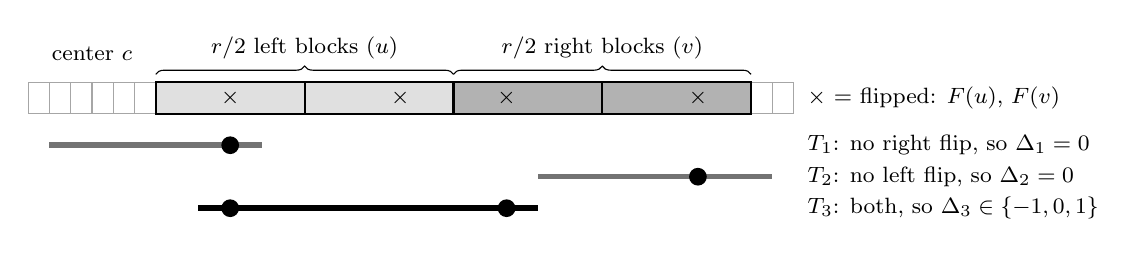
\begin{tikzpicture}[x=0.27cm,y=0.40cm,font=\footnotesize]
 \foreach \x in {0,...,35} \draw[black!35] (\x,0) rectangle ++(1,1);
 \fill[black!12] (6,0) rectangle (13,1);  \fill[black!12] (13,0) rectangle (20,1);
 \fill[black!30] (20,0) rectangle (27,1); \fill[black!30] (27,0) rectangle (34,1);
 \foreach \a in {6,13,20,27} \draw[thick] (\a,0) rectangle ++(7,1);
 \draw[decorate,decoration={brace,amplitude=3pt}] (6,1.25) -- (20,1.25) node[midway,above=2pt]{$r/2$ left blocks ($u$)};
 \draw[decorate,decoration={brace,amplitude=3pt}] (20,1.25) -- (34,1.25) node[midway,above=2pt]{$r/2$ right blocks ($v$)};
 \node at (3,1.9) {center $c$};
 \node at (9.5,0.5) {$\times$};  \node at (17.5,0.5) {$\times$};
 \node at (22.5,0.5) {$\times$}; \node at (31.5,0.5) {$\times$};
 \node[anchor=west] at (36.2,0.5) {$\times$ = flipped: $F(u)$, $F(v)$};
 \draw[line width=2pt,black!55] (1,-1) -- (11,-1);   \node[anchor=west] at (36.2,-1) {$T_1$: no right flip, so $\Delta_1=0$};
 \draw[line width=2pt,black!55] (24,-2) -- (35,-2);  \node[anchor=west] at (36.2,-2) {$T_2$: no left flip, so $\Delta_2=0$};
 \draw[line width=2pt,black]    (8,-3) -- (24,-3);   \node[anchor=west] at (36.2,-3) {$T_3$: both, so $\Delta_3\in\{-1,0,1\}$};
 \foreach \x/\y in {9.5/-1,22.5/-3,9.5/-3,31.5/-2} \fill (\x,\y) circle (3.2pt);
\end{tikzpicture}

\caption{A product-star cell. The cell fixes a center $c$ and, in each of $r$ blocks of
$b=2^s-1$ coordinates, lets the point move within a Hamming-code star (no flip or one flip); the left
pattern $u$ uses $r/2$ blocks and the right pattern $v$ the other $r/2$. A gate contributes to the
mixed residual only if it reads a coordinate flipped by $u$ and one flipped by $v$.}
\label{fig:cell}
\end{figure}


\paragraph{A sampler that never sees one-sided behavior.}
The value of the circuit on the cell is
\(g(s^{\rm L}(u)+s^{\rm R}(v)+R(u,v))\), and we must estimate its
average over the \(N^2\) points. Expand the lookup in characters of a
cyclic group \(\Z/\Omega\), taking \(\Omega=4mG+1\) for \(G\)
bottom gates, where \(m=4\) is the moment order of the trace bound below. This exceeds the score range
and the absolute value of every signed sum of \(2m\) residuals:
\(g(s)=\sum_\theta\widehat g(\theta)\omega^{\theta s}\) with
\(\omega=e^{2\pi\iu/\Omega}\). Then
\[
 \omega^{\theta s(u,v)}
 =\underbrace{\omega^{\theta s^{\rm L}(u)}}_{\text{\fontsize{9}{10.8}\selectfont depends on }u}\;
  \underbrace{\omega^{\theta s^{\rm R}(v)}}_{\text{\fontsize{9}{10.8}\selectfont depends on }v}\;
  \underbrace{\omega^{\theta R(u,v)}}_{=:M_\theta(u,v)} .
\]
The first two factors are arbitrary unimodular \emph{selectors}, one
on each side; this separation is the standard finite Fourier
expansion, as in~\cite[Equation~(29)]{Nag72}.
That preprint introduced a universal sampler:
one list of \(Q\) sample pairs \((U_j,V_j)\) that estimates
\(a^{\mathsf T}Mb/N^2\) for all selectors \(a,b\) at once, provided the
sampling error matrix of \(M\) has small operator norm. We apply the
sampler separately to the real matrices
\(D_{\theta,0}=\operatorname{Re}M_\theta\) and
\(D_{\theta,1}=\operatorname{Im}M_\theta\).
For each real error matrix \(E\), its norm is controlled by
\(\tr\bigl((EE^{\mathsf T})^m\bigr)\). The sample list can be chosen
deterministically, bit by bit, if the algorithm can compute
conditional expectations of this potential exactly~\cite[Appendix~F]{Nag72}.
So the one-sided parts of the circuit, however complicated, never
enter the object that must be computed; only the matrices
\(M_\theta\) do.

\paragraph{The cycle-sum identity.}
Expanding \(\tr\bigl((EE^{\mathsf T})^m\bigr)\) gives a sum over closed walks
\(w\) of length \(2m\) that alternate between left and right
patterns. Expanding the cosine and sine entries of the real
matrices gives characters of \emph{signed sums} of residuals along
the \(2m\) edges, and summing over all frequencies \(\theta\) turns
the character into an indicator:
\(\sum_\theta\omega^{\theta Y}=\Omega\cdot\ind[Y=0]\) when
\(|Y|<\Omega\). The result (\cref{lem:cycle}) is that the potential,
summed over frequencies, is a weighted count of closed walks whose
signed residual sums
\[
 Y_\sigma(w)=\sum_{l=1}^{2m}\sigma_lR(e_l)
\]
vanish, over sign patterns \(\sigma\in\{\pm1\}^{2m}\). The lookup has
disappeared. What remains is one integer per circuit and walk, a sum of
local contributions of the bottom gates. If each edge has population
at most \(U\), the total absolute contribution is at most \(2mU\).

For example, a four-edge walk visits a rectangle of left and right
choices. One sign pattern tests the alternating sum of its four
residual values. Summing the characters turns this into the exact
condition that this signed sum is zero. \Cref{lem:cycle} gives the
full identity, including all sign patterns, masks, and pair calls.
For a pair call there are two walk sums, and the potential is a
weighted sum of joint zero tests \(\ind[Y_1=0]\ind[Y_2=0]\); after
localization, \cref{thm:modular-tomography} reconstructs their joint
distribution.

\paragraph{Localize and reconstruct ($5/2$).}
Counting walks with \(Y_\sigma(w)=0\) is the problem that the
author's near-cubic gate preprint~\cite[Sections~4--6]{NagCG} solves
for the scores of restricted circuits. Subsampling the bottom gates at
nested rates writes the integer \(Y\) through a few short integer
\emph{digits}; once the digits are fixed, \(Y\) is confined to an
interval about \(P\) times shorter than its population. Here \(P\)
is a prime scale of order \(n/\polylog n\): the algorithm evaluates
polynomials of degree about \(P\) over all \(2^{n-k}\) cells at once
by Williams' rectangular matrix multiplication, so it can count
residues modulo every prime in \((P/2,P]\); the Beigel--Tarui lifting polynomial~\cite{BT94} lifts the corresponding residue indicators to powers of \(p\), letting the printer recover the counts exactly. Pair calls have two circuits and hence two scores; their localized
joint distribution must be reconstructed. The printing procedure of
\cref{sec:printing} computes the modular count tables in batches, reducing each table to rectangular matrix multiplication.

Under the quantitative size condition of \cref{earlier:g:lem:two-window},
prime residue counts determine all short line projections, and hence
the joint distribution on a box of side about \(P^{3/2}\).
To our knowledge, this is the first use of discrete tomography in circuit complexity; the method was introduced for this purpose in~\cite{NagCG}.
Within the algorithmic method, modular counting (e.g.~\cite{Wil13,ACW16}) computes residues of a single count; here many residue counts jointly determine a whole two-score distribution.
Reconstructing a \(0/1\) lattice set from its line sums is NP-hard already for three directions~\cite{GGP99}.
Here the unknown is an integer-valued function on a box of side about \(P^{3/2}\), and Hajdu and Tijdeman's algebraic theory~\cite{HT01} shows that enough directions determine it uniquely. Recovery is therefore an exact linear system, with at most \(P^4\) unknowns and \(0/1\) coefficients, solved in polynomial time by fraction-free elimination~\cite{Bareiss68}.
Thus walk sums with population up to \(U\approx P^{5/2}\) can be handled exactly.

\par\noindent\begin{minipage}{\linewidth}
\begin{theorem}[Modular discrete tomography]\label{thm:modular-tomography}
Let \(\mathcal P\) be a finite nonempty set of primes, \(D'=1+\sum_{p\in\mathcal P}(p-1)\), and \(S(q)=\sum_{m=1}^{q}m\varphi(m)\), where \(\varphi\) is Euler's totient.
For \(a,b\in\Z\) and \(L\in\N\) with \(2\le L\le S(\lfloor(D'-1)/(L-1)\rfloor)\), every \(f:B\to\Q\) on the known box \(B=([a,a+L)\times[b,b+L))\cap\Z^2\) is determined by its exact rational sums
\(F_p(r,s)=\sum_{(x,y)\in B,\;(x,y)\equiv(r,s)\bmod p}f(x,y)\), for \(p\in\mathcal P\), \(r,s\in\Z/p\Z\).
Exact elimination recovers \(f\) in time polynomial in \(L\), \(\sum_{p\in\mathcal P}p^2\), and the total binary input length, including the box endpoints and rational sums.
\end{theorem}
\end{minipage}\par\smallskip
The uniqueness and exact-inverse assertions are formalized as
\path{NearCubicGates.Reconstruction.pairMatrix_injective} and
\path{pair_reconstruction_complete} in the Lean companion.
\begin{proof}
\Cref{earlier:g:lem:two-window} proves uniqueness; fraction-free elimination~\cite{Bareiss68} on the \(0/1\) residue matrix gives recovery with polynomial bit cost, as in \cref{prop:time}.
\end{proof}

\begin{corollary}[Prime-window tomography]\label{cor:prime-window-tomography}
There are absolute constants \(c>0\) and \(P_0\) such that, for every integer \(P\ge P_0\), taking \(\mathcal P\) to be all primes in \((P/2,P]\), \cref{thm:modular-tomography} applies to every known integer box of side \(2\le L\le cP^{3/2}/(\log P)^{3/4}\).
\end{corollary}
\begin{proof}
\Cref{earlier:g:lem:window-size,earlier:g:lem:primes} give an admissible side of order \(D'^{3/4}=\Theta(P^{3/2}/(\log P)^{3/4})\). The size condition is preserved when \(L\ge2\) decreases.
\end{proof}
For one score, exact residue sums for the same prime set determine a rational function on a known interval of at most \(D'\) consecutive integers (\cref{earlier:g:lem:one-window}; Lean: \path{NearCubicGates.ScalarWindow.frameResidueData_injective}).

\paragraph{The exponent.}
Combining the two estimates,
\[
 \frac{W}{n^{3/2}}\lesssim U\lesssim P^{5/2}
 \qquad\Longrightarrow\qquad
 W\lesssim
 \underbrace{n^{3/2}}_{\text{\fontsize{9}{10.8}\selectfont star cells}}\;
 \underbrace{P}_{\text{\fontsize{9}{10.8}\selectfont localization}}\;
 \underbrace{P^{3/2}}_{\text{\fontsize{9}{10.8}\selectfont reconstruction}}
 \approx n^4 .
\]
The gain is charged per wire, so sparse gates are handled according
to the inputs they read.



\paragraph{One mask for every prime.}
Points of abnormally large population must be discarded by a
\emph{mask}, and the mask enters the polynomials whose residues are
counted modulo many odd primes. The masks of~\cite{Nag72}
are polynomials over \(\F_2\) whose integer lifts are exact only modulo
powers of two, so they cannot be used there. Our mask (\cref{sec:masks}) is an exact
integer polynomial: if \(X\) counts the subsampled bottom gates with
nonzero residual at a point, then
\[
 \ind[X\le\tau]=\sum_{a=0}^{\Xmax}c_a\binom Xa
 \qquad(0\le X\le\Xmax)
\]
with integers \(c_a\) given by Newton forward differences, and
\(\binom Xa\) is the elementary symmetric polynomial of degree \(a\)
in the Boolean residual indicators. A single moment test certifies
\(X\le\Xmax\) on a whole cell. The identity holds over \(\Z\), so the
mask is correct modulo every integer at once.

\paragraph{Main components.}
Lean names below have prefix \path{NearQuarticWires.}; the full hypotheses are in the indicated statements.
\begin{center}\footnotesize
\begin{tabularx}{\textwidth}{@{}>{\raggedright\arraybackslash}p{.16\textwidth}X>{\raggedright\arraybackslash}p{.09\textwidth}>{\raggedright\arraybackslash}p{.31\textwidth}@{}}
\toprule
Tool & Statement & Where & Lean name\\\midrule
Modular tomography & Joint residue tables determine a rational box function under an explicit window criterion. & Thm.~\ref{thm:modular-tomography} & {\footnotesize\texttt{\mbox{Tomography.}\allowbreak\mbox{residueCounts\_determine}}}\\[2pt]
Integer threshold masks & Exact bounded-population cutoff, with integer coefficients, valid modulo every integer. & Lem.~\ref{lem:maskpoly} & {\footnotesize\texttt{\mbox{Mask.}\allowbreak\mbox{cutoff\_eq\_newton\_sum\_of\_le}}}\\[2pt]
Cycle-sum identity & A Fourier trace sum counts zero signed walk sums; Lean checks \(m=4\). & Lem.~\ref{lem:cycle} & {\footnotesize\texttt{\mbox{Cycle.}\allowbreak\mbox{cycle\_sum\_identity}}}\\[2pt]
Product-star population & Some partition has mean mixed population at most \(6r^{3/2}W/n^{3/2}\). & Lem.~\ref{lem:meanpop} & {\footnotesize\texttt{\mbox{Cells.}\allowbreak\mbox{mean\_population}}}\\[2pt]
Certified counting & Every witness is sound; a short witness is precise below \(a\beta\mathcal A_4(n)\). & Thm.~\ref{thm:counter} & {\footnotesize\texttt{\mbox{Program.}\allowbreak\mbox{counterExists4}}}\\[2pt]
Wire transfer & The full quartic counter contract yields a.e. constant-error \(\ENP\) hardness. & Thm.~\ref{thm:wire-transfer} & {\footnotesize\texttt{\mbox{Transfer.}\allowbreak\mbox{transfer4\_official}}}\\
\bottomrule
\end{tabularx}
\end{center}

\paragraph{Where the method stops.}
\begin{itemize}[leftmargin=*,nosep]

\item Two-score reconstruction handles walk sums of population up to about \(P^{5/2}\) (the window condition \eqref{eq:window}), and the degree of the printed polynomials keeps \(P\) below about \(n\) (by \eqref{eq:prime-budget}). The \(P^{3/2}\) window is sharp up to logarithmic factors for recovering arbitrary box distributions from residue data (\cref{earlier:g:rem:rank}).
\item Arbitrary real top weights lack this bounded integer-score guarantee; the fixed-error transfer gives no vanishing correlation. Extensions remain open; these are limits of this method (\cref{sec:scope}).
\end{itemize}

\paragraph{Published foundations.}\label{par:five-inputs}
The formal proof assumes exactly \publishedinputcount\ published results from
 four\ papers, listed with exact locators in \cref{sec:formal}.
The BCGT13 verifier input is Theorem~11.1, at the parameter tuple \((2,4,0,1)\) used in this paper~\cite{BCGT13}.
Everything else the formal proof uses is proved in Lean, including the short PCP of Murray--Williams~\cite{MW20}, the refuter and amplification interfaces of Chen--Lyu--Williams~\cite{CLW20}, integer normalization of threshold gates, concentration, and the prime counts from Chebyshev-type bounds.
\Cref{app:earlier} restates and proves the PCP, refuter and amplification components, with their origins credited; the classical normalization, concentration and prime-count facts are cited to their published sources in \cref{app:statements} and \cref{earlier:g:lem:primes}.

\subsection{The formal statement}\label{sec:formal}
The formalization is available at \leanrepo\ (release tag \texttt{v1.0}).
The following verbatim definitions in \texttt{Proof/Quartic/Statement/Joint.lean}
state \cref{thm:main,thm:gates} with shared constants and the rejection gap \(\gamma\) quantified existentially (some rational \(0<\gamma<1\)); \texttt{wireCap} and \texttt{gateCap} are the two boxed caps, and \texttt{InENP} defines \(\ENP\) by an explicit oracle machine:
\begingroup
\lstset{basicstyle=\small\ttfamily,columns=fullflexible,keepspaces=true,
 breaklines=true,breakatwhitespace=true,breakindent=6em,showstringspaces=false,
 frame=single,aboveskip=4pt,belowskip=4pt,
 literate={∀}{{$\forall$}}1 {∃}{{$\exists$}}1 {ℝ}{{$\mathbb R$}}1
 {ℚ}{{$\mathbb Q$}}1 {ℕ}{{$\mathbb N$}}1 {→}{{$\to$}}1
 {∧}{{$\land$}}1 {≤}{{$\le$}}1 {₀}{{\textsubscript{0}}}1}
\lstinputlisting{joint-statement-verbatim.txt}
\endgroup
The release type is \texttt{ReleaseStatement := PublishedInputs}
\(\to\) \texttt{JointStatement4}. Its
\publishedinputcount\ inputs are transcribed in their source models:
\begin{center}\footnotesize
\begin{tabularx}{\textwidth}{@{}lX@{}}\toprule
Source & Exact published locator\\\midrule
Williams~\cite{WilACC14} & Cor.~4.4, p.~2:17 (also Cor.~C.2, p.~2:29).\\
BCGT~\cite{BCGT13} & Theorem~11.1, at the parameter tuple \((2,4,0,1)\) used in this paper; p.~51 (ECCC rev.~3).\\
BCGT~\cite{BCGT13} & Alg.~17, p.~124 (ECCC rev.~3).\\
Sudan--Trevisan--Vadhan~\cite{STV01} & Thm.~29, p.~17 (ECCC rev.~2).\\
Chen--Williams~\cite{CW19} & Lem.~22, p.~19:15, soundness \(1/2\).\\
Chen--Williams~\cite{CW19} & Lem.~26, p.~19:16.\\

\bottomrule\end{tabularx}
\end{center}
Running \texttt{lake env lean Check.lean} prints the axiom list:
\begin{center}\small\texttt{[propext, Classical.choice, Quot.sound]}\end{center}
The companion's source mapping quotes each published statement beside
its transcription and records the modeling conventions; this
faithfulness comparison is separate from kernel checking.
The trusted files are \texttt{Statement.lean} and \texttt{Final.lean},
\texttt{Joint.lean}, and \texttt{Release.lean} in
\texttt{Proof/Quartic/Statement/}. They define the machine and circuit
models, measures, published premises and conclusion; everything else
is checked by the kernel. A full build is a large computation; the
companion's README lists its requirements.

Generative AI tools were used substantively throughout this work, including proof search, parameter selection, drafting, and the construction of the Lean formalization; see the AI methodology statement at the end of the paper. The correctness of both theorems, as formally stated, rests on the kernel-checked proof described above.

\subsection{Organization}\label{sec:roadmap}

\Cref{fig:proof-dag} gives the architecture.
\begin{description}[nosep,leftmargin=3.1em,labelwidth=2.6em,font=\normalfont]
\item[\S2] The counting theorem (matrix concentration is in Appendix~\ref{app:statements}).
\item[\S3] Product-star cells and their mixed residuals.
\item[\S4] Sampling bounded real matrices.
\item[\S5] The cycle-sum identity and its computation.
\item[\S6] Exact integer polynomial masks.
\item[\S7] Localization and certification of walk sums.
\item[\S8] Exact printing of the modular tables.
\item[\S9] The counting algorithm.
\item[\S10] Soundness, completeness and running time.
\item[\S11] The parameter choices and quartic wire cap.
\item[\S12] The almost-everywhere lower-bound transfer.
\item[\S13] Scope.
\end{description}
The appendices give the wire-measure transfer, notation, attribution,
and the statements and proofs from earlier work.

\section{The counting theorem}\label{sec:prelim}

This section states the counting guarantee. Supporting statements
and their complete proofs are in \cref{app:statements,app:earlier}.
The published foundations are identified
in \cref{par:five-inputs}.

\subsection{Normalized calls and the counting theorem}\label{sec:counting}

A \emph{call} asks for the acceptance
probability of one of three predicates on \(\{0,1\}^n\): one circuit
\(C^1\); the exclusive-or \(C^1\oplus C^2\) of two circuits; or
\(C^1\oplus\PAR_\Sigma\), where \(\PAR_\Sigma(x)=\bigoplus_{i\in\Sigma}x_i\)
is an explicit input parity. We call these \emph{single},
\emph{pair} and \emph{parity} calls and write \(\pred\) for the
predicate. Let \(n\ge4\) and
\[
 B_0=4n\lceil\lgx(n+1)\rceil .
\]
A call is \emph{normalized} if its circuits are \(\SYM\circ\THR\)
circuits on \(n\) inputs whose bottom weights and thresholds are
integers of magnitude below \(2^{B_0}\), with explicit lookup tables,
and whose total wire count satisfies \(W=W(C^1)+W(C^2)\le2n^4\)
(with \(W(C^2)=0\) for single and parity calls). The call also
contains a rational radius \(\beta\) with
\(n^{-B_1}\le\beta\le1/16\), encoded in at most \(n^{B_2}\) bits, for
fixed positive integers \(B_1,B_2\).

Every single, pair or parity call made from \(\SYM\circ\THR\) circuits with total wire count at most \(2n^4\) can be put into the integer-parameter form above, with the same bottom gates and no more wires. Indeed, apply \cref{imp:integer} to each
bottom gate as a function of the \(f\ge1\) inputs it reads (a gate of
fan-in zero is a constant and is written \(\ind[0\ge\theta]\) with
\(\theta\in\{0,1\}\)): its new weights and threshold are integers in
\(\pm f^f\), and \(f^f\le n^n<2^{B_0}\). No new input is read, so the
wire count does not increase. Running times are counted in steps of a deterministic multitape Turing machine.

\begin{theorem}[Certified counting below the quartic wire cap]
\label{thm:counter}
Fix positive integers \(B_1,B_2\). There are a constant
\(a=a_{B_1,B_2}>0\) and one deterministic algorithm whose input is a
call on \(n\) inputs and a binary string, the
\emph{witness}, with the following properties.
\begin{enumerate}[(i)]
\item (Soundness) For every witness, it returns dyadic rationals
\((\phat,\khat)\) with \(|\phat-\Pr_x[\pred(x)=1]|\le\khat\).
\item (Completeness) For all sufficiently large \(n\), on every normalized call, if
\(W\le a\,\beta\,\mathcal A_4(n)\), some witness of polynomial length
gives \(\khat\le\beta\).
\item (Time) For all sufficiently large \(n\), on every normalized
call and every witness it halts within \(2^n/n^{\mu_n}\) steps, reads
a prefix of polynomial length of the witness, and uses no oracle.
Hence any prescribed fixed polynomial number of calls has total
workload \(2^nn^{O(1)-\mu_n}\).
\item (Interface) Its outputs are dyadic with denominators dividing
\(2^{n+1}\) and encoded length polynomial in \(n\). On an input that is
not a normalized call it returns \((1/2,1/2)\) in time polynomial in
the encoded length of the call, independently of the witness.
\end{enumerate}
\end{theorem}
Lean: \path{NearQuarticWires.Program.counterExists4}, from Williams' rectangular-product input.


The same cap handles all three call types; this is sufficient for
the transfer. \Crefrange{sec:cells}{sec:asymptotics} prove
\cref{thm:counter}.

The standard matrix concentration inequality used below is
\cref{imp:tropp} in \cref{app:statements}; throughout,
\(\|\cdot\|\) is the operator norm.

\section{The call on product-star cells}\label{sec:cells}

This section rewrites a call on one cell. Each score splits into a
part that depends only on the left pattern, a part that depends only
on the right pattern, and a mixed residual (\cref{lem:identity}). The
mixed residual is rare (\cref{lem:mixed,lem:meanpop}), and a Fourier
expansion moves everything except the residual into one-sided
selectors (\cref{lem:fourier}).

Fix a normalized call and one of the \(2^k\) partitions of
\cref{imp:partition}; its index is part of the witness. Recall from
there that a cell has an address \(z\in\{0,1\}^{n-k}\), its
\emph{column}, a center \(c(z)\), and points \(c(z)\oplus u\oplus v\);
the left pattern \(u\in[N]\) flips at most one coordinate in each of
\(r/2\) blocks of \(b=2^s-1\) coordinates, the right pattern \(v\)
likewise in the other \(r/2\) blocks, and \(F(u)\) is the set of
coordinates flipped by \(u\). Let
\(\cJ\subseteq\{1,2\}\) be the set of circuits of the call
(\(\cJ=\{1,2\}\) for pair calls and \(\cJ=\{1\}\) otherwise). Circuit
\(j\in\cJ\) has bottom gates \(T_{j,1},\dots,T_{j,G_j}\) and lookup
\(g_j\); put \(G_2=0\) if \(2\notin\cJ\). For a column \(z\), write
\(c=c(z)\) and define, for \(u,v\in[N]\),
\begin{align*}
 \Delta_{j,i}(z,u,v)&=T_{j,i}(c\oplus u\oplus v)-T_{j,i}(c\oplus u)-T_{j,i}(c\oplus v)+T_{j,i}(c),
 \qquad R_j=\sum_{i}\Delta_{j,i},\\
 s^{\rm L}_j(z,u)&=\sum_i\bigl(T_{j,i}(c\oplus u)-T_{j,i}(c)\bigr),
 \qquad s^{\rm R}_j(z,v)=\sum_iT_{j,i}(c\oplus v),\\
 s_j(z,u,v)&=\sum_iT_{j,i}(c\oplus u\oplus v),
 \qquad \pop(z,u,v)=\sum_{j\in\cJ}\sum_i|\Delta_{j,i}(z,u,v)|.
\end{align*}
We call \(s_j\) the \emph{score} of circuit \(j\), \(\Delta_{j,i}\) the
\emph{mixed residual} of the bottom gate \((j,i)\), and \(\pop\) the
\emph{population} of the point. The values \(T_{j,i}(c\oplus x)\) for
\(x\in\{0,u,v,u\oplus v\}\) are the \emph{atoms} of the bottom gate at
the point.

Throughout, \(\Delta_{j,i}\) is used only as the integer linear form
displayed above in four atoms, and \(|\Delta_{j,i}|=\Delta_{j,i}^2\)
(by \cref{imp:range}) only as an integer quadratic form. No
representation of a residual over \(\F_2\) is used.

\begin{lemma}[Exact score identity]\label{lem:identity}
\(s_j=s^{\rm L}_j+s^{\rm R}_j+R_j\) at every point,
\(s_j\in[0,G_j]\), and \(|R_j|\le G_j\).
\end{lemma}
\begin{proof}
Summing the definitions gives
\(s^{\rm L}_j+s^{\rm R}_j+R_j=\sum_iT_{j,i}(c\oplus u\oplus v)\). The
range claims follow from \(T\in\{0,1\}\) and \(\Delta\in\{-1,0,1\}\).
\end{proof}

\begin{lemma}[Mixed dependence]\label{lem:mixed}
If \(\Delta_{j,i}(z,u,v)\ne0\), then \(T_{j,i}\) has a nonzero weight on
some coordinate of \(F(u)\) and on some coordinate of \(F(v)\).
Consequently, if \(d_l\) is the number of bottom gates, of all circuits
of the call, with nonzero weight on coordinate \(l\), then for every
column \(z\)
\[
 \pop(z,u,v)\le\min\Bigl\{\sum_{l\in F(u)}d_l,\ \sum_{l\in F(v)}d_l\Bigr\}.
\]
\end{lemma}
\begin{proof}
If \(T=T_{j,i}\) has zero weight on all of \(F(u)\), then
\(T(c\oplus u\oplus v)=T(c\oplus v)\) and \(T(c\oplus u)=T(c)\), so
\(\Delta=0\); symmetrically for \(F(v)\). Each bottom gate with nonzero
residual is therefore incident to \(F(u)\), and also to \(F(v)\).
\end{proof}

\begin{lemma}[Product-star mean population]\label{lem:meanpop}
Let \(r\) be even with \(2\le r\le n/4\), set \(s=\lfloor\log_2(n/r+1)\rfloor\), \(b=2^s-1\), and \(k=rs\).
Use \(r\) disjoint blocks of \(b\) coordinates, split equally between left and right, and a binary Hamming code whose parity-check columns are the nonzero vectors of \(\F_2^s\).
Choosing a code coset in each block gives \(2^k\) partitions into products of stars, each with \(2^{n-k}\) cells and \(2^k\) points per cell; other coordinates belong to the center.
Let \(T_1,\ldots,T_G\) be integer-parameter Boolean threshold gates with fan-ins \(f_i\), counted with repetition, and \(\sum_i f_i\le W\). Define
\[
 \Delta_i(c,u,v)=T_i(c\oplus u\oplus v)-T_i(c\oplus u)-T_i(c\oplus v)+T_i(c),
 \qquad \pop(z,u,v)=\sum_i|\Delta_i(c(z),u,v)|.
\]
For a uniform partition index \(\sigma\), uniform cell \(z\), and independent uniform left and right star patterns \(u,v\),
\[
 \E_{\sigma,z,u,v}\pop(z,u,v)\le6r^{3/2}W/n^{3/2}.
\]
Consequently some fixed partition has the same bound on \(\E_{z,u,v}\pop(z,u,v)\).
\end{lemma}
Lean: \path{NearQuarticWires.Cells.average_population_le} and \path{Cells.mean_population}. This is the product-star estimate from~\cite[Appendix~A]{Nag72}, used here by the collective cycle analysis.

\begin{proof}
Averaged over the partition index and the column, which together give
a uniform center independent of the patterns (\cref{imp:partition}),
\cref{imp:population} gives
\(\Pr[\Delta_i\ne0]\le2f_i/(b+1)^{3/2}\le2f_i(2r/n)^{3/2}\le6r^{3/2}f_i/n^{3/2}\),
using \(b+1>n/(2r)\). Sum over bottom gates and choose a partition index
whose mean is at most the average.
\end{proof}

\subsection{Fourier decomposition with the mask inside the matrix}\label{sec:fourier}

Fix the trace order \(m=4\). Put \(\Omega_j=4mG_j+1\) for
\(j\in\cJ\) and \(\Omega_2=1\) if \(2\notin\cJ\), let
\(\Theta=\Z/\Omega_1\times\Z/\Omega_2\),
\(\omega_j=e^{2\pi\iu/\Omega_j}\), and let \(M_F=\lceil\sqrt{|\Theta|}\,\rceil\), the least integer with \(M_F^2\ge|\Theta|\). The
modulus \(\Omega_j>2mG_j\) exceeds every score, which lies in
\([0,G_j]\), and the absolute value of every walk sum used later,
which is at most \(2mG_j\) (\cref{lem:cycle}).

\begin{lemma}[Fourier decomposition]\label{lem:fourier}
For each call there are complex numbers \(\widehat F(\theta,\nu)\),
\((\theta,\nu)\in\Theta\times\{0,1\}\), with
\(\sum_{\theta,\nu}|\widehat F(\theta,\nu)|\le M_F\), and for every
column \(z\) functions
\(a_{z,\theta,\nu},b_{z,\theta,\nu}:[N]\to\C\) of modulus at
most one, such that for every \((u,v)\) and every
\(\mu_0\in\{0,1\}\)
\[
 \pred\bigl(c(z)\oplus u\oplus v\bigr)\,\mu_0
 =\sum_{\theta,\nu}\widehat F(\theta,\nu)\,a_{z,\theta,\nu}(u)\,b_{z,\theta,\nu}(v)\,
 \omega_1^{\theta_1R_1(z,u,v)}\omega_2^{\theta_2R_2(z,u,v)}\,\mu_0 .
\]
\end{lemma}
\begin{proof}
\emph{Single and pair calls.} Define \(F\) on \(\Theta\) by
\(F(t_1,t_2)=g_1(t_1)\) (single) or \(g_1(t_1)\oplus g_2(t_2)\) (pair)
for \((t_1,t_2)\in[0,G_1]\times[0,G_2]\), and \(F=0\) elsewhere; this
is well defined because \(\Omega_j>G_j\). Put
\(\widehat F(\theta,0)=|\Theta|^{-1}\sum_tF(t)\omega_1^{-\theta_1t_1}\omega_2^{-\theta_2t_2}\)
and \(\widehat F(\theta,1)=0\). Character orthogonality on the finite
group \(\Theta\) gives
\(F(t)=\sum_\theta\widehat F(\theta,0)\omega_1^{\theta_1t_1}\omega_2^{\theta_2t_2}\),
Parseval gives
\(\sum_\theta|\widehat F(\theta,0)|^2=|\Theta|^{-1}\sum_tF(t)^2\le1\),
and the Cauchy--Schwarz inequality gives \(\sum_\theta|\widehat F|\le\sqrt{|\Theta|}\le M_F\).
By \cref{lem:identity}, \(\pred=F(s_1,s_2)\) and
\(\omega_j^{\theta_js_j}=\omega_j^{\theta_js^{\rm L}_j}\omega_j^{\theta_js^{\rm R}_j}\omega_j^{\theta_jR_j}\).
Take \(a_{z,\theta,0}(u)=\prod_j\omega_j^{\theta_js^{\rm L}_j(z,u)}\)
and \(b_{z,\theta,0}(v)=\prod_j\omega_j^{\theta_js^{\rm R}_j(z,v)}\).

\emph{Parity calls.} By linearity,
\(\PAR_\Sigma(c\oplus u\oplus v)=\PAR_\Sigma(c)\oplus\PAR_\Sigma(u)\oplus\PAR_\Sigma(v)\).
Let \(\chi_0=(-1)^{\PAR_\Sigma(c(z))}\), \(\chi_{\rm L}(u)=(-1)^{\PAR_\Sigma(u)}\),
\(\chi_{\rm R}(v)=(-1)^{\PAR_\Sigma(v)}\), and let
\(\Gamma_g(t)=(-1)^{g_1(t)}\) on \([0,G_1]\) and \(\Gamma_g=0\)
elsewhere on \(\Z/\Omega_1\). Then
\[
 \pred=\tfrac12-\tfrac12\,\chi_0\chi_{\rm L}(u)\chi_{\rm R}(v)\,\Gamma_g(s_1).
\]
Let \(\widehat F(0,0)=\tfrac12\) with \(a_{z,0,0}=b_{z,0,0}=1\),
\(\widehat F(\theta,0)=0\) for \(\theta\ne0\), and
\(\widehat F(\theta,1)=-\tfrac12\widehat\Gamma_g(\theta)\) with
\(a_{z,\theta,1}=\chi_0\chi_{\rm L}\,\omega_1^{\theta_1s^{\rm L}_1}\) and
\(b_{z,\theta,1}=\chi_{\rm R}\,\omega_1^{\theta_1s^{\rm R}_1}\). As above
\(\sum_\theta|\widehat\Gamma_g(\theta)|\le\sqrt{\Omega_1}\), so the total
mass is at most \(\tfrac12+\tfrac12\sqrt{\Omega_1}\le\sqrt{\Omega_1}\le M_F\).
\end{proof}

For a \(0/1\) matrix \(\mask(z)\) on \([N]^2\), defined in
\cref{sec:masks}, put
\[
 M_\theta(z)[u,v]=\omega_1^{\theta_1R_1(z,u,v)}\omega_2^{\theta_2R_2(z,u,v)}\mask(z,u,v),\qquad
 D_{\theta,0}(z)=\operatorname{Re}M_\theta(z),\quad D_{\theta,1}(z)=\operatorname{Im}M_\theta(z).
\]
These \(I=2|\Theta|\) real matrices have entries in \([-1,1]\). They
depend on the circuits, the partition and the mask, but not on the
lookups or the parity set: the lookups and the parity enter only
through the coefficients \(\widehat F\) and the selectors.
The second index of \(D\) specifies the real or imaginary part,
independently of the selector index in \cref{lem:fourier}.

\section{Sampling bounded real matrices}\label{sec:sampler}

A list of \(Q\) sample pairs estimates the average of a matrix
\(D\) against selectors \(a,b\) with an error governed by the operator
norm of one error matrix, uniformly in the selectors. This section
shows that the fixed-moment analysis of~\cite[Lemma~F.1]{Nag72},
written there for \(0/1\) matrices, holds for real matrices with
entries in \([-1,1]\), and records the two consequences we use. In
this section \(m\) is any positive integer; the algorithm uses
\(m=4\).

For a list of \(Q\) pairs \((U_j,V_j)\in[N]^2\) let
\[
 \Gamma(x)=Q-N^2\,\#\{j:(U_j,V_j)=x\}\qquad(x\in[N]^2).
\]
For a real \(N\times N\) matrix \(D\), the error matrix
\(E_D=QD-N^2\sum_jD(U_j,V_j)e_{U_j}e_{V_j}^{\mathsf T}\) satisfies
\begin{equation}\label{eq:ED}
 E_D[x]=D[x]\,\Gamma(x)\qquad(x\in[N]^2),
\end{equation}
since the \(x\) entry of the sum counts the samples at \(x\). Let
\(\cH(E)=\bigl(\begin{smallmatrix}0&E\\E^{\mathsf T}&0\end{smallmatrix}\bigr)\);
for real \(E\) with singular values \(s_i\),
\(\tr\cH(E)^{2m}=2\sum_is_i^{2m}\).

\begin{lemma}[Trace bound for entries in {$[-1,1]$}]\label{lem:tracebound}
If \(D\) is real with entries in \([-1,1]\) and the pairs are
independent and uniform, then
\(\E\tr\cH(E_D)^{2m}\le4N^2((4QN^3)^mm!+(8N^2/3)^{2m}(2m)!)\).
\end{lemma}
\begin{proof}
\(E_D=\sum_{j=1}^QX_j\) with independent
\(X_j=D-N^2D(U_j,V_j)e_{U_j}e_{V_j}^{\mathsf T}\). We check the
hypotheses of \cref{imp:tropp}.
(1) \(\E[N^2D(U,V)e_Ue_V^{\mathsf T}]=\sum_{u,v}D(u,v)e_ue_v^{\mathsf T}=D\),
so \(\E X_j=0\).
(2) \(\|D\|\le\|D\|_F\le N\), so \(\|X_j\|\le N+N^2\le2N^2\).
(3) \(\E X_jX_j^{\mathsf T}=N^2\diag_u(\sum_vD(u,v)^2)-DD^{\mathsf T}\preceq N^3\Id\),
because \(\sum_vD(u,v)^2\le N\) and \(DD^{\mathsf T}\succeq0\); likewise
\(\E X_j^{\mathsf T}X_j\preceq N^3\Id\).
With \(L=2N^2\) and \(\sigma^2\le QN^3\), \cref{imp:tropp} gives
\[
 \Pr[\|E_D\|\ge x]\le2N\exp\Bigl(-\frac{x^2}{2(QN^3+2N^2x/3)}\Bigr)
 \le2N\bigl(e^{-x^2/(4QN^3)}+e^{-3x/(8N^2)}\bigr),
\]
since \(2(a+b)\le4\max\{a,b\}\). As
\(\tr\cH(E)^{2m}\le2N\|E\|^{2m}\),
\begin{align*}
 \E\tr\cH(E_D)^{2m}&\le2N\int_0^\infty2mx^{2m-1}\Pr[\|E_D\|>x]\,dx\\
 &\le4N^2\cdot2m\Bigl(\int_0^\infty x^{2m-1}e^{-x^2/(4QN^3)}dx\\
 &\hphantom{{}\le4N^2\cdot2m\Bigl(}+\int_0^\infty x^{2m-1}e^{-3x/(8N^2)}dx\Bigr)\\
 &=4N^2\cdot2m\Bigl(\tfrac12(4QN^3)^m(m-1)!+(8N^2/3)^{2m}(2m-1)!\Bigr)\\
 &=4N^2\bigl((4QN^3)^mm!+(8N^2/3)^{2m}(2m)!\bigr).
\end{align*}
Only (1)--(3) were used about the summands.
\end{proof}
The Lean companion proves the \(m=4\) bound it uses by a direct moment computation, without Tropp's inequality (\path{NearQuarticWires.Sampler.mean_traceMoment_le}).

\begin{lemma}[Uniform error over selectors]\label{lem:selector}
For every column \(z\), sample list and mask, put
\(\varepsilon_z=\max_{\theta,\nu}\|E_{D_{\theta,\nu}(z)}\|/(QN)\). Then
\begin{align*}
 \Bigl|\frac1{N^2}\sum_{u,v}(\pred\cdot\mask)(u,v)-\frac1Q\sum_{j}(\pred\cdot\mask)(U_j,V_j)\Bigr|
 &\le2M_F\,\varepsilon_z,\\
 \Bigl|\frac1{N^2}\sum_{u,v}\mask(u,v)-\frac1Q\sum_{j}\mask(U_j,V_j)\Bigr|&\le\varepsilon_z ,
\end{align*}
where \((\pred\cdot\mask)(u,v)=\pred(c(z)\oplus u\oplus v)\mask(z,u,v)\).
\end{lemma}
\begin{proof}
For \(a,b\in\C^N\) with coordinates of modulus at most one and a real
matrix \(E\), \(|a^{\mathsf T}Eb|\le\|E\|\,\|a\|_2\|b\|_2\le N\|E\|\);
the operator norm of a real matrix is the same over \(\R\) and over
\(\C\). For each \((\theta,\nu)\), take \(a=a_{z,\theta,\nu}\) and
\(b=b_{z,\theta,\nu}\),
\[
 \frac{a^{\mathsf T}M_\theta b}{N^2}-\frac1Q\sum_ja_{U_j}b_{V_j}M_\theta(U_j,V_j)
 =\frac{a^{\mathsf T}(E_{D_{\theta,0}}+\iu E_{D_{\theta,1}})b}{QN^2},
\]
of modulus at most \(2N\cdot QN\varepsilon_z/(QN^2)=2\varepsilon_z\).
Multiply by \(\widehat F(\theta,\nu)\), sum, and apply
\cref{lem:fourier} with \(\mu_0=\mask(z,u,v)\) at each point. For the
second line use \(\theta=0\), \(M_0=\mask=D_{0,0}\) and
\(a=b=\mathbf 1\).
\end{proof}

\begin{lemma}[From a potential bound to an average error]\label{lem:root}
Let \(Z\) be a nonempty finite set of columns, let \(m\ge1\), let
\(0<\eta\le1\), and let \(Q\ge1024Nm\eta^{-2}(4N^2I)^{1/m}\). If real
matrices \(E_t(z)\), \(z\in Z\), \(t\le I\), satisfy
\[
 \sum_{z\in Z}\sum_{t\le I}\tr\cH(E_t(z))^{2m}
 \le|Z|\,I\,4N^2\bigl((4QN^3)^mm!+(8N^2/3)^{2m}(2m)!\bigr),
\]
then \(|Z|^{-1}\sum_{z\in Z}\max_t\|E_t(z)\|/(QN)\le\eta\).
\end{lemma}
\begin{proof}
Since \(\tr\cH(E)^{2m}=2\sum_is_i^{2m}\ge2\|E\|^{2m}\),
\(\max_t\|E_t(z)\|^{2m}\le\frac12\sum_t\tr\cH(E_t(z))^{2m}\). By Jensen's
inequality for \(x\mapsto x^{1/(2m)}\),
\begin{align*}
 \frac1{|Z|}\sum_z\max_t\|E_t(z)\|
 &\le\Bigl(2N^2I\bigl((4QN^3)^mm!+(8N^2/3)^{2m}(2m)!\bigr)\Bigr)^{1/(2m)}\\
 &\le(4N^2I)^{1/(2m)}\Bigl(\sqrt{4QN^3m}+\tfrac{16N^2m}{3}\Bigr),
\end{align*}
using \((x+y)^{1/(2m)}\le x^{1/(2m)}+y^{1/(2m)}\), \(m!\le m^m\) and
\((2m)!\le(2m)^{2m}\). Dividing by \(QN\), the bound is
\((4N^2I)^{1/(2m)}(2\sqrt{Nm/Q}+16Nm/(3Q))\). Under the hypothesis on
\(Q\) the first term is at most \(\eta/16\) and the second at most
\(\eta/192\).
\end{proof}

This is the argument of~\cite[Lemma~F.1]{Nag72}, with an arbitrary
set \(Z\) of columns in place of all columns.

\section{The cycle-sum identity}\label{sec:cycle}

The sampler of \cref{sec:sampler} needs a sample list with a small
potential \(\sum_{\theta,\nu}\tr\cH(E_{D_{\theta,\nu}(z)})^{2m}\). We
will choose it bit by bit, and for that we must compute the potential's
conditional expectations. This section shows that the potential is a
weighted count of closed walks with vanishing signed residual sums.

A \emph{closed walk} is \(w=(u_1,\dots,u_m,v_1,\dots,v_m)\in[N]^{2m}\);
its \emph{edges} are \(e_{2i-1}=(u_i,v_i)\) and
\(e_{2i}=(u_{i+1},v_i)\) for \(1\le i\le m\), with \(u_{m+1}=u_1\).
There are \(N^{2m}=2^{mk}\) closed walks. For a sign pattern
\(\sigma\in\{\pm1\}^{2m}\) put
\[
 Y_{j,\sigma}(z,w)=\sum_{l=1}^{2m}\sigma_lR_j(z,e_l),\qquad
 \kappa_\sigma=1+(-1)^m\prod_l\sigma_l\in\{0,2\},
\]
and let \(\Gamma_w=\prod_l\Gamma(e_l)\) and
\(\mask_w(z)=\prod_l\mask(z,e_l)\). If \(2\notin\cJ\), then
\(Y_{2,\sigma}\equiv0\). We call \(Y_{j,\sigma}\) a \emph{walk sum}.

\begin{lemma}[Cycle-sum identity]\label{lem:cycle}
Let \(m,N\ge1\) and \(Q,G_1,G_2\ge0\) be integers, let \(R_j:[N]^2\to\Z\) satisfy \(|R_j(e)|\le G_j\), and let \(M:[N]^2\to\R\) be any common real weight.
For any sample list \(S=(S_1,\ldots,S_Q)\), allowing repetitions, put
\[
 \Omega_j=4mG_j+1,\quad \Theta=\Z/\Omega_1\times\Z/\Omega_2,
 \quad \Gamma(e)=Q-N^2|\{t:S_t=e\}|,
\]
\[
 \psi_\theta(e)=2\pi\bigl(\theta_1R_1(e)/\Omega_1+\theta_2R_2(e)/\Omega_2\bigr),
\]
\[
 E_{\theta,0}(e)=\Gamma(e)M(e)\cos\psi_\theta(e),
 \quad E_{\theta,1}(e)=\Gamma(e)M(e)\sin\psi_\theta(e).
\]
Let \(\cH(E)=\begin{psmallmatrix}0&E\\E^{\mathsf T}&0\end{psmallmatrix}\).
A closed alternating walk \(w\in[N]^{2m}\) has edges \(e_{2i-1}=(u_i,v_i)\), \(e_{2i}=(u_{i+1},v_i)\), where \(u_{m+1}=u_1\).
For \(\sigma\in\{\pm1\}^{2m}\), set
\[
 Y_{j,\sigma}(w)=\sum_{l=1}^{2m}\sigma_lR_j(e_l),\quad
 \kappa_\sigma=1+(-1)^m\prod_l\sigma_l,\quad
 \Gamma_w=\prod_l\Gamma(e_l),\quad M_w=\prod_lM(e_l).
\]
Then the frequency-summed real/imaginary trace potential is the signed weighted walk count
\[
 \sum_{\theta\in\Theta}\sum_{\nu=0}^1\tr\cH(E_{\theta,\nu})^{2m}
 =\frac{2|\Theta|}{4^m}\sum_w\Gamma_w M_w
 \sum_{\sigma\in\{\pm1\}^{2m}}\kappa_\sigma
 \ind[Y_{1,\sigma}(w)=0]\ind[Y_{2,\sigma}(w)=0].
\]
\end{lemma}
Lean: \path{NearQuarticWires.Cycle.cycle_sum_identity} checks the \(m=4\) specialization (eight edges); the displayed algebraic proof holds for every \(m\ge1\). For circuit applications take \(M=\mask\). The sample and common weight must be the same at every frequency.

\begin{proof}
For real \(E\), \(\cH(E)^2=\diag(EE^{\mathsf T},E^{\mathsf T}E)\), so
\(\tr\cH(E)^{2m}=2\tr\bigl((EE^{\mathsf T})^m\bigr)\), and expanding the matrix
product,
\(\tr\bigl((EE^{\mathsf T})^m\bigr)=\sum_w\prod_{i=1}^mE(u_i,v_i)E(u_{i+1},v_i)=\sum_w\prod_{l=1}^{2m}E(e_l)\).
By definition,
\(E_{\theta,\nu}(e)=\Gamma(e)M(e)\,\mathrm{cs}_\nu(\psi_\theta(e))\)
with \(\mathrm{cs}_0=\cos\), \(\mathrm{cs}_1=\sin\) and
\(\psi_\theta(e)=2\pi(\theta_1R_1(e)/\Omega_1+\theta_2R_2(e)/\Omega_2)\).
For reals \(x_1,\dots,x_{2m}\), expanding
\(\cos x=(e^{\iu x}+e^{-\iu x})/2\) and
\(\sin x=(e^{\iu x}-e^{-\iu x})/(2\iu)\) gives
\[
 \prod_l\cos x_l=4^{-m}\sum_\sigma e^{\iu\sum_l\sigma_lx_l},\qquad
 \prod_l\sin x_l=(2\iu)^{-2m}\sum_\sigma\Bigl(\prod_l\sigma_l\Bigr)e^{\iu\sum_l\sigma_lx_l},
\]
and \((2\iu)^{-2m}=(-1)^m4^{-m}\). Adding,
\(\prod_l\cos x_l+\prod_l\sin x_l=4^{-m}\sum_\sigma\kappa_\sigma e^{\iu\sum_l\sigma_lx_l}\).
With \(x_l=\psi_\theta(e_l)\) we have
\(\sum_l\sigma_lx_l=2\pi(\theta_1Y_{1,\sigma}/\Omega_1+\theta_2Y_{2,\sigma}/\Omega_2)\),
and
\[
 \sum_{\theta\in\Theta}e^{2\pi\iu(\theta_1Y_1/\Omega_1+\theta_2Y_2/\Omega_2)}
 =|\Theta|\,\ind[Y_1\equiv0\ (\mathrm{mod}\ \Omega_1)]\,\ind[Y_2\equiv0\ (\mathrm{mod}\ \Omega_2)].
\]
Finally \(|Y_{j,\sigma}|\le\sum_l|R_j(e_l)|\le2mG_j<\Omega_j\) by the assumed bound, so \(Y_{j,\sigma}\equiv0\pmod{\Omega_j}\) if and
only if \(Y_{j,\sigma}=0\). Collect the factor \(2\) from the trace and
the factor \(\Gamma_wM_w\).
\end{proof}

For a circuit column \(z\), take \(M(e)=\mask(z,e)\) and \(R_j(e)=R_j(z,e)\). By \eqref{eq:ED} this gives the original column potential
\[
 \Phi_z:=\sum_{\theta\in\Theta}\sum_{\nu\in\{0,1\}}\tr\cH\bigl(E_{D_{\theta,\nu}(z)}\bigr)^{2m}
 =\frac{2|\Theta|}{4^m}\sum_{w}\Gamma_w\,\mask_w(z)\sum_{\sigma}\kappa_\sigma\,
 \ind[Y_{1,\sigma}(z,w)=0]\,\ind[Y_{2,\sigma}(z,w)=0].
\]
The identity holds for every column, sample list and mask, with no
assumption on populations. The one-sided scores never enter the
matrices; they sit in the selectors of \cref{lem:fourier}. Both sides
are finite sums of real numbers, and the left side is nonnegative,
although individual walk weights \(\Gamma_w\) may be negative.

The same identity gives exact conditional expectations under the
short seed: \cref{cor:conditional} records the formula and its
computation, with proof in \cref{earlier:conditional-potentials}.


\section{Masks that are exact integer polynomials}\label{sec:masks}

The mask must discard the points where the population is too large to
localize, and it must enter the residue counts of
\cref{sec:printing}, which are computed modulo \(p^e\) for every odd
prime \(p\in(P/2,P]\); reconstruction needs the \emph{same} \(0/1\)
mask for every prime. The masks of~\cite[Appendix~D]{Nag72} are
polynomials over \(\F_2\), converted to integers by a binomial lift
that is exact only modulo powers of two~\cite[Lemma~C.7]{Nag72}, so
they cannot be multiplied into these counts. The mask below is an
exact integer polynomial wherever it is used, so no modulus and no
lift is involved.

\paragraph{Parameters.} Integers \(\tau\ge1\), \(U\ge\tau\) and
\(\Xmax\ge3r\tau\) are fixed in \cref{sec:params}; put
\(\pi_0=\tau/(4U)\le1/4\) and \(d^*=\lfloor2\Xmax U/(3r\tau)\rfloor\ge1\).
The witness contains a set \(\cS\) of bottom gate labels \((j,i)\).

\begin{definition}[Mask]\label{def:mask}
Let \(H_c=\{l:d_l\ge d^*\}\), with \(d_l\) as in \cref{lem:mixed}. Let
\(\smask(u,v)=0\) if both \(F(u)\cap H_c\ne\emptyset\) and
\(F(v)\cap H_c\ne\emptyset\), and \(\smask(u,v)=1\) otherwise. Let
\(X(z,u,v)=\sum_{(j,i)\in\cS}|\Delta_{j,i}(z,u,v)|\) and
\[
 \mask(z,u,v)=\smask(u,v)\cdot\ind[X(z,u,v)\le\tau].
\]
\end{definition}

The \emph{structural mask} \(\smask\) is a fixed \(0/1\) matrix on
\([N]^2\), the same in every column; it depends only on the circuits'
incidences and the partition.

\begin{lemma}[Integer threshold masks]\label{lem:maskpoly}
For nonnegative integers \(\tau,D\), put
\[
 c_a=\sum_{i=0}^{\min(a,\tau)}(-1)^{a-i}\binom ai\in\Z
 \quad(0\le a\le D).
\]
Then \(|c_a|\le2^a\), and for every integer \(0\le X\le D\),
\[
 \ind[X\le\tau]=\sum_{a=0}^{D}c_a\binom Xa.
\]
Equivalently, for Boolean variables \(y_1,\ldots,y_G\),
\(P_{\tau,D}(y)=\sum_{a=0}^{D}c_a e_a(y)\) is a multilinear integer polynomial of degree at most \(D\), each coefficient has magnitude at most \(2^D\), and
\[
 P_{\tau,D}(y)=\ind\Bigl[\sum_i y_i\le\tau\Bigr]
 \quad\text{whenever }\sum_i y_i\le D.
\]
The same identity holds modulo every integer. Writing \(X=\sum_i y_i\), if \(s\in\{0,1\}\), then \(sP_{\tau,D}(y)=s\ind[X\le\tau]\) whenever \(X\le D\) or \(s=0\).

For the circuit mask, take \(D=\Xmax\), set
\(b_{j,i}=\Delta_{j,i}^2\), an integer polynomial of degree at most two
in the four atoms of \(T_{j,i}\). Define the integer polynomial
\[
 \Mpoly(z,u,v)=\smask(u,v)\sum_{a=0}^{\Xmax}c_a\,e_a\bigl((b_{j,i}(z,u,v))_{(j,i)\in\cS}\bigr),
\]
where \(e_a\) is the elementary symmetric polynomial of degree \(a\).
Then \(\Mpoly(z,u,v)=\mask(z,u,v)\) whenever \(X(z,u,v)\le\Xmax\) or
\(\smask(u,v)=0\). Its degree in the atoms is at most \(2\Xmax\), and
with separate atom variables for each bottom gate, after multilinearization its coefficients have \(O(\Xmax+\lambda_n)\)
bits.
\end{lemma}
The scalar and Boolean identities and the bound \(|c_a|\le2^a\) are formalized by \path{NearQuarticWires.Mask.cutoff_eq_newton_sum_of_le}, \path{Mask.newtonCoeff_eq_sum_min}, \path{Mask.newtonCoeff_abs_le}, and \path{Mask.indicatorPolynomial_eq_mask}.

\begin{proof}
The \(b_{j,i}\) take values in \(\{0,1\}\) and sum to \(X\), so
\(e_a(b)=\binom Xa\). For \(f:\{0,\dots,\Xmax\}\to\Z\) and an integer
\(0\le x\le\Xmax\), Newton's forward-difference formula
\(f(x)=\sum_{a=0}^{x}\binom xa(\Delta^af)(0)\) holds (write the shift
operator as \(1+\Delta\) and expand \((1+\Delta)^x\) by the binomial
theorem); since \(\binom xa=0\) for \(a>x\), the sum may run to
\(\Xmax\). For \(f=\ind[\cdot\le\tau]\),
\((\Delta^af)(0)=\sum_{i\le a}(-1)^{a-i}\binom aif(i)=c_a\). Hence
\(\sum_{a\le\Xmax}c_a\binom Xa=\ind[X\le\tau]\) for \(0\le X\le\Xmax\). The
degree bound holds because \(e_a\) has degree \(a\) in the \(b\)'s, and
\(|c_a|\le2^a\).
For Boolean \(y\) with \(X=\sum_i y_i\), \(e_a(y)=\binom Xa\), giving the generic identity; reducing this integer equality gives every modulus. In the independent indicator variables, a squarefree monomial indexed by \(I\) has coefficient \(c_{|I|}\), proving the degree and coefficient claims. With separate atom variables for each bottom gate, a monomial identifies its selected gates; each substituted quadratic has bounded coefficient mass, giving the stated bit bound.
\end{proof}

Unlike a probabilistic or sign representation~\cite{ACW16}, the bounded-range identity here is deterministic over \(\Z\), so the same mask can be used in every residue computation. Hence \(\Mpoly\) represents the mask
modulo every integer simultaneously, in particular modulo \(p^e\) for
every prime \(p\), as soon as \(X\le\Xmax\) is certified
(\cref{lem:certify}).

\begin{lemma}[Population under the structural mask]\label{lem:smaskpop}
If \(\smask(u,v)=1\), then \(\pop(z,u,v)<(r/2)d^*\) for every column \(z\).
\end{lemma}
\begin{proof}
One of \(F(u),F(v)\) avoids \(H_c\); it has at most \(r/2\)
coordinates, each with \(d_l<d^*\). Apply \cref{lem:mixed}.
\end{proof}

\begin{lemma}[Filter guarantees]\label{lem:filter}
Let \(\cS\) contain each bottom gate label independently with
probability \(\pi_0\). For every fixed \((z,u,v)\):
\begin{enumerate}[(a)]
\item if \(\pop(z,u,v)\le U\), then \(\Pr[X>\tau]\le(e/4)^{\tau+1}\);
\item if \(\pop(z,u,v)\ge16U\), then \(\Pr[X\le\tau]\le e^{-9\tau/8}\);
\item if \(\smask(u,v)=1\), then \(\Pr[X\ge\Xmax/2]\le2^{-\Xmax/2}\).
\end{enumerate}
\end{lemma}
\begin{proof}
\(X\) counts the \(\pop(z,u,v)\) labels with \(|\Delta|=1\) that lie in
\(\cS\), so \(X\) is binomial with parameters \((\pop,\pi_0)\) and mean
\(\bar X=\pi_0\pop\). We use the Chernoff bounds
\(\Pr[X\ge t]\le(e\bar X/t)^t\) for \(t>\bar X\) and
\(\Pr[X\le(1-\delta)\bar X]\le e^{-\delta^2\bar X/2}\) for
\(0<\delta<1\).
(a) \(\bar X\le\tau/4\); take \(t=\tau+1\).
(b) \(\bar X\ge4\tau\); with \((1-\delta)\bar X=\tau\),
\(\delta^2\bar X=(\bar X-\tau)^2/\bar X\), which is increasing in
\(\bar X\ge\tau\), hence at least \((3\tau)^2/(4\tau)=9\tau/4\).
(c) By \cref{lem:smaskpop},
\(\bar X<\pi_0(r/2)d^*\le\frac{\tau}{4U}\cdot\frac r2\cdot\frac{2\Xmax U}{3r\tau}=\Xmax/12\);
take \(t=\lceil\Xmax/2\rceil\), giving \((e/6)^{\Xmax/2}\le2^{-\Xmax/2}\).
\end{proof}

\begin{lemma}[Structural masked mass]\label{lem:smaskmass}
If \(W\ge\sum_ld_l\), then
\(\Pr_{u,v}[\smask(u,v)=0]\le\bigl(W/(d^*(b+1))\bigr)^2\).
\end{lemma}
\begin{proof}
\(|H_c|\le\sum_ld_l/d^*\le W/d^*\). In each block, \(u\) chooses one of
the \(b+1\) options \(\{0,e_1,\dots,e_b\}\) uniformly, so a fixed
coordinate lies in \(F(u)\) with probability at most \(1/(b+1)\); a
union bound gives \(\Pr_u[F(u)\cap H_c\ne\emptyset]\le|H_c|/(b+1)\),
and likewise for \(v\). The patterns \(u\) and \(v\) are independent.
\end{proof}

\section{Walk sums: localization and certification}\label{sec:walks}

The walk sum \(Y_{j,\sigma}\) is too wide to be identified by its
residues modulo primes of size \(P\). Following~\cite[Section~5]{NagCG},
nested subsampling writes it through short integer digits, which
residues do identify, and a final error, which confines \(Y\) to a short
box once the digits are known. Moment tests certify all of this on a
whole column for an arbitrary guessed subsample, so soundness never
depends on the subsample being honest.

\subsection{Sampled sums and digits}
For circuit \(j\), bottom gate \(t\in[G_j]\), walk \(w\), pattern
\(\sigma\) and column \(z\) let
\[
 c_{j,t}(z,w,\sigma)=\sum_{l=1}^{2m}\sigma_l\Delta_{j,t}(z,e_l)\in[-2m,2m],
 \qquad\text{so that}\qquad Y_{j,\sigma}(z,w)=\sum_tc_{j,t}(z,w,\sigma).
\]
The witness contains vectors \(\xi^{(j)}_r\in\{0,1\}^{G_j}\) for
\(1\le r\le J\) (soundness would hold for any integer vectors).
Define
\[
 K^{(j)}_{r,\sigma}(z,w)=\sum_t\xi^{(j)}_{r,t}\,c_{j,t}(z,w,\sigma),\quad
 E^{(j)}_{0,\sigma}=K^{(j)}_{1,\sigma},\quad
 E^{(j)}_{r,\sigma}=K^{(j)}_{r+1,\sigma}-a_rK^{(j)}_{r,\sigma}\ (1\le r<J),
\]
\[
 \varphi^{(j)}_\sigma=M_1K^{(j)}_{J,\sigma}-A\,Y_{j,\sigma},
\]
with \(a_r\), \(A\) and \(M_1\) from the chain of \cref{imp:chain},
run with the parameters \((T,h,\ell_0)\) of \cref{sec:params}. We call
\(E^{(j)}_{r,\sigma}\) the \emph{digits} and \(\varphi^{(j)}_\sigma\) the
\emph{final error}. All of these are integer linear forms in the atoms
at the corners of the walk's edges. The same witness vectors serve
every column, walk and pattern; the two circuits have separate
vectors.

\begin{lemma}[Localization of one walk sum]\label{lem:localize}
Fix \(z\), \(w\), \(\sigma\) and \(j\), and suppose
\(\pop(z,e_l)\le16U\) for all \(l\). Put \(\ell_0=32mU\), and let
\(\bar\ell\) and \(s(\cdot)\) be as in \cref{imp:chain}. Let
\(\xi^{(j)}_{r,t}=\ind[\upsilon_t\le\pi_r]\) with independent uniform
\(\upsilon_t\in[0,1]\). With probability at least \(1-2Je^{-T}\),
\[
 |E^{(j)}_{r,\sigma}(z,w)|\le mh\ \ (0\le r<J),\qquad
 |\varphi^{(j)}_\sigma(z,w)|\le172\,m\,A\,T\bar\ell/h .
\]
\end{lemma}
\begin{proof}
Write \(c_t=c_{j,t}(z,w,\sigma)\) and \(Y=Y_{j,\sigma}(z,w)\). Then
\(|c_t|\le2m\) and
\(\sum_t|c_t|\le\sum_l\sum_t|\Delta_{j,t}(e_l)|\le\sum_l\pop(e_l)\le\ell_0\);
in particular \(|Y|\le\ell_0\le\bar\ell\) and
\(\sum_tc_t^2\le2m\ell_0\). For a stage \(r\),
\(K_r-\pi_rY=\sum_t(\ind[\upsilon_t\le\pi_r]-\pi_r)c_t\). The variables
\(Y_t=(\ind[\upsilon_t\le\pi_r]-\pi_r)c_t/(2m)\) are independent,
centered and bounded by one, with
\(\sum_t\E Y_t^2\le\pi_r\sum_tc_t^2/(4m^2)\le\pi_r\ell_0/(2m)\le\pi_r\bar\ell\).
\Cref{imp:bernstein} gives \(|K_r-\pi_rY|\le2m\,s(\pi_r)\) with
probability at least \(1-2e^{-T}\); take a union bound over the \(J\)
stages. On this event, by \cref{imp:chain}(ii),
\(|E_0|=|K_1|\le\pi_1|Y|+2ms(\pi_1)\le2m(\pi_1\bar\ell+s(\pi_1))\le mh\).
For \(r\ge1\), since \(\pi_{r+1}=a_r\pi_r\),
\(E_r=(K_{r+1}-\pi_{r+1}Y)-a_r(K_r-\pi_rY)\), so
\(|E_r|\le2m(s(\pi_{r+1})+a_rs(\pi_r))\le mh\). Since \(M_1\pi_J=A\),
\(\varphi=M_1(K_J-\pi_JY)\), and by \cref{imp:chain}(iv)
\(|\varphi|\le2mM_1s(\pi_J)=2mA\,s(\pi_J)/\pi_J\le172mAT\bar\ell/h\).
\end{proof}

This is the argument of~\cite[Lemma~5.2]{NagCG}, with summands bounded
by \(2m\) instead of one; every stage error scales by \(2m\).

\subsection{Certification}

\begin{lemma}[Moment certificates]\label{lem:moments}
Let \(K\ge1\) be an integer, let \(\mathcal V\) be a finite set with
\(|\mathcal V|\le2^K\), let
\(v:\mathcal V\to\Z\), and let \(R_0\ge1\) be an integer. If
\(\sum_{x\in\mathcal V}v(x)^{2K}<R_0^{2K}\), then \(|v(x)|<R_0\) for all
\(x\in\mathcal V\). Conversely, if \(|v|\le R'\) on \(\mathcal V\) and
\(\sqrt2R'<R_0\), then \(\sum_{x\in\mathcal V}v(x)^{2K}<R_0^{2K}\).
\end{lemma}
\begin{proof}
One value of modulus at least \(R_0\) contributes \(R_0^{2K}\) alone.
Conversely, the sum is at most \(2^KR'^{2K}=(\sqrt2R')^{2K}<R_0^{2K}\).
\end{proof}

This is~\cite[Lemma~5.3]{NagCG}, stated for an arbitrary index set.
Let \(\Ws=\{w:\prod_l\smask(e_l)=1\}\), let \(h_E\) and \(\Lambda\) be
as in \cref{sec:params}, and write
\(\Mpoly_w(z)=\prod_l\Mpoly(z,e_l)\). Call a column \(z\)
\emph{certified} if the following strict tests pass:
\begin{align}
 &\textstyle\sum_{(u,v):\,\smask(u,v)=1}X(z,u,v)^{2k}<(\Xmax+1)^{2k};\label{eq:testX}\\
 &\textstyle\sum_{w\in\Ws}\Mpoly_w(z)\,E^{(j)}_{r,\sigma}(z,w)^{2mk}<h_E^{2mk}
   \quad\text{for all }j\in\cJ,\ r<J,\ \sigma\text{ with }\kappa_\sigma\ne0;\label{eq:testE}\\
 &\textstyle\sum_{w\in\Ws}\Mpoly_w(z)\,\varphi^{(j)}_\sigma(z,w)^{2mk}<\Lambda^{2mk}
   \quad\text{for all }j\in\cJ,\ \sigma\text{ with }\kappa_\sigma\ne0.\label{eq:testPhi}
\end{align}
Test \eqref{eq:testX} is evaluated first; if it fails, the column is
not certified and \eqref{eq:testE}, \eqref{eq:testPhi} are not
consulted. Certification depends on the call, the partition, \(\cS\)
and the vectors \(\xi\), but not on the sampler seed.

\begin{lemma}[Consequences of certification]\label{lem:certify}
On a certified column \(z\), for every sign pattern \(\sigma\) with
\(\kappa_\sigma\ne0\):
\begin{enumerate}[(a)]
\item \(X\le\Xmax\) at every point with \(\smask=1\), so
\(\Mpoly_w(z)=\mask_w(z)\) for every walk \(w\);
\item for every walk with \(\mask_w(z)=1\), all digits satisfy
\(|E^{(j)}_{r,\sigma}|<h_E\) and \(|\varphi^{(j)}_\sigma|<\Lambda\);
\item for every prime \(p\in(P/2,P]\) and every integer vector
\(\delta\) with entries in \((-h_E,h_E)\), on such walks
\(E^{(j)}_{\cdot,\sigma}\equiv\delta\pmod p\) holds if and only if
\(E^{(j)}_{\cdot,\sigma}=\delta\);
\item on the walks with \(\mask_w(z)=1\) and digit vector
\(E^{(j)}_{\cdot,\sigma}=\delta^{(j)}\), the walk sum \(Y_{j,\sigma}\)
lies in
\[
 \Bx_j(\delta^{(j)})=\Bigl[\Bigl\lceil\tfrac{M_1K(\delta^{(j)})-\Lambda+1}{A}\Bigr\rceil,
 \Bigl\lfloor\tfrac{M_1K(\delta^{(j)})+\Lambda-1}{A}\Bigr\rfloor\Bigr]\cap[-2mG_j,2mG_j],
\]
where \(K(\delta)=\sum_{r<J}A_r\delta_r\), and
\(\#\Bx_j(\delta)\le L_w\).
\end{enumerate}
\end{lemma}
\begin{proof}
(a) Apply \cref{lem:moments} with \(\mathcal V\) the points where
\(\smask=1\) (\(|\mathcal V|\le N^2=2^k\), \(K=k\)) to get \(X\le\Xmax\);
then apply \cref{lem:maskpoly}. (b) By (a), the sums in
\eqref{eq:testE} and \eqref{eq:testPhi} run over the walks with
\(\mask_w=1\), since the other walks have weight \(0\); there are at most
\(2^{mk}\) of them. Apply \cref{lem:moments} with \(K=mk\). (c) Two
distinct integers in \((-h_E,h_E)\) differ by at most
\(2h_E-2<P/2<p\). (d) The telescoping identity of \cref{imp:chain}
gives \(K^{(j)}_{J,\sigma}=K(\delta^{(j)})\) on these walks, so
\(AY=M_1K(\delta^{(j)})-\varphi\in(M_1K(\delta^{(j)})-\Lambda,\,M_1K(\delta^{(j)})+\Lambda)\);
\(AY\) is an integer, which gives the interval, and \(|Y|\le2mG_j\) by
\cref{lem:identity}. Finally \(\#\Bx_j\le(2\Lambda-2)/A+1\le L_w\),
because \(\Lambda-1\le(L_w-1)A/2\).
\end{proof}

\section{Printing the tables}\label{sec:printing}

The algorithm needs, for every column, the three certification sums
of \cref{sec:walks} and, for each seed decision, weighted counts of
walks by the residues of their digits and walk sums. This section
writes each of these as an integer polynomial in threshold atoms and
prints its value at all \(2^{n-k}\) columns at once.

Fix \(\sigma\) with \(\kappa_\sigma\ne0\), a prime \(p\in\cP\), residue
vectors \(\rho_E\in(\Z/p)^{J|\cJ|}\) and \(\rho_Y\in(\Z/p)^{|\cJ|}\), and
rational walk weights \(c(w)\) with \(2^Sc(w)\in\Z\). Define, for
each column \(z\),
\begin{align*}
 \Fer(z,w)&=\prod_{j\in\cJ,\,r<J}\Bigl(1-\bigl(E^{(j)}_{r,\sigma}(z,w)-\rho_{E,j,r}\bigr)^{p-1}\Bigr)
 \prod_{j\in\cJ}\Bigl(1-\bigl(Y_{j,\sigma}(z,w)-\rho_{Y,j}\bigr)^{p-1}\Bigr),\\
 \Pi(z)&=\sum_{w\in\Ws}2^Sc(w)\,\Mpoly_w(z)\,\Amp_e\bigl(\Fer(z,w)\bigr),\\
 \mathcal N(z)&=\sum_{w\in\Ws}2^Sc(w)\,\mask_w(z)\,
 \ind\bigl[E_{\cdot,\sigma}(z,w)\equiv\rho_E,\ Y_{\cdot,\sigma}(z,w)\equiv\rho_Y\ (\mathrm{mod}\ p)\bigr].
\end{align*}

\begin{lemma}[Residue counts]\label{lem:residue}
If \(X\le\Xmax\) at every point of column \(z\) with \(\smask=1\), then
\(\Pi(z)\equiv\mathcal N(z)\pmod{p^e}\). If moreover
\(p^e>2\cdot2^S\sum_w|c(w)|\), then \(\mathcal N(z)\) is the unique
integer in \((-p^e/2,p^e/2]\) congruent to \(\Pi(z)\) modulo \(p^e\).
\end{lemma}
\begin{proof}
By \cref{lem:maskpoly}, \(\Mpoly_w(z)=\mask_w(z)\) exactly. By
Fermat's theorem each factor of \(\Fer\) is congruent modulo \(p\) to
the indicator of the corresponding congruence, so \(\Fer\) is
congruent to the joint indicator, which is \(0\) or \(1\); by
\cref{imp:amp}, \(\Amp_e(\Fer)\) is congruent modulo \(p^e\) to that
same \(0/1\) value. Multiply by the integers \(2^Sc(w)\mask_w(z)\) and
sum. Finally \(|\mathcal N(z)|\le2^S\sum_w|c(w)|<p^e/2\).
\end{proof}

This is~\cite[Lemma~6.7]{NagCG} with signed walk weights and the exact
mask. No object over \(\F_2\) occurs in \(\Pi\): the residual forms are
integer linear forms, the mask is an exact integer polynomial, and the
only modular step is the reduction of the exact integer \(\Pi(z)\)
modulo \(p^e\).

\begin{lemma}[Printing]\label{lem:print}
Let \(N_w=(4m+1)(G_1+G_2)\), \(m_c=n(B_0+\lambda_n+3)\), and let
\(U_{\rm occ}\ge1+N_wm_c\) be an integer. In part~(a), assume
\(2^S c(w)\) are integers with bit length polynomial in \(n\), as for
the conditional weights of \cref{cor:conditional}. Each of the following tables
over all columns \(z\in\{0,1\}^{n-k}\) can be printed in
\(2^{n-k}\poly(n)\) bit operations, plus
\(2^{mk}(1+N_w)^{2D}\poly(n)\) for constructing its list of equations,
provided \(mk+2+D\lgx U_{\rm occ}\le(n-k)/100\), where \(D\) is the
stated degree:
\begin{enumerate}[(a)]
\item \(\Pi(z)\) of \cref{lem:residue}, with \(D=4m\Xmax+(2e-1)(|\cJ|J+|\cJ|)(p-1)\);
\item the moment sums in \eqref{eq:testE} and \eqref{eq:testPhi}, with \(D=4m\Xmax+2mk\);
\item the moment sum in \eqref{eq:testX}, with \(D=4k\).
\end{enumerate}
\end{lemma}
\begin{proof}
Fix a walk \(w\). Its edges have corners \(c(z)\oplus x\) with \(x\) in
\(\{0\}\cup\{u_i,v_i,u_i\oplus v_i,u_{i+1}\oplus v_i:i\le m\}\), at most
\(4m+1\) offsets, so every quantity attached to \(w\) is an integer
polynomial in the \(N_w\) atoms \(T_{j,i}(c(z)\oplus x)\). Expand and
multilinearize, which is valid because the atoms are Boolean. The
degree is at most \(D\): \(\Mpoly\) has degree \(2\Xmax\) per edge and
there are \(2m\) edges (\cref{lem:maskpoly}); \(E\), \(Y\) and \(\varphi\)
are linear in the atoms; \(\Amp_e(\Fer)\) has degree
\((2e-1)\deg\Fer\); and \(X\) is quadratic. There are at most
\(\sum_{d\le D}\binom{N_w}{d}\) monomials, with integer coefficients of
polynomially many bits.

Because the call is normalized, every atom is a threshold gate on at
most \(n\) inputs with integer parameters of magnitude below
\(2^{B_0}\). Writing \(\sum_lw_lx_l\ge\theta\) as
\(\sum_lw_lx_l>\theta-1\), \cref{imp:disjoint} applies with
\(\ell\le B_0+\lambda_n+2\), so the atom is a disjoint sum of at most
\(m_c\) exact children. By \cref{imp:pullback}, each child at the
offset \(x\) is a separated equation in \((z_{\rm L},z_{\rm R})\). A
monomial of degree \(d\) is therefore a sum of at most \(m_c^d\)
products of child indicators, each of which is a single stacked
separated equation by \cref{imp:stack}. Hence the list of equations
for \(w\) has at most
\(\sum_{d\le D}\binom{N_w}dm_c^d\le(1+N_wm_c)^D\le U_{\rm occ}^D\)
entries. Summing over at most \(2^{mk}\) walks (for (c), over at most
\(2^k\) points) gives at most \(2^{mk}U_{\rm occ}^D\le2^{(n-k)/100}\)
entries. \Cref{imp:printer} with \(n_{\rm out}=n-k\) prints the table.
Dense expansion of each walk's polynomial costs at most
\((1+N_w)^{2D}\poly(n)\).
\end{proof}

\section{The counting algorithm}\label{sec:algorithm}

\subsection{Parameters, with exact finite rules}\label{sec:params}
All choices depend only on the normalized call, through
\((n,\beta,W,G_1,G_2)\), and never on the witness. Floors and ceilings
of expressions with square roots or \(m\)th roots are computed exactly
by comparing integer powers; all other comparisons are exact rational
comparisons. If the input is not a normalized call (a polynomial-time check) or \(n<4\), the algorithm returns the sound default
\((1/2,1/2)\). If \(W=0\), the circuits are constant and the call is
evaluated exactly (a nonempty parity has probability \(1/2\)).
Otherwise:
\begin{enumerate}[1.]
\item \(\lambda=\lceil\lgx n\rceil\ge2\), \(\mu=\lceil\lgx\lambda\rceil\ge1\),
\(m=4\), \(r=16\mu\). Require \(r\le n/4\); then
\(s=\lfloor\lgx(n/r+1)\rfloor\), \(b=2^s-1\), \(k=rs\) and
\(N=2^{k/2}\).
\item \(J_{\max}=\mu+1\); \(T\) is the least positive integer with
\(2^T\beta\ge2^{mk+2m+5}J_{\max}\).
\item \(\tau=k+\lceil\lgx(16/\beta)\rceil\);
\(U=\max\{\tau,\lceil96r^{3/2}W/(\beta n^{3/2})\rceil\}\);
\(\pi_0=\tau/(4U)\); \(\Xmax\) is the least integer with
\(\Xmax^2\ge9\tau^2nr\); \(d^*=\lfloor2\Xmax U/(3r\tau)\rfloor\).
\item \(\Omega_j=4mG_j+1\) for \(j\in\cJ\) (\(\Omega_2=1\) if \(2\notin\cJ\)),
\(\Theta\), \(I=2|\Theta|\); \(M_F\) is the least integer with
\(M_F^2\ge|\Theta|\), and \(\eta=\beta/(16M_F)\). \(Q\) is the least power
of two with \(Q\ge1024Nm\eta^{-2}(4N^2I)^{1/m}\).
\(\ell_f=\max\{k,\lgx Q+1\}\) and \(S=2m\ell_f\).
\item \(N_{\rm at}=(4m+1)\cdot2n^4\), \(m_c=n(B_0+\lambda+3)\),
\(U_{\rm occ}=1+N_{\rm at}m_c\); \(D_{\max}\) is the largest nonnegative integer with
\(100(mk+2+D_{\max}\lceil\lgx U_{\rm occ}\rceil)\le n-k\).
If none exists, return the sound default.
\item \(B_N=S+mk+2m\lceil\lgx(N^2Q)\rceil+1\). For an integer \(P\in[100,n]\) let
\(e_P\) be the least \(e\ge1\) with \((P/2)^e\ge2^{B_N}\). Let \(P\) be
the largest integer in \([100,n]\) with
\begin{equation}\label{eq:prime-budget}
 (2e_P-1)(2J_{\max}+2)(P-1)+4m\Xmax\le D_{\max},
\end{equation}
returning the sound default if no such \(P\) exists; then set
\(e=e_P\). Require \(4m\Xmax+2mk\le D_{\max}\). Let \(\cP\) be
the set of primes in \((P/2,P]\) (require \(\cP\ne\emptyset\)), compute
\(D'\) and \(L_2\) as in \cref{imp:window}, and let \(L_w=L_2\) for a
pair call and \(L_w=D'\) otherwise.
\item \(h_E=\lfloor P/4\rfloor\) and \(h=\lfloor h_E/(2m)\rfloor\); require
\(h\ge64T\). Put \(\ell_0=32mU\). Build the chain of \cref{imp:chain}
with \((T,h,\ell_0)\) in exact rational arithmetic (\(a_r\) is the largest
integer with \(16a_r^2x_r\le1\)); require \(J\le J_{\max}\). Put
\(\Lambda=\lfloor(L_w-1)A/2\rfloor+1\).
\end{enumerate}
If a requirement fails, the algorithm returns the sound default
\((1/2,1/2)\).

Two consequences of these rules are used below. First,
\(N_{\rm at}\ge N_w\) because \(G_1+G_2\le W\le2n^4\), so
\(U_{\rm occ}\ge1+N_wm_c\), and every table printed below has degree at
most \(D_{\max}\); hence \cref{lem:print} applies to all of them.
Second, since \(N^2\) and \(Q\) are powers of two,
\(2^{B_N}=2\cdot2^S\cdot2^{mk}(N^2Q)^{2m}\) exactly, and since
\(p>P/2\) for every \(p\in\cP\),
\[
 p^e>(P/2)^e\ge2^{B_N}=2\cdot2^S\cdot2^{mk}(N^2Q)^{2m}\ge2\cdot2^S\sum_{w}|c_\pi(w)|
\]
for every seed prefix \(\pi\), by \cref{cor:conditional} and because
there are at most \(2^{mk}\) walks. This is the hypothesis of
\cref{lem:residue}.

\subsection{Witness}
A witness consists of (W1) a partition index in \([2^k]\); (W2) the set
\(\cS\), one bit per bottom gate label; and (W3) vectors
\(\xi^{(j)}_r\in\{0,1\}^{G_j}\) for \(j\in\cJ\) and \(1\le r\le J\). Its
length is \(k+(J+1)(G_1+G_2)\), which is polynomial. Missing or
malformed bits are read as zeros.

\subsection{Steps}
\begin{enumerate}[label=\textbf{Step~\arabic*.},leftmargin=*]
\item Compute the incidences \(d_l\), the set \(H_c\), the matrix
\(\smask\) and the walk list \(\Ws\).
\item Print the tables of \cref{lem:print}(c), then those of
\cref{lem:print}(b). Let \(Z_c\) be the set of certified columns.
\item (Seed fixing.) Let \(\pi\) be the empty prefix. For
\(i=1,\dots,S\), and for each bit \(\iota\in\{0,1\}\): compute
\(c_{\pi\iota}(w)\) for \(w\in\Ws\) (\cref{cor:conditional}); for every
\(\sigma\) with \(\kappa_\sigma\ne0\), every \(p\in\cP\) and all residue
vectors, print \(\Pi\) with \(c=c_{\pi\iota}\) (\cref{lem:print}(a)) and,
at each \(z\in Z_c\), recover \(\mathcal N(z)\) (\cref{lem:residue}).
For each \(z\in Z_c\), each such \(\sigma\), and each digit vector
\(\delta=(\delta^{(j)})_{j\in\cJ}\) with entries in \((-h_E,h_E)\), let
\(\Bx(\delta)=\prod_{j\in\cJ}\Bx_j(\delta^{(j)})\) and solve exactly over
\(\Q\) for a function \(\widetilde H\) supported on \(\Bx(\delta)\) with
\(\widetilde H_p(\rho_Y)=\mathcal N(z)\) evaluated at
\((\rho_E,\rho_Y)=(\delta\bmod p,\rho_Y)\), for all \(p\in\cP\) and all
\(\rho_Y\). Put \(v_{z,\sigma,\delta}=\widetilde H(0)\) if \(0\in\Bx(\delta)\),
and \(v_{z,\sigma,\delta}=0\) otherwise. Let
\[
 \widetilde\Psi(\pi\iota)=\sum_{z\in Z_c}\sum_\sigma\kappa_\sigma\sum_\delta v_{z,\sigma,\delta}.
\]
Replace \(\pi\) by \(\pi\iota\) for the bit \(\iota\) with the smaller
\(\widetilde\Psi\) (on ties, \(\iota=0\)). If some system is
inconsistent, return the default; by \cref{prop:sound} this never
happens.
\item (Main pass.) With the final seed, list the samples
\((U_j,V_j)\). For each \(z\in Z_c\) compute by direct evaluation
\(\widehat V(z)=Q^{-1}\sum_j(\pred\cdot\mask)(z,U_j,V_j)\) and
\(\widehat\mu(z)=Q^{-1}\sum_j\mask(z,U_j,V_j)\); each term evaluates at
most \(4(G_1+G_2)\) threshold gates.
\item (Output.) With \(n_{\rm col}=2^{n-k}\) and \(n_c=|Z_c|\), let
\begin{align*}
 \mathrm{Lo}&=n_{\rm col}^{-1}\Bigl[\textstyle\sum_{z\in Z_c}\widehat V(z)-2M_Fn_c\eta\Bigr],\\
 \mathrm{Hi}&=n_{\rm col}^{-1}\Bigl[\textstyle\sum_{z\in Z_c}\bigl(\widehat V(z)+1-\widehat\mu(z)\bigr)
 +(2M_F+1)n_c\eta+(n_{\rm col}-n_c)\Bigr].
\end{align*}
These are rational, since \(M_F\eta=\beta/16\). Round \(\mathrm{Lo}\) down
and \(\mathrm{Hi}\) up to multiples of \(2^{-n}\), and return
\(\phat=(\mathrm{Lo}+\mathrm{Hi})/2\) and
\(\khat=(\mathrm{Hi}-\mathrm{Lo})/2\), computed from the rounded values.
\end{enumerate}

\section{Soundness, completeness and running time}\label{sec:analysis}

\begin{proposition}[Soundness for every witness]\label{prop:sound}
For every normalized call and every witness, the returned interval
contains \(p_{\rm true}=\Pr_x[\pred(x)=1]\).
\end{proposition}
\begin{proof}
Fix the witness, and with it the partition, \(\cS\), the vectors
\(\xi\) and the set \(Z_c\) of certified columns; none of these depends
on the sampler seed.

\emph{(1) Exact conditional potentials.} Let \(z\in Z_c\), let \(\pi'\)
be a prefix and let \(\sigma\) be a pattern. By
\cref{lem:certify}(a) and \cref{lem:residue}, the recovered
\(\mathcal N(z)\) equals
\(\sum_w2^Sc_{\pi'}(w)\mask_w(z)\ind[E\equiv\rho_E,\,Y\equiv\rho_Y]\). By
\cref{lem:certify}(b,c), at \(\rho_E=\delta\bmod p\) with the entries of
\(\delta\) in \((-h_E,h_E)\), this is the push-forward modulo \(p\) of
\[
 H_{z,\sigma,\delta}(y)=\sum_{w:\ \mask_w(z)=1,\ E(w)=\delta}2^Sc_{\pi'}(w)\,\ind[Y_{\cdot,\sigma}(z,w)=y],
\]
which by \cref{lem:certify}(d) is supported in \(\Bx(\delta)\), a box
with sides at most \(L_w\). By \cref{imp:window} (part (a) for one
score, where \(L_w=D'\); part (b) for two scores, where \(L_w=L_2\)),
the system has the unique solution \(\widetilde H=H_{z,\sigma,\delta}\);
in particular it is consistent. Every walk with \(\mask_w(z)=1\) has
its digit vector in the enumerated range, so summing
\(H_{z,\sigma,\delta}(0)\) over \(\delta\) gives
\(\sum_w2^Sc_{\pi'}(w)\mask_w(z)\ind[Y_{1,\sigma}=0]\ind[Y_{2,\sigma}=0]\).
By \cref{cor:conditional},
\(\widetilde\Psi(\pi')=2^S\frac{4^m}{2|\Theta|}\Psi(\pi')\) with
\(\Psi(\pi')=\sum_{z\in Z_c}\E[\Phi_z\mid\pi']\).

\emph{(2) Greedy choice.} By \cref{imp:seed} the two children of a
prefix average to the parent, so \(\Psi\) of the chosen child is at most
\(\Psi\) of the parent. After \(S\) steps the seed is complete and
\(\Psi(\text{final})=\sum_{z\in Z_c}\Phi_z\) for the final sample list,
while
\(\Psi(\emptyset)=\sum_{z\in Z_c}\E\Phi_z\le n_c\cdot I\cdot4N^2((4QN^3)^mm!+(8N^2/3)^{2m}(2m)!)\)
by \cref{cor:conditional} (independent expectation) and
\cref{lem:tracebound} applied to each of the \(I\) matrices
\(D_{\theta,\nu}(z)\).

\emph{(3) Sampler error.} If \(Z_c=\emptyset\) there is nothing to prove.
Otherwise, by (2) and \cref{lem:root} with \(Z=Z_c\), the choice of \(Q\)
gives \(n_c^{-1}\sum_{z\in Z_c}\varepsilon_z\le\eta\), with
\(\varepsilon_z\) as in \cref{lem:selector}.

\emph{(4) Per-column intervals.} Let \(V(z)=N^{-2}\sum_{u,v}\pred\),
\(V_{\rm m}(z)=N^{-2}\sum_{u,v}\pred\cdot\mask\) and
\(\mu(z)=N^{-2}\sum_{u,v}\mask\). Then
\(V_{\rm m}\le V\le V_{\rm m}+1-\mu\). By \cref{lem:selector},
\(|\widehat V-V_{\rm m}|\le2M_F\varepsilon_z\) and
\(|\widehat\mu-\mu|\le\varepsilon_z\) for \(z\in Z_c\). Hence
\(\widehat V-2M_F\varepsilon_z\le V(z)\le\widehat V+1-\widehat\mu+(2M_F+1)\varepsilon_z\).
For \(z\notin Z_c\), \(0\le V(z)\le1\). Since a uniform column and a
uniform point give a uniform input (\cref{imp:partition}),
\(p_{\rm true}=n_{\rm col}^{-1}\sum_zV(z)\). Summing and using (3)
gives \(\mathrm{Lo}\le p_{\rm true}\le\mathrm{Hi}\), and outward rounding
preserves this.
\end{proof}

\begin{proposition}[Existence of a useful witness]\label{prop:complete}
Suppose that all parameter requirements hold, that
\(k\ge\lgx(16/\beta)\) and \(\Xmax\ge2k+2\lgx(64/\beta)\), and that the
window condition
\begin{equation}\label{eq:window}
 487\,m\,T\,\bar\ell/h<L_w-1
\end{equation}
holds, with \(\bar\ell=\max\{\ell_0,h^2/(256T)\}\). Then some witness
gives \(\khat\le7\beta/16+2^{-n}\).
\end{proposition}
\begin{proof}
Choose the partition index of \cref{lem:meanpop}. Draw \(\cS\) with
rate \(\pi_0\) and the vectors \(\xi^{(j)}_{r,t}=\ind[\upsilon_t\le\pi_r]\)
with independent uniform \(\upsilon\)'s, independently of \(\cS\) and
between circuits.

\emph{Masked mass.} \(\Pr_{z,u,v}[\mask=0]\) is at most
\(\Pr[\smask=0]+\Pr[\pop>U]+\Pr[\pop\le U,\ X>\tau]\). By
\cref{lem:smaskmass}, using \(d^*\ge\Xmax U/(3r\tau)\) (as
\(2\Xmax U/(3r\tau)\ge2\)), \(W/U\le\beta n^{3/2}/(96r^{3/2})\) and
\(b+1>n/(2r)\),
\[
 \frac{W}{d^*(b+1)}\le\frac{3r\tau W}{\Xmax U(b+1)}\le\frac{3r\tau\beta n^{3/2}\cdot2r}{96r^{3/2}\Xmax n}
 =\frac{\tau\beta\sqrt{nr}}{16\Xmax}\le\frac\beta{48}.
\]
By \cref{lem:meanpop} and Markov's inequality,
\(\Pr[\pop>U]\le6r^{3/2}W/(n^{3/2}U)\le\beta/16\). By
\cref{lem:filter}(a), the last term has expectation at most
\((e/4)^{\tau+1}\), and \((e/4)^{\tau}\le2^{-0.55\tau}\le\beta/16\)
because \(\tau\ge2\lgx(16/\beta)\). So the expected masked mass is at
most \(\beta/7\).

\emph{Uncertified columns.} Fix a column and consider three events.
(i) Some point with \(\smask=1\) has \(X\ge\Xmax/2\): by
\cref{lem:filter}(c) its probability is at most
\(2^k2^{-\Xmax/2}\le\beta/64\).
(ii) Some point with \(\mask=1\) has \(\pop>16U\): by
\cref{lem:filter}(b), at most \(2^ke^{-9\tau/8}\le2^{k-\tau}\le\beta/16\).
(iii) Conditioned on \(\cS\) and on (ii) failing, some walk \(w\) with
\(\mask_w=1\), some \(\sigma\) and some \(j\) violate the conclusion of
\cref{lem:localize}: at most
\(2^{mk}\cdot4^m\cdot2\cdot2Je^{-T}\le2^{mk+2m+2}J_{\max}2^{-T}\le\beta/8\).
If none of the three occurs, the column is certified. Test
\eqref{eq:testX} passes by \cref{lem:moments}, since
\(\sqrt2\,\Xmax/2<\Xmax+1\). The digit tests pass since
\(|E|\le mh\le h_E/2\) and \(\sqrt2h_E/2<h_E\). The final tests pass since
\(\sqrt2\cdot172\,mAT\bar\ell/h<\tfrac{487}{2}mAT\bar\ell/h<(L_w-1)A/2<\Lambda\)
by \eqref{eq:window}. So the expected uncertified fraction is at most
\(\beta/4\).

Hence some witness has masked mass plus uncertified fraction at most
\(\beta/2\). For it, using
\(\sum_{z\in Z_c}(1-\widehat\mu(z))\le\sum_z(1-\mu(z))+n_c\eta\)
(\cref{lem:selector} and step (3) of the proof of \cref{prop:sound}),
the unrounded radius satisfies
\[
 \frac{\mathrm{Hi}-\mathrm{Lo}}2\le\tfrac12\Pr[\mask=0]+\tfrac12\cdot\tfrac{n_{\rm col}-n_c}{n_{\rm col}}
 +(2M_F+1)\eta
 \le\tfrac\beta4+\tfrac{(2M_F+1)\beta}{16M_F}\le\tfrac\beta4+\tfrac{3\beta}{16}=\tfrac{7\beta}{16}.
\]
Rounding to multiples of \(2^{-n}\) adds at most \(2^{-n}\) to the
radius.
\end{proof}

\begin{proposition}[Running time]\label{prop:time}
For all sufficiently large \(n\), on every normalized call and every
witness, the algorithm halts within \(2^n/n^{\mu}\) steps, reads a
witness prefix of polynomial length, and returns dyadic outputs of
\(O(n)\) bits.
\end{proposition}
\begin{proof}
Parameter preparation is polynomial: the search over \(P\le n\), the
primes, \(L_2\) by a totient sieve, and the chain. Step~1 costs
\((N^2+2^{mk})\poly(n)\). By \cref{lem:print}, each printed table costs
\(2^{n-k}\poly(n)\) plus
\(2^{mk}U_{\rm occ}^{2D_{\max}}\poly(n)\le2^{(n-k)/50}\poly(n)\) for its
construction. Step~2 prints \(1+2\cdot4^m(J+1)\) tables. Step~3 has
\(2S\) child evaluations. Each computes \(|\Ws|\le2^{mk}\) coefficients in
\((Q+1)^{2m}\poly(n)\) time each, prints at most
\(4^m|\cP|P^{2J+2}\le4^mP^{2J+3}\) tables, and solves at most
\(n_c4^m(2h_E)^{2J}\le2^{n-k}4^mP^{2J}\) exact systems. Each system has
at most \(L_w^2\le D'^2\le P^4\) unknowns, at most \(P^3\) equations,
\(0/1\) matrix entries and right sides of \(O(B_N)\) bits, so
fraction-free elimination~\cite{Bareiss68} solves it in polynomial
time, as in the proof of~\cite[Proposition~8.3]{NagCG}. Step~4 costs
\(2^{n-k}Q\poly(n)\). Since \(P\le n\), \(J\le J_{\max}=\mu+1\) and
\(S=O(k+\lambda)\), the total is at most
\[
 2^{n-k}n^{2J_{\max}+c_3}+2^{n-k}Q\,n^{c_3}+2^{10k+c_3\lambda}
\]
for a constant \(c_3\) depending only on \(B_1,B_2\) and the fixed
polynomial envelopes. Here every integer that is stored or operated on
has bit length bounded by a fixed polynomial in \(n\), and each
equation record, reconstruction system and witness has polynomial
description size. The bottom gate-list construction costs are included
above; the
superpolynomial counts (the \(Q\le2^{3k/4}n^{c_Q}\) samples, with
\(c_Q=O(B_1)\) by \cref{lem:asymptotics}, the at most \(2^{mk}\) walks,
and the \(2^{n-k}\) columns) appear explicitly in the display. Now
\(k=rs\ge16\mu\cdot\lambda/2=8\mu\lambda\) for large \(n\), since
\(s\ge\lambda-\lgx r-2\ge\lambda/2\); so \(2^{-k}\le n^{-8\mu}\) and
\(2^{-k/4}\le n^{-2\mu}\). Hence the first term is at most
\(2^nn^{2\mu+2+c_3-8\mu}\), the second at most \(2^nn^{c_Q+c_3-2\mu}\),
and the third is \(2^{O(\mu\lambda)}\); for large \(n\) the sum is below
\(2^n/n^{\mu}\). Sorting and gathering records on a multitape machine
add polynomial factors only, as in~\cite[Proposition~8.3]{NagCG}.
\end{proof}

\section{Parameters and the quartic cap}\label{sec:asymptotics}

\begin{lemma}[Asymptotics]\label{lem:asymptotics}
Fix \(B_1,B_2\). Uniformly over normalized calls with \(W>0\), as \(n\to\infty\):
\(r=\Theta(\mu)\); \(k,T,\tau=\Theta(\lambda\mu)\);
\(\Xmax=\Theta(\lambda\mu^{3/2}\sqrt n)\); \(\lgx Q\le3k/4+c_Q\lambda\);
\(B_N=\Theta(k)\); \(D_{\max}=\Theta(n/\lambda)\); \(e=\Theta(\mu)\);
\(P=\Theta(n/(\lambda\mu^2))\); \(h=\Theta(P)\); \(D'=\Theta(P^2/\lambda)\);
and \(L_2=\Theta(P^{3/2}/\lambda^{3/4})\). All parameter requirements
and the side conditions \(k\ge\lgx(16/\beta)\) and
\(\Xmax\ge2k+2\lgx(64/\beta)\) of \cref{prop:complete} hold for large
\(n\).
\end{lemma}
\begin{proof}
\(r=16\mu\) and \(s=\lgx n-O(\lgx\mu)\) give \(k=rs=\Theta(\lambda\mu)\).
Since \(\lgx(1/\beta)\le B_1\lambda\), \(T=mk+O(B_1\lambda)\) and
\(\tau=k+O(B_1\lambda)\). With \(W\le2n^4\),
\(|\Theta|\le(16\cdot2n^4+1)^2\), so \(\eta^{-2}\) and \(I\) are
\(n^{O(B_1)}\) and \(Q\le2\cdot1024Nm\eta^{-2}(4N^2I)^{1/4}\le2^{3k/4}n^{c_Q}\).
Then \(\ell_f=k\) eventually, \(S=8k\), and
\(20k\le B_N\le8k+4k+8(k+3k/4+c_Q\lambda)+1\), so \(B_N=\Theta(k)\). Next,
\(\lgx U_{\rm occ}=6\lambda+O(\lgx\lambda)\) gives
\(D_{\max}=\Theta(n/\lambda)\). For \(P\in[n^{1/2},n]\),
\(e_P=\lceil B_N/\lgx(P/2)\rceil=\Theta(k/\lambda)=\Theta(\mu)\). The
candidate \(P_0=\lfloor cn/(\lambda\mu^2)\rfloor\) satisfies
\eqref{eq:prime-budget} for a small constant \(c\), because
\((2e-1)(2J_{\max}+2)(P_0-1)=O(c\,n/\lambda)\) and
\(4m\Xmax=O(\lambda\mu^{3/2}\sqrt n)=o(n/\lambda)\); conversely
\eqref{eq:prime-budget} forces \(P=O(D_{\max}/(e\mu))=O(n/(\lambda\mu^2))\).
Hence \(\ln P=\Theta(\lambda)\), and \cref{imp:window}(c) gives \(D'\)
and \(L_2\). Further, \(h=\Theta(P/m)\) and \(T=\Theta(\lambda\mu)\) give
\(h\ge64T\); \(4m\Xmax+2mk=o(D_{\max})\); \(h/T\le n\) gives
\(J\le\lceil\lgx\lgx n\rceil+1\le J_{\max}\) by \cref{imp:chain}(iii);
\(\cP\ne\emptyset\) by Bertrand's postulate~\cite{Erdos32}; and
\(r\le n/4\). Finally \(k\ge8\mu\lambda\ge\lgx(16/\beta)\) and
\(\Xmax=\Omega(\sqrt n)\ge2k+2\lgx(64/\beta)\) eventually.
\end{proof}

\begin{proof}[Proof of \cref{thm:counter}]
Soundness is \cref{prop:sound} and the running time is
\cref{prop:time}. For completeness it remains to verify
\eqref{eq:window} under \(W\le a\beta\mathcal A_4(n)\); then
\cref{prop:complete} gives \(\khat\le7\beta/16+2^{-n}\le\beta\) once
\(2^{-n}\le\beta/2\), which holds for large \(n\) since
\(\beta\ge n^{-B_1}\).

If \(\bar\ell=h^2/(256T)\), the left side of \eqref{eq:window} is
\(487mh/256=O(P)\), while
\(L_w-1\ge L_2-1=\Theta(P^{3/2}/\lambda^{3/4})\), so \eqref{eq:window}
holds for large \(n\). Otherwise \(\bar\ell=\ell_0=32mU\), and
\eqref{eq:window} reads \(U<U^*:=h(L_w-1)/(487\cdot32m^2T)\). Every call
type has \(L_w\ge L_2\): pair calls have \(L_w=L_2\), and single and
parity calls have \(L_w=D'\ge L_2\) (\cref{sec:imports-nc}). Hence
\(U^*\ge U^*_2:=h(L_2-1)/(487\cdot32m^2T)\), and by
\cref{lem:asymptotics}
\[
 U^*_2=\Theta\Bigl(\frac{P\cdot P^{3/2}\lambda^{-3/4}}{\lambda\mu}\Bigr)
 =\Theta\Bigl(\frac{n^{5/2}}{\lambda^{17/4}\mu^6}\Bigr)
\]
uniformly. (For single and parity calls \(U^*\) itself is larger,
\(\Theta(n^3/(\lambda^5\mu^7))\); only the lower bound \(U^*_2\) is
used.) Since \(\tau=O(\lambda\mu)<U^*_2\) eventually, it suffices that
\(96r^{3/2}W/(\beta n^{3/2})\le U^*_2-1\), that is,
\[
 W\le\frac{\beta n^{3/2}(U^*_2-1)}{96r^{3/2}}
 =\Theta\Bigl(\frac{\beta n^4}{\lambda^{17/4}\mu^{6}\cdot\mu^{3/2}}\Bigr)=\Theta\bigl(\beta\mathcal A_4(n)\bigr).
\]
Take \(a=a_{B_1,B_2}\) strictly below the uniform constant implicit
here.
\end{proof}

\begin{remark}[Where the logarithms go]\label{rem:logs}
Up to constants, \(\mathcal A_4=n^{3/2}\cdot U^*_2/r^{3/2}\), with
\(U^*_2\asymp P\,L_2/T\); \(P\asymp n/(\lambda\mu^2)\), from the printer
budget \(n/\lambda\) divided by \(e\asymp\mu\) and \(J\asymp\mu\);
\(L_2\asymp P^{3/2}/\lambda^{3/4}\); \(T\asymp\lambda\mu\), from the union
bound over \(2^{mk}\) walks; and \(r\asymp\mu\). This gives the powers
\(\lambda^{1+3/2+3/4+1}=\lambda^{17/4}\) and
\(\mu^{2+3+1+3/2}=\mu^{15/2}\). For comparison, the near-cubic gate cap
is \(\mathcal A_3=n^3/(\lambda^{21/4}\mu^7)\)~\cite[Theorem~3.1]{NagCG}:
the live-gate factor \(k/\sqrt n\) of~\cite[Lemma~3.3]{NagCG} is
replaced here by the mixed-population factor \(r^{3/2}/n^{3/2}\)
of~\cite[Theorem~A.4]{Nag72}. None of the constants is optimized.
\end{remark}

\section{From counting to almost-everywhere hardness}\label{sec:transfer}

\begin{theorem}[Black-box near-quartic wire transfer]\label{thm:wire-transfer}
For \(n\ge4\), put \(\lambda_n=\lceil\log_2n\rceil\), \(\mu_n=\lceil\log_2\lambda_n\rceil\), and \(\mathcal A_4(n)=n^4/(\lambda_n^{17/4}\mu_n^{15/2})\).
A circuit is \(C(x)=g(\sum_iT_i(x))\), where the \(T_i\) are threshold gates and \(g\) is an arbitrary Boolean lookup, with \(W(C)=\sum_i(1+|\supp T_i|)\), counting repetitions.
A call asks for the uniform acceptance probability of \(C^1\), \(C^1\oplus C^2\), or \(C^1\oplus\PAR_\Sigma\), and pays the total wires of its circuits.
Suppose that for every fixed pair of positive integers \(B_1,B_2\), an oracle-free deterministic algorithm in the multitape model of \cref{thm:counter} takes a call and a finite binary witness and satisfies the following contract.
A normalized call has \(n\ge4\), explicit lookup tables, integer bottom weights and thresholds of magnitude below \(2^{4n\lceil\log_2(n+1)\rceil}\), at most \(2n^4\) total wires, and a rational requested radius \(n^{-B_1}\le\beta\le1/16\) encoded in at most \(n^{B_2}\) bits; the parity uses at most \(n\) input indices.
\begin{enumerate}[(i)]
\item On every encoded call and every witness it returns \((\phat,\khat)\) with \(|\phat-\Pr[\mathrm{call}=1]|\le\khat\).
\item For some \(a=a_{B_1,B_2}>0\), every sufficiently large normalized call with \(W\le a\beta\mathcal A_4(n)\) has a witness of polynomial length in \(n\) giving \(\khat\le\beta\).
\item At every sufficiently large length, every normalized call and every witness take at most \(2^n/n^{\mu_n}\) steps, whether or not the completeness cap holds.
\item Outputs are dyadic with denominators dividing \(2^{n+1}\) and encoded length polynomial in \(n\). On calls outside the normalized domain, time is polynomial in the encoded call length, independently of witness length.
\end{enumerate}
Under the published foundations of this paper, there is a rational \(0<\gamma<1\) such that, for each fixed real \(0<d<\gamma/5\), there are an integer \(K_d>0\), a language \(F_d\in\ENP\), and an integer \(n_0\ge4\) for which every real-weight \(\SYM\circ\THR\) circuit \(C\) on \(n\ge n_0\) inputs satisfies
\[
 W(C)\le\left\lfloor\mathcal A_4(n)/K_d\right\rfloor
 \quad\Longrightarrow\quad \Pr_x[C(x)=F_d(x)]<1-d.
\]
\end{theorem}
Lean: \path{NearQuarticWires.Transfer.transfer4_official}.\par\noindent
The closed joint theorem is \path{NearQuarticWires.Release.main_from_published}.
\begin{proof}
This section and \cref{app:transfer} prove the implication using only the stated counter contract. The size test, simulation and length-dilation bounds are \cref{lem:ae-cap,lem:ae-machine,prop:ae-final}.
\end{proof}
The transfer isolates the counting algorithm as a replaceable component. Its checked interface fixes \(\mathcal A_4\); transferring a different cap additionally requires the corresponding size test, simulation and length-dilation bounds.


We derive the wire lower bound from the certified counter.
The transfer uses only complementation, restrictions, short circuit
descriptions, and polynomial general-circuit simulation, together
with the derived proof-system, refuter, and amplification interfaces.
\Cref{app:transfer} gives every target-class step, and
\cref{app:earlier} reproduces the supporting constructions.
This transfer originates in \cite[Section~11]{NagCG}; all needed
arguments are included in these appendices.

Fix \(0<d<\gamma/5\) and use the fixed-error schedule
of \cref{sec:ae-params}: a fixed \(\epsilon=2^{-e_0}\), for a
positive integer \(e_0\), with \(\epsilon<\gamma/10\) and
\(d<\gamma/5-\epsilon\). With the PCP width \(q\) defined there, put
\[
 P_q=128/\epsilon,\qquad\omega_q=\epsilon/128,\qquad
 b(q)=\bigl\lfloor\eta_0\epsilon\,\mathcal A_4(q)\bigr\rfloor,
\]
where \(\eta_0\) is a fixed rational with \(0<\eta_0<\min\{1,a_{1,1}/512\}\), and
\(a_{1,1}\) is the constant of \cref{thm:counter} for
\(B_1=B_2=1\). The number \(b(q)\) is the \emph{verifier-length wire cap}: the
weak machine of \cref{sec:ae-machine} guesses target circuits with
at most \(b(q)\) wires.

\begin{enumerate}[label=(S\arabic*)]
\item \emph{Calls.} The expected gadget penalty decomposes into
single, pair and parity calls on guessed circuits or their
complements, by \eqref{earlier:g:eq:gadget-pair-identity}. All calls are made at the
PCP width \(q\): each guessed circuit computes one proof coordinate as
a function of the random string \(x\in\{0,1\}^q\). The complement of a
\(\SYM\circ\THR\) circuit is obtained by replacing its lookup \(g\) by
\(1-g\), with the same wire count. No circuit computing an
exclusive-or is built; the exclusive-or is part of the call.
\item \emph{Cap.} Two guessed circuits of at most \(b(q)\) wires each
form a call with
\(W\le2b(q)\le2\eta_0\epsilon\mathcal A_4(q)<(a_{1,1}/256)\epsilon\mathcal A_4(q)
<a_{1,1}\omega_q\mathcal A_4(q)\), and \(W\le2q^4\). The radius
\(\omega_q=\epsilon/128\le1/16\) is at least \(q^{-1}\) and has an
encoding of at most \(q\) bits for large \(q\). So \cref{thm:counter}
with \(B_1=B_2=1\), at input length \(q\), supplies a useful witness of
radius at most \(\omega_q\) for every call the machine makes.
\item \emph{Guessing and the size test.} The weak machine guesses, for
each auxiliary proof coordinate, one normalized \(\SYM\circ\THR\)
circuit on \(q\) inputs, and accepts its size if and only if
\(W^4\lambda_q^{17}\mu_q^{30}\le(\eta_0\epsilon)^4q^{16}\). For an
integer \(W\) this comparison is equivalent to \(W\le b(q)\). Every
circuit with at most \(b(q)\) wires has a normalized description with
no more wires (\cref{sec:counting}): \cref{imp:integer}, applied to each
gate on its own inputs, gives integers of magnitude at most
\(q^q<2^{B_0(q)}\).
\item \emph{Simulation.} A \(\SYM\circ\THR\) circuit with at most
\(q^4\) wires on at most \(Aq\) inputs has a general Boolean circuit of
size \(O_A(q^5\log q)\), hence at most \(q^6\) for large \(q\):
normalize each gate on its own inputs (integers of \(O(Aq\log(Aq))\)
bits), evaluate each linear form by an adder tree and one comparison,
count the at most \(q^4\) gate outputs, and look up \(g\). The exponent
\(6\) does not depend on \(A\). Choose the general-circuit exponent
\(G^\star\) with
\(G^\star\ge b_{\rm amp}\) and \(G^\star/b_{\rm amp}>7\), where
\(b_{\rm amp}\) is the amplification constant
of \cref{imp:transfer-amplification}.
\item \emph{Restrictions.} Cofactors (fixing the address inputs of a
circuit) and averaging over an ignored suffix of inputs are literal
restrictions. They do not increase the wire count, and the restricted
circuits are normalized again after restriction, as in (S3).
\item \emph{Lengths.} For \(q\le n\le B_{\rm len}q\), with the constant
\(B_{\rm len}\) of \cref{sec:ae-lengths},
\(\mathcal A_4(n)\le(n/q)^4\mathcal A_4(q)\le B_{\rm len}^4\mathcal A_4(q)\),
because \(\lambda_n\ge\lambda_q\) and \(\mu_n\ge\mu_q\). Choose
\(K_d>2B_{\rm len}^4/(\eta_0\epsilon)\). Then
\(\lfloor\mathcal A_4(n)/K_d\rfloor<\eta_0\epsilon\mathcal A_4(q)/2\le b(q)\)
once \(\eta_0\epsilon\mathcal A_4(q)\ge2\).
\item \emph{Envelopes and time.} A normalized circuit with at most
\(b(q)\le q^4\) wires has a description of \(q^{O(1)}\) bits, so all
guesses together are \(o(N)\) for the source length \(N\), since
\(q=\Theta(\log N)\). The polynomially many calls take
\(2^qq^{O(1)-\mu_q}\) steps by \cref{thm:counter}(iii) at length \(q\),
which is \(o(\Tclk(N))\) for the clock \(\Tclk\) of that section.
\item \emph{Order of constants.} In the order of constants
of~\cite[the paragraph after Lemma~C.3]{NagCG}, the exponent \(G^\star\) is chosen from
the simulation exponent and \(b_{\rm amp}\), and \(\eta_0\) depends only
on the counting theorem. Here the simulation exponent is the absolute
constant \(6\) of (S4), and \(\eta_0\) depends only on
\cref{thm:counter}; the order is unchanged.
\end{enumerate}

\begin{proof}[Proof of \cref{thm:main}]
This is \cref{prop:ae-final}, which runs the proof
of~\cite[Theorem~1.2]{NagCG} in~\cite[Sections~11.1--11.6]{NagCG}
with the fixed-error schedule, \cref{thm:counter} in place
of~\cite[Theorem~3.1]{NagCG}, and the substitutions (S1)--(S8). The
counter's guarantees used there are soundness for every witness, a
useful witness at radius \(\omega_q\) under the pair cap, running time
\(2^q/q^{\mu_q}\) at length \(q\), a witness of polynomial length, and
no oracle; these are exactly the guarantees of \cref{thm:counter}.
\Cref{lem:ae-wires,lem:ae-cap} prove the properties of the wire count
and of the cap used in (S1)--(S8); \cref{lem:ae-estimate,lem:ae-machine,lem:ae-amplified,lem:ae-table}
carry out the certified estimate, the weak machine and the extraction.
The conclusion is that \(F_d\) has agreement less than
\(1-\gamma/5+\epsilon<1-d\) with every \(\SYM\circ\THR\) circuit with at
most \(\lfloor\mathcal A_4(n)/K_d\rfloor\) wires, at every sufficiently
large length \(n\).
\end{proof}

The author's near-cubic gate preprint~\cite{NagCG} also proves a refinement in which one
language approaches the boundary error \(\gamma/5\)~\cite[Theorem~11.3
and Corollary~11.4]{NagCG}. We do not state or claim its wire analogue.

\section{Scope}\label{sec:scope}

The earlier pointwise count-list analysis pays roughly the square root of the mixed population. The gain here comes from summing a closed walk before reconstructing its score distribution (\cref{lem:cycle}), rather than from a stronger per-gate population estimate. This comparison concerns those two analyses; it is not an obstruction to every gate-by-gate method.

For the present parameters, the binding completeness requirement is the pair-call window condition \eqref{eq:window}. When \(\bar\ell=32mU\), it is exactly
\[
 U<U_2^*:=\frac{h(L_2-1)}{487\cdot32m^2T}.
\]
The alternative branch \(\bar\ell=h^2/(256T)\) is asymptotically slack. The degree constraint \eqref{eq:prime-budget} fixes the selected scale \(P=\Theta(n/(\lambda\mu^2))\); hence \(U_2^*=\Theta(n^{5/2}/(\lambda^{17/4}\mu^6))\), and the sufficient wire cap is
\[
 W\le\frac{\beta n^{3/2}(U_2^*-1)}{96r^{3/2}}
   =\Theta(\beta\mathcal A_4(n)).
\]
The rank bound in \cref{earlier:g:rem:rank} shows that the \(P^{3/2}\) power of the two-score window is sharp for recovering arbitrary full-box distributions from these residue data, up to logarithms. This does not rule out exploiting additional structure in circuit score distributions or a different counting method.

\Cref{thm:main} is a constant-error lower bound. We do not know
whether vanishing-correlation bounds hold at the near-quartic wire
scale. The wire theorem concerns ordinary symmetric tops; its Fourier
moduli \(\Omega_j=4mG_j+1\) use the unweighted count of bottom-gate
outputs. The gate corollary covers integer top weights by charging every signed
top coefficient through its absolute value. It gives no bound on
the unweighted number of gates in an unrestricted real-weight
\(\THR\circ\THR\) circuit: converting large unequal top weights
to repeated connections may greatly increase the charged resource. The constants, including the
logarithmic powers of \cref{rem:logs}, are not optimized, and the
length from which the theorem holds is not computed. The proof uses only the \publishedinputcount\ published results of \cref{sec:formal}; the transfer interfaces of \cref{app:transfer} are derived from them (\cref{app:earlier}), and \cref{app:transfer} re-derives every transfer step that involves the target class.

The formal verification is described in \cref{sec:formal}.

\appendix
\section{The almost-everywhere transfer for the wire measure}\label[appendix]{app:transfer}

This appendix proves \cref{thm:main} from \cref{thm:counter}.
Every step involving the target circuit class is restated and proved
for the wire measure. The class-independent source, proof-table,
and machine constructions are reproduced in \cref{app:earlier};
citations below identify their origin. The transfer originates in
\cite[Sections~11.1--11.6]{NagCG}. The following derived interfaces
are proved from the published foundations of \cref{par:five-inputs}.

\begin{imported}[Short PCP: {\cite[Section~5, proof of Theorem~1.4 and footnote~5]{MW20}}]
\label{imp:transfer-short-pcp}
Fix a verifier \(V(x,y)\) with running time \(T(a)\ge a\) on
explicit inputs \(x\in\{0,1\}^a\), for \(a\ge1\), where \(T(a)\) is computable
in \(\poly(a,\log T(a))\) time. In the same polynomial time one can
construct an oracle circuit \(C_x^O\) of
\(\poly(a,\log T(a))\) size, with
\(\ell=\log_2 T(a)+O(\log\log T(a))\) input bits and oracle gates
of arity \(\ell\), such that:
\begin{enumerate}[(a)]
\item if \(V(x,y)\) accepts some \(y\in\{0,1\}^{T(a)}\), some
oracle \(O:\{0,1\}^\ell\to\{0,1\}\) makes \(C_x^O\)
unsatisfiable;
\item if it rejects every such \(y\), then for every oracle \(O\),
at least a \(1-1/a\) fraction of inputs satisfy \(C_x^O\).
\end{enumerate}
\end{imported}
The full ordinary-machine construction, including the explicit
clock convention, is proved in \cref{earlier:release-short-pcp}. Satisfying assignments of \(C_x^O\) are rejecting
random strings, so an accepted oracle makes the circuit
\emph{unsatisfiable}. The explicit-input dependence in the circuit
size is retained.

\begin{imported}[Fixed-machine refuter: {\cite[Theorem~1.13, proved as Theorem~4.6]{CLW20}}]
\label{imp:transfer-refuter}
For a time-constructible clock
\(N\le\Tclk(N)\le2^{\poly(N)}\), there are a fixed language
\(L_{\Tclk}\in\mathrm{NTIME}[\Tclk(N)]\) and a deterministic
SAT-oracle procedure \(R_{\Tclk}\) with this property. For each
fixed nondeterministic machine \(M\) that runs in
\(o(\Tclk(N))\) time and guesses at most \(N/10\) bits,
\(R_{\Tclk}(M,1^N)\) returns, at every sufficiently large \(N\),
a word of length \(N\) on which \(M\) and \(L_{\Tclk}\)
disagree. Its time is \(\poly(\Tclk(N))\).
\end{imported}
The multitape and framed formulations are proved in
\cref{earlier:r:lem:multitape-refuter,earlier:r:cor:framed-refuter}.
The weak machine below guesses at most \(\lfloor N/16\rfloor\)
bits and is fixed before its source input is chosen.

\begin{imported}[General-circuit amplification: {\cite[Lemma~3.9]{CLW20}}]
\label{imp:transfer-amplification}
There is an absolute constant \(b_{\rm amp}\ge1\) such that, for
every fixed integer \(G^\star\ge b_{\rm amp}\), there is a constant
\(a_{G^\star}\ge1\) with the following property. A Boolean function
on \(q\) inputs with no general circuit of size \(q^{G^\star}\)
determines, from its truth table in \(2^{O(q)}\) time, a function
on at most \(a_{G^\star}q\) inputs that has agreement less than
\(1/2+q^{-G^\star/b_{\rm amp}}\) with every general circuit of
size \(q^{G^\star/b_{\rm amp}}\).
\end{imported}
The full-range construction is proved in
\cref{earlier:release-interfaces}, here specialized to the size function \(S(q)=q^{G^\star}\). The constant \(b_{\rm amp}\)
is chosen before \(G^\star\); the arity and running-time constants
may depend on \(G^\star\). Amplification is used only when a
source function or an outer proof oracle is hard for general circuits.

\begin{imported}[Pointwise three-query PCPP: {\cite[Lemma~24]{CW19}}]
\label{imp:transfer-pcpp}
There are a rational constant \(0<\gamma<1\), a constant-rate binary
linear code \(\operatorname{Enc}\) with a polynomial-time encoder,
and a polynomial-time transformation taking a general circuit
\(D\) on \(q\) inputs to a polynomial-size list of three-literal
clauses on systematic and auxiliary variables, such that for every
\(x\in\{0,1\}^q\), with the systematic variables fixed to
\((x,\operatorname{Enc}(x))\):
\begin{enumerate}[(a)]
\item if \(D(x)=1\), a polynomial-time computable auxiliary
assignment satisfies every clause;
\item if \(D(x)=0\) and \(q\ge2\), every auxiliary assignment
leaves at least a \(\gamma\) fraction of clauses false.
\end{enumerate}
Each systematic coordinate is a parity of input coordinates, and the
number of clauses may be taken to be a power of two.
\end{imported}
The uniform interface and its clause conversion are proved in
\cref{earlier:release-interfaces}; \cref{earlier:gate-pcpp-gadget} reproduces the decoder-based pointwise argument of~\cite{NagCG}. The formal proof uses only the encoder: it applies the proximity construction to the circuit that accepts
exactly the systematic words of inputs accepted by \(D\).
Positive relative distance separates a rejected systematic word from
every accepted one. Perfect completeness and an efficient honest
proof give part~(a); the proximity gap gives part~(b).
The underlying published proximity and encoder theorems are the two
Chen--Williams inputs of \cref{par:five-inputs}.

\paragraph{Conventions.} A \emph{target circuit} is a \(\SYM\circ\THR\)
circuit (\cref{def:class}). A \emph{general circuit} is a Boolean
circuit of fan-in-two AND, OR and NOT gates, and its size is its number
of gates. To avoid clashes with the counter's notation, this appendix
writes:
\begin{itemize}
\item \(\zeta\in\{0,1\}^N\) for the source input, written \(z\)
in~\cite{NagCG};
\item \(\mathcal U\) for the certified estimate of the gadget penalty,
written \(U\) there;
\item \(G^\star\) for the general-circuit exponent, written \(G\) there;
\item \(M_{\rm cl}\) for the number of clauses, written \(M\) there.
\end{itemize}

\paragraph{Where the target class enters.} In the proof
of~\cite[Theorem~1.2]{NagCG}, target circuits occur in exactly four
places:
\begin{itemize}
\item the counter evaluates calls on them (\cref{sec:ae-estimate});
\item the weak machine guesses them, one per auxiliary proof coordinate
(\cref{sec:ae-machine});
\item the extraction step compares the hard functions with them
(\cref{sec:ae-extract});
\item the padding step restricts them (\cref{sec:ae-lengths}).
\end{itemize}
The source circuit, the proof-oracle circuit, the short-PCP circuit,
the outer verifier and the amplifier's circuits are general circuits.
Their sizes are fixed polynomials in the native width \(q\) and do not
depend on the target class. A target circuit undergoes only four operations: complementation of its output, literal restriction, integer normalization, and simulation by a general circuit (\cref{lem:ae-wires}(e)). It is never composed with another circuit,
duplicated inside one, padded, or substituted into one.
\Cref{lem:ae-wires} proves the properties of the wire count that these
operations need.

\subsection{The wire count}\label{sec:ae-measure}

A \emph{normalized description} of a target circuit on \(a\) inputs
lists \(a\) and the number \(G\) of bottom gates. For each bottom gate it
lists the fan-in \(f_i\), the indices and integer weights of the
\(f_i\) inputs read, and an integer threshold. It ends with the lookup
table \((g(0),\dots,g(G))\). All integers are written in a fixed
self-delimiting binary code that uses \(O(\log(|v|+2))\) bits for an
integer \(v\). A bottom gate of fan-in zero is written
\(\ind[0\ge\theta]\) with \(\theta\in\{0,1\}\).

\begin{lemma}[Properties of the wire count]\label{lem:ae-wires}
Let \(C\) be a target circuit on \(a\ge1\) inputs.
\begin{enumerate}[(a)]
\item \emph{Complement.} Replacing the lookup \(g\) by \(1-g\) gives
a target circuit that computes \(1-C\) and has the same bottom gates,
so its wire count is \(W(C)\).
\item \emph{Restriction.} Fixing any set of inputs to constants gives
a target circuit \(C'\) on the remaining inputs. It has the same number
of bottom gates and the same lookup, and \(W(C')\le W(C)\).
\item \emph{Averaging.} Write the inputs as \((x,y)\). If
\(F(x,y)\) does not depend on \(y\), some assignment \(\rho\) of \(y\)
satisfies \(\agr(C(\cdot,\rho),F(\cdot,\rho))\ge\agr(C,F)\).
\item \emph{Normalization.} \(C\) has a normalized description with
the same lookup and at most the same wire count. In it, every weight
and threshold of a bottom gate of fan-in \(f\ge1\) is an integer in
\(\pm f^f\). Its length is at most
\(c_0(W(C)+1)\,a\lceil\lgx(a+1)\rceil\) bits, for an absolute
constant \(c_0\).
\item \emph{Simulation.} For every fixed \(A\ge1\) there is \(q_A\)
such that for all \(q\ge q_A\) the following holds. If \(a\le Aq\) and
\(W(C)\le q^4\), then a general circuit of size at most \(q^6\)
computes \(C\).
\end{enumerate}
\end{lemma}
\begin{proof}
(a) The bottom gates are unchanged, and \((1-g)(s)=1-g(s)\) for every
count \(s\).

(b) Fix \(x_l=c_l\) for \(l\in R\). The bottom gate \(T_i\) becomes
\[
 \ind\Bigl[\sum_{l\notin R}w_{i,l}x_l\ge\theta_i-\sum_{l\in R}w_{i,l}c_l\Bigr].
\]
This is a threshold gate on the remaining inputs. Its nonzero weights
are among those of \(T_i\), so its fan-in is at most \(f_i\). A
bottom gate all of whose inputs are fixed becomes a gate of fan-in zero
and is still counted once. The bottom gates and the lookup are kept, so
\(W(C')=G+\sum_if_i'\le W(C)\).

(c) \(\agr(C,F)=\E_\rho\Pr_x[C(x,\rho)=F(x,\rho)]\), and some
\(\rho\) attains at least the mean.

(d) Apply \cref{imp:integer} to each bottom gate of fan-in \(f\ge1\),
as a function of the \(f\) inputs it reads. This gives integer weights
and a threshold in \(\pm f^f\) that compute the same function on those
inputs. A weight that becomes zero only lowers the fan-in. Keep the
lookup. If the support shrinks, repeat normalization on the smaller
support; this terminates with the stated bound for the resulting
fan-in. Encode any resulting constant by the fan-in-zero convention.

Length: a bottom gate of fan-in \(f\ge1\) writes \(f\) input indices
and \(f+1\) integers of magnitude at most \(f^f\). That takes
\(O((f+1)(f\lgx(f+1)+\lgx(a+1)))\le O((f+1)\,a\lgx(a+1))\) bits,
since \(f\le a\). A bottom gate of fan-in zero takes \(O(1)\) bits.
Since \(\sum_i(f_i+1)=W(C)\), the bottom gates take
\(O(W(C)\,a\lgx(a+1))\) bits. The lookup takes \(G+1\le W(C)+1\) bits
and the header takes \(O(\lgx(a+1)+\lgx(G+2))\) bits.

(e) Normalize \(C\) as in~(d). If \(G=0\), \(C\) is a constant and
has a circuit of three gates, for example \(x_1\wedge\neg x_1\) or its
negation. Otherwise build the circuit in three stages.
\begin{itemize}
\item \emph{Bottom gates.} Consider a bottom gate \(T_i\) of fan-in
\(f_i\ge1\) with weights \(w_{i,l}\) and threshold \(\theta_i\). Put
\(L_i=\lceil f_i\lgx(f_i+1)\rceil+\lceil\lgx(f_i+2)\rceil+2\). Every
partial sum of the \(f_i+1\) integers \(w_{i,l}x_l\) (\(l\) read by
\(T_i\)) and \(-\theta_i\) has magnitude at most
\((f_i+1)f_i^{f_i}<2^{L_i-1}\). So the sum is computed without
overflow in \(L_i\)-bit two's complement:
\begin{itemize}
\item each term \(w_{i,l}x_l\) is the bit pattern of \(w_{i,l}\)
ANDed with \(x_l\);
\item \(f_i\) ripple-carry adders of width \(L_i\) add the terms;
\item \(T_i\) is the negation of the sign bit.
\end{itemize}
This uses at most \(c_1(f_i+1)L_i\) gates for an absolute \(c_1\).
Bottom gates of fan-in zero are constants.
\item \emph{Count.} A tree of ripple-carry adders of width
\(\lceil\lgx(G+1)\rceil\) computes the count \(s=\sum_iT_i\) in at most
\(c_1G\lgx(G+2)\) gates.
\item \emph{Lookup.} A binary tree of two-to-one multiplexers on the
bits of \(s\) selects \(g(s)\) from the table, padded with zeros to
\(2^{\lceil\lgx(G+1)\rceil}\le2G+2\) entries. It uses at most
\(c_1(G+1)\) gates.
\end{itemize}
The constants \(0\) and \(1\) are produced once, with three gates.
Since \(f_i\le a\le Aq\), we have \(L_i\le c_2Aq\lgx(Aq+2)\) for an
absolute \(c_2\). Using \(\sum_i(f_i+1)=W(C)\le q^4\) and \(G\le W(C)\),
the size is at most
\[
 c_1c_2\,W(C)\,Aq\lgx(Aq+2)+c_1G\lgx(G+2)+c_1(G+1)+3
 =O_A\bigl(q^5\log q\bigr),
\]
which is at most \(q^6\) for all \(q\ge q_A\).
\end{proof}

\subsection{Parameters and the verifier-length wire cap}\label{sec:ae-params}

Fix \(0<d<\gamma/5\). Use the fixed-error schedule
of~\cite[Section~11.4]{NagCG}: a fixed \(\epsilon=2^{-e_0}\), for a
positive integer \(e_0\), with \(\epsilon<\gamma/10\) and
\(d<\gamma/5-\epsilon\). Put
\[
 P_q=128/\epsilon,\qquad\omega_q=\epsilon/128,\qquad
 b(q)=\bigl\lfloor\eta_0\epsilon\,\mathcal A_4(q)\bigr\rfloor .
\]
Here \(\eta_0\) is a fixed rational with \(0<\eta_0<\min\{1,a_{1,1}/512\}\), and
\(a_{1,1}\) is the constant of \cref{thm:counter} for \(B_1=B_2=1\).
This is~\cite[Equation~(14)]{NagCG} with \(\mathcal A_4\) in place of
\(\mathcal A_3\).

\begin{lemma}[Verifier-length wire cap]\label{lem:ae-cap}
For all \(q\ge4\):
\begin{enumerate}[(i)]
\item \(b(q)\le q^4\);
\item \(2b(q)<a_{1,1}\,\omega_q\,\mathcal A_4(q)\);
\item for every integer \(W\ge0\), \(W\le b(q)\) if and only if
\(W^4\lambda_q^{17}\mu_q^{30}\le(\eta_0\epsilon)^4q^{16}\), a
comparison of exact rationals;
\item if \(q\ge2^{e_0+8}\), then \(q^{-1}\le\omega_q\le1/16\), and
\(\omega_q\) has a binary representation of at most \(q\) bits;
\item \(\mathcal A_4(n)\le(n/q)^4\mathcal A_4(q)\) for every
\(n\ge q\).
\end{enumerate}
\end{lemma}
\begin{proof}
(i) \(\eta_0\epsilon<1\) and \(\mathcal A_4(q)\le q^4\).

(ii)
\(2b(q)\le2\eta_0\epsilon\mathcal A_4(q)<(a_{1,1}/256)\,\epsilon\,\mathcal A_4(q)
=(a_{1,1}/2)\,\omega_q\mathcal A_4(q)\).

(iii) \(b(q)=\lfloor x\rfloor\) with
\(x=\eta_0\epsilon q^4/(\lambda_q^{17/4}\mu_q^{15/2})>0\). For an integer
\(W\ge0\), \(W\le\lfloor x\rfloor\) if and only if \(W\le x\), if and
only if \(W^4\le x^4=(\eta_0\epsilon)^4q^{16}/(\lambda_q^{17}\mu_q^{30})\).

(iv) \(\omega_q=2^{-e_0-7}\in[q^{-1},1/16]\) for these \(q\), and it is
written with \(e_0+8\le q\) bits.

(v) \(\lambda\) and \(\mu\) are nondecreasing.
\end{proof}

\subsection{The gadget and the certified estimate}\label{sec:ae-estimate}

\cite[Sections~11.1--11.2]{NagCG} supply the following, all of which
are statements about Boolean values and do not involve the target
class:
\begin{itemize}
\item the pointwise three-query PCPP of \cref{imp:transfer-pcpp},
with rejection gap \(\gamma\), systematic coordinates that are parities
of the input, and auxiliary coordinates;
\item the Garey--Johnson--Stockmeyer penalty \(Q(x_1,x_2,x_3,y)\)
\eqref{earlier:g:eq:gadget-penalty} (\cite[Equation~(10)]{NagCG}). It is nonnegative on Boolean
arguments, at least one when the original clause is false, and zero
when the clause is true and \(y=x_1x_2x_3\);
\item its weighted stability, \cref{earlier:g:lem:gadget-stability};
\item the identity \eqref{earlier:g:eq:gadget-pair-identity}
\[
 Q=1+\tfrac12\Bigl(y-\sum_ix_i-\sum_{i<j}(x_i\oplus x_j)+\sum_i(x_i\oplus y)\Bigr),
\]
with ten probability terms, each of coefficient \(\pm\frac12\).
\end{itemize}

Fix \(q\) and a list of \(M_{\rm cl}\) three-literal clauses, with fresh
helper names, as produced by the weak machine
(\cref{sec:ae-machine}). For each auxiliary name \(X\), including each
helper, fix a target circuit \(C_X\) on \(q\) inputs. A literal is
\(C_X(x)\), a systematic parity \(\PAR_\Sigma(x)\), or the complement
of either. Write \(\E Q\) for the exact average of \(Q\) over the
gadgets and over \(x\in\{0,1\}^q\), with each auxiliary coordinate
\(X\) evaluated as \(C_X(x)\).

Define \(\mathcal U\) as in~\cite[Section~11.2]{NagCG}:
\begin{itemize}
\item each exact term of the identity contributes its value;
\item for each nonexact term, let \((\phat,\khat)\) be the counter's
estimate and radius, and let \(\sigma\in\{\pm1\}\) be the term's sign;
substitute \(\sigma\phat+\khat\) for the signed probability;
\item average over the gadgets.
\end{itemize}

\begin{lemma}[Certified estimate for guesses below the wire cap]\label{lem:ae-estimate}
Suppose that \(q\) is large, that every \(C_X\) is given by a
normalized description, and that \(W(C_X)\le b(q)\). Then:
\begin{enumerate}[(i)]
\item every nonexact term is a normalized single, pair or parity call
of length \(q\), with total wire count at most \(2b(q)\) and requested
radius \(\omega_q\), which \cref{thm:counter} with \(B_1=B_2=1\)
admits;
\item for every choice of witnesses, \(\mathcal U\ge\E Q\);
\item some choice of witnesses gives \(\mathcal U\le\E Q+10\omega_q\).
\end{enumerate}
\end{lemma}
\begin{proof}
(i) Classify the ten terms. A complemented auxiliary literal
\(1-C_X\) is the target circuit of \cref{lem:ae-wires}(a), with the
same wire count. The complement of a parity is the parity XOR the
constant one.
\begin{itemize}
\item \emph{One literal.} If it is a parity or its complement, its
probability is exact: \(1/2\) for a nonempty support, and \(0\) or
\(1\) for an empty one. Otherwise it is a single call on \(C_X\) or on
\(1-C_X\).
\item \emph{Two auxiliary literals.} If they have the same name, the
XOR is the constant \(0\) or \(1\). Otherwise, absorbing complements
into the circuits, the term is a pair call \(C^1\oplus C^2\).
\item \emph{One auxiliary and one systematic literal.} Absorbing a
complement into the circuit, the term is a parity call
\(C^1\oplus\PAR_\Sigma\).
\item \emph{Two systematic literals.} The XOR is
\(\PAR_{\Sigma\triangle\Sigma'}\), possibly XOR \(1\), and is exact.
\end{itemize}
In every call each circuit has a normalized description on \(q\)
inputs whose integers have magnitude at most \(q^q<2^{B_0(q)}\)
(\cref{lem:ae-wires}(d)). The total wire count is at most
\(2b(q)\le2q^4\) (\cref{lem:ae-cap}(i)), and the radius meets the
encoding conditions with \(B_1=B_2=1\) (\cref{lem:ae-cap}(iv)). So the
call is normalized in the sense of \cref{sec:counting}.

(ii) By \cref{thm:counter}(i), every witness gives
\(|\phat-p|\le\khat\) for the true probability \(p\), so
\(\sigma\phat+\khat\ge\sigma p\). Summing the terms of one gadget with
their coefficients bounds the gadget's expected penalty from above.
Averaging over the gadgets gives \(\mathcal U\ge\E Q\).

(iii) By \cref{lem:ae-cap}(ii), every call has
\(W\le2b(q)<a_{1,1}\omega_q\mathcal A_4(q)\). So
\cref{thm:counter}(ii), at length \(q\), gives each call a witness of
polynomial length with \(\khat\le\omega_q\). Then
\(\sigma\phat+\khat\le\sigma p+2\omega_q\). Each gadget has at most
ten nonexact terms, each of coefficient \(\frac12\), so
\(\mathcal U\le\E Q+10\omega_q\).
\end{proof}

This is~\cite[Equations~(12) and~(13)]{NagCG}, with \cref{thm:counter}
in place of~\cite[Theorem~3.1]{NagCG}.

\subsection{The weak machine}\label{sec:ae-machine}

The weak machine \(\mathsf M_{\rm wire}\) is the machine
of~\cite[Section~11.4]{NagCG} with target circuits measured by wires.
Its constants are fixed in advance in the order of
\cref{sec:ae-constants}. Steps marked (V) are class-independent;
their constructions are given in \cref{app:earlier}.
\begin{enumerate}[label=(M\arabic*)]
\item (V) \emph{Fixed objects}, all as in~\cite[Section~11.4]{NagCG}:
\begin{itemize}
\item the clock \(\Tclk(N)=N^{C_{\rm clk}}\);
\item the hierarchy language \(L_{\Tclk}\) and its multitape
verifier (\cref{earlier:r:lem:multitape-refuter});
\item the succinct verifier \(\mathcal V_{G^\star}\) and its time
bound \(T_{G^\star}\)~\cref{earlier:r:lem:succinct-verifier};
\item \(L_\nu=\nu^{G'}\) and the native width \(q=q(N)\).
\end{itemize}
Only source lengths \(N=2^\nu\) are used.
\item (V) \emph{Guards.}
\begin{itemize}
\item Reject unless \(N=2^\nu\).
\item Compute a fixed polynomial envelope for all guesses
(\cref{lem:ae-machine}(i)) and reject if it exceeds \(\lfloor N/16\rfloor\).
Bound every subsequent guess by its allotted envelope, rejecting if
its description would exceed that bound.
\item Check the precision guards of \cref{lem:ae-cap}(iv) and
\(\gamma/L_\nu<\epsilon\).
\item Reject if the guessed source circuit's description has more than
\(L_\nu\) bits.
\end{itemize}
\item (V) \emph{Source circuit.} Guess a general circuit
\(B_{\rm src}\) with \(q\) inputs and at most \(q^{G^\star}\) gates.
Check \eqref{earlier:g:eq:source-check}, that is,
\(B_{\rm src}(\mathrm{bin}_\nu(i)0^{q-\nu})=\zeta_i\) for every
\(i<N\).
\item (V) \emph{Clauses.}
\begin{itemize}
\item Construct \(C^O_{\langle B_{\rm src}\rangle_\nu}\) by the short
PCP.
\item Guess a general circuit \(B_{\rm pf}\) with \(q\) inputs and at
most \(q^{G^\star}\) gates, and form the outer verifier \(D_B\).
\item Apply the PCPP, and repeat the clause list to exactly
\(M_{\rm cl}=2^{\lceil d_{G^\star}\lgx(q+2)\rceil}\) clauses, rejecting if it
is longer.
\item Introduce one fresh helper name per clause.
\end{itemize}
\item \emph{Target guesses.} For each distinct auxiliary name \(X\),
guess a normalized description of a target circuit \(C_X\) on \(q\)
inputs. Reject if it is malformed, if some integer has magnitude at
least \(2^{B_0(q)}\), or if
\(W(C_X)^4\lambda_q^{17}\mu_q^{30}>(\eta_0\epsilon)^4q^{16}\). By
\cref{lem:ae-cap}(iii), the last test rejects exactly when
\(W(C_X)>b(q)\). Systematic coordinates are the prescribed parities.
\item \emph{Estimate.} Guess witness prefixes for the nonexact calls
of \cref{sec:ae-estimate}, each of the polynomial length that
\cref{thm:counter}(iii) reads. Run the counter of \cref{thm:counter}
with \(B_1=B_2=1\) and radius \(\omega_q\) on each call, and form
\(\mathcal U\). Accept if and only if \(\mathcal U<\gamma-\epsilon\).
\end{enumerate}

\begin{lemma}[The weak machine]\label{lem:ae-machine}
For all sufficiently large \(\nu\), with \(N=2^\nu\):
\begin{enumerate}[(i)]
\item \(\mathsf M_{\rm wire}\) guesses at most \(q^{c}\) bits, for a
constant \(c\) fixed before \(N\), hence at most \(\lfloor N/16\rfloor\);
\item it halts within \(o(\Tclk(N))\) steps on every branch;
\item on every \(\zeta\notin L_{\Tclk}\), every branch rejects.
\end{enumerate}
Consequently, for all sufficiently large \(\nu\), the refuter returns
a word \(\zeta_N\in L_{\Tclk}\cap\{0,1\}^N\) on which every branch
of \(\mathsf M_{\rm wire}\) rejects.
\end{lemma}
\begin{proof}
(i) The source and proof-oracle circuits have descriptions of
\(q^{O(G^\star)}\) bits~\cite[Section~11.4]{NagCG}. There are at most
\(4M_{\rm cl}\le8(q+2)^{d_{G^\star}}\) auxiliary names: at most three literal
names and one helper per clause. The explicit description format,
\(W\le b(q)\le q^4\), and the checked integer bound
\(B_0(q)=O(q\log(q+1))\) give a fixed bound of
\(O((q^4+1)q\log(q+1))\) bits for every admitted target description.
Use this as its guess envelope. There are at most
\(10M_{\rm cl}\) calls, each with a witness prefix of polynomial
length. Since \(q=\Theta(\log N)\), the total is \(o(N)\).

(ii) Steps (M1)--(M4) take at most \(N^{d_0}+q^{O(1)}\) steps with
\(d_0=2\)~\cite[Section~11.4]{NagCG}. Step (M5) is arithmetic on
integers of polynomial bit length. Step (M6) makes at most
\(10M_{\rm cl}=q^{O(1)}\) calls at length \(q\). By
\cref{thm:counter}(iii), together they take \(2^qq^{O(1)-\mu_q}\)
steps, and polynomial-bit arithmetic adds a factor \(q^{O(1)}\). Since
\(2^q/\Tclk(N)=q^{O(1)}\)~\cite[Section~11.4 and Appendix~C]{NagCG},
this is \(\Tclk(N)\,q^{O(1)-\mu_q}=o(\Tclk(N))\). Finally
\(N^{d_0}=o(\Tclk(N))\) because \(C_{\rm clk}>d_0+2\).

(iii) This is the argument of~\cite[Section~11.4]{NagCG}. Consider a
branch that passes the source check; every other branch rejects.
\begin{itemize}
\item \(\mathrm{tt}_N(B_{\rm src})=\zeta\notin L_{\Tclk}\), so
\(\mathcal V_{G^\star}\) rejects \(\langle B_{\rm src}\rangle_\nu\) with
every witness~\cref{earlier:r:lem:succinct-verifier}.
\item By the short PCP, \(C^{O_{B_{\rm pf}}}_{\langle B_{\rm src}\rangle_\nu}\)
is satisfied by at least a \(1-1/L_\nu\) fraction of its inputs. So
\(D_B(x)=1\) for at most a \(1/L_\nu\) fraction of \(x\).
\item For every other \(x\), the PCPP leaves at least a \(\gamma\)
fraction of the clauses false under every auxiliary assignment, in
particular under \((C_X(x))_X\). Each false clause has penalty at least
one for either helper value, and all penalties are nonnegative.
\end{itemize}
Hence \(\E Q\ge\gamma(1-1/L_\nu)>\gamma-\epsilon\) by the guard
\(\gamma/L_\nu<\epsilon\). By \cref{lem:ae-estimate}(ii),
\(\mathcal U\ge\E Q\) for every witness, so the branch rejects. This
step uses only the soundness of the counter. It holds for every Boolean
guess, whatever its size.

The machine is one fixed nondeterministic multitape machine. By (i)
and (ii), the refuter of \cref{imp:transfer-refuter} applies to it: for all sufficiently large \(N\)
it returns a word on which \(\mathsf M_{\rm wire}\) and \(L_{\Tclk}\)
disagree. By (iii) the machine rejects every word outside
\(L_{\Tclk}\), so that word lies in \(L_{\Tclk}\) and the machine
rejects it.
\end{proof}

\subsection{Extracting a hard function}\label{sec:ae-extract}

Fix a large \(\nu\), \(N=2^\nu\), \(q=q(N)\), and the rejected word
\(\zeta=\zeta_N\in L_{\Tclk}\) of \cref{lem:ae-machine}. The canonical
choices of~\cite[Section~11.5, items~(i)--(iii)]{NagCG} use only
\(\zeta\), the source check, the short PCP and general circuits with
at most \(q^{G^\star}\) gates. Their construction is reproduced in
\cref{earlier:gate-canonical}. They give one of
two outcomes.
\begin{itemize}
\item \textsc{NoSource} or \textsc{NoProof}: a function \(H\) on \(q\)
inputs with general circuit complexity greater than \(q^{G^\star}\).
\item \textsc{Tautology}: a pair \(B=(B^*_{\rm src},B^*_{\rm pf})\)
whose source circuit passes the check and for which \(D_B\) is a
tautology. Every auxiliary name \(X\) has an honest function
\(\Pi_X\) on \(q\) inputs: the efficient honest PCPP proof for an
original name, and the AND of its clause's three honest literal values
for a helper. For a systematic name \(X\), let \(\Pi_X\) be its
prescribed parity. The honest table \(\mathsf T\)
of~\cite[Section~11.5]{NagCG} has
\(q_0(q)=q+\lgx M_{\rm cl}+\lgx P_q\)
inputs \eqref{earlier:g:eq:gadget-table-arity}. Its first \(q\) inputs are the
random string \(x\). Its remaining inputs are an address \(\alpha\):
a gadget and one of \(P_q\) positions, which cycle through that
gadget's five-entry list \((X_{a,1},X_{a,2},X_{a,3},Y_a,Y_a)\) of
names. At \((x,\alpha)\) the table returns \(\Pi_X(x)\) for the name
\(X\) at that position.
\end{itemize}

\begin{lemma}[\textsc{NoSource} and \textsc{NoProof}]\label{lem:ae-amplified}
Let \(H'\), on \(a'\le a_{G^\star}q\) inputs, be the function that
general-circuit amplification (\cref{imp:transfer-amplification})
produces from \(H\). For all large \(q\), every target circuit \(C\)
on \(a'\) inputs with \(W(C)\le q^4\) has
\(\agr(C,H')<\tfrac12+q^{-G^\star/b_{\rm amp}}\).
\end{lemma}
\begin{proof}
The amplification interface applies because \(G^\star\ge b_{\rm amp}\). By
\cref{lem:ae-wires}(e) with \(A=a_{G^\star}\), \(C\) is computed by a
general circuit of size at most \(q^6\le q^{G^\star/b_{\rm amp}}\),
since \(G^\star/b_{\rm amp}>7\). The amplified function has agreement
less than \(\frac12+q^{-G^\star/b_{\rm amp}}\) with every general
circuit of that size.
\end{proof}

\begin{lemma}[\textsc{Tautology}]\label{lem:ae-table}
Every target circuit \(C\) on \(q_0(q)\) inputs with \(W(C)\le b(q)\)
has \(\agr(C,\mathsf T)<1-\gamma/5+\epsilon\).
\end{lemma}
\begin{proof}
Let \(\delta=1-\agr(C,\mathsf T)\), and suppose that
\(\delta\le\gamma/5-\epsilon\).

\emph{Cofactors.} For each auxiliary name \(X\), choose, among the
addresses \(\alpha\) whose list entry is \(X\), one address
\(\alpha_X\) that minimizes the error of the cofactor
\(C(\cdot,\alpha_X)\) against \(\Pi_X\). Put \(C_X=C(\cdot,\alpha_X)\).
By \cref{lem:ae-wires}(b), \(C_X\) is a target circuit on \(q\) inputs
with \(W(C_X)\le W(C)\le b(q)\). By \cref{lem:ae-wires}(d), it has a
normalized description with no more wires, which passes the tests of
step~(M5). So \(\mathsf M_{\rm wire}\) has a branch that guesses \(B\),
passes the source check, and guesses these descriptions.

\emph{Penalty.} The weighted-cofactor incidence argument of \cref{earlier:g:sec:gadget-extract} gives, for this branch,
\(\E Q\le(P_q/\lfloor P_q/5\rfloor)\,\delta\le(5+\epsilon)\,\delta\). Its
proof uses only \cref{earlier:g:lem:gadget-stability} and the choice of one
minimizing cofactor per name, and it holds for any Boolean functions
\(C_X\).
The weighted incidence calculation is reproduced in \cref{earlier:g:sec:gadget-extract} (paragraph ``Weighted-cofactor incidence'').

\emph{Estimate.} By \cref{lem:ae-estimate}(iii), some witnesses give
\[
 \mathcal U\le(5+\epsilon)\Bigl(\frac\gamma5-\epsilon\Bigr)+10\omega_q
 \le\gamma-4\epsilon+\frac{10\epsilon}{128}<\gamma-\epsilon,
\]
using \(\gamma<1\). So this branch accepts \(\zeta\), contradicting
\cref{lem:ae-machine}. Hence \(\delta>\gamma/5-\epsilon\).
\end{proof}

\subsection{Every sufficiently large length}\label{sec:ae-lengths}

\cite[Section~11.6]{NagCG} sets up the final lengths as follows.
\begin{itemize}
\item Pad the hard function (\(H'\) in \textsc{NoSource} and
\textsc{NoProof}, \(\mathsf T\) in \textsc{Tautology}) to exactly
\(m(q)=K_{\rm amp}q_0(q)\) inputs, ignoring a suffix, for a fixed
integer \(K_{\rm amp}\ge a_{G^\star}\).
\item For a final length \(n\), choose the largest \(\nu\) with
\(m(q(2^\nu))\le n/2\), and let \(F_d\) at length \(n\) be the padded
function of that \(\nu\), ignoring its remaining inputs. When no
\(\nu\) qualifies, which happens for only finitely many \(n\), the
slice is zero.
\item There is a fixed \(B_{\rm len}\) such that eventually
\(q\le n\le B_{\rm len}q\).
\end{itemize}
None of this refers to the target class.

\begin{proposition}[The main theorem]\label{prop:ae-final}
Let \(K_d\) be an integer with \(K_d>2B_{\rm len}^4/(\eta_0\epsilon)\).
For every sufficiently large \(n\), every target circuit \(C\) on
\(n\) inputs with \(W(C)\le\lfloor\mathcal A_4(n)/K_d\rfloor\) has
\(\agr(C,F_d)<1-d\). Moreover, \(F_d\in\ENP\).
\end{proposition}
\begin{proof}
Let \(\nu\) and \(q\) be the parameters selected for \(n\). As
\(n\to\infty\), both tend to infinity, so every statement above for
large \(q\) applies for large \(n\).

\emph{Cap.} By \cref{lem:ae-cap}(v),
\(\mathcal A_4(n)\le(n/q)^4\mathcal A_4(q)\le B_{\rm len}^4\mathcal A_4(q)\).
So
\[
 \lfloor\mathcal A_4(n)/K_d\rfloor
 <\tfrac12\eta_0\epsilon\,\mathcal A_4(q)\le b(q)
\]
once \(\eta_0\epsilon\mathcal A_4(q)\ge2\), because \(\lfloor x\rfloor\ge x/2\)
for \(x\ge1\).

\emph{Restriction.} At length \(n\), \(F_d\) depends only on the
\(a'\le m(q)\) inputs of \(H'\), or on the \(q_0(q)\) inputs of
\(\mathsf T\), where it equals that function. By
\cref{lem:ae-wires}(c), applied to all other inputs at once, some
restriction \(C'\) of \(C\) to those inputs satisfies
\(\agr(C',H')\ge\agr(C,F_d)\), respectively
\(\agr(C',\mathsf T)\ge\agr(C,F_d)\). By \cref{lem:ae-wires}(b),
\(W(C')\le W(C)<b(q)\le q^4\).

\emph{Conclusion.} By \cref{lem:ae-amplified,lem:ae-table},
\(\agr(C,F_d)<\max\{\frac12+q^{-G^\star/b_{\rm amp}},\,1-\gamma/5+\epsilon\}\).
For large \(q\) this maximum is \(1-\gamma/5+\epsilon\), which is less
than \(1-d\) because \(d<\gamma/5-\epsilon\).

\emph{Uniformity.} \cite[Section~11.6, final paragraph]{NagCG} computes
\(F_d\) at length \(n\) in time \(2^{O(q)}\) with a SAT oracle, in five
steps:
\begin{itemize}
\item run the refuter on the fixed machine, here
\(\mathsf M_{\rm wire}\), in time \(\poly(\Tclk(N))=2^{O(q)}\), to
obtain \(\zeta\);
\item recover the first source circuit \(B^*_{\rm src}\), or its
absence, by prefix self-reduction on a SAT formula of size
\(Nq^{O(G^\star)}\);
\item recover the first oracle \(O^*\) by prefix self-reduction on a
formula of size \(2^{O(q)}\); if no such oracle exists at an exceptional
initial length, set the slice to zero, as in the cited construction;
\item recover the first \(B^*_{\rm pf}\), or its absence, in the same
way;
\item compute \(H'\) in time \(2^{O(q)}\), or compute \(\mathsf T\)
from the honest PCPP proof and the AND helpers in polynomial time.
\end{itemize}
These formulas involve the source circuit, the oracle and the
proof-oracle circuit, and no target circuit. The target class enters
only through the fixed machine handed to the refuter. Since
\(q\le n\), \(F_d\in\ENP\).
\end{proof}

\subsection{Order of constants}\label{sec:ae-constants}

The constants are chosen in the order of~\cite[the paragraph after
Lemma~C.3]{NagCG}, with two substitutions: the counter is
\cref{thm:counter}, and the simulation exponent is the absolute
constant \(6\) of \cref{lem:ae-wires}(e).
\begin{enumerate}
\item \(\epsilon=2^{-e_0}\), from \(d\) and \(\gamma\).
\item \(\eta_0\), from \(a_{1,1}\) of \cref{thm:counter}.
\item \(d_0=2\).
\item \(G^\star\) with \(G^\star\ge b_{\rm amp}\) and
\(G^\star/b_{\rm amp}>7\), from \(b_{\rm amp}\) and the simulation
exponent \(6\). This fixes \(a_{G^\star}\).
\item \(G'\ge2\), from \(G^\star\) and the description format of
general circuits.
\item \(C_{\rm clk}>d_0+2\). This fixes \(\mathcal V_{G^\star}\) and
\(T_{G^\star}\).
\item The constants of the short PCP for \(\mathcal V_{G^\star}\), then
\(A_{\rm pad}\), as in~\cite[Appendix~C]{NagCG}.
\item The clause-count exponent \(d_{G^\star}\).
\item \(K_{\rm amp}\ge a_{G^\star}\), then \(B_{\rm len}\), then
\(K_d>2B_{\rm len}^4/(\eta_0\epsilon)\).
\end{enumerate}
Only two entries refer to the target class: \(\eta_0\), which depends
only on \cref{thm:counter}, and the exponent \(6\), which is absolute
and depends on no multiplier \(A\). \Cref{lem:ae-wires}(e) is used only
with \(A=a_{G^\star}\), which is fixed at step~4. No constant depends
on one chosen after it.

\clearpage
\section{Reference tables}\label[appendix]{app:tables}

\begin{table}[!htbp]
\centering\small
\begin{tabularx}{\textwidth}{@{}>{\raggedright\arraybackslash}p{.27\textwidth}X>{\raggedright\arraybackslash}p{.12\textwidth}@{}}
\toprule
Symbol & Meaning & Set in\\
\midrule
\(n\); \(\lambda,\mu\) & input length of the counter; \(\lceil\lgx n\rceil\), \(\lceil\lgx\lambda\rceil\) & \S\ref{sec:main}\\
\(\topwt(C)\) & total top weight \(\sum_i|c_i|\) of the integer-weighted extension & \S\ref{sec:main}\\
\(W\); \(G_j\); \(f_{j,i}\) & total wires of a call; bottom gates of circuit \(j\); fan-in of bottom gate \((j,i)\) & \S\ref{sec:counting}\\
\(\mathcal A_4\) & the cap \(n^4/(\lambda^{17/4}\mu^{15/2})\) & \S\ref{sec:main}\\
\(r,s,b,k\); \(N\) & blocks; \(b=2^s-1\); \(k=rs\); \(N=2^{k/2}\) patterns per side & \S\ref{sec:imports-star}\\
\(z\); \(c(z)\); \(u,v\); \(F(u)\) & column (cell address); its center; left and right patterns; coordinates flipped by \(u\) & \S\ref{sec:imports-star}\\
\(\Delta_{j,i}\), \(R_j\), \(\pop\) & mixed residual of a bottom gate; of circuit \(j\); population & \S\ref{sec:cells}\\
\(m\); \(\Omega_j\), \(\Theta\); \(M_F\) & trace order \(4\); Fourier moduli and group; Fourier mass bound \(\lceil\sqrt{|\Theta|}\,\rceil\) & \S\ref{sec:fourier}\\
\(Q\); \(\eta\); \(\Gamma\); \(S\) & samples; sampler accuracy; sample-count function; seed length & \S\ref{sec:sampler}, \S\ref{sec:cycle}\\
\(w\), \(e_l\); \(Y_{j,\sigma}\); \(\kappa_\sigma\) & closed walk and its edges; signed walk sum; sign-pattern weight & \S\ref{sec:cycle}\\
\(\cS\); \(X\); \(\tau,U,\Xmax\) & subsampled bottom gates; their residual count; mask parameters & \S\ref{sec:masks}\\
\(\xi^{(j)}_r\); \(E^{(j)}_{r,\sigma}\), \(\varphi^{(j)}_\sigma\) & witness selection vectors; digits and final error of a walk sum & \S\ref{sec:walks}\\
\(T,h,\ell_0\); \(a_r,A,M_1,J\) & chain inputs; chain ratios, product, first denominator, length & \S\ref{sec:imports-nc}\\
\(P\), \(\cP\), \(p\), \(e\) & prime scale; primes in \((P/2,P]\); a prime; lifting exponent & \S\ref{sec:params}\\
\(D'\), \(L_2\), \(L_w\) & one-score window; two-score window; window in use & \S\ref{sec:imports-nc}\\
\(h_E\), \(\Lambda\) & digit bound \(\lfloor P/4\rfloor\); final-error bound & \S\ref{sec:params}\\
\(\beta\); \((\phat,\khat)\) & requested radius; returned estimate and radius & \S\ref{sec:counting}\\
\bottomrule
\end{tabularx}
\caption{Recurring notation. Subscripts \(j\in\{1,2\}\) index the
circuits of a call.}
\label{tab:notation}
\end{table}


\clearpage

\section{Attribution in detail}\label[appendix]{sec:attribution}

Throughout the paper four levels of ownership are distinguished.
\emph{Classical} tools are used as published. \emph{Imported}
statements are restated, credited to their origins and proved in
\cref{app:earlier}. \emph{Adapted} statements are restated because
a hypothesis changes, and the change is proved here. \emph{New}
components are the constructions and applications introduced in this
paper, rather than the standard identities used to prove them.
\Cref{tab:attribution} assigns each
component of the proof to one of these levels.

Joint Lean companion: \leanrepo.

The companion's source mapping documents how each printed algorithm of~\cite{BCGT13} is transcribed.

\paragraph{The algorithmic method and the transfer.}
The algorithm-to-lower-bound program is Williams'~\cite{Wil13}. The
almost-everywhere transfer used here follows
Chen--Lyu--Williams~\cite{CLW20}, including the constructive
refuter, which adapts the almost-everywhere hierarchy of
Fortnow and Santhanam~\cite{FS16}, and the general-circuit hardness
amplification of Sudan, Trevisan, and Vadhan~\cite{STV01}, in the form
of~\cite[Lemma~3.9]{CLW20}. The transfer also uses the PCP
refinements of Chen and Williams~\cite{CW19} and of Bathie and
Williams~\cite{BW24},
the proximity construction of Ben-Sasson, Goldreich, Harsha, Sudan, and
Vadhan~\cite{BGHSV06}, and the short PCP in the form stated by Murray
and Williams~\cite[Section~5]{MW20}, credited there to Ben-Sasson and
Viola~\cite{BV14}. The author's preprint~\cite{NagCG} assembles
these into a transfer from certified pair counting to
almost-everywhere constant-error hardness, through a weighted
analysis of the MAX-2SAT gadget of
Garey--Johnson--Stockmeyer~\cite{GJS76}; its Appendix~D proves the
short PCP in the form it uses, from the construction of Ben-Sasson,
Chiesa, Genkin, and Tromer~\cite{BCGT13}. The full transfer is given here with the wire measure; its
supporting constructions are reproduced in \cref{app:earlier}. We claim no new PCP, amplification or
hierarchy theorem.

\paragraph{Relation to~\cite{Nag72}.}
The author's preprint~\cite{Nag72} introduced the partition into
products of Hamming-code stars~\cite{Hamming}, the mixed-residual
population bound, and the universal fixed-moment sampler with exact
short-seed conditional expectations, whose concentration step is
Tropp's matrix Bernstein inequality~\cite[Theorem~1.6]{Tropp}. Its
counter applies the sampler to Boolean state matrices built from
pointwise count lists and \(\F_2\) filters, and it pays roughly the
square root of the population. We keep its cells and its sampler and
replace everything in between: the sampled matrices are Fourier
characters of the residual, the potential is computed by walk-sum
tomography instead of count lists, and the masks are exact integer
polynomials instead of \(\F_2\) filters. No count list, radix state,
polarization or Boolean lift of~\cite{Nag72} is used. We also import
its separated exact printer and the lemmas that feed it.

\paragraph{Relation to~\cite{NagCG}.}
The author's preprint~\cite{NagCG} reconstructs exact score
distributions of restricted circuits by nested subsampling, moment
certificates and modular tomography, building on Hajdu and
Tijdeman's factorization method for discrete tomography~\cite{HT01}.
We apply the same machinery to a different integer, the signed
residual sum of a closed walk; the localization lemma is re-proved
for walk sums, whose summands are bounded by \(2m\) rather than one.
We also use its transfer, as described above.

\paragraph{Classical tools.}
Integer normalization of real threshold functions is classical,
due to Muroga, Toda, and Takasu~\cite{MTT61}, in the form
of~\cite[Lemma~3.2]{CTW26}. The decomposition of a threshold function
into disjoint exact thresholds goes back to Hansen and
Podolskii~\cite{HP10}; the first-crossing construction used is that
of Chen and Williams~\cite[Proposition~18(2) and Appendix~B]{CW19}.
Batch evaluation uses Williams' rectangular matrix
multiplication~\cite[Corollary~4.4]{WilACC14}, based on Coppersmith's
algorithm~\cite{Cop82}, with Matou\v{s}ek's bucketing~\cite{Mat91}.
The modulus-amplifying polynomial is that of Beigel and
Tarui~\cite{BT94}. Exact rational linear systems are solved by
fraction-free elimination~\cite{Bareiss68}. Newton's forward-difference
formula, the Chernoff and Bernstein bounds, and finite Fourier
analysis are standard.



\begin{table}[!htbp]
\centering\footnotesize
\begin{tabularx}{\textwidth}{@{}>{\raggedright\arraybackslash}p{.30\textwidth}>{\raggedright\arraybackslash}p{.10\textwidth}>{\raggedright\arraybackslash}X@{}}
\toprule
Component (where used) & Level & Source and change\\
\midrule
Signed-top gate corollary (\cref{thm:gates}) & Classical & Replication and finite-cube threshold complementation; wire cost at most \((n+1)\topwt(C)\)\\
Product-star partition (\cref{imp:partition}) & Imported & \cite[Lemma~A.1]{Nag72}; Hamming codes~\cite{Hamming}\\
Range of the mixed residual (\cref{imp:range}) & Imported & \cite[Lemma~A.2]{Nag72}; we use only the integer form of \(\Delta\), never its \(\F_2\) form\\
Mixed-residual population (\cref{imp:population}, \cref{lem:meanpop}) & Imported & \cite[Theorem~A.4]{Nag72}; the constant \(6\) is computed here\\
Score identity, mixed dependence (\cref{lem:identity,lem:mixed}) & Adapted & \cite[Lemma~A.2 and the proof of Theorem~A.4]{Nag72}, restated for two circuits with an explicit pointwise bound\\
Fourier decomposition with selectors (\cref{lem:fourier}) & Adapted & Standard finite Fourier expansion; \cite[Equation~(29)]{Nag72}; here also for parity calls\\
Trace bound for \([-1,1]\) entries (\cref{lem:tracebound}) & Adapted & The computation of~\cite[Lemma~F.1]{Nag72} for \(0/1\) entries, redone; concentration by~\cite[Theorem~1.6]{Tropp}\\
Uniform selector error, potential to error (\cref{lem:selector,lem:root}) & Adapted & \cite[Lemma~F.1 and its proof]{Nag72}, for matrices with entries in \([-1,1]\) and a subset of columns\\
Short seed and exact conditional expectations (\cref{imp:seed}) & Imported & \cite[Lemma~F.2 and its proof]{Nag72}\\
Cycle-sum identity, conditional potentials (\cref{lem:cycle,cor:conditional}) & New & \\
Exact integer mask (\cref{def:mask,lem:maskpoly}) & New & Newton forward differences; replaces the \(\F_2\) filters of~\cite[Appendix~D]{Nag72}\\
Mask guarantees (\cref{lem:smaskpop,lem:filter,lem:smaskmass}) & New & Chernoff bounds\\
Nested rates and telescoping (\cref{imp:chain}) & Imported & \cite[Lemma~5.1 and Equation~(1)]{NagCG}\\
Walk-sum localization (\cref{lem:localize}) & Adapted & \cite[Lemma~5.2]{NagCG} for walk sums: summands bounded by \(2m\)\\
Moment certificates (\cref{lem:moments}) & Imported & \cite[Lemma~5.3]{NagCG}, any index set\\
Certified boxes (\cref{lem:certify}) & Adapted & \cite[Sections~7.3 and~8]{NagCG}, for walk sums and the exact mask\\
One- and two-score reconstruction (\cref{imp:window}) & Imported & \cite[Lemmas~4.1--4.4]{NagCG}; Hajdu--Tijdeman~\cite{HT01}\\
Bernstein inequality (\cref{imp:bernstein}) & Classical & \cite[Lemma~3.4]{NagCG}, from~\cite[Theorem~2.8.4]{Vershynin18}\\
Fermat tests and lifting (\cref{imp:amp}, \cref{lem:residue}) & Imported / adapted & \cite[Lemmas~6.6 and~6.7]{NagCG}; Beigel--Tarui~\cite{BT94}; here with signed walk weights and the exact mask\\
Integer normalization (\cref{imp:integer}) & Classical & \cite[Lemma~3.2]{NagCG} \(=\) \cite[Lemma~3.2]{CTW26}; \cite{MTT61}; applied on each gate's own inputs\\
Disjoint exact children, pullback, stacking (\cref{imp:disjoint,imp:pullback,imp:stack}) & Imported & \cite[Lemmas~C.2, C.3, C.6]{Nag72}; \cite{HP10,CW19}\\
Separated printer (\cref{imp:printer}) & Imported & \cite[Theorem~C.5]{Nag72}; Williams~\cite{WilACC14}, Coppersmith~\cite{Cop82}, Matou\v{s}ek~\cite{Mat91}\\
Printing walk polynomials (\cref{lem:print}) & New & Per-walk atom pools; load \(mk+D\cdot O(\lambda)\)\\
Algorithm, soundness, completeness, time, cap (\cref{sec:algorithm,sec:analysis,sec:asymptotics}) & New & Structure follows \cite[Sections~7--9]{NagCG}\\
Almost-everywhere transfer (\cref{sec:transfer}, \cref{app:transfer}) & Imported / adapted & \cite[Section~11 and Appendices~C--D]{NagCG}, from \cite{CLW20,CW19,BW24,MW20,GJS76}; wire measure in place of top weight, every class-dependent step re-derived in \cref{app:transfer}\\
\bottomrule
\end{tabularx}
\caption{Attribution of the components of the proof.}
\label{tab:attribution}
\end{table}


\subsection{Formal counterparts of the proof diagram}\label{app:lean-map}
\Cref{tab:lean-nodes} maps the nodes of \cref{fig:proof-dag} to
formal declarations. The adapter \path{Adapters.sources_to_nine} derives, from the six published results, the intermediate interfaces used by the proof (normalization, restriction, concentration, rectangular product, short PCP, refuter, amplification, three-query PCPP). Wire names are relative to
\path{NearQuarticWires}; source-adapter names are relative to
\path{NearCubicGates}. The theorem \path{Release.main_from_published}
proves the joint statement from \path{Close.PublishedInputs}, with
the common constants in \path{Statement.JointStatement4}.

\begingroup\footnotesize
\setlength\LTleft{0pt plus 1fill}\setlength\LTright{0pt plus 1fill}
\begin{longtable}{@{}>{\raggedright\arraybackslash}p{.27\textwidth}>{\raggedright\arraybackslash}p{\dimexpr.73\textwidth-2\tabcolsep\relax}@{}}
\caption{Formal counterparts of the proof diagram.}\label{tab:lean-nodes}\\
\toprule Diagram component & Exact formal declaration\\\midrule
\endfirsthead
\toprule Diagram component & Exact formal declaration\\\midrule
\endhead
Williams & \path{Close.PublishedInputs.williams_rectangularProductLeaf}\\[3pt]
BCGT13 & \path{Close.PublishedInputs.bcgt13_theorem11_1}\\[3pt]
Shoup/BCGT & \path{Close.PublishedInputs.shoup_findIrrPolyAlgorithm17}\\[3pt]
STV & \path{Close.PublishedInputs.stv_theorem29}\\[3pt]
CW proximity & \path{Close.PublishedInputs.cw19Proximity_lemma22Half}\\[3pt]
CW code & \path{Close.PublishedInputs.cw19Code_lemma26}\\[3pt]

Published-source adapter & \path{Adapters.sources_to_nine}\\[3pt]
Refuter & \path{Adapters.Assembly.field7}\\[3pt]
Short PCP & \path{Adapters.Assembly.Fixed.field6OrdinaryFixed}\\[3pt]
Amplification & \path{Adapters.Amplification.field8}\\[3pt]
Three-query PCPP/code & \path{Adapters.Assembly.field9Encoder}\\[3pt]
Product-star cells & \path{Cells.partition_average}; \path{Cells.mean_population}\\[3pt]
Bounded-matrix sampler & \path{Sampler.mean_traceMoment_le}; \path{Sampler.paper_fourth_root_budget}\\[3pt]
Cycle-sum identity & \path{Cycle.cycle_sum_identity}; \path{Cycle.conditional_cycle_sum_identity}\\[3pt]
Integer masks & \path{Mask.maskPoly_eq_mask}; \path{Mask.indicatorPolynomial_eq_mask}\\[3pt]
Localization/tomography & \path{Walks.chain_localization_failure_bound}; \path{Walks.signed_residue_recovery}\\[3pt]
Printing & \path{Cells.compiledTable_value}; \path{Cells.compiledTable_weightedDominance}\\[3pt]
Certified counter & \path{Program.counterExists4}\\[3pt]
Wire transfer & \path{Transfer.transfer4_official}; \path{Program.finalStatement4}\\[3pt]
Wires and gate outputs & \path{Statement.WiresAt}; \path{Statement.SymGatesAt}; \path{Statement.GatesAt}; \path{GateCorollary.jointStatement4_of_final}\\[3pt]
Joint conclusion & \path{Release.main_from_published}; \path{Statement.JointStatement4}\\
\bottomrule
\end{longtable}
\endgroup


\section{Statements from earlier work}\label[appendix]{app:statements}
This appendix records the supporting statements used in the counter.
Their origins are credited at each statement; proofs are reproduced
in \cref{app:earlier}. Classical normalization, concentration, and
lifting are cited directly to their published sources.

\subsection{Matrix concentration}

\begin{imported}[{Tropp~\cite[Theorem~1.6]{Tropp}}]\label{imp:tropp}
Let \(X_1,\dots,X_Q\) be independent random real \(d_1\times d_2\)
matrices with \(\E X_j=0\) and \(\|X_j\|\le L\) almost surely, and
let
\(\sigma^2=\max\{\|\sum_j\E X_jX_j^{\mathsf T}\|,\|\sum_j\E X_j^{\mathsf T}X_j\|\}\).
Then for all \(x\ge0\),
\[
 \Pr\Bigl[\Bigl\|\sum_jX_j\Bigr\|\ge x\Bigr]
 \le(d_1+d_2)\exp\Bigl(-\frac{x^2/2}{\sigma^2+Lx/3}\Bigr).
\]
\end{imported}

Here and below \(\|\cdot\|\) is the operator norm.

\subsection{Product-star geometry and exact printing}\label{sec:imports-star}

\begin{imported}[{\cite[Lemma~A.1]{Nag72}}]\label{imp:partition}
Let \(2\le r\le n/4\) be even, \(s=\lfloor\lgx(n/r+1)\rfloor\),
\(b=2^s-1\) and \(k=rs\). There are \(2^k\) explicitly described
partitions of \(\{0,1\}^n\), each into \(2^{n-k}\) cells of size
\(2^k\). A point of a cell is specified by one choice from
\(\{0,e_1,\dots,e_b\}\) in each of \(r\) disjoint blocks of
coordinates. For every partition, a uniform cell and a uniform point
give a uniform input. Averaging over the partition and its uniformly
chosen center gives a uniform center, independently of the point
choices. The center bits can be divided into two halves differing in
size by at most one while keeping each block on its assigned side.
\end{imported}

Since \(2^{s+1}>n/r+1\), we have \(b+1>(n/r+1)/2>n/(2r)\). We write a
cell's address, or \emph{column}, as \(z\in\{0,1\}^{n-k}\) and its
center as \(c(z)\). The \(r/2\) blocks on the left side give \(N=2^{k/2}\)
left patterns \(u\in[N]\), and the \(r/2\) blocks on the right side
give \(N\) right patterns \(v\in[N]\); we identify a pattern with its
error vector, so the points of the cell are \(c(z)\oplus u\oplus v\).
Let \(F(u)\) be the set of at most \(r/2\) coordinates flipped by
\(u\); it depends only on \(u\) and the partition, not on \(z\).

\begin{imported}[{\cite[Lemma~A.2]{Nag72}}]\label{imp:range}
For every threshold function \(T\) and all \(c,u,v\) as above,
\(\Delta_T(c,u,v)=T(c\oplus u\oplus v)-T(c\oplus u)-T(c\oplus v)+T(c)\in\{-1,0,1\}\).
\end{imported}

\begin{imported}[{\cite[Theorem~A.4]{Nag72}}]\label{imp:population}
Average over a uniform partition, a uniform center, and uniform
patterns \(u,v\). For a threshold function \(T\) that depends on \(f\)
coordinates, \(\Pr[\Delta_T\ne0]\le2f/(b+1)^{3/2}\).
\end{imported}

The next four statements compile threshold atoms into tables
printable over all columns.

\begin{imported}[{\cite[Lemma~C.2]{Nag72}}]\label{imp:disjoint}
Let \(H(x)=\ind[\sum_{i=1}^fw_ix_i>T]\) have integer parameters, let
\(B_0'=\max(1,|T|,|w_1|,\dots,|w_f|)\) and
\(\ell=\max\{1,\lceil\lgx((f+1)B_0'+1)\rceil\}\). There is an explicitly
constructible list of at most \(\max(1,f\ell)\) integer affine
equations \(E_j(x)=0\) with \(H(x)=\sum_j\ind[E_j(x)=0]\) on the
Boolean cube, the sum always lying in \(\{0,1\}\). Their coefficients
have \(O(\ell+\log(f+2))\) bits. Weak thresholds are included by
replacing \(\sum_iw_ix_i\ge T\) with \(\sum_iw_ix_i>T-1\).
\end{imported}

\begin{imported}[{\cite[Lemma~C.3 and the paragraph after it]{Nag72}}]\label{imp:pullback}
In the product-star parametrization, with each block kept on its side
of the column split \(z=(z_{\rm L},z_{\rm R})\), each original input
coordinate of \(c(z)\oplus x\), for a fixed point \(x\) of the cell, is
a Boolean function, computable in polynomial time, of one of the two
column halves. Substituting these functions into a disjoint exact
child \(c_j+\sum_id_{j,i}x_i=0\) of \cref{imp:disjoint} yields a
\emph{separated} equation \(a_j(z_{\rm L})+b_j(z_{\rm R})=0\) with
polynomial-bit values; the children remain disjoint and represent the
pulled-back threshold exactly over the integers.
\end{imported}

\begin{imported}[{\cite[Lemma~C.6]{Nag72}}]\label{imp:stack}
If integer separated equations satisfy \(|E_j(z)|\le V\) for all
\(j,z\) and \(H=2V+2\), then
\(\prod_{j=1}^t\ind[E_j(z)=0]=\ind[\sum_jH^{j-1}E_j(z)=0]\), and the
stacked equation is separated with \(O(t\log(V+2))\)-bit
coefficients.
\end{imported}

\begin{imported}[{\cite[Theorem~C.5]{Nag72}}]\label{imp:printer}
Fix a polynomial description envelope and \(n/2\le n_{\rm out}\le n\).
Let \(E_i(z)=a_i(z_{\rm L})+b_i(z_{\rm R})\), \(1\le i\le s\), be
separated equations over \(z\in\{0,1\}^{n_{\rm out}}\) with
polynomial-bit half-scores computable in polynomial time, and let
\(v_i\) be polynomial-bit integers. If \(s\le2^{n_{\rm out}/100}\),
the table \(z\mapsto\sum_{i=1}^sv_i\ind[E_i(z)=0]\) is printable in
\(2^{n_{\rm out}}\poly(n)\) bit operations, in addition to the
construction of the list of the \(s\) equations.
\end{imported}

The printer reduces the table to weighted dominance counting, which
Matou\v{s}ek's bucketing~\cite{Mat91} reduces to Williams' uniform
rectangular matrix multiplication~\cite[Corollary~4.4]{WilACC14}.

\begin{imported}[{\cite[Lemma~F.2 and its proof]{Nag72}}]\label{imp:seed}
Let \(N=2^{k/2}\), let \(Q\) and \(h\) be positive integers, take an
integer \(\ell_f\ge\max\{k,\lceil\lgx(Q+1)\rceil\}\) and the field
\(\F_{2^{\ell_f}}\), label the \(Q\) samples by distinct field elements,
evaluate a uniformly random polynomial of degree \(2h-1\) at the
labels, and project each value to \(k\) bits, read as a pair in
\([N]^2\). The seed has \(S=2h\ell_f\) bits, and the \(Q\) sample
positions are \(2h\)-wise independent and uniform on \([N]^2\). For
every seed prefix, the conditional probability of any conjunction of
events ``sample \(j\) lies at position \(x\)'' is \(0\) or \(2^{-a}\)
with \(a\le S\), and it is computable by Gaussian elimination over
\(\F_2\); repeated sample labels repeat or augment the same linear
system. The two one-bit extensions of a prefix average to the prefix:
for every function \(\Psi\) of the seed,
\(\E[\Psi\mid\pi]=\tfrac12(\E[\Psi\mid\pi0]+\E[\Psi\mid\pi1])\).
\end{imported}

\subsection{Normalization, sampling rates, and residue reconstruction}\label{sec:imports-nc}

\begin{imported}[{\cite[Lemma~3.2]{CTW26}}]\label{imp:integer}
Every threshold function on \(f\ge1\) Boolean inputs has an
equivalent representation whose weights and threshold are integers in
\(\pm f^f\).
\end{imported}

This is~\cite[Lemma~3.2]{CTW26}, attributed there to Muroga, Toda, and
Takasu~\cite{MTT61}.

\begin{imported}[{\cite[Theorem~2.8.4]{Vershynin18}}]\label{imp:bernstein}
If independent centered random variables \(Y_t\) satisfy
\(|Y_t|\le1\) and \(\sum_t\E Y_t^2\le V\), then for every \(T>0\),
\(\Pr[|\sum_tY_t|\ge\sqrt{2TV}+2T/3]\le2e^{-T}\).
\end{imported}

\begin{imported}[{\cite[Lemma~5.1 and Equation~(1)]{NagCG}}]\label{imp:chain}
Let \(T>0\), let \(h\ge64T\) be an integer, and let \(\ell_0\ge0\).
Define
\[
 \bar\ell=\max\{\ell_0,h^2/(256T)\},\quad
 \pi^*=\frac{h^2}{8T\bar\ell},\quad
 s(\pi)=\sqrt{2T\pi\bar\ell}+\frac{2T}3,\quad
 M_1=\lceil4\bar\ell/h\rceil,\quad\pi_1=1/M_1 .
\]
While \(x_r=\pi_r/\pi^*<2^{-8}\), set \(a_r=\lfloor1/(4\sqrt{x_r})\rfloor\)
and \(\pi_{r+1}=a_r\pi_r\); stop at the first \(J\) with
\(x_J\ge2^{-8}\). Then:
\begin{enumerate}[(i)]
\item \(a_r\ge4\), all rates lie in \((0,1]\), and \(\pi_r=\prod_{i<r}a_i/M_1\);
\item \(\pi_1\bar\ell+s(\pi_1)\le h/2\), and
\(s(\pi_{r+1})+a_rs(\pi_r)\le h/2\) for \(r<J\);
\item \(J\le\lceil\lgx\lgx(h/T)\rceil+1\);
\item \(s(\pi_J)/\pi_J\le86T\bar\ell/h\).
\end{enumerate}
Put \(A=\prod_{i=1}^{J-1}a_i\), \(A_0=A\) and
\(A_r=\prod_{i=r+1}^{J-1}a_i\) for \(1\le r<J\). For arbitrary integer
vectors \(K_1,\dots,K_J\), with \(E_0=K_1\) and
\(E_r=K_{r+1}-a_rK_r\), the identities
\(K_J=\sum_{r=0}^{J-1}A_rE_r\) and \(\pi_J=A/M_1\) hold.
\end{imported}

The telescoping identity holds for \emph{any} proposed vectors, not
only for nested samples; \cref{lem:certify}(d) uses it for arbitrary witness vectors.

\begin{imported}[{\cite[Lemmas~4.1--4.4 and the paragraph after Lemma~4.3]{NagCG}}]\label{imp:window}
Let \(\cP\) be the set of primes in \((P/2,P]\) and
\(D'=1+\sum_{p\in\cP}(p-1)\). For a finitely supported
\(F:\Z^d\to\Q\) and a prime \(p\), let
\(F_p(\rho)=\sum_{y\equiv\rho\ (\mathrm{mod}\ p)}F(y)\) for
\(\rho\in(\Z/p)^d\).
\begin{enumerate}[(a)]
\item A rational function supported on at most \(D'\) consecutive
integers with \(F_p=0\) for all \(p\in\cP\) is zero.
\item Let \(S_\varphi(q)=\sum_{t\le q}t\varphi(t)\), with \(\varphi\)
Euler's function, and let \(L_2\) be the largest \(L\ge2\) with
\(S_\varphi(\lfloor(D'-1)/(L-1)\rfloor)\ge L\), or \(L_2=1\) if there is
none. A rational function supported on a given box in \(\Z^2\) with
both sides at most \(L_2\) is uniquely determined, among such
functions, by its push-forwards \(F_p\), \(p\in\cP\).
\item As \(P\to\infty\), \(D'=\Theta(P^2/\ln P)\) and
\(L_2=\Theta(P^{3/2}/(\ln P)^{3/4})\).
\end{enumerate}
Exact Gaussian elimination, with one unknown per box point and one
equation per residue class, finds the unique solution when the data
come from a function on the box.
\end{imported}

Part~(b) is the quantitative modular form, proved
in~\cite{NagCG}, of Hajdu and Tijdeman's factorization method for
discrete tomography~\cite[Theorem~1]{HT01}. If \(L>D'\) then
\(\lfloor(D'-1)/(L-1)\rfloor=0\) and \(S_\varphi(0)=0<L\), so
\(L_2\le D'\).

\begin{imported}[{\cite[Section~2.3]{BT94}}]\label{imp:amp}
For \(e\ge1\),
\[\Amp_e(t)=1-(1-t)^e\sum_{j=0}^{e-1}\binom{e-1+j}jt^j\]
is an integer polynomial of degree \(2e-1\). Modulo \(p^e\), it maps
every integer congruent to \(0\) modulo \(p\) to \(0\) and every integer
congruent to \(1\) modulo \(p\) to \(1\).
\end{imported}

This is the modulus-amplifying polynomial of Beigel and
Tarui~\cite[Section~2.3]{BT94}.


\section{Proofs of statements from earlier work}\label[appendix]{app:earlier}
The following proofs make the supporting interfaces self-contained.
Citations identify the origin of an argument, rather than an assumed
result. The published foundations are those of
\cref{par:five-inputs}; standard field, probability, and arithmetic
facts are used in their usual published forms. In the reproduced
machine constructions, local exponents named \(G\) denote the
general-circuit exponent written \(G^\star\) in \cref{app:transfer};
other variables are local to their stated interfaces.


\subsection{The product-star partition}
\label{earlier:imp:partition}
This is \cite[Lemma~A.1]{Nag72}; the proof is reproduced with notation adapted.

\begin{proof}
Use $rb$ coordinates in $r$ blocks, leaving the others unchanged.
Let $H$ be the $s\times b$ matrix whose columns are the nonzero vectors
of $\F_2^s$. Its rank is $s$, so its kernel $\mathcal C$ has
$2^{b-s}$ elements. Every $x\in\F_2^b$ has exactly one representation
$x=c+e$, with $c\in\mathcal C$ and
$e\in\{0,e_1,\ldots,e_b\}$: the syndrome $Hx$ uniquely specifies $e$.
The same assertion holds with centers in any fixed coset of $\mathcal C$.
Use all $2^s$ cosets in each block. This gives $2^{rs}$ partitions,
and the displayed cardinalities follow by multiplication, including the
unblocked coordinates as center coordinates.

A uniform coset followed by a uniform center is uniform on a block.
Choose all errors independently of both. This proves the averaging
claim. Assign $r/2$ whole blocks to each side. Each contributes exactly
$b-s$ free center bits, so the two blocked parts have equal dimension.
Split the remaining $n-rb$ coordinates as evenly as possible. A fixed
linear basis of each code gives polynomial-time encoding and decoding.
Finally $b+1> (n/r+1)/2$, hence $b+1=\Theta(n/r)$.
\end{proof}

\subsection{Range of the four-corner difference}
\label{earlier:imp:range}
This is \cite[Lemma~A.2]{Nag72}; the proof is reproduced with notation adapted.

\begin{proof}
The underlying real scores at the corners have the form
$a,a+\ell,a+t,a+\ell+t$: the left and right error supports are
disjoint. Their opposite diagonal sums agree. A difference of $2$
would require the two positively signed threshold values in
the defining four-corner difference to be one and the other two to be zero. Their score
sums would then be respectively at least and strictly below twice the
threshold, a contradiction. The case $-2$ is identical with the
diagonals reversed. \end{proof}

\subsection{The influence estimate}
This elementary argument is reproduced from \cite[Lemma~A.3]{Nag72}.

\begin{lemma}[A threshold's total influence]
\label{earlier:star-influence}
If a threshold depends on $f$ input coordinates, then
$\sum_i\Inf_i(T)\le\sqrt f$ under the uniform cube distribution.
\end{lemma}
\begin{proof}
Complement coordinates of negative weight to make the function monotone.
These complements preserve every influence. Use spin variables $X_i$
and the spin-valued output $g=2T-1$. For a monotone function,
conditioning on all coordinates except $i$ shows
$\E[g(X)X_i]=\Inf_i(T)$: the conditional expectation is one exactly
when coordinate $i$ is pivotal and zero otherwise. Therefore
\[
\sum_i\Inf_i(T)=\E\!\left[g(X)\sum_{i\in\supp T}X_i\right]
\le (\E g^2)^{1/2}
     \left(\E\left(\sum_{i\in\supp T}X_i\right)^2\right)^{1/2}
=\sqrt f.
\]
This elementary consequence of unateness is the only influence bound
needed below.
\end{proof}

\subsection{The mixed-dependence population bound}
\label{earlier:imp:population}
This is \cite[Theorem~A.4]{Nag72}; the proof is reproduced with notation adapted.

Write $I_L(T)=\sum_{i\text{ on the left}}\Inf_i(T)$ and let $f_R$
be the right support size. The estimate proved below is
\[
\Pr[\Delta_T\ne0]\le
\frac{2I_L(T)}{b+1}\min\{1,f_R/(b+1)\}
\le\frac{2f}{(b+1)^{3/2}}
\le6\frac{r^{3/2}f}{n^{3/2}}.
\]
\begin{proof}
If $v$ misses the support, the mixed difference is zero. Otherwise,
$\Delta_T\ne0$ requires at least one of the left paths from $c$ to
$c+u$, or from $c+v$ to $c+v+u$, to cross a pivotal edge. Order the
selected left coordinates canonically. After fixing both errors, every
intermediate vertex is a fixed translate of the uniform ambient center,
and so is uniform. The union bound on the two paths is
$2\sum_{i\text{ selected on left}}\Inf_i(T)$.

The errors on the two sides are independent. Each left coordinate is
selected with probability $1/(b+1)$, and a union bound on the right
support gives $\Pr[v\text{ hits support}]\le
\min\{1,f_R/(b+1)\}$. Averaging the path bound proves the first
inequality. Apply \cref{earlier:star-influence} and
$\min\{1,t\}\le\sqrt t$ with $t=f/(b+1)$ for the second.
The last follows from \cref{imp:partition}. Sum over bottom gates;
their support sizes sum to at most the wire count.
\end{proof}

\subsection{A sharp disjoint exact-child decomposition}
\label{earlier:imp:disjoint}
This is \cite[Lemma~C.2]{Nag72}, whose exact-child construction is \cite[Lemma~A.4]{NagCubic}; the proof is reproduced with notation adapted.

\begin{proof} Put \(a_i=|w_i|\), let \(z_i=x_i\) when \(w_i\ge0\) and
\(z_i=1-x_i\) when \(w_i<0\), and set

\[
A_- = \sum_{i:w_i<0}a_i,
\qquad
T'=T+A_-.
\]

The identity

\[
\sum_iw_ix_i=\sum_i a_i z_i-A_-
\]

reduces the gate to \(\mathbf1[\sum_i a_i z_i>T']\). If \(T'<0\), use
the single always-true equation \(0=0\); if \(T'\ge\sum_i a_i\), use the
single always-false equation \(0=1\). Hence assume
\(0\le T'<\sum_i a_i\). Let \(L\) be the least positive integer for
which \(T',a_1,\ldots,a_f\le2^L-1\). Then \(L\le\ell\), and write

\[
a_i=\sum_{b=1}^L2^{b-1}a_{i,b},
\qquad a_{i,b}\in\{0,1\}.
\]

For \((a,b)\in[f]\times[L]\), define the partial score

\[
P_{a,b}(z)
={}
\sum_{i=1}^f z_i
\left(
\sum_{j>b}2^{j-1}a_{i,j}
{}+{}
\mathbf1[i\ge a]\,2^{b-1}a_{i,b}
\right).
\]

Prepend the explicit sentinel \(0\), and then order these scores as

\[
P_{f,L},P_{f-1,L},\ldots,P_{1,L},
P_{f,L-1},\ldots,P_{1,1}.
\]

The sequence is nondecreasing and ends at \(\sum_i a_i z_i\). Let
\(P^-_{a,b}\) denote the entry immediately before \(P_{a,b}\), with the
prepended sentinel used at the first position. Directly from the
definition,

\[
P_{a,b}-P^-_{a,b}=2^{b-1}a_{a,b}z_a.
\]

Consequently, on every accepting input there is a unique first pair
\((a,b)\) whose partial score exceeds \(T'\). At that pair
\(P^-_{a,b}\le T'<P_{a,b}\), so its step is nonzero and hence
\(a_{a,b}=z_a=1\). Write

\[
T'=2^{b-1}Q_b+R_b,
\qquad
0\le R_b<2^{b-1},
\qquad
Q_b\ge0.
\]

Both \(P_{a,b}\) and \(P^-_{a,b}=P_{a,b}-2^{b-1}\) are multiples of
\(2^{b-1}\). Therefore the two inequalities \(P^-_{a,b}\le T'<P_{a,b}\)
hold if and only if \(P_{a,b}=2^{b-1}(Q_b+1)\). Thus \((a,b)\) is the
first crossing if and only if

\[
a_{a,b}=1,
\qquad z_a=1,
\qquad
P_{a,b}(z)=2^{b-1}(Q_b+1).
\]

For a zero bit \(a_{a,b}\) omit the child. For a one bit use the single
exact equation

\[
2P_{a,b}(z)+z_a=2^b(Q_b+1)+1.
\]

Parity in the child equation forces \(z_a=1\), after which the equation is
precisely the crossing conditions. Thus each accepting input satisfies its unique
first-crossing child and every rejecting input satisfies none: the OR is
disjoint.

There are at most \(fL\) nonconstant children. A coefficient on the left
of the child equation is at most \(2(2^L-1)+1=2^{L+1}-1\). Since
\(Q_b\le2^{L-b+1}-1\), its right-hand side is at most \(2^{L+1}+1\).
Substitution of \(z_i=1-x_i\) negates the corresponding coefficient and
subtracts it from the target, giving coefficients of magnitude at most \((f+2)2^{\ell+1}\), hence the \(O(\ell+\log(f+2))\) bits of \cref{imp:disjoint}. Finally, in the nonconstant case
\(T'<\sum_{i=1}^f a_i\le fB_0'\), so \(L\le\ell\); all loops and
arithmetic are polynomial in the displayed output size. \end{proof}

\subsection{Separated pullback through the center coordinates}
\label{earlier:imp:pullback}
This is \cite[Lemma~C.3]{Nag72}; the proof is reproduced with notation adapted.

\begin{proof}
Write an original child as $c_j+\sum_i d_{j,i}x_i=0$.  Put its constant and the terms whose coordinate depends on $z_{\rm L}$ into $a_j(z_{\rm L})$, and the remaining terms into $b_j(z_{\rm R})$.  Evaluating at most $n$ coordinate
functions and adding polynomial-bit integers takes polynomial time and
increases bit length by at most $O(\log n)$.  The identity and disjointness
hold for every original Boolean input, so substitution preserves both.

\end{proof}
In the product-star parametrization, keep each entire code block on one
column side.  Each coordinate of its center, including the subsequent
exclusive-or with a fixed error row, then depends on that column side
alone.  \Cref{imp:pullback} applies even though a center bit may be a
parity of many message bits.  It does \emph{not} assert that a real
threshold remains a real threshold under a linear map over
$\mathbb F_2$.  



\subsection{Stacking equations}
\label{earlier:imp:stack}
This is \cite[Lemma~C.6]{Nag72}; the proof is reproduced with notation adapted.

\begin{proof}
The forward implication is immediate.  Otherwise choose the largest $j$
with $E_j(z)\ne0$.  Its contribution has magnitude at least $H^{j-1}$,
whereas all lower contributions have total magnitude at most
$V(H^{j-1}-1)/(H-1)<H^{j-1}$.  Cancellation is impossible.
Sum the left half-scores and the right half-scores separately with the
same powers of $H$.  Since $H=2V+2$, the largest power has
$O(t\log(V+2))$ bits, proving the bounds.  For the empty conjunction,
use the equation $0=0$.
\end{proof}

\paragraph{The published multiplication input.}
\begin{imported}[Williams]\label{earlier:rectangular-input}
There is one deterministic multitape Turing machine that, for all
sufficiently large \(N\), multiplies over the integers any two
\(0\)-\(1\) matrices of dimensions \(N\times\ceil{N^{0.1}}\) and
\(\ceil{N^{0.1}}\times N\) in \(N^2\poly(\log N)\) steps.
\end{imported}
This is \cite[Corollary~4.4 and Appendix~C]{WilACC14}.

\subsection{Signed rectangular multiplication}
This is \cite[Lemma~C.4]{Nag72}; the proof is reproduced with notation adapted.

\begin{lemma}[Signed-by-Boolean multiplication]
\label{earlier:alg-rectangular}
Fix $C$.  Suppose $d\le\lceil U^{0.1}\rceil$,
$A\in\mathbb Z^{U\times d}$, and $B\in\{0,1\}^{d\times U}$.
If the entries of $A$ have at most $(\log_2(U+2))^C$ bits, then the exact
product $AB$ takes $U^2\poly(\log U)$ bit operations.
\end{lemma}

\begin{proof}
Let $b$ bound the magnitude bit length, and write
$A=\sum_{t=0}^{b-1}2^t(A_t^+-A_t^-)$, using separate Boolean magnitude
planes for positive and negative entries.  Apply \cref{earlier:rectangular-input} to
the $2b$ products $A_t^\pm B$, padding the middle dimension with zeros.
Their entries lie in $[0,d]$, so signed recombination uses
$O(b+\log(d+1))$ bits per answer and the asserted total time.  This is
the binary-slicing reduction of \cite[Lemma~B.2]{NagCubic}.
\end{proof}

\subsection{The separated exact printer}
\label{earlier:imp:printer}
This is \cite[Theorem~C.5]{Nag72}; the proof is reproduced with notation adapted.

\begin{proof}
This is the weighted-dominance proof of
\cite[Theorem~B.3]{NagCubic}, with arbitrary evaluable half-scores in
place of linear half-scores.  We give the reduction to verify that this is
the only property of linearity it uses.  Replace an equality by the two
successor cuts
\[
 \ind[E_i=0]=\ind[E_i\ge0]-\ind[E_i\ge1].
\]
For even $n_{\mathrm{out}}$, put $U=2^{n_{\mathrm{out}}/2}$.  Enumerate the half-scores of the resulting
$m\le2s$ cuts to express the required table as
\[
 P[a,b]=\sum_{j=1}^m\omega_j\ind[A[a,j]\le B[j,b]].
\]
This takes $Um\poly(n)$ time.  For all sufficiently large $n_{\mathrm{out}}$,
$m\le2U^{0.02}\le U^{0.049}$.  Pad the gate dimension to
$\lceil U^{0.049}\rceil$ using zero coefficients.

For each $j$, sort the $2U$ labeled entries in its $A$ column and $B$
row, putting every $A$ entry before every $B$ entry at an equal numerical
value.  Thus a weak comparison is true exactly when the $A$ rank is
earlier.  Partition the ordered list into consecutive buckets of at most
$\lceil U^{0.951}\rceil$ entries.  For each pair $(a,j)$, inspect the
$B$ entries in the same bucket, and add $\omega_j$ precisely when their
ranks are ordered correctly.  There are $O(U^2)$ such inspections.

For the remaining comparisons, form
\[
 A'[a,(j,h)]=\omega_j\ind[A[a,j]\text{ is in bucket }h],
 \qquad
 B'[(j,h),b]=\ind[B[j,b]\text{ is in a later bucket than }h].
\]
The common dimension is $O(U^{0.098})$, hence at most
$\lceil U^{0.1}\rceil$ eventually.  \cref{earlier:alg-rectangular}
computes $A'B'$ in $U^2\poly(n)$ bit operations.  Its entries are exactly
the cross-bucket contributions.  Add the already computed same-bucket
contributions.  All sorting, table construction, and additions fit the
same bound.  Coefficient and output lengths remain polynomial because
each output is a sum of at most $2s$ polynomial-bit integers.

For odd $n_{\mathrm{out}}$, add one ignored bit to the smaller half, run the even case,
and retain its zero slice.  This multiplies time by at most two.
The finitely many sizes below the onset of \cref{earlier:rectangular-input} can be treated directly.
At no point was a half-score required to be linear in its argument.
\end{proof}

\subsection{A short seed and exact conditional expectations}
\label{earlier:imp:seed}
This is \cite[Lemma~F.2]{Nag72}; the proof is reproduced with notation adapted.

\begin{proof}
Use the standard polynomial-evaluation construction of limited
independence, in the universal-hashing tradition of
Carter--Wegman~\cite{CarterWegman}; its needed properties are verified
here. Take $\ell\ge\max\{k,\lceil\log_2(Q+1)\rceil\}$ and a field
$\F_{2^\ell}$. Label the $Q$ samples by distinct field elements.
Evaluate a uniformly random polynomial of degree $2h-1$ at those labels
and project each value to $k$ binary coordinates. Evaluations at any
$2h$ distinct labels are independent uniform field elements, so the
projected positions are $2h$-wise independent and uniform on $[N]^2$.
The seed consists of $2h\ell$ binary coefficient bits. A defining
irreducible polynomial and the arithmetic can be found and implemented
in $2^{O(\ell)}$ elementary preprocessing time, which is allowed below;
no randomness in field construction is needed.

For a fixed prefix, every assertion that a sample lies at a specified
position is a system of binary linear equations in the remaining seed
bits. A product of such indicators is their conjunction. Gaussian
elimination gives conditional probability zero if it is inconsistent,
and $2^{-a}$ if its remaining rank is $a$. The denominator divides
$2^S$. The trace expansion is finite, so these probabilities compute
all conditional coefficients exactly. Repeated sample labels simply
repeat or augment the same system.

The averaging identity
is the ordinary partition of the remaining uniform seed space into its
two equally sized children. 
\end{proof}

\subsection{Recovering distributions from modular counts}\label{earlier:g:sec:windows}\label{earlier:gate-proof-group}\label{earlier:gate-window}

This reproduces \cite[Section~4]{NagCG}, with notation adapted. The counter of \cref{sec:printing} will supply exact residue counts of
integer scores. Residues must determine a \emph{distribution}, not just
a single integer. For example, knowing how often a score is even does not
identify which even scores occurred. Our reconstruction lemmas apply
to arbitrary rational-valued functions; positivity is not required.
This permits a clean uniqueness proof by subtracting two candidate
distributions.

Let \(\cP\) be a nonempty finite set of primes and put
\[
 D'=1+\sum_{p\in\cP}(p-1).
\]
For a finitely supported function \(F:\Z^d\to\Q\), define its
modular push-forward by
\[
 F_p(\rho)=\sum_{u\equiv\rho\pmod p}F(u),
 \qquad\rho\in(\Z/p\Z)^d.
\]
Thus \(F_p\) records the total mass of each residue class.

\subsection{One score: a roots-of-unity argument}

\begin{lemma}\label{earlier:g:lem:one-window}
If \(F:\Z\to\Q\) is supported on at most \(D'\) consecutive
integers and \(F_p=0\) for every \(p\in\cP\), then \(F=0\).
\end{lemma}
\begin{proof}
Shift the support to \(\{0,\ldots,D'-1\}\) and form
\(f(t)=\sum_uF(u)t^u\). For every \(p\)-th root of unity \(\zeta\),
\[
 f(\zeta)=\sum_{\rho=0}^{p-1}F_p(\rho)\zeta^\rho=0.
\]
Distinct primes' root sets intersect only at one. Their union therefore
contains \(D'\) distinct roots. A polynomial of degree below \(D'\)
with this many roots is zero.
\end{proof}

\subsection{Two scores: short projections and binomial factors}

Let \(\varphi\) be Euler's totient function and set
\(S(q)=\sum_{m=1}^q m\varphi(m)\), with \(S(0)=0\).
Hajdu and Tijdeman's discrete-tomography method~\cite[Theorem~1 and
its preliminary divisibility lemma]{HT01} turns zero line sums into
binomial divisibility. We prove this over \(\Q\) and count the usable
directions.

\begin{lemma}\label{earlier:g:lem:two-window}
Let \(L\ge2\) and
\(q=\floor{(D'-1)/(L-1)}\). If \(S(q)\ge L\), then a
rational-valued function supported on a given box with both sides at
most \(L\) is uniquely determined, among functions supported on that
box, by its push-forwards \(F_p\), \(p\in\cP\).
\end{lemma}

\emph{Idea of proof.} Take the difference of two functions with the
same data. Each of its projections along a short primitive direction is
a one-score function with zero data, hence zero by the one-score lemma.
Each vanishing projection makes an irreducible binomial divide the
generating polynomial. These binomials have more total degree in one
variable than the polynomial has, so the difference is zero.

\begin{proof}
Subtract two functions with the same data and translate their common
box to \(\{0,\ldots,L-1\}^2\). It suffices to show that a function
with zero data is zero. Write its generating polynomial as
\[
 f(u,v)=\sum_{a,b=0}^{L-1}F(a,b)u^av^b.
\]

\emph{First, every short primitive projection is zero.}
A vector \((\alpha,\beta)\ne(0,0)\) is primitive if
\(\gcd(\abs\alpha,\abs\beta)=1\). If
\(\abs\alpha+\abs\beta\le q\), then
\[
 G(c)=\sum_{\alpha a+\beta b=c}F(a,b)
\]
is supported on an interval containing at most
\((L-1)q+1\le D'\) integers. Its residue data are zero, since
projection commutes with reduction modulo \(p\). By
\cref{earlier:g:lem:one-window}, \(G=0\). Equivalently,
\(f(t^\alpha,t^\beta)=0\) in \(\Q[t,t^{-1}]\).

\emph{Second, each vanishing projection forces a distinct prime factor.}
Choose one vector from each pair \(\pm(\alpha,\beta)\), normalized so
that \(\alpha\ge0\), and \(\beta=1\) if \(\alpha=0\).
The kernel of the substitution \(u\mapsto t^\alpha,v\mapsto t^\beta\)
on \(\Q[u,v]\) is generated by the binomial
\[
 B_{\alpha,\beta}=
 \begin{cases}
 u^\beta-v^\alpha,&\beta\ge0,\\
 u^{\abs\beta}v^\alpha-1,&\beta<0.
 \end{cases}
\]
In the Laurent polynomial ring,
choose integers \(i,j\) with \(\alpha i+\beta j=1\).
The monomials \(\omega_1=u^iv^j\) and \(\omega_2=u^\beta v^{-\alpha}\)
form a coordinate system, because their exponent matrix has
determinant \(-1\). Substitution sends \(\omega_1\) to \(t\) and
\(\omega_2\) to one, so its kernel there is \((\omega_2-1)\). Up to a Laurent monomial unit, this is
the displayed binomial. That binomial has no factor \(u\) or \(v\).
It is irreducible in \(\Q[u,v]\): a factorization gives a Laurent
unit factor, since \(\omega_2-1\) is irreducible in the Laurent ring,
hence a monomial, which must be constant.
Clearing Laurent denominators and using unique factorization gives
the asserted polynomial kernel.

Nonparallel primitive directions give nonassociate binomials:
substitution in the other direction gives two powers of \(t\)
whose exponents differ by \(\pm(\alpha\beta'-\beta\alpha')\ne0\).
By unique factorization, the product of these binomials divides \(f\).

\emph{Finally, there are too many factors for a nonzero \(f\).}
The sum of their degrees in \(u\) is
\(\sum\abs\beta\), over primitive directions modulo sign of norm
at most \(q\). At norm one, the horizontal and vertical directions
contribute one in total. At norm \(m\ge2\), the directions contribute
\[
 2\sum_{\substack{1\le a<m\\\gcd(a,m)=1}}(m-a)
 =m\varphi(m),
\]
using the symmetry \(a\leftrightarrow m-a\). Thus the product has
\(u\)-degree \(S(q)\ge L\), whereas \(\deg_uf\le L-1\).
This is impossible unless \(f=0\).
\end{proof}

For a concrete picture, the projection \((\alpha,\beta)=(1,1)\)
adds masses along diagonals \(a+b=c\). If all those sums vanish,
\(u-v\) divides \(f\). The projection \((1,-1)\) instead forces
\(uv-1\). The lemma uses many such independent factors, not just
the coordinate projections.

\begin{lemma}\label{earlier:g:lem:window-size}
For every integer \(q\ge1\),
\[
 S(q)\ge\frac{2q^3}{\pi^2}-q^2(4/3+\ln q).
\]
Call \(L\ge2\) admissible if \(S(\floor{(D'-1)/(L-1)})\ge L\), as in
\cref{earlier:g:lem:two-window}. Let \(L_2\) be the largest admissible \(L\),
or one if none exists. Then
\(L_2=\Theta(D'^{3/4})\) as \(D'\to\infty\).
In particular \(L_2\ge\floor{(3/5)D'^{3/4}}\) for all sufficiently
large \(D'\).
\end{lemma}
The proof is a standard totient-summation calculation, given in
\cref{earlier:g:app:window-size}.

Uniqueness also gives an algorithm: introduce one rational unknown
per box point and one equation per residue class. The matrix entries
are zero or one. Exact Gaussian elimination finds the unique
distribution whenever the data come from a function on the box.
An algorithm may also detect inconsistency and report uncertainty.
A box with one point is determined by its total mass, so the
singleton convention in the definition of \(L_2\) is also sound.

\subsection{How many useful primes are available?}

For an integer \(P\ge3\), let \(\cP\) consist of all primes in
\((P/2,P]\). Only the order of magnitude of this set is needed.

\begin{lemma}\label{earlier:g:lem:primes}
For this prime set, as \(P\to\infty\),
\[
 D'=\Theta(P^2/\ln P),\qquad
 L_2=\Theta\!\left(P^{3/2}/(\ln P)^{3/4}\right).
\]
\end{lemma}
\begin{proof}
By Chebyshev-type bounds (for instance Erd\H{o}s' proof of
Bertrand's postulate~\cite{Erdos32}), the interval \((P/2,P]\)
contains \(\Theta(P/\ln P)\) primes.
Each such prime contributes
more than \(P/2-1\) and at most \(P\) to \(D'\), so
\(D'=\Theta(P^2/\ln P)\). Apply \cref{earlier:g:lem:window-size}.
\end{proof}

\begin{remark}[The limitation of full-box residue reconstruction]\label{earlier:g:rem:rank}
For distributions on \(\{0,\ldots,L-1\}^d\), the residue map has
rank at most \(1+\sum_{p\in\cP}(p^d-1)\): all primes report the
same total mass. Injectivity therefore requires
\(L^d\le1+\sum_p(p^d-1)\).
For two scores this yields
\(L=O(P^{3/2}/\sqrt{\ln P})\). Our box bound has the same power
of \(P\), with an additional factor \((\ln P)^{1/4}\) loss.
This is a restriction on recovering \emph{arbitrary} box-supported
distributions from these data, not an impossibility theorem for all
circuit-analysis methods or for more structured distributions.
\end{remark}



\subsection{Totient sums and the two-score window}\label{earlier:g:app:window-size}\label{earlier:gate-window-size}
\begin{proof}[Proof of \cref{earlier:g:lem:window-size}]
This reproduces \cite[Appendix~A]{NagCG}, with notation adapted. These are standard totient-summation calculations; see
Apostol~\cite[Chapters~2--3 and~11]{Apostol76} for the M\"obius
identities, arithmetic averages, and Euler products.
Write \(\mu\) for the M\"obius function. Since
\(m\varphi(m)=\sum_{d\mid m}\mu(d)m^2/d\),
\[
 S(q)=\sum_{d\le q}\mu(d)d\sum_{e\le q/d}e^2.
\]
The sum-of-squares formula gives
\(\abs{\sum_{e\le y}e^2-y^3/3}\le y^2\) for \(y\ge1\).
Therefore
\[
 S(q)\ge\frac{q^3}{3}\sum_{d\le q}\frac{\mu(d)}{d^2}
          -q^2\sum_{d\le q}\frac1d.
\]
Use \(\sum_{d\ge1}\mu(d)/d^2=6/\pi^2\), a tail of magnitude at most
\(1/q\), and \(\sum_{d\le q}1/d\le1+\ln q\).
For \(L=\floor{cD'^{3/4}}\), the associated \(q\) is
\((1/c+o(1))D'^{1/4}\). Thus \(S(q)\ge L\) eventually whenever
\(c^4<2/\pi^2\); this includes \(c=3/5\).
Conversely \(S(q)\le\sum_{m\le q}m^2=O(q^3)\), and
\(q\le(D'-1)/(L-1)\), so every admissible \(L\) is
\(O(D'^{3/4})\).
\end{proof}




\subsection{Nested subsampling produces short integer digits}\label{earlier:g:sec:chains}\label{earlier:gate-chain}

This reproduces \cite[Section~5]{NagCG}, with notation adapted. We now turn a potentially large live sum into short forms that can
be identified from one residue. Sampling at a single very small rate
would make the first sampled sum short, but leave a poor estimate of
the original sum. The chain increases the rate while keeping each
new correction short. Integer rate ratios preserve exact arithmetic.

\begin{lemma}[Choice of rates]\label{earlier:g:lem:chain}
Let \(T>0\), let \(h\) be an integer with \(h\ge64T\), and let
\(\ell_0\ge0\). Define
\[
 \bar\ell=\max\{\ell_0,h^2/(256T)\},\quad
 \pi^*=\frac{h^2}{8T\bar\ell},\quad
 s(\pi)=\sqrt{2T\pi\bar\ell}+\frac{2T}{3},
\]
\[
 M_1=\ceil{4\bar\ell/h},\qquad \pi_1=1/M_1.
\]
While \(x_j=\pi_j/\pi^*<2^{-8}\), set
\[
 a_j=\floor{1/(4\sqrt{x_j})},\qquad \pi_{j+1}=a_j\pi_j.
\]
Stop at the first index \(J\) with \(x_J\ge2^{-8}\). Then
\begin{enumerate}[label=(\roman*)]
\item \(a_j\ge4\), all rates lie in \((0,1]\), and
\(\pi_j=\prod_{i<j}a_i/M_1\).
\item \(\pi_1\bar\ell+s(\pi_1)\le h/2\), and
\(s(\pi_{j+1})+a_js(\pi_j)\le h/2\) for \(j<J\).
\item \(J\le\ceil{\lgx\lgx(h/T)}+1\).
\item \(s(\pi_J)/\pi_J\le86T\bar\ell/h\).
\end{enumerate}
\end{lemma}
\begin{proof}
Since \(h\ge64T\), the second entry of the maximum gives
\(\bar\ell\ge h^2/(256T)\ge h/4\).
Thus \(4\bar\ell/h\le M_1\le8\bar\ell/h\), and
\[
 T/h\le x_1\le2T/h\le1/32.
\]
Write \(\tau(\pi)=\sqrt{2T\pi\bar\ell}
=(h/2)\sqrt{\pi/\pi^*}\).
For the first digit,
\(\pi_1\bar\ell\le h/4\),
\(\tau(\pi_1)\le\sqrt{Th/2}\le h/8\), and \(2T/3\le h/96\).

During a step, \(a_j\ge4\),
\(a_j\sqrt{x_j}\le1/4\), and
\(a_jx_j\le\sqrt{x_j}/4\), so \(\sqrt{a_jx_j}\le x_j^{1/4}/2<1/8\). Consequently
\[
 \tau(\pi_{j+1})+a_j\tau(\pi_j)
 =\frac h2\bigl(\sqrt{a_jx_j}+a_j\sqrt{x_j}\bigr)
 \le\frac{3h}{16}.
\]
The \(x_j\) increase, so
\(a_j\le\sqrt{h/T}/4\), and
\[
 (1+a_j)\frac{2T}{3}
 \le h/96+\sqrt{hT}/6\le h/32.
\]
These bounds prove (ii).
Every newly produced \(x_{j+1}\) is below \(1/64\), while
\(x_1\le1/32\). Also \(\pi^*\le32\), so all rates are at most one.

Since \(1/(4\sqrt{x_j})>4\) during a step, flooring loses at most
a factor two, and
\(x_{j+1}\ge\sqrt{x_j}/8\).
For \(y_j=\lgx(1/x_j)\), this means
\(y_{j+1}-6\le(y_j-6)/2\).
If the chain has not stopped earlier, iteration gives
\(y_j\le6+2^{-(j-1)}y_1\), with
\(y_1\le\lgx(h/T)\). A step at index \(j\) requires \(y_j>8\), hence
\(2^{j-1}<y_1/2\) and \(j<\lgx y_1\). Applied to \(j=J-1\) when
\(J\ge2\), this gives \(J<\lgx\lgx(h/T)+1\), which proves (iii).
At the stopping index, \(x_J\ge2^{-8}\), so
\(\pi_J\ge h^2/(2048T\bar\ell)\); with \(T/h\le1/64\) this gives
\[
 \frac{s(\pi_J)}{\pi_J}
 \le\frac{64T\bar\ell}{h}
       +\frac{1366T^2\bar\ell}{h^2}
 \le\frac{86T\bar\ell}{h}.
\]
This proves (iv) and completes the argument.
\end{proof}

Expand a top sum \(X\) into signed unit copies \(\sigma_tg_{i(t)}\).
Choose independent uniform \(u_t\in[0,1]\) and define
\[
 K_j=\sum_t\ind[u_t\le\pi_j]\sigma_tg_{i(t)},\qquad
 E_0=K_1,\quad E_j=K_{j+1}-a_jK_j\ (1\le j<J).
\]
Let
\[
 A=\prod_{i=1}^{J-1}a_i,\qquad A_0=A,\qquad
 A_j=\prod_{i=j+1}^{J-1}a_i\quad(1\le j<J).
\]
The identities
\begin{equation}\label{earlier:g:eq:telescope}
 K_J=\sum_{j=0}^{J-1}A_jE_j,\qquad \pi_J=A/M_1
\end{equation}
follow by repeatedly substituting \(K_{j+1}=a_jK_j+E_j\).
The first identity holds for \emph{any} proposed coefficient vectors
\(K_1,\ldots,K_J\), whether or not they arose from nested sampling.
\Cref{prop:sound} uses this.



\subsection{The Beigel--Tarui lifting polynomial}
\label{earlier:gate-amp}
This reproduces \cite[Lemma~6.6]{NagCG}, with notation adapted.

\begin{lemma}\label{earlier:g:lem:amp}
For \(e\ge1\), define
\[
 \Amp_e(t)=1-(1-t)^e\sum_{j=0}^{e-1}\binom{e-1+j}{j}t^j.
\]
This integer polynomial has degree \(2e-1\), with
\(t^e\mid\Amp_e(t)\) and \((1-t)^e\mid1-\Amp_e(t)\).
Consequently, modulo \(p^e\), it maps an integer congruent to zero
modulo \(p\) to zero, and one congruent to one to one.
\end{lemma}
This is the modulus-amplifying polynomial of Beigel and
Tarui~\cite[Section~2.3]{BT94}.
\begin{proof}
The power-series identity
\((1-t)^{-e}=\sum_{j\ge0}\binom{e-1+j}{j}t^j\) shows that truncating
at degree \(e-1\) leaves an error divisible by \(t^e\).
Multiplication by \((1-t)^e\) proves the first divisibility assertion.
The second is immediate from the definition. Both imply the stated
congruences, including for negative integer arguments.
\end{proof}



\subsection{Pointwise proximity and the five-weight gadget}
\label{earlier:gate-pcpp-gadget}
This reproduces \cite[Sections~11.1--11.3]{NagCG}, with notation adapted.

\begin{imported}[Pointwise three-query PCPP]\label{earlier:g:imp:three-pcpp}
There are a rational constant $0<\gamma<1$, a polynomial-time
computable linear encoding $\operatorname{Enc}$, and a polynomial-time
transformation taking a Boolean circuit $D$ on $q$ inputs to a
polynomial-size list of three-literal clauses on variables $Y\cup Z$,
such that the following hold for every $x\in\{0,1\}^q$ with
$Y=\operatorname{Enc}(x)$:
\begin{itemize}
\item If $D(x)=1$, an auxiliary assignment computable in polynomial
time satisfies every clause.
\item If $D(x)=0$, every auxiliary assignment leaves at least a
$\gamma$ fraction of the clauses false.
\end{itemize}
Each systematic coordinate is a parity of input coordinates. The
number of clauses can be taken to be a power of two.
\end{imported}

This is the pointwise form of Chen--Williams' perfectly complete
three-query PCPP~\cite[Lemma~24 and Appendix~A]{CW19}, using their
linear code and decoder~\cite[Lemma~27]{CW19}, which \cref{earlier:release-interfaces} derives from~\cite[Lemma~26]{CW19}. As in the proof of
\cite[Theorem~5]{CW19}, here is the reduction to the stated form. Take a fixed proximity radius smaller than the
code's decoding radius, totalize the decoder by returning an arbitrary
fixed string on failure, and apply the PCPP to
$\widetilde D(y)=D(\operatorname{Dec}(y))$. If $D(x)=0$, every word sufficiently
close to $\operatorname{Enc}(x)$ decodes to $x$, and is therefore
rejected by $\widetilde D$. Thus $\operatorname{Enc}(x)$ is farther than the
proximity radius from every accepting input of $\widetilde D$, and proximity
soundness applies. If $D(x)=1$, perfect completeness and the efficient
honest-proof procedure of~\cite[Lemma~24]{CW19} apply. The underlying proximity construction
is due to Ben-Sasson, Goldreich, Harsha, Sudan, and
Vadhan~\cite{BGHSV06}. In the constant-size clause conversion in
the proof of \cite[Lemma~24]{CW19}, pad to a power-of-two number of
clauses with tautologies before selecting a clause uniformly. This
preserves perfect completeness and changes only the fixed rejection
constant. Finally choose a smaller rational $\gamma$ if necessary.

For one three-literal clause, let $x_1,x_2,x_3$ be its literal values.
The classical Garey--Johnson--Stockmeyer gadget~\cite{GJS76}, in
the form recorded by Chen--Williams~\cite[Lemma~47]{CW19}, introduces
a Boolean helper $y$ and uses the ten constraints
\[
 x_1,\ x_2,\ x_3,\quad
 \neg x_1\vee\neg x_2,\
 \neg x_2\vee\neg x_3,\
 \neg x_3\vee\neg x_1,\quad
 y,\quad x_1\vee\neg y,\ x_2\vee\neg y,\ x_3\vee\neg y.
\]
If $k=x_1+x_2+x_3$, their total satisfaction score is
$\operatorname{sat}(x,y)=6+k-\binom{k}{2}+y(k-2)$. We use the penalty
\begin{align}
 Q(x_1,x_2,x_3,y)
 &=7-\operatorname{sat}(x,y)\notag\\
 &=1-\sum_i x_i+\sum_{i<j}x_ix_j+2y-y\sum_i x_i.
 \label{earlier:g:eq:gadget-penalty}
\end{align}
Its values on Boolean arguments are
\[
\begin{array}{c|rrrr}
 k&0&1&2&3\\ \hline
 Q(k,0)&1&0&0&1\\
 Q(k,1)&3&1&0&0
\end{array}
\]
Thus $Q\ge0$, and a false original clause forces $Q\ge1$ for
either helper. For a true original clause, the choice
$y^*=x_1x_2x_3$ gives penalty zero.

\begin{lemma}[Weighted stability of the gadget]
\label{earlier:g:lem:gadget-stability}
For every true honest triple $x\ne000$, with $y^*=x_1x_2x_3$, and
every Boolean replacement $x',y'$, we have
\[
 Q(x',y')\le\sum_{i=1}^3|x_i-x_i'|+2|y^*-y'|.
\]
\end{lemma}
\begin{proof}
If $y'=y^*=0$, the honest triple has weight one or two. The only
nonzero penalties with helper zero occur at weights zero and three,
each requiring an input change. If $y'=y^*=1$, the honest triple
is $111$, and the table gives $Q(k',1)\le3-k'$, its Hamming distance
from that triple. If the helper changes, its weight already pays two.
The only penalty exceeding two is $Q(0,1)=3$; this also requires at
least one input change from a true honest triple.
\end{proof}

The aggregate seven-versus-six score is classical~\cite{GJS76}, and
Chen--Williams use it in this aggregate form to prove
\cite[Lemma~25]{CW19}; what is added here is its weighted stability
under proof-table errors. This estimate uses cancellation within the
ten-clause score. Applying
a separate union bound to every clause would discard that cancellation.
The helper has weight two, and each original coordinate has weight one.

\subsection{A certified upper estimate using pair means}

Writing the two-literal clauses in the XOR basis, as Chen--Williams
do for two-query predicates~\cite[proof of Theorem~5]{CW19}, the
identity $ab=(a+b-(a\oplus b))/2$ gives
\begin{equation}\label{earlier:g:eq:gadget-pair-identity}
 Q=1+\frac12\left(
 y-\sum_i x_i-\sum_{i<j}(x_i\oplus x_j)
                 +\sum_i(x_i\oplus y)\right).
\end{equation}
There are ten probability terms, all with coefficient of magnitude
$1/2$. A literal is a guessed Boolean proof coordinate or its
complement, or a prescribed systematic parity or its complement. Hence every nonexact
term is a single-circuit, pair-XOR, or circuit-XOR-raw-parity call.
Pure parity terms, constants, and repeated-coordinate identities are
evaluated exactly. No closure of the target class under XOR is used.

For each nonexact term let $(\widehat p,\widehat\kappa)$ be the
counter's estimate and certified radius, and let $\sigma\in\{-1,1\}$
be its sign in \cref{earlier:g:eq:gadget-pair-identity}. Substitute
$\sigma\widehat p+\widehat\kappa$ for the signed probability and
average the resulting expressions over all gadgets. Call the result
$U$, and write $\mathbb E Q$ for the exact average of the penalty over
gadgets and over $x\in\{0,1\}^q$, evaluated on the guessed coordinates.
Soundness of the intervals gives
\begin{equation}\label{earlier:g:eq:gadget-upper}
 U\ge\mathbb E Q\quad\text{for every witness}.
\end{equation}
For a useful witness (\cref{prop:complete}) with all radii at most
$\omega$, it also gives
\begin{equation}\label{earlier:g:eq:gadget-upper-complete}
 U\le\mathbb E Q+10\omega.
\end{equation}
Indeed a signed probability endpoint loses at most $2\omega$, and
its coefficient has magnitude $1/2$. Arbitrary witnesses may return
broader intervals; only the existence of a useful witness asserts the
small-radius bound.



\subsection{The succinct source construction}\label{earlier:source-construction}
This is \cite[Section~11.4]{NagCG}; the construction is reproduced
with notation adapted. The general-circuit exponent is \({G^\star}\)
as in \cref{sec:ae-constants}; \(h_{\rm sim}=6\) by
\cref{lem:ae-wires}. The derived short-PCP interface is
\cref{imp:transfer-short-pcp}.

For a general circuit $B$ with
$a\ge\nu$ inputs, let $\mathrm{tt}_N(B)\in\{0,1\}^N$ be the word whose
$i$th bit is $B(\mathrm{bin}_\nu(i)0^{a-\nu})$, where
$\mathrm{bin}_\nu(i)$ is the $\nu$-bit binary expansion of $i<N$. Fix a
self-delimiting binary description of general circuits that lists the
gates, so that a description of $n$ bits has at most $n$ gates, and
whose length is polynomial in the numbers of gates and inputs. Fix an integer
$G'\ge2$, depending only on ${G^\star}$ and on this description format, such
that for all large $\nu$ every description of a circuit with at most
$q^{G^\star}$ gates on $q$ inputs has fewer than $\nu^{G'}$ bits. Such a $G'$
exists: these descriptions have length at most a fixed polynomial in
$q=O(\nu)$ whose degree depends only on ${G^\star}$ and the format, and any $G'$
above that degree works. Put
\[
 L_\nu=\nu^{G'},
\]
and, when the description of $B$ has at most $L_\nu$ bits, let
$\langle B\rangle_\nu\in\{0,1\}^{L_\nu}$ be that description followed by
zeros.

\Cref{earlier:g:lem:succinct-verifier} in \cref{earlier:g:app:multitape} gives one
deterministic multitape verifier $\mathcal V_{{G^\star}}(u,y)$, a nondecreasing
time bound $T_{{G^\star}}(n)\ge n$ within which $\mathcal V_{{G^\star}}$ halts on every input
of length $n$ and every witness, and a constant $c_{{G^\star}}$. They satisfy
$T_{{G^\star}}(L_\nu)=c_{{G^\star}}\Tclk(N)$, and, for every such $B$, some witness of length
$T_{{G^\star}}(L_\nu)$ makes $\mathcal V_{{G^\star}}$ accept $\langle B\rangle_\nu$ exactly
when $\mathrm{tt}_N(B)\in L_{\Tclk}$. The only size bound that
$\mathcal V_{{G^\star}}$ places on $B$ is the length $L_\nu$, which depends on
$N$ and the fixed $G'$ alone; the weak machine enforces the bound $q^{G^\star}$
separately. Only three properties of $L_\nu$ are used:
\begin{itemize}
\item it is a fixed polynomial in $\nu$;
\item it has degree at least two;
\item it eventually exceeds the description length of every circuit
with at most $q^{G^\star}$ gates on $q$ inputs.
\end{itemize}
$L_\nu$ is fixed before $\mathcal V_{{G^\star}}$, and these
properties hold whatever constants are chosen after it.

We apply \cref{imp:transfer-short-pcp} once, to $\mathcal V_{{G^\star}}$ with the time bound
$T_{{G^\star}}$, which is computable from the input length in polynomial time, as
that input requires (\cref{earlier:g:lem:succinct-verifier}(i)). On an input $\langle B\rangle_\nu$ it constructs, in time
$\poly(L_\nu,\log T_{{G^\star}}(L_\nu))=\nu^{O_{{G^\star},C_{\rm clk}}(1)}$, an oracle circuit
$C^O_{\langle B\rangle_\nu}$ of size $\nu^{O_{{G^\star},C_{\rm clk}}(1)}$ with
$\ell_{\rm out}=\lgx\Tclk(N)+O(\log\log\Tclk(N))$ inputs. Pad it to the
exact native width
\[
 q(N)=\lceil\log_2\Tclk(N)\rceil+
 A_{\rm pad}\lceil\log_2(\log_2\Tclk(N)+2)\rceil+A_{\rm pad},
\]
by adding inputs that it ignores, for a sufficiently large fixed integer
$A_{\rm pad}$, chosen after $C_{\rm clk}$ as at the end of
\cref{earlier:g:app:multitape} so that $\ell_{\rm out}\le q(N)$. Then
$q=\Theta(\log N)$ and $2^q/\Tclk(N)=q^{O(1)}$.


\paragraph{The outer verifier.}
The source-circuit test is
\begin{equation}\label{earlier:g:eq:source-check}
 B_{\rm src}\bigl(\mathrm{bin}_\nu(i)0^{q-\nu}\bigr)=\zeta_i
 \qquad\text{for every }i<N,
\end{equation}
that is, $\mathrm{tt}_N(B_{\rm src})=\zeta$, and rejects otherwise. It
constructs $C^O_{\langle B_{\rm src}\rangle_\nu}$, whose number
$\ell_{\rm out}$ of inputs may depend on $B_{\rm src}$, and guesses a
general circuit $B_{\rm pf}$ with $q$ inputs and at most $q^{G^\star}$ gates,
the outer proof oracle, again rejecting malformed descriptions. It
answers an oracle query $a\in\{0,1\}^{\ell_{\rm out}}$ by
\[
 O_{B_{\rm pf}}(a)=B_{\rm pf}\bigl(a0^{q-\ell_{\rm out}}\bigr),
\]
the same zero padding as in \eqref{earlier:g:eq:source-check}. Write
$B=(B_{\rm src},B_{\rm pf})$. Substituting $O_{B_{\rm pf}}$ for every
oracle gate and negating the output gives the outer verifier
\[
 D_B(x)=\neg\,C^{O_{B_{\rm pf}}}_{\langle B_{\rm src}\rangle_\nu}
 (x_1,\ldots,x_{\ell_{\rm out}}),\qquad x\in\{0,1\}^q,
\]
which ignores its last $q-\ell_{\rm out}$ inputs. The negation turns
the convention of \cref{imp:transfer-short-pcp} into the usual one: $D_B(x)=1$
means that the outer verifier accepts the random string $x$. Since
$L_\nu\le q^{G'}$, $D_B$ is a circuit of size $q^{O_{{G^\star},C_{\rm clk}}(1)}$ on $q$
inputs. The exponent depends on $C_{\rm clk}$ as well, through
$\mathcal V_{{G^\star}}$; the constants that depend on
it, beginning with the exponent $d_{{G^\star}}$ below, are chosen after
$C_{\rm clk}$ (\cref{earlier:g:app:multitape}). Apply \cref{earlier:g:imp:three-pcpp}. Choose a fixed $d_{{G^\star}}$ bounding
all resulting clause counts and repeat the whole clause list to
exactly
\[
 M=2^{\lceil d_{{G^\star}}\log_2(q+2)\rceil}
\]
clauses. If the list is longer than $M$, which happens at only
finitely many lengths, the machine rejects. The original length divides
this number. This fixes the eventual table arity independently of the
guessed pair.


\subsection{Multitape readings of the refuter and the succinct verifier}\label{earlier:r:app:multitape}\label{earlier:g:app:multitape}\label{earlier:gate-models}

This is \cite[Appendix~C]{NagCG}; its proof is reproduced here, with notation adapted. The Lean companion derives the refuter separately, through its source adapters; the written argument is not a transcription of that formal proof. This appendix supplies the machine-model facts used by the lower-bound
transfer (\cref{app:transfer}). The transfer applies \cref{imp:transfer-refuter} and \cref{imp:transfer-short-pcp} to
multitape machines, the model of \cref{sec:prelim}. The refuter's
proof in \cite[Section~4]{CLW20}, however, assumes random-access
machines for simplicity. The appendix has three parts.
\begin{itemize}
\item \Cref{earlier:r:lem:multitape-refuter} derives the multitape reading of the
refuter from the proof in \cite[Section~4]{CLW20}. It imports the
accepting-time universal simulation of~\cite{SFM78,BGW70}, used with
genuine input and witness prefixes, and it gives
the hierarchy language \(L_{\Tclk}\) a multitape verifier
\(\mathcal D\). \Cref{earlier:r:cor:framed-refuter} then proves the exact framed
convention of the Lean interface, including at linear clocks.
\item \Cref{earlier:r:lem:succinct-verifier} constructs the one fixed machine to
which the short PCP is applied, the succinct hierarchy verifier
\(\mathcal V_G\). It reads a source input through the short description
of a circuit and runs \(\mathcal D\) on the described word.
\Cref{earlier:r:app:short-pcp-proof} proves the short PCP for it.
\item The paragraph after \cref{earlier:r:lem:succinct-verifier} fixes the order
in which the constants of the transfer are chosen.
\end{itemize}

\begin{lemma}[Multitape refuter]\label{earlier:r:lem:multitape-refuter}\label{earlier:g:lem:multitape-refuter}
\Cref{imp:transfer-refuter} holds with every machine in it, the class
\(\NTIME\) and the procedure \(R_{\Tclk}\) read for multitape Turing
machines, with the same quantifier order. The language \(L_{\Tclk}\) has a
nondeterministic multitape verifier that halts within \(O(\Tclk(N))\)
steps on every input and every guess.
\end{lemma}

\emph{Idea of proof.} The diagonal language of Chen, Lyu, and Williams
runs each enumerated machine through a universal simulation. We use the
accepting-time simulation of Seiferas, Fischer, and Meyer for multitape
machines, under an explicit clock of \(O(\Tclk(N))\) steps (Step~1).
For each admitted machine, every verdict required by the diagonal
recurrence has a faithful accepting simulation that survives this
clock at large lengths; other branches may time out. Thus
\cite[Lemma~4.3]{CLW20} holds for it (Step~2). The rest
of their proof uses the machine model only through that lemma and
through SAT-oracle queries, which the Cook--Levin tableau handles for
multitape machines (Step~3). So their refuter applies verbatim
(Step~4), and the guess budgets are unchanged (Step~5).

\begin{proof}
\emph{Conventions.} A nondeterministic multitape machine reads its
guessed bits from a witness tape and is deterministic once the witness
is fixed. It guesses at most \(g(N)\) bits when every run on an input of
length \(N\) reads at most \(g(N)\) witness cells. Fix \(\Tclk\), which is
computable from \(1^N\) in \(O(\Tclk(N))\) steps, and an enumeration of
these machines. As in \cite[Section~4.1]{CLW20}, \(V_M(x,T,z)\) is the
outcome of running \(M\) on \(x\) with witness \(z\) for at most \(T\)
steps. It is \(\bot\) when the run does not halt within \(T\) steps or
reads more than \(\abs z\) witness bits. A machine that guesses at most
\(g(N)\le\abs z\) bits behaves the same with the witness \(z\) and with
its prefix of length \(g(N)\). So it may equally be given exactly
\(g(N)\) witness bits. This proof uses the ordinary witness-tape
convention. \Cref{earlier:r:cor:framed-refuter} treats the framed convention
directly, without adding preprocessing to the weak machine.

\emph{The universal simulation.} We use the accepted-input time
definition of~\cite[p.~147]{SFM78}, its tape-reduction Lemma~3
(pp.~149--150), and its universal-simulation Condition~2 (p.~152).
Composing the tape reduction with that simulator gives a fixed
universal nondeterministic acceptor \(U\) that preserves the language
of each simulated machine \(P\): if \(P\)
has an accepting computation of length \(t\) on \(u\), then \(U\)
on its code and \(u\) has one of length at most \(c_P(t+1)\).
Here \(c_P\) depends only on \(P\); the additive one covers
initialization and zero-step computations. No halting or time-bound
hypothesis is imposed on other inputs or branches. The tape reduction
is due to Book, Greibach, and Wegbreit~\cite{BGW70};
\cite{SFM78} sketches its construction and states Condition~2 as a
property of the program coding. Fortnow and Santhanam use the
linear-time simulation in their hierarchy argument
\cite[proof of Theorem~7.1]{FS16}.

\emph{Shared prefix simulation.} First prepare the actual input and
supplied witness tapes, with their prescribed boundaries and heads at
zero, in a uniform \(c_0N\) setup independent of \(M\). For each
simulation the hierarchy verifier guesses a positive length \(r\) in
unary and copies cells \(0,\ldots,r-1\) of both prepared tapes,
including genuine blank cells when necessary. It packs these two
prefixes, their boundary flags, and cutoff markers at cell \(r\)
into one binary word of length \(O(r+1)\), using a fixed encoding
independent of \(M\). The contents and flags are copied, not guessed.
Two fixed acceptors \(P_M^+\) and \(P_M^-\) unpack this word into
separate tapes, copying the second prefix to a work tape and rewinding
in \(O_M(r+1)\) time. They then execute the deterministic computation
of \(M\) with this witness fixed, accepting only upon, respectively,
an accepting or a rejecting halt of \(M\). Reaching a cutoff aborts
without either verdict, before executing an original transition there.
The cutoff and boundary flags are kept on protected tracks, so writes
by \(M\) cannot erase them. In the present ordinary-witness convention,
an attempt to read beyond the supplied witness has exactly the
\(V_M\) failure behavior \(\bot\), and neither acceptor accepts it.
In the framed convention of \cref{earlier:r:cor:framed-refuter}, the copied
tapes instead include the prescribed frame terminators and blank
zeros beyond them, with no artificial failure at a frame terminator.
These are separate acceptors for the two verdicts; we never complement
the universal acceptor.

For every guessed \(r\), the initial simulated cells agree with the
original tapes. Induction on the simulated steps, including their
writes, preserves the state, heads, and all visited cells until a
cutoff or a genuine halt. Hence every verified verdict is genuine.
Conversely, if the original computation halts in \(t\) steps, the
choice \(r=t+2\) keeps both heads strictly before the cutoffs: a head
starts at zero and moves by at most one cell per step. Prefix copying,
unpacking, and this computation cost \(O_M(t+1)\), and the universal
simulation therefore has a corresponding accepting branch within
\(a_M+b_M(t+1)\) steps, after increasing fixed constants. The choice
of \(r\) is existential in this argument; the algorithm does not
compute \(t\) or a runtime bound for \(M\). The original work tapes
remain unbounded. A computation on some other prefix can run
arbitrarily long without reaching a cutoff, which is why we use an
accepting-time simulation rather than assert a time bound for every
input of \(P_M^+\) or \(P_M^-\).

\emph{Step 1: the hierarchy verifier.} Let \(\mathcal D\) be the following
clocked variant of the algorithm \(A^{\Tclk}_{\rm FS}\) of
\cite[Definition~4.2]{CLW20}. First \(\mathcal D\) computes \(\Tclk(N)\)
and prepares its clock in \(O(\Tclk(N)+1)\) steps.
It then parses its input as \(\langle M,N,z\rangle\) with
\(\abs z=\floor{N/10}\), rejecting otherwise. This takes at most \(c_0N\)
steps for a constant \(c_0\) that does not depend on \(M\), enlarged
to include preparation of the actual tapes described below. It then
uses the shared prefix construction for two universal simulations:
\begin{enumerate}[label=(\alph*)]
\item the rejecting-verdict acceptor \(P_M^-\), for \(M\) on input
\(\langle M,N,0^{\floor{N/10}}\rangle\) with witness \(z\);
\item when \(z\ne1^{\floor{N/10}}\), the accepting-verdict acceptor
\(P_M^+\), for \(M\) on input
\(\langle M,N,z+1\rangle\) with a guessed witness of \(\floor{N/10}\)
bits.
\end{enumerate}
It accepts exactly when the first simulation and, when required, the
second simulation accept. The original run in (a) has a fixed witness
and is deterministic; an accepted first simulation certifies its
rejecting halt, never a cutoff or a failed simulation. The clock
rejects every branch whose steps after clock preparation exceed
\((c_0+2)(\Tclk(N)+1)\), including overlong prefix guesses,
machine-description preparation, and universal-simulation branches.
Hence every branch halts within \(O(\Tclk(N)+1)\) steps on every
input, and \(L_{\Tclk}=L(\mathcal D)\) has the stated verifier.

The language \(L(\mathcal D)\) may differ from \(L(A^{\Tclk}_{\rm FS})\)
on inputs where a simulation exceeds the clock or the encoded machine
breaks its promise. Step~2 shows that it obeys the formula of
\cite[Lemma~4.3]{CLW20} on every input that the proofs use.

\emph{Step 2: Lemma~4.3 of \cite{CLW20} holds for every admitted machine.}
Fix \(M\) that runs in time \(t_M(N)=o(\Tclk(N))\) on every input and
witness and guesses at most \(\floor{N/10}\) bits. Consider an input
\(x^{(N)}_i=\langle M,N,w^{(N)}_i\rangle\) of \cite[Section~4.2]{CLW20}.
Whenever the original computations give the requested verdicts, the
shared prefix argument supplies a branch verifying them with
\(r=t_M(N)+2\). After computing \(\Tclk(N)\) and preparing the
clock, its total cost is at most
\[
 c_0N+a_M+2b_M(t_M(N)+1)
 <(c_0+2)(\Tclk(N)+1)
\]
for all sufficiently large \(N\), since \(N\le\Tclk(N)\) and
\(t_M(N)=o(\Tclk(N))\). The constants \(a_M,b_M\) cover the fixed
machine descriptions and prefix simulations; only \(c_0\) is uniform
in \(M\). Thus every required verdict has an accepting simulation
that survives the cap, whereas faithfulness rules out any branch
certifying a false verdict. Other branches can time out. Every
run of \(M\) halts within \(t_M(N)\le\Tclk(N)\) steps and reads at most
\(\floor{N/10}\) witness bits. Hence \(\mathcal D\) accepts
\(x^{(N)}_i\) exactly when \(V_M(x^{(N)}_1,\Tclk(N),w^{(N)}_i)=0\) and,
for \(i<2^{\floor{N/10}}\), \(M(x^{(N)}_{i+1})=1\). This is the formula
of \cite[Lemma~4.3]{CLW20}, which therefore holds for \(\mathcal D\) and
\(M\) at every sufficiently large \(N\). The overhead is the constant
factor \(b_M\), so the little-\(o\) promise needs no logarithmic slack.

\emph{Step 3: the oracle queries.} The proofs of \cite[Theorems~1.12
and~4.6]{CLW20} use the machine model only through Lemma~4.3 and through
SAT-oracle queries of three kinds:
\begin{itemize}
\item whether \(\mathcal D\) accepts a given input;
\item whether \(M\) accepts a given input within \(\Tclk(N)\) steps with
some witness in a given lexicographic interval;
\item whether \(V_M(x,\Tclk(N),w)=1\) for given \(x\) and \(w\).
\end{itemize}
Each query concerns runs of \(O(\Tclk(N))\) steps of one nondeterministic
multitape machine. The Cook--Levin tableau turns it into a CNF formula
of size \(O(\Tclk(N)^2)\). The formula is constructed in
\(\poly(\Tclk(N))\) time by a polynomial whose degree does not depend on
\(M\); for queries about \(M\), only the constant factor depends on
\(M\).
For the companion's exact SAT oracle, apply the standard equisatisfiable
Tseitin conversion and repeat literals in unit and binary clauses so
that every clause has exactly three literals; an empty clause is
represented by a fixed contradictory pair of padded unit clauses.
Encode each such clause using the companion's native literal-list
coding, and encode the formula using its balanced clause-list coding.
Because the clause length is fixed and the outer list is balanced,
these encodings and the query framing have polynomial length and
construction time, with a degree independent of \(M\). Thus the oracle
answers and the stated polynomial bounds are preserved.

\emph{Step 4: the refuter.} With Steps~2 and~3, the proof of
\cite[Theorem~4.6]{CLW20} applies verbatim. \(R_{\Tclk}\) first asks
whether \(M\) accepts \(x^{(N)}_1\). If not, it runs the binary search of
\cite[Corollary~4.5]{CLW20} on the lists \(\mathcal D(x^{(N)}_i)\) and
\(M(x^{(N)}_i)\), \(1\le i\le2^{\floor{N/10}}\). If so, it finds by
binary search the least \(j\) with \(V_M(x^{(N)}_1,\Tclk(N),w^{(N)}_j)=1\)
and runs the same search on the first \(j\) entries. Either way it makes
\(O(N)\) adaptive queries and runs in \(\poly(\Tclk(N))\) time, with a
degree that does not depend on \(M\). At every sufficiently large \(N\) it
returns a word \(x^{(N)}_p\) with \(\mathcal D(x^{(N)}_p)\ne M(x^{(N)}_p)\).

\emph{Step 5: the guess budgets.} The guesses made by the simulations in
Step~1 are guesses of \(\mathcal D\), not of \(M\), so the promise on \(M\)
is unchanged. The weak machine of
\cref{app:transfer} guesses at most
\(\floor{N/16}\le\floor{N/10}\) bits and runs in time \(o(\Tclk(N))\), so
the lemma applies to it.
\end{proof}

\begin{corollary}[Refuter for framed machines]\label{earlier:r:cor:framed-refuter}\label{earlier:g:cor:framed-refuter}
The conclusion of \cref{imp:transfer-refuter} also holds with the following
convention, for every time-constructible
\(N\le\Tclk(N)\le2^{\poly(N)}\). Set \(g(N)=\floor{N/16}\) and
\[
 \operatorname{fr}(b_1\cdots b_m)=1b_1\,1b_2\cdots1b_m\,0,
 \qquad \operatorname{fr}(\epsilon)=0.
\]
A weak machine is a deterministic multitape verifier whose initial
tapes contain \(\operatorname{fr}(x)\) and
\(\operatorname{fr}(w)\), with \(\abs x=N\) and \(\abs w=g(N)\);
all other tapes are blank, all heads start at the leftmost cell, and
blank cells contain zero. It halts within \(t_M(N)=o(\Tclk(N))\)
steps for every such \(x,w\), and \(M(x)=1\) means that some such
\(w\) is accepted. The hierarchy language has a verifier with the
same framing convention, time bound \(c(\Tclk(N)+1)\), and exactly
\(c(\Tclk(N)+1)\) witness bits, for a fixed positive integer \(c\).
The hierarchy language and the refuter are fixed before \(M\); only
the eventual onset and the coefficient in the refuter's polynomial
time bound may depend on \(M\).
\end{corollary}

\begin{proof}
We apply the diagonal construction in the proof of
\cref{earlier:r:lem:multitape-refuter} directly to an enumeration of these
framed verifiers. Thus \(M\) retains its original runtime and its
original initial tapes. The two conventions may give different
hierarchy languages, as \cref{imp:transfer-refuter} permits.

For fixed \(M,N\), enumerate all \(g(N)\)-bit strings as
\(w_1,\ldots,w_s\), where \(s=2^{g(N)}\), and use the length-\(N\)
records \(x_i=\langle M,N,w_i\rangle\) of~\cite[Section~4.1]{CLW20}.
For every fixed \(M\) these records exist at all sufficiently large
\(N\). Write \(V_M^{\rm fr}(x,t,w)\) for the outcome of the original
verifier within \(t\) steps on exactly the two framed tapes above,
with value \(\bot\) if it has not halted. In particular the terminator
is placed immediately after the \(g(N)\)th witness bit; no longer
witness is substituted for \(w\).

\emph{Uniform setup cost.} On the record \(x_i\), the hierarchy
verifier prepares \(\operatorname{fr}(x_1)\) and
\(\operatorname{fr}(w_i)\) for the first simulation. For the second
simulation, when \(i<s\), it prepares \(\operatorname{fr}(x_{i+1})\)
and \(\operatorname{fr}(v)\), where it guesses exactly \(g(N)\) bits
\(v\). Parsing the outer record, incrementing its witness field,
writing these frames, and returning their heads to zero cost at most
\(c_0N\) steps, for an absolute constant \(c_0\). The frames have
lengths \(2N+1\) and \(2g(N)+1\). Their bit representation is
independent of \(M\); it does not encode every data bit by a
machine-dependent block.

Apply the shared prefix simulation from the proof of
\cref{earlier:r:lem:multitape-refuter} to these prepared framed tapes. The
copied data include the actual terminator immediately after the
prescribed witness, if it lies within the prefix, and actual blank
zeros beyond it. Thus the deterministic computations being verified
have exactly the initial tapes in the statement, even if \(M\)
reads or writes past a frame terminator. Only the separate protected
prefix cutoff aborts without a verdict. In particular an aborted
prefix does not supply the rejecting verdict required in the first
simulation.

For each promised computation choose \(r=t_M(N)+2\) in that argument.
The fixed-machine decoding cost is \(a_M\), and prefix processing
and a useful accepting simulation cost at most
\(b_M(t_M(N)+1)\) per run. Whenever the original computations give
the requested verdicts, there is therefore a branch verifying both
with total cost at most
\[
 c_0N+a_M+2b_M(t_M(N)+1).
\]
Here \(c_0\) is independent of the enumerated machine, while
\(a_M,b_M\) may depend on it. In particular there is no
machine-dependent coefficient multiplying the initial data length.

After computing \(\Tclk(N)\) and preparing a clock, impose the
uniform step cap \((c_0+2)(\Tclk(N)+1)\), as in Step~1 of
\cref{earlier:r:lem:multitape-refuter}. For each fixed promised \(M\),
\[
 c_0N+a_M+2b_M(t_M(N)+1)
 <(c_0+2)(\Tclk(N)+1)
\]
eventually, since \(N\le\Tclk(N)\) and
\(t_M(N)=o(\Tclk(N))\). The cap rejects overlong branches; an
invalid simulation cannot certify a verdict. Every required verdict
has an accepting simulation within the cap at these lengths, and
faithfulness prevents spurious accepting branches.
The resulting diagonal language, say \(L^{\rm fr}_{\Tclk}\), thus
satisfies the exact recurrence
\[
 L^{\rm fr}_{\Tclk}(x_i)=
 \ind[V_M^{\rm fr}(x_1,\Tclk(N),w_i)=0]\cdot
 \begin{cases}
 M(x_{i+1}),&i<s,\\
 1,&i=s.
 \end{cases}
\]
This is the identity used by~\cite[Lemma~4.3 and Theorem~4.6]{CLW20},
with \(g(N)\) in place of \(\floor{N/10}\). Its proof and the
binary-search refuter use only the complete enumeration of witnesses,
so Steps~3--4 of \cref{earlier:r:lem:multitape-refuter} apply. The SAT queries
now encode the specified framed tapes and their fixed terminators.
Their initial descriptions have length \(O(N)\), and their time
bounds are \(O(\Tclk(N))\); the same polynomial tableau bounds and
\(O(N)\) query count follow. Encoding the refuter's request and output
with the companion's nested frame encoding changes these polynomial bounds
only by constant factors. The polynomial degree is fixed with the
refuter, before \(M\).

Finally the clocked diagonal verifier uses \(O(\Tclk(N)+1)\) steps
and nondeterministic bits on every branch. A deterministic verifier
reads those choices from a framed witness, decoding each requested bit
in constant time. Taking a sufficiently large fixed integer \(c\)
gives both the step bound and the witness length
\(c(\Tclk(N)+1)\); unused witness bits are ignored. This is the
hierarchy convention in the statement. All setup and simulation
guesses belong to this hierarchy verifier. The weak machine still has
exactly \(g(N)\) witness bits and its original runtime. The argument
uses only \(N\le\Tclk(N)\), so it includes linear clocks.
\end{proof}

\begin{lemma}[Succinct hierarchy verifier]\label{earlier:r:lem:succinct-verifier}\label{earlier:g:lem:succinct-verifier}
Fix integers \(G\ge1\), \(G'\ge2\) and \(C_{\rm clk}\ge2\), let
\(\Tclk(N)=N^{C_{\rm clk}}\), let \(\mathcal D\) be the verifier of
\(L_{\Tclk}\) from \cref{earlier:r:lem:multitape-refuter}, and let
\(L_\nu=\nu^{G'}\). Use the self-delimiting binary description of
general circuits fixed in \cref{app:transfer}, and let
\(\mathrm{tt}_N\) and \(\langle B\rangle_\nu\) be as there. There are a deterministic multitape machine
\(\mathcal V_G(u,y)\), with input \(u\) and witness \(y\), and a constant
\(c_G\ge1\) such that, with
\[
 T_G(n)=c_G\,2^{C_{\rm clk}\floor{n^{1/G'}}},
\]
the following hold.
\begin{enumerate}[label=(\roman*)]
\item \(T_G\) is nondecreasing, \(T_G(n)\ge n\) for every \(n\ge1\),
\(T_G(n)\) is computable from \(n\) in \(\poly(n)\) steps, and
\(T_G(L_\nu)=c_G\Tclk(2^\nu)\) for every \(\nu\ge1\).
\item For every \(n\ge1\), every \(u\in\{0,1\}^n\) and every \(y\),
\(\mathcal V_G\) halts within \(T_G(n)\) steps.
\item Let \(\nu\ge1\) and \(N=2^\nu\), and let \(B\) be a general circuit
with at least \(\nu\) inputs whose description has at most \(L_\nu\)
bits. Some \(y\) of length \(T_G(L_\nu)\) makes
\(\mathcal V_G(\langle B\rangle_\nu,y)\) accept if and only if
\(\mathrm{tt}_N(B)\in L_{\Tclk}\).
\end{enumerate}
\end{lemma}

\emph{Idea of proof.} The verifier \(\mathcal V_G\) checks that its
input has the length \(L_\nu\) of a padded description. It then expands
the described circuit \(B\) into its truth table \(\mathrm{tt}_N(B)\)
and runs \(\mathcal D\) on that word with its own witness. Expanding
takes \(O(NL_\nu^3)\) steps and running \(\mathcal D\) takes
\(O(\Tclk(N))\) steps, so at the lengths \(L_\nu\) the time bound
\(T_G\) is a constant multiple of \(\Tclk(N)\). At every other length
\(\mathcal V_G\) rejects within \(O(n)\) steps.

\begin{proof}
On \((u,y)\) with \(\abs u=n\), the machine \(\mathcal V_G\) works in four
stages.
\begin{enumerate}[label=(\arabic*)]
\item It writes \(n\) in binary, computes \(\nu=\floor{n^{1/G'}}\), and
rejects unless \(\nu\ge1\) and \(n=\nu^{G'}\). This takes \(O(n)\)
steps.
\item It parses \(u\) as the description of a general circuit \(B\)
followed by zeros. It rejects if the description is malformed or \(B\)
has fewer than \(\nu\) inputs. This takes \(O(n)\) steps.
\item For \(i=0,1,\ldots,N-1\), where \(N=2^\nu\), it evaluates \(B\) at
\(\mathrm{bin}_\nu(i)0^{a-\nu}\), where \(a\) is the number of inputs of
\(B\). It writes the value into cell \(i\) of a work tape, which then
holds \(\mathrm{tt}_N(B)\). The circuit has at most \(n\) gates. Keeping
the gate values on a tape and fetching the two arguments of each gate by
a scan evaluates it in \(O(n^3)\) steps. So this stage takes
\(O(Nn^3)\) steps.
\item It runs \(\mathcal D\) on \(\mathrm{tt}_N(B)\) and accepts exactly
when \(\mathcal D\) accepts. The work tape of stage~(3) serves as the
input tape of \(\mathcal D\), its own witness tape as the witness tape
of \(\mathcal D\), and further work tapes as those of \(\mathcal D\). By
\cref{earlier:r:lem:multitape-refuter} this takes at most
\(c_{\mathcal D}\Tclk(N)\) steps for a constant \(c_{\mathcal D}\).
\end{enumerate}
If \(n=L_\nu\), the total is
\[
 O(n)+O(NL_\nu^3)+c_{\mathcal D}\Tclk(N)\le c'2^{C_{\rm clk}\nu}
\]
for a constant \(c'\), because \(L_\nu^3=\nu^{3G'}\) and
\(C_{\rm clk}\ge2\). Otherwise the run stops in stage~(1) within
\(c''n\) steps, and \(n<(\nu+1)^{G'}\) with \(\nu=\floor{n^{1/G'}}\).
Choose \(c_G\ge c'\) so large that
\(c_G2^{C_{\rm clk}\nu}\ge(c''+1)(\nu+1)^{G'}\) for every \(\nu\ge1\).
This is possible because \((\nu+1)^{G'}2^{-C_{\rm clk}\nu}\) is bounded.
Then (ii) holds, and so does \(T_G(n)\ge n\). The other assertions of (i)
are immediate from the definition.

For (iii), if \(\mathcal V_G(\langle B\rangle_\nu,y)\) accepts, then
\(\mathcal D\) accepts \(\mathrm{tt}_N(B)\) with a witness, so
\(\mathrm{tt}_N(B)\in L(\mathcal D)=L_{\Tclk}\). Conversely, suppose that
\(\mathrm{tt}_N(B)\in L_{\Tclk}\), and take an accepting run of
\(\mathcal D\) on it. The run has at most
\(c_{\mathcal D}\Tclk(N)\le T_G(L_\nu)\) steps, so it reads only witness
cells below \(T_G(L_\nu)\). Writing the witness bits it reads into a word
\(y\) of length \(T_G(L_\nu)\), with zeros elsewhere, gives the same run,
and \(\mathcal V_G(\langle B\rangle_\nu,y)\) accepts.
\end{proof}

\paragraph{Use in the transfer and the order of constants.} In
\cref{app:transfer}, \(\mathcal D\) is the
multitape verifier of \(L_{\Tclk}\) from \cref{earlier:r:lem:multitape-refuter},
with \(\Tclk(N)=N^{C_{\rm clk}}\), and \cref{imp:transfer-short-pcp} is applied to
\(\mathcal V_G\) with the time bound \(T_G\). The constants are chosen
in this order.
\begin{enumerate}
\item \(d_0=2\). It
bounds the exponent of \(N\) in the check \eqref{earlier:g:eq:source-check} and
depends on no PCP construction.
\item The general-circuit exponent \(G\), from \(h_{\rm sim}\) and
\(b_{\rm amp}\); it does not depend on \(C_{\rm clk}\).
\item The exponent \(G'\ge2\), from \(G\) and the description format of
general circuits (\cref{app:transfer}). It fixes
\(L_\nu=\nu^{G'}\), and it does not depend on \(C_{\rm clk}\) or
\(A_{\rm pad}\).
\item An integer \(C_{\rm clk}>d_0+2\). This fixes \(\mathcal D\), and
\cref{earlier:r:lem:succinct-verifier} then fixes \(\mathcal V_G\), \(c_G\) and
\(T_G\).
\item \Cref{imp:transfer-short-pcp}, applied to \(\mathcal V_G\) and \(T_G\), fixes
a constant \(c_\ell\ge1\) with
\[
 \ell\le\lgx T_G(n)+c_\ell\lgx(\lgx T_G(n)+2)
\]
for every \(n\), and the polynomials bounding the size of \(C^O_u\) and
the running time of its construction. (\Cref{earlier:r:thm:short-pcp-ours} derives
them from the constants of~\cite{BCGT13} and of
\cref{earlier:r:lem:acsp-degree,earlier:r:lem:generator}.)
\item An integer \(A_{\rm pad}\ge c_\ell\) with
\(A_{\rm pad}\ge b+c_\ell\lgx(b+1)\), where \(b=\lgx c_G\). For
\(N=2^\nu\) write \(\tau=\lgx\Tclk(N)=C_{\rm clk}\nu\). Since
\(T_G(L_\nu)=c_G2^\tau\) and \(\tau+b+2\le(\tau+2)(b+1)\),
\[
 \ell_{\rm out}\le\tau+b+c_\ell\lgx(\tau+b+2)
 \le\tau+c_\ell\lgx(\tau+2)+b+c_\ell\lgx(b+1)\le q(N).
\]
So the outer verifier fits the native width. Its oracle queries
\(a\in\{0,1\}^{\ell_{\rm out}}\) can be zero-padded to the \(q\)
inputs of \(B_{\rm pf}\), and the tables \(X_\zeta\) and
\(\widehat O^*\) of \cref{earlier:g:sec:gadget-extract} have
\(q\) inputs. Moreover
\[
 2^{q(N)}\le2\cdot4^{A_{\rm pad}}\Tclk(N)(\lgx\Tclk(N)+2)^{A_{\rm pad}},
\]
so \(2^q/\Tclk(N)=q^{O(1)}\).
\item Then the remaining constants, in this order:
\begin{itemize}
\item the clause-count exponent \(d_G\);
\item finally the padding and cap constants: \(K_{\rm amp}\),
\(B_{\rm len}\) and \(K_d\) in
\cref{app:transfer}.
\end{itemize}
The constant \(\eta_0\) of \cref{app:transfer} depends only on
\cref{thm:counter}.
\end{enumerate}
No constant depends on one chosen after it. In particular,
\(\mathcal V_G\) bounds the size of a source circuit only through the
length \(L_\nu\). That length depends on \(N\) and \(G'\) alone, not on
\(q\) or \(A_{\rm pad}\). The weak machine enforces the bound \(q^G\)
itself.

\subsection{Extracting the weighted hard table}\label{earlier:gate-canonical}

This reproduces \cite[Section~11.5]{NagCG}, with notation adapted. \label{earlier:g:sec:gadget-extract}

Fix such a rejected yes-instance $\zeta\in\{0,1\}^N$, with $N=2^\nu$. The
two cases below, the
SAT-checked canonical choices, and the clause-indexed proof table
follow Chen--Lyu--Williams~\cite[Sections~6.2.4--6.2.5]{CLW20}.
Their proof of~\cite[Lemma~6.5]{CLW20} averages cofactors into
real-valued proofs; we instead select one
Boolean cofactor per name and weight the list positions. Call a general
circuit with $q$ inputs and at most $q^{G^\star}$ gates a \emph{source circuit
for $\zeta$} if it satisfies \eqref{earlier:g:eq:source-check}. Descriptions are
ordered lexicographically, and ``first'' refers to this order. The
canonical choices are made in three steps, which yield the three cases
named in \cref{sec:ae-extract}.
\begin{enumerate}[label=(\roman*)]
\item (\textsc{NoSource}) If $\zeta$ has no source circuit, let $X_\zeta:\{0,1\}^q\to\{0,1\}$ map
$u$ to $\zeta_i$, where $\mathrm{bin}_\nu(i)$ is the first $\nu$ coordinates
of $u$. A general circuit of at most $q^{G^\star}$ gates computing $X_\zeta$ would
be a source circuit for $\zeta$. Hence $X_\zeta$ has general circuit complexity
greater than $q^{G^\star}$.
\item Otherwise let $B^*_{\rm src}$ be the first source circuit for $\zeta$.
Then $\mathrm{tt}_N(B^*_{\rm src})=\zeta\in L_{\Tclk}$, so some witness of
length $T_{{G^\star}}(L_\nu)$ makes $\mathcal V_{{G^\star}}$ accept
$\langle B^*_{\rm src}\rangle_\nu$, and \cref{imp:transfer-short-pcp} provides an
oracle on $\ell_{\rm out}$ inputs that makes
$C^O_{\langle B^*_{\rm src}\rangle_\nu}$ unsatisfiable, that is,
accepted on every random string. Let $O^*$ be the first such oracle,
viewed as a truth table, and let $\widehat O^*(av)=O^*(a)$ for
$a\in\{0,1\}^{\ell_{\rm out}}$ and $v\in\{0,1\}^{q-\ell_{\rm out}}$.
\item (\textsc{NoProof}) If no general circuit $B_{\rm pf}$ with $q$ inputs and at most
$q^{G^\star}$ gates satisfies $O_{B_{\rm pf}}=O^*$, then $\widehat O^*$ has
general circuit complexity greater than $q^{G^\star}$, since a circuit computing
it would satisfy that equation.
\end{enumerate}
Cases (\textsc{NoSource}) and (\textsc{NoProof}) are treated together. In each of them
we obtain a function on $q$ inputs with general circuit complexity
greater than $q^{G^\star}$. By
\cref{imp:transfer-amplification} and the choice of ${G^\star}$, the
amplified function, on at most $a_{{G^\star}}q$ inputs, has agreement $1/2+o(1)$
against every target circuit considered here. This is eventually below
$1-\gamma/5+\epsilon$.

Otherwise, in case (\textsc{Tautology}), let $B^*_{\rm pf}$ be the first
general circuit with $q$ inputs and at most $q^{G^\star}$ gates such that
$O_{B^*_{\rm pf}}=O^*$, and put
$B=(B^*_{\rm src},B^*_{\rm pf})$. Then $D_B$ is a tautology, because
$C^{O^*}_{\langle B^*_{\rm src}\rangle_\nu}$ is unsatisfiable, and its
source circuit passes the check \eqref{earlier:g:eq:source-check}, so the weak
machine can guess $B$. This canonical choice suffices: the argument
below uses only that $B$ is a pair whose source circuit passes the
check, that $D_B$ is a tautology, and that the weak machine rejected $\zeta$
on every branch, including those that guess $B$. The efficient honest proof from
\cref{earlier:g:imp:three-pcpp} defines Boolean coordinate functions $\Pi_X(x)$
that make every three-literal clause true. For each fresh helper, define its
honest function to be the AND of that clause's three honest literal
values. For gadget $a$, form the five-entry list of underlying
coordinate names
\[
 (X_{a,1},X_{a,2},X_{a,3},Y_a,Y_a).
\]
The first three entries are unsigned names: the clause's literal
signs remain in the verifier, not in the table definition. Fill
$P_q$ address positions by cycling through this list, and define
the target table to return the corresponding honest coordinate.
Its exact arity is
\begin{equation}\label{earlier:g:eq:gadget-table-arity}
 q_0(q)=q+\log_2M+\log_2P_q=q+O(\log q).
\end{equation}



\paragraph{Weighted-cofactor incidence.}\label{earlier:weighted-incidence}
Let \(M_{\rm cl}=M\) be the number of gadgets, let \(P_q\ge5\) be the positions per gadget, and put \(t=\lfloor P_q/5\rfloor\).
Suppose a Boolean candidate table \(C(x,\alpha)\) has uniform error \(\delta\) against the honest table above. For each auxiliary unsigned name \(X\), choose an address cofactor minimizing its error \(e_X\) against \(\Pi_X\); systematic names use their prescribed parities and have \(e_X=0\).
Let \(I_X\) be its total stability weight across the gadgets: one for each literal position and two for each helper. The five-entry lists repeat every name in at least \(tI_X\) table positions, so
\[
 t\sum_X I_Xe_X\le M_{\rm cl}P_q\delta.
\]
Weighted gadget stability (\cref{earlier:g:lem:gadget-stability}), averaged over gadgets and inputs, therefore gives
\[
 \E Q\le\frac1{M_{\rm cl}}\sum_X I_Xe_X
 \le\frac{P_q}{t}\delta\le(5+\epsilon)\delta.
\]
For the paper's choice \(P_q=128/\epsilon\), with \(0<\epsilon<1\), we have \(t\ge4/\epsilon\), so \(P_q/t\le5+4/t\le5+\epsilon\).
Repeated names are counted with their multiplicities, complements preserve error, and systematic positions only strengthen the table-error bound. This is the incidence argument of~\cite[Equation~(18)]{NagCG}.

\subsection{Uniform recovery of the canonical choices}\label{earlier:uniform-recovery}
This is \cite[Section~11.6]{NagCG}; the proof is reproduced with
notation adapted. 

All canonical choices are recoverable in $\ENP$.
The fixed-machine refuter runs in $\operatorname{poly}(\Tclk(N_\nu))
=2^{O(q)}$ time with SAT access. The choices of
\cref{app:transfer} are recovered in three stages, by prefix
self-reduction on SAT formulas of size $2^{O(q)}$. First, a formula over
the description of $B_{\rm src}$ with the $N$ constraints
\eqref{earlier:g:eq:source-check}, of size $Nq^{O({G^\star})}$, finds the first source
circuit $B^*_{\rm src}$, or shows that there is none, in which case the
table is $X_\zeta$. Second, the algorithm of \cref{imp:transfer-short-pcp} is run
deterministically on $\langle B^*_{\rm src}\rangle_\nu$, in
$q^{O_{{G^\star},C_{\rm clk}}(1)}$ time; a formula with one variable per oracle address and the
constraints $C^O_{\langle B^*_{\rm src}\rangle_\nu}(R)=0$ for all
$2^{\ell_{\rm out}}$ inputs $R$, of size
$2^{2\ell_{\rm out}}q^{O_{{G^\star},C_{\rm clk}}(1)}=2^{O(q)}$ (each oracle gate
becomes a selector over the $2^{\ell_{\rm out}}$ oracle variables),
finds the first oracle $O^*$. Third, a formula over the description of
$B_{\rm pf}$ with the $2^{\ell_{\rm out}}$ constraints
$B_{\rm pf}(a0^{q-\ell_{\rm out}})=O^*(a)$, of size
$2^{\ell_{\rm out}}q^{O({G^\star})}$, finds the first $B^*_{\rm pf}$, or shows
that there is none, in which case the table is $\widehat O^*$. No formula
contains the algorithm of \cref{imp:transfer-short-pcp}. Run the general amplifier
on $X_\zeta$ or $\widehat O^*$. If no oracle $O^*$ exists at an exceptional
initial source length, the second stage detects that case and the slice
is set to zero. In the Tautology case, the honest PCPP proof and each AND helper are
computable in polynomial time once the pair is known. The fixed-error schedule of \cref{sec:ae-params} is computable in polynomial time in $q$. Since $q=O(n)$,
the final functions belong to $\ENP$.


\subsection{Exact conditional cycle potentials}\label{earlier:conditional-potentials}
This section gives the conditional-expectation calculation used by the counter.

\begin{corollary}[Conditional potentials]\label{cor:conditional}
Use the generator of \cref{imp:seed} with \(h=m\) and seed length
\(S\). For a seed prefix \(\pi\) put \(c_\pi(w)=\E[\Gamma_w\mid\pi]\).
Then \(2^Sc_\pi(w)\in\Z\), \(|c_\pi(w)|\le(N^2Q)^{2m}\), \(c_\pi(w)\)
does not depend on \(z\), it is computable exactly in
\((Q+1)^{2m}\poly(n,S)\) time, and
\[
 \E[\Phi_z\mid\pi]=\frac{2|\Theta|}{4^m}\sum_wc_\pi(w)\,\mask_w(z)\sum_\sigma\kappa_\sigma
 \ind[Y_{1,\sigma}(z,w)=0]\,\ind[Y_{2,\sigma}(z,w)=0].
\]
For the empty prefix, \(\E\Phi_z\) equals its value under independent
uniform samples.
\end{corollary}
\begin{proof}
Expand \(\Gamma_w=\prod_{l=1}^{2m}\bigl(Q-N^2\sum_{j=1}^Q\ind[(U_j,V_j)=e_l]\bigr)\)
into \((Q+1)^{2m}\) products, each an integer times a conjunction of at
most \(2m\) events ``sample \(j\) lies at \(e_l\)''. By
\cref{imp:seed} each conjunction has conditional probability \(0\) or
\(2^{-a}\) with \(a\le S\), computed by Gaussian elimination; repeated
sample labels or repeated walk points only repeat or augment the
linear system, and a label required to lie at two different points
gives probability \(0\). Since \(\mask_w(z)\) and the indicators do not
depend on the seed, linearity gives the display. The bound
\(|\Gamma(x)|\le N^2Q\) gives the bound on \(|c_\pi|\). Each
conjunction involves at most \(2m\) distinct labels, and the positions
are \(2m\)-wise independent and uniform, so the unconditional
expectation of every term equals its value under independent samples.
\end{proof}

\subsection{The short PCP for the verifiers used here}\label{earlier:r:app:short-pcp-proof}\label{earlier:release-short-pcp}

This is \cite[Appendix~D]{NagCG}; the complete proof of \cite{NagCG} is reproduced with notation adapted.
Its two published premises are the BCGT verifier and Shoup's
irreducible-polynomial algorithm from \cref{par:five-inputs}. This appendix proves \cref{imp:transfer-short-pcp}, the short PCP in the form of
Murray and Williams, for deterministic multitape verifiers with
computable time bounds (\cref{earlier:r:thm:short-pcp-ours}). This case covers its
only use. The transfer applies \cref{imp:transfer-short-pcp} to one verifier: the
succinct hierarchy verifier \(\mathcal V_G\) of
\cref{earlier:r:lem:succinct-verifier}, in \cref{app:transfer}.
We use the PCP construction of Ben-Sasson, Chiesa, Genkin, and Tromer
for algebraic constraint problems~\cite{BCGT13} and import two
results: their strong Reed--Solomon proximity verifiers, with the
soundness bounds of~\cite[Theorem~11.1]{BCGT13}, and Shoup's deterministic
algorithm for irreducible polynomials~\cite[Corollary~3.2]{Sho88}, as
used in~\cite[Algorithm~17]{BCGT13}. The reduction from the verifier to
an algebraic constraint problem is proved here. References to numbered
statements of~\cite{BCGT13} are to its full version.

\paragraph{Plan of the proof.} The verifier is first simulated by a
random-access machine whose run has an exact length. That run is then
written as an assignment to the points of an affine subspace of a
binary field, so that local polynomial equations hold everywhere on the
subspace exactly when the run accepts. The PCP of~\cite{BCGT13} checks
such an assignment. It amplifies the soundness of its proximity
sub-verifiers by naive sequential repetition, which multiplies the
randomness by a polylogarithmic factor~\cite[Remark~11.2 and
Lemmas~C.6--C.8]{BCGT13}, whereas \cref{imp:transfer-short-pcp} has randomness
\(\lgx T+O(\log\log T)\). We therefore run each sub-verifier once and
amplify the whole verifier with a small-bias set, as
in~\cite[Section~4.4]{BV14}. The appendix has the following parts.
\begin{itemize}
\item \Cref{earlier:r:lem:small-bias,earlier:r:lem:patch-r}: small-bias sets and the
amplification that uses them; \cref{earlier:r:lem:rs-recursion}: the randomness
and proof length of one run of a Reed--Solomon proximity verifier.
\item \Cref{earlier:r:def:ram,earlier:r:lem:tm-ram}: random-access machines, and the
simulation of a multitape verifier by one whose run has an exact
length.
\item \Cref{earlier:r:def:acsp}: affine constraint instances, the problem the PCP
checks.
\item \Cref{earlier:r:thm:trace}: an accepting run as an event trace, checked by
local equations in time order and in address order.
\item \Cref{earlier:r:thm:embedding}: the event trace as an affine constraint
instance, with a routing network joining the two orders;
\cref{earlier:r:lem:acsp-degree,earlier:r:lem:generator}: its degree, its field, and its
uniform construction.
\item \Cref{earlier:r:thm:short-pcp-ours}: assembly in four steps.
\item The routine proof of \cref{earlier:r:lem:tm-ram} comes last.
\end{itemize}

\emph{Notation.} As in \cref{imp:transfer-short-pcp}, \(n\) and \(T(n)\) are the
input length and the time bound of a general verifier. All other
symbols introduced in this appendix are local to it. Logarithms are
base two. Write \(\alpha\cdot\sigma\) for the inner product over
\(\mathbb F_2\).

\subsection{Small-bias sets and one Reed--Solomon test}

\begin{lemma}[Small-bias sets]\label{earlier:r:lem:small-bias}
Let \(r\ge1\) and \(0<\varepsilon<1\). A multiset
\(S\subseteq\{0,1\}^r\) is \emph{\(\varepsilon\)-biased} if
\(\abs{\E_{\sigma\in S}(-1)^{\alpha\cdot\sigma}}\le\varepsilon\) for every
nonzero \(\alpha\in\{0,1\}^r\).
\begin{enumerate}[label=(\roman*)]
\item An \(\varepsilon\)-biased multiset of size less than
\((2r/\varepsilon)^2\) can be computed deterministically in
\(\poly(r/\varepsilon)\) steps.
\item If \(S\) is \(\varepsilon\)-biased and
\(\mathcal B\subseteq\{0,1\}^r\) has density \(\mu>0\), then the set of
\(R\in\{0,1\}^r\) with \(R\oplus\sigma\notin\mathcal B\) for every
\(\sigma\in S\) has density at most \(\varepsilon^2/\mu\).
\end{enumerate}
\end{lemma}
\begin{proof}
(i) This is the powering construction of Alon, Goldreich, H\aa{}stad,
and Peralta~\cite{AGHP92}; see also Naor and Naor~\cite{NN93}. Let \(m\)
be the least integer with \(2^m\ge r/\varepsilon\), so that
\(2^m<2r/\varepsilon\). Find an irreducible polynomial of degree \(m\)
over \(\mathbb F_2\) by exhaustive search, in \(2^m\poly(m)\) steps, and
identify \(\mathbb F_{2^m}\) with \(\mathbb F_2^m\). For
\(a,b\in\mathbb F_{2^m}\) let \(\sigma_{a,b}\in\{0,1\}^r\) have
coordinates \(a^j\cdot b\), \(0\le j<r\), and let \(S\) consist of all
\(2^{2m}<(2r/\varepsilon)^2\) vectors \(\sigma_{a,b}\). For nonzero
\(\alpha\), \(\alpha\cdot\sigma_{a,b}=p_\alpha(a)\cdot b\), where
\(p_\alpha(X)=\sum_j\alpha_jX^j\) is a nonzero polynomial of degree less
than \(r\). If \(p_\alpha(a)\ne0\), the bit \(p_\alpha(a)\cdot b\) is
unbiased over \(b\), and \(p_\alpha(a)=0\) for fewer than \(r\) values
of \(a\). Hence the bias is less than \(r/2^m\le\varepsilon\).

(ii) Let \(g(R)=\E_{\sigma\in S}\ind_{\mathcal B}(R\oplus\sigma)\), and
write \(\widehat h(\alpha)=\E_R h(R)(-1)^{\alpha\cdot R}\). Then
\(\E_Rg(R)=\mu\) and
\(\widehat g(\alpha)=\widehat{\ind_{\mathcal B}}(\alpha)
\E_{\sigma\in S}(-1)^{\alpha\cdot\sigma}\). By Parseval,
\[
 \E_R\bigl(g(R)-\mu\bigr)^2=\sum_{\alpha\ne0}\widehat g(\alpha)^2
 \le\varepsilon^2\sum_{\alpha\ne0}\widehat{\ind_{\mathcal B}}(\alpha)^2
 =\varepsilon^2(\mu-\mu^2).
\]
On the set in question \(g=0\), so \((g-\mu)^2=\mu^2\) there, and its
density is at most \(\varepsilon^2(\mu-\mu^2)/\mu^2\le\varepsilon^2/\mu\).
\end{proof}

Part (ii) is the hitting property~\cite[Lemma~4.7]{BV14}. Equivalently,
it follows from the expander mixing lemma of Alon and
Chung~\cite{AC88} for the Cayley graph of \(\mathbb F_2^r\) generated by
\(S\), whose nontrivial eigenvalues are the biases
\(\E_{\sigma\in S}(-1)^{\alpha\cdot\sigma}\).

\begin{lemma}[Randomness-efficient amplification]\label{earlier:r:lem:patch-r}
Let \(V_0\) be a PCP verifier that uses \(r_0\) random bits on an
instance \(x\), and let \(0<s\le1\) and \(0<\sigma_0\le1\). Let
\(S\subseteq\{0,1\}^{r_0}\) be \(\varepsilon\)-biased with
\(\varepsilon^2\le s\sigma_0\). Let \(V\) accept \(x\) with proof \(\pi\)
and random string \(R\in\{0,1\}^{r_0}\) exactly when \(V_0\) accepts
\(x\) with \(\pi\) and \(R\oplus\sigma\) for every \(\sigma\in S\).
\begin{enumerate}[label=(\roman*)]
\item \(V\) uses \(r_0\) random bits and \(\abs S\) times as many queries
as \(V_0\); if \(V_0\) is non-adaptive, so is \(V\).
\item A proof that \(V_0\) accepts with probability one is accepted by
\(V\) with probability one.
\item If \(V_0\) rejects \(\pi\) with probability at least \(\sigma_0\),
then \(V\) accepts \(\pi\) with probability at most \(s\).
\end{enumerate}
\end{lemma}
\begin{proof}
Parts (i) and (ii) are immediate, because \(R\oplus\sigma\) is again a
random string of \(V_0\). For (iii), let \(\mathcal B\) be the set of
random strings on which \(V_0\) rejects \(\pi\); its density is
\(\mu\ge\sigma_0\). The verifier \(V\) accepts exactly on the set of
\cref{earlier:r:lem:small-bias}(ii), whose density is at most
\(\varepsilon^2/\mu\le s\sigma_0/\sigma_0=s\).
\end{proof}

The proximity sub-verifiers of~\cite{BCGT13} test whether a function on
an affine subspace of the field is close to the evaluation table of a
polynomial of bounded degree, a Reed--Solomon codeword. Their basic
case is the verifier \(V_{\rm RS,=}\) with its prover \(P_{\rm RS,=}\)
\cite[Algorithms~16 and~7]{BCGT13}, which recurse on subspaces of
about half the dimension. On a subspace of dimension \(\kappa\), the
number of random bits of \(V_{\rm RS,=}\) and the number of field
elements in the proof of \(P_{\rm RS,=}\) are given by the
recursions~(27) and~(28) of~\cite[Section~C.8]{BCGT13}. These
recursions depend on the parameter tuple
\((\eta,\kappa_0,\gamma_{\rm rep},\mu_{\rm rep})\)
of~\cite[Theorem~11.1]{BCGT13}. We use the tuple
\((\eta,\kappa_0,\gamma_{\rm rep},\mu_{\rm rep})=(2,4,0,1)\), which
satisfies the conditions listed in that theorem (Equation~(6)
of~\cite[Theorem~11.3]{BCGT13}).
At this tuple the two recursions read as follows.

\begin{lemma}[One Reed--Solomon test at the tuple \((2,4,0,1)\)]\label{earlier:r:lem:rs-recursion}
Define \(\mathrm{rand}_=(\kappa)=\mathrm{len}_=(\kappa)=0\) for
\(\kappa\le4\) and, for \(\kappa\ge5\),
\[
\begin{aligned}
 \mathrm{rand}_=(\kappa)&=1+\max\bigl\{\ceil{\kappa/2}
 +\mathrm{rand}_=(\floor{\kappa/2}+2),\
 \floor{\kappa/2}+1+\mathrm{rand}_=(\ceil{\kappa/2})\bigr\},\\
 \mathrm{len}_=(\kappa)&=2^{\ceil{\kappa/2}}\cdot2^{\floor{\kappa/2}+2}
 +2^{\ceil{\kappa/2}}\,\mathrm{len}_=(\floor{\kappa/2}+2)
 +2^{\floor{\kappa/2}+1}\,\mathrm{len}_=(\ceil{\kappa/2}).
\end{aligned}
\]
Then for every integer \(\kappa\ge1\),
\[
 \mathrm{rand}_=(\kappa)\le\kappa+3\lgx(2\kappa),\qquad
 \mathrm{len}_=(\kappa)\le2^\kappa\kappa^3.
\]
\end{lemma}
\begin{proof}
For \(\kappa\le4\) both functions vanish, so both bounds hold. We first
show, by strong induction on \(\kappa\ge5\), that for every integer
\(j\) with \(\kappa-4<2^j\),
\begin{equation}\label{earlier:r:eq:rs-induction}
 \mathrm{rand}_=(\kappa)+3\le\kappa+3j,\qquad
 \mathrm{len}_=(\kappa)+2^\kappa\le2^\kappa6^j.
\end{equation}
Here \(j\ge1\), because \(\kappa-4\ge1\). The two arguments
\(a=\floor{\kappa/2}+2\) and \(b=\ceil{\kappa/2}\) of the recursion are
smaller than \(\kappa\). Moreover \(a-4=\floor{(\kappa-4)/2}\) and
\(b-4<a-4\), so \(a-4\) and \(b-4\) are less than \(2^{j-1}\). Hence each
\(c\in\{a,b\}\) satisfies \eqref{earlier:r:eq:rs-induction} with \(j-1\) in place
of \(j\) when \(c\ge5\), by induction. When \(c\le4\), it has
\(\mathrm{rand}_=(c)=\mathrm{len}_=(c)=0\).

\emph{Randomness.} Since \(\ceil{\kappa/2}+a=\kappa+2\) and
\(\floor{\kappa/2}+1+b=\kappa+1\), a branch of the maximum whose
argument \(c\) is at least \(5\) is at most \(\kappa+2+3(j-1)-3\). A
branch with \(c\le4\) is at most \(\floor{\kappa/2}+1\le\kappa-1\). Both
are at most \(\kappa+3j-4\), so
\(\mathrm{rand}_=(\kappa)\le\kappa+3j-3\).

\emph{Length.} By the cases above,
\(\mathrm{len}_=(c)+2^c\le2^c6^{j-1}\) for \(c\in\{a,b\}\). Multiply
the case \(c=a\) by \(2^{\ceil{\kappa/2}}\) and the case \(c=b\) by
\(2^{\floor{\kappa/2}+1}\). Since
\(2^{\ceil{\kappa/2}}\cdot2^a=4\cdot2^\kappa\) and
\(2^{\floor{\kappa/2}+1}\cdot2^b=2\cdot2^\kappa\), adding the two
inequalities gives
\[
 \mathrm{len}_=(\kappa)+2\cdot2^\kappa
 \le6\cdot2^\kappa6^{j-1}=2^\kappa6^j,
\]
which implies \eqref{earlier:r:eq:rs-induction}.

Now let \(\kappa\ge5\), let \(m=\floor{\lgx(\kappa-4)}\), so that
\(2^m\le\kappa-4<2^{m+1}\), and apply \eqref{earlier:r:eq:rs-induction} with
\(j=m+1\). Since \(2^{m+1}\le2(\kappa-4)<2\kappa\), we have
\(m+1\le\lgx(2\kappa)\), and therefore
\(\mathrm{rand}_=(\kappa)\le\kappa+3(m+1)-3\le\kappa+3\lgx(2\kappa)\).
For the length, \(\mathrm{len}_=(\kappa)\le2^\kappa6^{m+1}\), and
\(6^{m+1}\le(2^m+4)^3\le\kappa^3\). The first of these inequalities is
checked directly for \(m\le6\), with equality at \(m=5\). For \(m\ge7\),
\(6^{m+1}\le8^m=(2^m)^3\), since it holds at \(m=7\) and, as \(m\) increases by
one, the two sides grow by the factors \(6\) and \(8\).
\end{proof}

\begin{remark}[The general bound in {\cite[Lemma~C.1]{BCGT13}}]\label{earlier:r:rem:bcgt-c1}
We use \cref{earlier:r:lem:rs-recursion} instead of~\cite[Lemma~C.1]{BCGT13}; at the tuple \((2,4,0,1)\) it gives the same bounds, proved directly from recursions~(27)--(28).
\end{remark}

\subsection{Random-access machines}

The verifier is first simulated by a random-access machine, because
memory accesses of such a machine can be checked by sorting
(\cref{earlier:r:thm:trace}).

\begin{definition}[Random-access machines]\label{earlier:r:def:ram}
A \emph{random-access machine} \(M\) has a word width \(w\ge1\), a
number \(K\) of registers, and a code \((I_0,\ldots,I_{L-1})\) with
\(1\le L\le2^w\). A \emph{word} is an integer in \([0,2^w)\), written
with \(w\) bits. A \emph{configuration} consists of a program counter
\(\mathit{pc}\), which is a word, and registers \(r_0,\ldots,r_{K-1}\),
each a word or the end-of-tape symbol \(\#\). The memory has \(2^w\)
cells, each holding a word. Two read-only tapes, tape~A for the input
and tape~B for the witness, are read in consecutive words of \(w\)
bits; bit \(j\) of a word is the \(j\)-th bit of its block, least
significant first. An operand is a register, \(\mathit{pc}\) or a constant word; a
register holding \(\#\) reads as \(0\). The instructions are:
\begin{itemize}
\item \(\mathtt{readA}\,i\) and \(\mathtt{readB}\,i\): \(r_i\) receives a
word or \(\#\);
\item \(\mathtt{load}\,i\,j\): \(r_j\leftarrow\mathrm{mem}[r_i]\), and
\(\mathtt{store}\,j\,x\): \(\mathrm{mem}[r_j]\leftarrow x\);
\item \(\mathtt{iseof}\,i\,j\): \(r_i\leftarrow1\) if \(r_j=\#\), and
\(r_i\leftarrow0\) otherwise;
\item \(\mathtt{arith}\,o\,i\,x\,y\): \(r_i\leftarrow o(x,y)\) for
\(o\in\{\mathrm{add},\mathrm{sub},\mathrm{and},\mathrm{cmp}\}\), where
addition and subtraction are modulo \(2^w\), \(\mathrm{and}\) is
bitwise, and \(\mathrm{cmp}(x,y)\) is \(1\), \(0\) or \(2^w-1\)
according as \(x<y\), \(x=y\) or \(x>y\);
\item \(\mathtt{nop}\);
\item \(\mathtt{je}\,i\,c\), \(\mathtt{jne}\,i\,c\) and
\(\mathtt{jmp}\,c\): \(\mathit{pc}\leftarrow c\bmod2^w\) if \(r_i=0\),
if \(r_i\ne0\), or always;
\item \(\mathtt{out}\,\mathrm{accept}\) and
\(\mathtt{out}\,\mathrm{reject}\): halt.
\end{itemize}
Every instruction except a taken jump and \(\mathtt{out}\) also sets
\(\mathit{pc}\leftarrow\mathit{pc}+1\bmod2^w\). A configuration whose
\(\mathit{pc}\) is at least \(L\) or points to \(\mathtt{out}\) has no
successor. The initial configuration has \(\mathit{pc}=0\) and all
registers \(0\); a configuration is accepting if
\(I_{\mathit{pc}}=\mathtt{out}\,\mathrm{accept}\).

Let \(T\ge1\). An \emph{accepting run of length \(T\)} on binary
strings \((\bar x,y)\) consists of configurations
\(S^0,\ldots,S^{T-1}\) and memories
\(\mathrm{mem}_0,\ldots,\mathrm{mem}_{T-1}\) such that \(S^0\) is
initial, \(\mathrm{mem}_0=0\), \(S^{T-1}\) is accepting, and
\((S^{i+1},\mathrm{mem}_{i+1})\) results from \((S^i,\mathrm{mem}_i)\)
by executing \(I_{\mathit{pc}}\) for every \(i<T-1\); moreover the
words other than \(\#\) that the run reads from tape~A, concatenated in
time order, form a prefix of \(\bar x\), and those read from tape~B form
a prefix of \(y\). The machine \emph{accepts \(\bar x\) in time \(T\)}
if it has such a run for some \(y\) with \(\abs y\le T\).
\end{definition}

A read may return \(\#\) at any step; the prefix conditions make every
word that is returned the next word of its tape. This frees the trace
from tracking where a tape ends. The machines \(M_n\) never rely on it:
a read of \(\#\) sends them into a loop that never halts
(\cref{earlier:r:lem:tm-ram}).

\begin{lemma}[Multitape machines as random-access machines]\label{earlier:r:lem:tm-ram}
Let \(V(x,y)\) be a deterministic multitape machine that halts within
\(T(n)\ge n\) steps on every \(x\in\{0,1\}^n\) and every \(y\). There are
constants \(c_V,K,L\ge1\) with the following properties. For each
\(n\ge2\) let the word width
\(w_n=2^{\ceil{\lgx(\ceil{\lgx T(n)}+c_V)}}\) be the least power of two
with \(w_n\ge\ceil{\lgx T(n)}+c_V\), for \(x\in\{0,1\}^n\) let
\(\bar x=x10^j\) be its padding to length
\(2^{\ceil{\lgx\max(n+1,w_n)}}\), a multiple of \(w_n\), and let \(T_n\)
be the least power of two with \(T_n\ge c_V(T(n)+w_n)\). There is a
random-access machine \(M_n\) with word width \(w_n\), \(K\) registers
and a code of length \(L\) such that, for every \(x\in\{0,1\}^n\),
\(V(x,y)\) accepts for some \(y\in\{0,1\}^{T(n)}\) if and only if
\(M_n\) accepts \(\bar x\) in time \(T_n\). Moreover
\(\abs{\bar x}\le T_n<2^{w_n}\), and the code of \(M_n\) is a fixed
code, depending only on \(V\), into which the integers \(n\),
\(T(n)\) and \(T_n-8\) are written.
\end{lemma}

The proof of \cref{earlier:r:lem:tm-ram} is a direct simulation followed by an
idle phase that pads the run to exactly \(T_n\) configurations. It is
routine, and we give it at the end of this appendix.

\subsection{Affine constraint instances}

The target of the reduction is the following algebraic problem. Let
\(\mathrm{irr}\in\mathbb F_2[X]\) be irreducible of degree \(f\), and
let \(F=\mathbb F_2[X]/(\mathrm{irr})\), the field with \(2^f\)
elements. An affine subspace of \(F\) over \(\mathbb F_2\) is given by a
basis \(b_1,\ldots,b_m\) and an offset \(o\); its \(i\)-th element,
\(0\le i<2^m\), is \(o+\sum_ji_jb_j\), where \(i_1,i_2,\ldots\) are the
binary digits of \(i\), least significant first.

\begin{definition}[Affine constraint instances]\label{earlier:r:def:acsp}
An \emph{affine constraint instance} consists of an irreducible
\(\mathrm{irr}\) of degree \(f\), an affine subspace \(H\subseteq F\) of
dimension \(m_H\), neighbors \(N_\nu(X)=a_\nu X+b_\nu\) with
\(a_\nu\ne0\), for \(1\le\nu\le c_N\) and some \(c_N\ge1\), a constraint
polynomial \(P(X,Y_1,\ldots,Y_{c_N})\) over \(F\) given by an arithmetic
circuit, and an affine subspace \(I\subseteq H\) of dimension \(m\).
Give \(X\) weight \(1\) and each \(Y_\nu\) weight \(2^{m_H}-1\). The
instance has \emph{degree bound} \(d_B\) if every monomial of \(P\) has
weight at most \(d_B\); we require \(4d_B\le2^f\). The instance
\emph{accepts} a binary string \(\bar x\) of length \(2^m\) if some
\(A\in F[X]\) of degree less than \(2^{m_H}\) satisfies
\[
 P\bigl(\alpha,A(N_1(\alpha)),\ldots,A(N_{c_N}(\alpha))\bigr)=0
 \qquad\text{for every }\alpha\in H,
\]
and \(A(\alpha_i)=\bar x_i\) for every \(i<2^m\), where \(\alpha_i\) is
the \(i\)-th element of \(I\) and the bits \(0,1\) are read in \(F\).
\end{definition}

If \(\deg A<2^{m_H}\), then
\(B_A(X)=P(X,A(N_1(X)),\ldots,A(N_{c_N}(X)))\) has degree at most
\(d_B\): substituting \(A\circ N_\nu\), of degree at most
\(2^{m_H}-1\), raises no monomial above its weight. This is the succinct
algebraic constraint satisfaction problem
of~\cite[Definition~7.1]{BCGT13} at a single instance, with affine
neighbors. The weighted bound \(4d_B\le2^f\) implies its degree
condition~(3) and, as just shown, bounds every composition \(B_A\); we
use this stronger sufficient condition.

\subsection{The run as an event trace}\label{earlier:r:app:event-trace}

\emph{Idea.} A run is checked locally in two orders. In time order,
each step relates two consecutive configurations, which is a local
check, except that a \(\mathtt{load}\) must return the value last stored
at its address, possibly many steps earlier. In address order, with
ties broken by time, every \(\mathtt{load}\) directly follows the last
access to its cell, so the memory check is local again. The trace
therefore lists each memory access, and each word read from the input
tape, as a \emph{record}: once in time order, at the step that makes
it, and once in sorted order. The two lists must be equal as multisets;
in the affine instance a routing network enforces this
(\cref{earlier:r:lem:routing}). Checking random-access memory by sorting is a
standard technique; the argument below is self-contained.

Fix a machine \(M\) with word width \(w=2^\omega\), \(K\) registers and
code length \(L\); an integer \(\tau\ge\max(1,\omega)\) with
\(T=2^\tau<2^w\) (for \(M_n\), \(T=T_n\), not \(T(n)\)); and a string \(\bar x\) whose length is a multiple of
\(w\) and at most \(T\). Put \(\beta=\tau-\omega\),
\(N_A=\abs{\bar x}/w\), \(N=2T\) and \(\kappa_{\rm key}=w+\tau+2\). Every slot
below holds one bit; a \(w\)-bit word \(v\) occupies \(w\) slots
\(v[0],\ldots,v[w-1]\), least significant first.

\begin{definition}[Event trace]\label{earlier:r:def:event-trace}
A \emph{record} consists of an activity bit \(\mathit{act}\), a region
bit \(\mathit{rgn}\) (\(0\) for memory, \(1\) for tape~A), an address or
tape index \(\mathit{ad}<2^w\), a phase bit \(\mathit{ph}\), a time stamp
\(\mathit{ts}<2^\tau\), a value \(\mathit{va}<2^w\), and a store bit
\(\mathit{st}\). Its \emph{key} is
\(\mathit{ts}+2^\tau\mathit{ph}+2^{\tau+1}\mathit{ad}
+2^{\tau+1+w}\mathit{rgn}<2^{\kappa_{\rm key}}\). The active records are memory
accesses \((1,0,a,1,i,v,\mathit{st})\) at address \(a\) and step \(i\)
with value \(v\), tape-A reads \((1,1,c,1,i,v,0)\) of the \(c\)-th word
read, at step \(i\), and input words \((1,1,c,0,0,v,0)\), word \(c\) of
\(\bar x\). The \emph{sentinel} is \((1,0,0,0,0,0,0)\).

The \emph{event trace} \(\mathrm{ET}(M,\tau,\bar x)\) is the following
system of bit slots and equations over \(\mathbb F_2\).
\begin{itemize}
\item \(T\) \emph{time rows} \(\rho_0,\ldots,\rho_{T-1}\). Row \(\rho_i\)
holds the current and the next configuration (\(\mathit{pc}\), and for
each register \(r\) a flag \(\mathit{fl}_r\), set for \(\#\), and a word
\(\mathit{rg}_r\); next values are primed), a one-hot instruction vector
\(e_0,\ldots,e_{L-1}\) with its prefix-or \(o_0,\ldots,o_{L-1}\), operand
words \(X,Y\) and a flag \(X_F\), the results \(\mathit{AD},\mathit{SB},
\mathit{AN}\) of addition, subtraction and conjunction with carries
\(\mathit{ca}_j\), borrows \(\mathit{bo}_j\), a prefix-or
\(\mathit{oz}_j\) and a bit \(\mathit{gt}\), a result word \(Z\) with flag
\(Z_F\), a tape word \(R_V\) with flag \(R_F\), a memory word \(M_V\),
a record \(\mathrm{REC}\) whose time stamp \(\mathit{ts}\) is the row's
time stamp, its successor \(\mathit{ts}'\), the counts \(c_A\) and
\(c_B\) of words read so far from tapes A and~B (\(\tau\) and
\(\beta+1\) bits) with successors \(c_A',c_B'\), increments \(a_A,a_B\),
and the carries \(\mathit{tc}_j,\mathit{ac}_j,\mathit{bc}_j\) of the
three counters.
\item \(N\) \emph{sorted vertices} \(\sigma_0,\ldots,\sigma_{N-1}\), each
with a record \(\mathrm{REC}\), a copy \(\mathrm{PREV}\) of the first
six fields of the previous record, written \(\mathit{pact}\),
\(\mathit{prgn}\), \(\mathit{pad}\), \(\mathit{pph}\), \(\mathit{pts}\)
and \(\mathit{pva}\), and auxiliary bits \(\mathit{both}\),
\(\mathit{ob}_l\), \(\mathit{so}_l\), \(u\), \(g\), \(\mathit{EV}\),
\(g_{A1}\) and \(g_A\).
\item \(N_A\) \emph{input records} \(\iota_0,\ldots,\iota_{N_A-1}\) and
\(N-T-N_A\) \emph{dummy records}, each a record only.
\end{itemize}
The \emph{source list} is \((\mathrm{REC}(\rho_0),\ldots,
\mathrm{REC}(\rho_{T-1}),\iota_0,\ldots,\iota_{N_A-1})\) followed by the
dummies; it has length \(N\). The equations are listed below:
(T1)--(T10) at every time row, (S1)--(S5) at every sorted vertex, the
boundary and copy equations (B1)--(B5), and
\begin{enumerate}[label=(\Alph*),start=7]
\item every slot is a bit, and
\setcounter{enumi}{15}
\item the source list and \((\mathrm{REC}(\sigma_0),\ldots,
\mathrm{REC}(\sigma_{N-1}))\) are equal as multisets.
\end{enumerate}
The system is \emph{satisfiable} if some assignment of bits to all
slots satisfies every equation.
\end{definition}

\emph{Code tables.} Let \(e(Q)=\sum_{p\in Q}e_p\) for a set
\(Q\subseteq[0,L)\) of code positions, a linear form in the slots. The
sets used are \(\mathrm{Ld}\), \(\mathrm{St}\), \(\mathrm{RdA}\),
\(\mathrm{RdB}\), \(\mathrm{Eof}\), \(\mathrm{Jmp}\), \(\mathrm{Je}\),
\(\mathrm{Jne}\), \(\mathrm{Out}\) and \(\mathrm{Ar}_o\) (the positions of
\(\mathtt{load}\), \(\mathtt{store}\), \(\mathtt{readA}\),
\(\mathtt{readB}\), \(\mathtt{iseof}\), the three jumps, \(\mathtt{out}\)
and \(\mathtt{arith}\,o\)), \(\mathrm{Rd}=\mathrm{RdA}\cup\mathrm{RdB}\),
\(\mathrm{Acc}\) (the positions of \(\mathtt{out}\,\mathrm{accept}\)),
\(\mathrm{Seq}\) (the positions of all instructions other than jumps and
\(\mathtt{out}\)), and \(\mathrm{Wr}_r\) (the positions of the
instructions that write register \(r\)). For \(p<L\) let
\(p^+=p+1\bmod2^w\), let \(c_p=c\bmod2^w\) for a jump to \(c\), and let
\(s^X_p[j]\), \(s^Y_p[j]\) be bit \(j\) of the operands that \(I_p\)
places on the buses: \((x,y)\) for \(\mathtt{arith}\,o\,i\,x\,y\);
\((r_i,0)\) for \(\mathtt{je}\) and \(\mathtt{jne}\) on \(r_i\); \(r_i\)
on \(X\) for \(\mathtt{load}\,i\,j\); \((r_j,x)\) for
\(\mathtt{store}\,j\,x\); and \(0\) otherwise. Each is a current slot or
a constant bit. All sums are in \(\mathbb F_2\), and \(j\) ranges over
the bit positions of the word concerned.

\emph{Time rows.}
\begin{enumerate}[label=(T\arabic*)]
\item \(\mathit{fl}_r\,\mathit{rg}_r[j]=0\).
\item \(o_0=e_0\); \(o_p=o_{p-1}+e_p\) and \(e_po_{p-1}=0\) for
\(1\le p<L\); \(o_{L-1}=1\); \(\mathit{pc}[j]=\sum_p\mathrm{bit}_j(p)e_p\).
\item \(X[j]=\sum_pe_ps^X_p[j]\), \(Y[j]=\sum_pe_ps^Y_p[j]\), and
\(X_F=\sum e_p\mathit{fl}_{j'}\) over the positions \(p\) with
\(I_p=\mathtt{iseof}\,i\,j'\).
\item With \(\mathit{ca}_0=\mathit{bo}_0=0\):
\(\mathit{AD}[j]=X[j]+Y[j]+\mathit{ca}_j\) and
\(\mathit{ca}_{j+1}=X[j]Y[j]+X[j]\mathit{ca}_j+Y[j]\mathit{ca}_j\)
(\(j+1<w\)); \(\mathit{SB}[j]=X[j]+Y[j]+\mathit{bo}_j\) and
\(\mathit{bo}_{j+1}=(1+X[j])(Y[j]+\mathit{bo}_j)+Y[j]\mathit{bo}_j\);
\(\mathit{AN}[j]=X[j]Y[j]\); \(\mathit{oz}_0=\mathit{SB}[0]\) and
\(\mathit{oz}_j=\mathit{oz}_{j-1}+\mathit{SB}[j]+\mathit{oz}_{j-1}
\mathit{SB}[j]\); \(\mathit{gt}=(1+\mathit{bo}_w)\mathit{oz}_{w-1}\).
\item \(R_FR_V[j]=0\) and \(e(\mathrm{St})(M_V[j]+Y[j])=0\).
\item \(Z[j]=e(\mathrm{Ar}_{\rm add})\mathit{AD}[j]
+e(\mathrm{Ar}_{\rm sub})\mathit{SB}[j]+e(\mathrm{Ar}_{\rm and})
\mathit{AN}[j]+e(\mathrm{Ar}_{\rm cmp})\mathit{CMP}_j+e(\mathrm{Ld})
M_V[j]+e(\mathrm{Rd})R_V[j]+[j=0]\,e(\mathrm{Eof})X_F\), where
\(\mathit{CMP}_0=\mathit{bo}_w+\mathit{gt}\) and
\(\mathit{CMP}_j=\mathit{gt}\) for \(j\ge1\); and
\(Z_F=e(\mathrm{Rd})R_F\).
\item \(\mathit{rg}_r'[j]=e(\mathrm{Wr}_r)Z[j]+(1+e(\mathrm{Wr}_r))
\mathit{rg}_r[j]\) and \(\mathit{fl}_r'=e(\mathrm{Wr}_r)Z_F
+(1+e(\mathrm{Wr}_r))\mathit{fl}_r\).
\item With \(z=\mathit{oz}_{w-1}\),
\begin{multline*}
 \mathit{pc}'[j]=\sum_{\mathrm{Seq}}e_p\mathrm{bit}_j(p^+)
 +\sum_{\mathrm{Out}}e_p\mathrm{bit}_j(p)
 +\sum_{\mathrm{Jmp}}e_p\mathrm{bit}_j(c_p)\\
 +\sum_{\mathrm{Je}}\bigl(e_pz\,\mathrm{bit}_j(p^+)
 +(e_p+e_pz)\mathrm{bit}_j(c_p)\bigr)
 +\sum_{\mathrm{Jne}}\bigl(e_pz\,\mathrm{bit}_j(c_p)
 +(e_p+e_pz)\mathrm{bit}_j(p^+)\bigr).
\end{multline*}
\item \(\mathit{act}=e(\mathrm{Ld})+e(\mathrm{St})+a_A\),
\(\mathit{rgn}=a_A\),
\(\mathit{ad}[j]=(e(\mathrm{Ld})+e(\mathrm{St}))X[j]+a_Ac_A[j]\)
(with \(c_A[j]=0\) for \(j\ge\tau\)), \(\mathit{ph}=1\),
\(\mathit{va}[j]=(e(\mathrm{Ld})+e(\mathrm{St}))M_V[j]+a_AR_V[j]\),
\(\mathit{st}=e(\mathrm{St})\).
\item With \(\mathit{tc}_0=1\): \(\mathit{ts}'[j]=\mathit{ts}[j]
+\mathit{tc}_j\) and \(\mathit{tc}_{j+1}=\mathit{ts}[j]\mathit{tc}_j\).
\(a_A=e(\mathrm{RdA})(1+R_F)\) and, with \(\mathit{ac}_0=a_A\),
\(c_A'[j]=c_A[j]+\mathit{ac}_j\) and
\(\mathit{ac}_{j+1}=c_A[j]\mathit{ac}_j\). Likewise
\(a_B=e(\mathrm{RdB})(1+R_F)\) and \(c_B'=c_B+a_B\) with carries
\(\mathit{bc}_j\). Finally \(a_Bc_B[\beta]=0\).
\end{enumerate}
The last carries of \(\mathit{ts}'\), \(c_A'\) and \(c_B'\) are not
kept, so these counters work modulo \(2^\tau\), \(2^\tau\) and
\(2^{\beta+1}\). In words: (T1) a register holding \(\#\) has word
\(0\); (T2) \(\mathit{pc}\) is decoded one-hot; (T3) the operand buses;
(T4) sum, difference, conjunction and comparison; (T5) the read and
store channels; (T6) the result; (T7) the register write; (T8) the next
\(\mathit{pc}\); (T9) the row's record; (T10) the time stamp and the read
counters.

\emph{Sorted vertices.} Let \(K_l\) and \(P_l\), \(l<\kappa_{\rm key}\), be the key
bits of \(\mathrm{REC}\) and of \(\mathrm{PREV}\), least significant
first.
\begin{enumerate}[label=(S\arabic*)]
\item \((1+\mathit{pact})\mathit{act}=0\) and
\(\mathit{both}=\mathit{act}\cdot\mathit{pact}\).
\item With \(\mathit{ob}_0=0\):
\(\mathit{ob}_{l+1}=(1+P_l)(K_l+\mathit{ob}_l)+K_l\mathit{ob}_l\) for
\(l<\kappa_{\rm key}\), and \(\mathit{both}(1+\mathit{ob}_{\kappa_{\rm key}})=0\).
\item With \(d_0=\mathit{prgn}+\mathit{rgn}\) and
\(d_{1+j}=\mathit{pad}[j]+\mathit{ad}[j]\): \(\mathit{so}_0=d_0\) and
\(\mathit{so}_l=\mathit{so}_{l-1}+d_l+\mathit{so}_{l-1}d_l\) for
\(1\le l\le w\).
\item \(u=\mathit{act}(1+\mathit{rgn})\), \(g=u(1+\mathit{st})\),
\(\mathit{EV}[j]=(1+\mathit{so}_w)\mathit{pva}[j]\) and
\(g(\mathit{va}[j]+\mathit{EV}[j])=0\).
\item \(g_{A1}=\mathit{act}\cdot\mathit{rgn}\),
\(g_A=g_{A1}\mathit{ph}\), \(g_A\mathit{so}_w=0\),
\(g_A\mathit{pph}=0\) and \(g_A(\mathit{va}[j]+\mathit{pva}[j])=0\).
\end{enumerate}
In words: (S1) active records come first; (S2) keys increase; (S3) the
record names the same region and address as its predecessor exactly
when \(\mathit{so}_w=0\); (S4) the memory rule; (S5) the input rule.

\emph{Boundaries and copies.}
\begin{enumerate}[label=(B\arabic*)]
\item At \(\rho_0\): \(\mathit{pc}=0\), \(\mathit{fl}_r=0\) and
\(\mathit{rg}_r=0\) for all \(r\), \(\mathit{ts}=0\), \(c_A=0\),
\(c_B=0\).
\item For \(i<T-1\): \(e(\mathrm{Out})=0\) at \(\rho_i\), and
\(\rho_{i+1}\) has current configuration, \(\mathit{ts}\), \(c_A\) and
\(c_B\) equal to the next configuration, \(\mathit{ts}'\), \(c_A'\)
and \(c_B'\) of \(\rho_i\).
\item At \(\rho_{T-1}\): \(e(\mathrm{Acc})=1\).
\item \(\mathrm{PREV}(\sigma_0)\) is the sentinel's first six fields,
and \(\mathrm{PREV}(\sigma_{j+1})\) is the first six fields of
\(\mathrm{REC}(\sigma_j)\).
\item \(\iota_c=(1,1,c,0,0,v_c,0)\) with \(v_c\) word \(c\) of
\(\bar x\); every dummy record is zero.
\end{enumerate}

Every equation has degree at most two in the slots; the auxiliary slots
\(Z_F\), \(a_A\), \(a_B\), \(u\), \(g\), \(g_{A1}\), \(g_A\),
\(\mathit{EV}\), \(\mathit{both}\), \(\mathit{oz}_j\) and \(\mathit{gt}\)
exist to keep it so.

\begin{lemma}[Gadgets]\label{earlier:r:lem:trace-gadgets}
Assume (G). For all words \(X,Y\), the equations (T4) have exactly one
solution in the auxiliary slots: the carries, borrows and prefix-ors of
the school methods. In it \(\mathit{AD}=X+Y\bmod2^w\),
\(\mathit{SB}=X-Y\bmod2^w\), \(\mathit{bo}_w=[X<Y]\),
\(\mathit{AN}=X\wedge Y\), \(\mathit{oz}_{w-1}=[X\ne Y]\),
\(\mathit{gt}=[X>Y]\) and \(\mathit{CMP}=\mathrm{cmp}(X,Y)\). Likewise
(T10) forces \(\mathit{ts}'=\mathit{ts}+1\bmod2^\tau\),
\(c_A'=c_A+a_A\bmod2^\tau\) and \(c_B'=c_B+a_B\bmod2^{\beta+1}\), with
unique carries.
\end{lemma}
\begin{proof}
Each auxiliary slot is the left side of one equation whose right side
uses inputs and earlier slots only, so the solution exists and is
unique. By induction on \(j\),
\(\mathit{ca}_j=\floor{(X\bmod2^j+Y\bmod2^j)/2^j}\), because over
\(\mathbb F_2\) the carry equation is the majority of three bits;
likewise \(\mathit{bo}_j=[X\bmod2^j<Y\bmod2^j]\), the majority of
\(1+X[j]\), \(Y[j]\) and \(\mathit{bo}_j\), and
\(\mathit{oz}_j=[\mathit{SB}\bmod2^{j+1}\ne0]\). Since \(\mathit{SB}=0\)
exactly when \(X=Y\), \(\mathit{gt}=[X\ge Y\text{ and }X\ne Y]\). The
counters are the case \(Y\in\{0,1\}\) of the adder.
\end{proof}

\begin{lemma}[One step]\label{earlier:r:lem:trace-step}
Assume (G).
\begin{enumerate}[label=(\roman*)]
\item (T1) holds for a configuration block exactly when it encodes a
configuration: a register is \(\#\) if its flag is set, and its word is
then \(0\).
\item (T2) holds exactly when \(\mathit{pc}<L\), \(e\) is the indicator
vector of \(\mathit{pc}\), and \(o_p=[\mathit{pc}\le p]\).
\item Let a time row satisfy (T1)--(T10), let \(S\) and \(S'\) be its
current and next configurations, and let \(I=I_{\mathit{pc}}\). If \(I\)
is not \(\mathtt{out}\), then \(S'\) results from \(S\) by executing
\(I\) with the row's access: a \(\mathtt{load}\) receives \(M_V\) from
address \(X\), a \(\mathtt{store}\) writes \(M_V=Y\) at address \(X\),
and a read receives \(\#\) if \(R_F=1\) and \(R_V\) otherwise. If \(I\)
is \(\mathtt{out}\), then \(S'=S\). Conversely, every such step, with
the auxiliary slots of \cref{earlier:r:lem:trace-gadgets}, unused channels zero,
and \(c_B[\beta]=0\) whenever \(I\) is a \(\mathtt{readB}\) that receives a
word, satisfies (T1)--(T10).
\end{enumerate}
\end{lemma}
\begin{proof}
(i) restates the encoding. (ii) The equations make \(o_p\) the number
of ones among \(e_0,\ldots,e_p\), keep it at most one, and make it one
at \(p=L-1\); then \(\mathit{pc}=\sum_pp\,e_p\). In characteristic two,
\(\sum_pe_p=1\) alone would allow three ones; the prefix-or chain
excludes this. (iii) By (ii) every \(e(Q)\) equals
\([\mathit{pc}\in Q]\). (T3) puts the operands of \(I\) on the buses,
\cref{earlier:r:lem:trace-gadgets} computes the four operations and the zero test
\(z=[X\ne0]\) used by the conditional jumps, (T6) selects the value
written, (T7) writes it into the register of \(I\) and copies the
others, and (T8) computes the next \(\mathit{pc}\). A read of \(\#\)
writes the flag \(1\) and the word \(0\) by (T5) and (T6). The converse
is the same computation.
\end{proof}

\begin{lemma}[Memory by sorting]\label{earlier:r:lem:trace-memory}
Let a time-ordered list of memory accesses be given, at distinct steps.
The following are equivalent.
\begin{enumerate}[label=(\alph*)]
\item There are memories \(\mathrm{mem}_0=0,\mathrm{mem}_1,\ldots\) such
that each store \((a,v)\) at step \(i\) gives
\(\mathrm{mem}_{i+1}=\mathrm{mem}_i[a\mapsto v]\), every other step
leaves the memory unchanged, and each load \((a,v)\) at step \(i\) has
\(v=\mathrm{mem}_i(a)\).
\item Each load \((a,v)\) at step \(i\) has \(v\) equal to the value of
the latest access to \(a\) before step \(i\), or \(v=0\) if there is
none.
\item In the list of the memory records sorted by key and preceded by
the sentinel, a load record whose predecessor has the same address has
the predecessor's value, and every other load record has value \(0\).
\end{enumerate}
\end{lemma}
\begin{proof}
(a)\(\Leftrightarrow\)(b): by induction on \(i\), \(\mathrm{mem}_i(a)\) is
the value of the latest access to \(a\) before step \(i\), or \(0\).
(b)\(\Leftrightarrow\)(c): the memory record of an access to \(a\) at
step \(i\) has key \(2^{\tau+1}a+2^\tau+i\). In key order the records of
one address are therefore consecutive and in time order. The
predecessor of a load at \((a,i)\) is the latest access to \(a\) before
\(i\) if there is one, and otherwise a record of a smaller address or
the sentinel, whose address \(0\) and value \(0\) give the value \(0\)
in either case.
\end{proof}

\begin{lemma}[Time stamps and counters]\label{earlier:r:lem:trace-counters}
Assume (G), (T1)--(T10) at every time row, (B1) and (B2). Then
\(\mathit{ts}(\rho_i)=i\), and \(c_A(\rho_i)\) and \(c_B(\rho_i)\) are
the numbers of steps before \(i\) that read a word other than \(\#\)
from tape~A and from tape~B. Hence at most \(2^\beta\) words are read
from tape~B, of total length at most \(2^\beta w=T\). Conversely, if at
most \(2^\beta\) such words are read, the honest counters satisfy
\(a_Bc_B[\beta]=0\).
\end{lemma}
\begin{proof}
Induction on \(i\) with \cref{earlier:r:lem:trace-gadgets}. The time stamp does
not wrap, since \(i\le T-1<2^\tau\); nor does \(c_A\), since at most
\(T-1\) steps precede \(\rho_{T-1}\). A read at \(c_B=2^\beta\) is
excluded by \(a_Bc_B[\beta]=0\), so \(c_B\le2^\beta<2^{\beta+1}\).
Conversely the \(r\)-th read happens at \(c_B=r-1<2^\beta\).
\end{proof}

\begin{lemma}[The sorted list]\label{earlier:r:lem:trace-sorted}
Assume (G), (P), (S1)--(S5), (B4), (B5), the time-row equations, and
\(\mathit{ts}(\rho_i)=i\) for all \(i\). Then the active sorted vertices
form a prefix of \(\sigma_0,\ldots,\sigma_{N-1}\), which lists the active
records of the source list in increasing key order. The memory records
satisfy \cref{earlier:r:lem:trace-memory}(c), and every tape-A read record
\((1,1,c,1,i,v,0)\) has \(c<N_A\) and \(v\) equal to word \(c\) of
\(\bar x\). Conversely, let a source list have distinct active keys and
pairwise distinct tape-A read indices \(c\), and let its memory and
tape-A records have these two properties. Then sorting its active
records by key, appending the inactive ones, and filling
\(\mathrm{PREV}\) by (B4) satisfies (S1)--(S5) and (P).
\end{lemma}
\begin{proof}
By (S1) activity does not increase along \(\sigma\), and the sentinel is
active, so the active vertices form a prefix. By (S2) their keys
increase strictly; by (P) they are the active source records in key
order, and their keys are distinct. A memory load has \(u=g=1\), and
(S4) is \cref{earlier:r:lem:trace-memory}(c), because \(\mathit{so}_w=0\) exactly
when the two records name the same region and address. A tape-A read
\((1,1,c,1,i,v,0)\) has \(g_A=1\), and (S5) makes its predecessor a
record in region~\(1\) with index \(c\), phase \(0\) and value \(v\).
Time rows have phase \(1\) by (T9), so the predecessor is \(\iota_c\),
which exists only for \(c<N_A\) and has the value prescribed by (B5).
For the converse, each predecessor in the sorted arrangement is as
described, and the same computation verifies every equation. Distinct
read indices are needed here: a second read of index \(c\) would have
a read record of phase~\(1\) as its predecessor and violate (S5).
\end{proof}

\begin{theorem}[Event traces]\label{earlier:r:thm:trace}
\(\mathrm{ET}(M,\tau,\bar x)\) is satisfiable if and only if \(M\)
accepts \(\bar x\) in time \(T=2^\tau\).
\end{theorem}
\begin{proof}
(\(\Rightarrow\)) Let \(S^i\) be the current configuration of \(\rho_i\)
(\cref{earlier:r:lem:trace-step}(i)). By (B2) the next configuration of \(\rho_i\)
is \(S^{i+1}\); by (B1) \(S^0\) is initial; by (B2) and (B3) no
configuration before the last executes \(\mathtt{out}\), and
\(S^{T-1}\) is accepting. \Cref{earlier:r:lem:trace-step}(iii) gives every step
relative to its access, and \cref{earlier:r:lem:trace-counters} gives the time
stamps, so the access records have distinct keys. By
\cref{earlier:r:lem:trace-sorted,earlier:r:lem:trace-memory}, there are memories with
\(\mathrm{mem}_0=0\) under which every step is a step of \(M\). The
words read from tape~A have indices \(c=0,1,2,\ldots\) in time order
(\cref{earlier:r:lem:trace-counters}), and each equals word \(c\) of \(\bar x\);
so they form a prefix of \(\bar x\). Let \(y\) be the concatenation of
the words read from tape~B; then \(\abs y\le T\) by
\cref{earlier:r:lem:trace-counters}, and the run is accepting on \((\bar x,y)\).

(\(\Leftarrow\)) Take an accepting run on \((\bar x,y)\) with
\(\abs y\le T\). Fill \(\rho_i\) from \(S^i\), \(S^{i+1}\) and the
access of step \(i\) (the loaded value \(\mathrm{mem}_i(a)\), the stored
word, or the word read), with the auxiliary slots of
\cref{earlier:r:lem:trace-gadgets}, unused channels zero, the next configuration of \(\rho_{T-1}\) equal
to its current one, and honest time stamps and counters. At most \(\abs{\bar x}/w=N_A\) words
are read from tape~A, and the \(c\)-th is word \(c\) of \(\bar x\); at
most \(\abs y/w\le2^\beta\) words are read from tape~B, so the witness
bound holds (\cref{earlier:r:lem:trace-counters}). Add the input and dummy
records. The active keys are distinct: time-row records differ in their
time stamps, input records in their indices, and the two kinds in their
phase. The tape-A read indices are the counter values
\(0,1,\ldots\). \Cref{earlier:r:lem:trace-sorted} now provides the sorted
vertices, and every equation holds by
\cref{earlier:r:lem:trace-gadgets,earlier:r:lem:trace-step,earlier:r:lem:trace-memory,earlier:r:lem:trace-counters}.
\end{proof}

\begin{corollary}[Event traces of verifiers]\label{earlier:r:cor:trace-verifier}
Let \(V\), \(T(n)\) and \(M_n\) be as in \cref{earlier:r:lem:tm-ram}, let
\(n\ge2\), and let \(T_n=2^{\tau_n}\). For every \(x\in\{0,1\}^n\),
\(V(x,y)\) accepts for some \(y\in\{0,1\}^{T(n)}\) if and only if
\(\mathrm{ET}(M_n,\tau_n,\bar x)\) is satisfiable.
\end{corollary}
\begin{proof}
\Cref{earlier:r:lem:tm-ram} and \cref{earlier:r:thm:trace}. The hypotheses of the latter
hold: \(\tau_n\ge\max(1,\omega)\) and \(\abs{\bar x}\le T_n<2^{w_n}\) by
\cref{earlier:r:lem:tm-ram}, and \(w_n\) divides \(\abs{\bar x}\).
\end{proof}

\subsection{The event trace as an affine constraint instance}\label{earlier:r:app:affine-embedding}

Throughout this subsection and the next, assume in addition that
\(\abs{\bar x}=2^m\) for an integer \(m\) with \(\omega\le m\le\tau\).
This holds for the padded inputs of \cref{earlier:r:lem:tm-ram}; the event-trace
theorem itself does not need it.

\emph{Idea.} Each slot of the event trace becomes a point of an affine
subspace \(H\) of a binary field, and the assignment polynomial \(A\)
holds its value there. Each equation, at each vertex, has its own host point in \(H\); a
\emph{selector} polynomial switches the equation on at its host points
only, and the equation reads the slots it needs at affine shifts
\(\alpha+b\) of the host point \(\alpha\). Three kinds of reads occur: within a
vertex, from a time row to its predecessor, and from a sorted vertex to
its predecessor. The multiset equality (P) is not local. A Beneš
network~\cite{Ben65} enforces it: between the source list and the sorted list there
are \(2k_N-1\) layers of switches, each of which passes a pair of
records straight or swaps them.

\emph{Coordinates.} Let \(k_N=\tau+1\), so that \(N=2^{k_N}\); let
\(\ell_S=\ceil{\lgx(2k_N)}\); let \(F_{\rm tags}=32+3K+2L\) (the number
of field tags the placement below needs),
\(d=\ceil{\lgx F_{\rm tags}}\), \(q=d+\omega\) and \(C=2^q\); and let
\(m_H=k_N+\ell_S+q+4\). Given an irreducible \(\mathrm{irr}\) of degree
\(f\ge m_H\), the residues \(e_b=X^b\), \(b<m_H\), are linearly
independent over \(\mathbb F_2\). Let \(H\) be their span, with offset
\(0\), so that \(\abs H=2^{m_H}=16NC2^{\ell_S}\). A point of \(H\) is
labeled by a lane \(x<N\), a stage \(s<2^{\ell_S}\), a column \(c<C\), a
role \(r<8\) and an area \(a<2\):
\[
 E(x,s,c,r,a)=\sum_{b<k_N}x_be_b+\sum_{b<\ell_S}s_be_{k_N+b}
 +\sum_{b<q}c_be_{k_N+\ell_S+b}+\sum_{b<3}r_be_{k_N+\ell_S+q+b}
 +a\,e_{m_H-1},
\]
where \(x_b\) is bit \(b\) of \(x\), and so on. A column \(c=2^\omega
t+j\) names a field tag \(t<2^d\) and a bit index \(j<w\). Labels add by
the bitwise exclusive-or of their coordinates.

\emph{Placement.} A fixed catalog, which depends only on \(K\) and
\(L\), assigns every slot and every equation its own point.
\begin{itemize}
\item \emph{Area~0, the network.} At stage \(s<2k_N\) and lane \(x\),
role~\(0\) holds a network record of \(C\) bits, one per column: the
seven record fields occupy their own field tags, the value field
\(\mathit{va}\) at tag~\(0\) (the input subspace below relies on this),
at bit index \(j\) for bit \(j\), and all other columns are padding. Stage~\(0\) holds the
source list (\(\mathrm{REC}(\rho_i)\) at lane \(i<T\), \(\iota_c\) at
lane \(T+c\), dummies at the other lanes), and stage \(2k_N-1\) holds
\(\mathrm{REC}(\sigma_j)\) at lane \(j\). Role~\(1\) at a stage
\(s<2k_N-1\) holds that stage's switch at the lane, copied in every
column. The routing equation of a record bit is hosted at that bit's
own point, the column equation of a switch at the switch's point, the
bit check of a record bit at role~\(2\), the bit check of a switch at
role~\(3\), and the pair equation at role~\(4\).
\item \emph{Area~1, the machine.} The other slots of \(\rho_i\) are at
stage~\(0\), lane \(i\), and those of \(\sigma_j\) at stage \(2k_N-1\),
lane \(j\). Each word-sized block of a vertex has its own field tag;
the blocks use at most \(31+2K+2L\) tags.
\begin{itemize}
\item Roles~\(0\) and~\(1\) hold data: current values in role~\(0\);
next values, and \(\mathrm{PREV}\), in role~\(1\), in the column of the
value they are copied to.
\item Role~\(2\) hosts the equations, one field tag per equation
\emph{template} and bit index \(j\) for the instance at \(j\). A template
is one displayed equation of (T1)--(T10) or (S1)--(S5) for a fixed
register \(r\) or code position \(p\); the \(\kappa_{\rm key}\)-bit borrow chain of
(S2) is split into three templates of at most \(w\) instances each,
since \(\kappa_{\rm key}\le2w+1\). There are exactly \(32+3K+2L\) time templates
and \(17\) sorted-vertex templates, so \(F_{\rm tags}\) tags suffice.
The initial carries \(\mathit{ca}_0\), \(\mathit{bo}_0\),
\(\mathit{tc}_0\), \(\mathit{ac}_0\) and \(\mathit{bc}_0\) are
shorthand for their displayed values, requiring no additional slots or
templates. The respective template counts for (T1)--(T10) are
\(K,\,2L+1,\,3,\,8,\,2,\,2,\,2K,\,1,\,6,\,9\), whose sum is
\(32+3K+2L\).
\item Roles~\(3\) and~\(4\) host the bit checks (G) of roles~\(0\)
and~\(1\), in the same column.
\item Role~\(5\) hosts (B1) and the time copies of (B2), role~\(6\)
hosts (B4), and role~\(7\) hosts (B3) and (B5).
\end{itemize}
\end{itemize}

\emph{Neighbors.} Every neighbor is a translation \(X\mapsto X+b\) with
\(b\in H\), so it maps \(H\) onto \(H\). An equation hosted at a point
\(\alpha\) reads its slots at \(\alpha+b\) for the following \(b\).
\begin{itemize}
\item \emph{Within a vertex:} the \(16C\) sums
\(E(0,0,c,r,a)\) over all columns, roles and areas, which change no
lane or stage bit; the exclusive-or of the host's and the target's
column, role and area selects the target.
\item \emph{Previous time row and previous sorted vertex:} for each
\(t<k_N\), the translation by \(\Gamma_t=e_0+\cdots+e_t\) plus a fixed
role and area mask. If \(t\) is the least set bit of the lane \(x\), then
\(x\oplus(2^{t+1}-1)=x-1\), so this translation reads lane \(x-1\) at
the same column. Two such families of \(k_N\) maps are used.
\item \emph{Network edges:} the identity; for each stage \(s<2k_N-1\),
the translation \(\delta_s\) that changes the stage label \(s\) to
\(s+1\) and \(\delta_s+e_{d_s}\), which in addition flips lane bit
\(d_s=\min(s,2k_N-2-s)\); the role masks used by the routing equations;
the pair-partner translations \(E(0,0,0,5,0)+e_b\), \(b<k_N\), by which
the pair equation at role~\(4\) reads the switch at role~\(1\) of lane
\(x\oplus2^b\); the column successors \(\zeta_t=e_{k_N+\ell_S}+\cdots+e_{k_N+\ell_S+t}\),
\(t<q\); and the lane flips \(e_b\), \(b<k_N\) (counted among the neighbors; no equation of this construction reads them).
\end{itemize}
Hence \(c_N\le8k_N+q+16C+3\). The identity is a neighbor, so
\(c_N\ge1\).

\emph{Selectors.} For each coordinate \(a<m_H\) there is a
\emph{linearized} polynomial
\(\lambda_a(X)=\sum_{r<m_H}c_{a,r}X^{2^r}\), of degree at most
\(2^{m_H-1}\), with \(\lambda_a(e_b)=[a=b]\); since \(\lambda_a\) is
\(\mathbb F_2\)-linear, \(\lambda_a(\sum_bu_be_b)=u_a\) for all bits
\(u_b\). Indeed, the coefficients solve an \(m_H\times m_H\) linear
system with matrix \((e_b^{2^r})_{b,r}\). A nonzero vector in its kernel
would give a nonzero linearized polynomial of degree at most
\(2^{m_H-1}\) vanishing on every \(e_b\), hence on all \(2^{m_H}\) points
of \(H\), which is impossible; so the system is invertible. A
\emph{pattern} is an assignment of bits to a set of distinct
coordinates. It is emitted as
\[
 \chi_p(X)=\prod_{a:\,p(a)=1}\lambda_a(X)\prod_{a:\,p(a)=0}
 \bigl(1+\lambda_a(X)\bigr),
\]
which on \(H\) is the indicator of the points whose coordinates agree
with \(p\), and has degree at most \(m_H2^{m_H-1}\). The selector of an
equation is the sum of a list of disjoint patterns: one pattern fixes
the host's stage, column, role and area, and it is merged with the
patterns of a lane condition. The lane conditions used are the time
lanes, the input lanes, the dummy lanes, the first lane, the last time
lane, the other time lanes, and, for each \(t\), the lanes whose least
set bit is \(t\); each is a list of at most \(k_N\) patterns. Two patterns
are merged by uniting their assignments before emission, and a conflict
emits nothing. Every emitted pattern thus fixes each coordinate at most
once.

\emph{Routing equations.} Write \(D_s(x,c)\) for the network record bit
at stage \(s\), lane \(x\), column \(c\), and \(W_s(x,c)\) for the switch
value. At every stage \(s<2k_N-1\), every lane and every column, the
host points of area~\(0\) carry the equations
\begin{gather*}
 D_s(x,c)+D_{s+1}(x,c)+W_s(x,c)\bigl(D_{s+1}(x,c)
 +D_{s+1}(x\oplus2^{d_s},c)\bigr)=0,\\
 W_s(x,c)^2+W_s(x,c)=0,\\
 W_s(x,c)+W_s(x,c+1\bmod C)=0,\qquad
 W_s(x,c)+W_s(x\oplus2^{d_s},c)=0,
\end{gather*}
and every network record bit satisfies \(D_s(x,c)^2+D_s(x,c)=0\). The
column successor \(c\mapsto c+1\bmod C\) is the translation by
\(\zeta_t\) at the columns whose lowest zero bit is \(t\), and by
\(\zeta_{q-1}\) at the column of all ones; each case is selected by a
column pattern.

\begin{lemma}[Routing]\label{earlier:r:lem:routing}
Let \(U,V:[0,N)\times[0,C)\to\{0,1\}\). Switch values satisfying the
routing equations with \(D_0=U\) and \(D_{2k_N-1}=V\) exist if and only
if some permutation \(\pi\) of \([0,N)\) satisfies
\(V(\pi(x),c)=U(x,c)\) for all \(x\) and \(c\).
\end{lemma}
\begin{proof}
Soundness. The switch equations make each \(W_s(x,c)\) a bit, constant
in \(c\), and equal at the two lanes \(x\) and \(x\oplus2^{d_s}\). So the
map \(p_s\) sending \(x\) to \(x\) or to \(x\oplus2^{d_s}\), according to
the switch, is an involution, and the routing equation says
\(D_{s+1}(p_s(x),c)=D_s(x,c)\) for every column. Composing the
\(2k_N-1\) involutions gives \(\pi\); whole records move together, so
no record is lost or duplicated, even when values repeat.

Completeness, by induction on \(k_N\), following
Beneš~\cite{Ben65}. For \(k_N=1\)
one switch realizes either permutation of two lanes. For \(k_N\ge2\)
form a bipartite multigraph whose left vertices are the source pairs
\(\{x,x\oplus1\}\), whose right vertices are the destination pairs
\(\{y,y\oplus1\}\), and which has one edge from the pair of \(x\) to the
pair of \(\pi(x)\) for each \(x\). Every vertex has degree two, so the
multigraph is a union of even cycles, and its edges can be colored
\(0\) and \(1\) so that each vertex meets both colors. The first switch
of each source pair sends its record of color \(b\) to the lane whose
lowest bit is \(b\), and the last switch of each destination pair
receives its color-\(b\) record from that lane. For each color the
records induce a permutation of the remaining \(k_N-1\) lane bits,
which is routed by induction inside the two subnetworks, whose
dimension sequence is \(1,\ldots,k_N-1,\ldots,1\). Together with the
first and last stages this is the sequence
\(d_s=\min(s,2k_N-2-s)\). Copy every switch value to all columns and
propagate the records through the network; then all equations hold.
\end{proof}

\emph{Input subspace.} Let \(I\) have offset \(E(T,0,0,0,0)\) and the basis
\(e_{k_N+\ell_S},\ldots,e_{k_N+\ell_S+\omega-1}\),
\(e_0,\ldots,e_{m-\omega-1}\), in this order. Since \(c<N_A\le T\) and \(T\) is a single lane bit,
\(T+c=T\oplus c\), and the \(i\)-th element of \(I\) is the point of
bit \(i\bmod w\) of the value of \(\iota_{\floor{i/w}}\), because
\(\mathit{va}\) has field tag~\(0\). Thus the input clause of
\cref{earlier:r:def:acsp} writes \(\bar x\) directly into the input records. When
(B5) is compiled into \(P\), only the equations prescribing these
records' value bits are omitted; the input clause enforces them
instead. All other equations of (B5), including the zero values of the
dummy records, are retained.

\begin{theorem}[The affine instance]\label{earlier:r:thm:embedding}
Let \(\mathcal I(M,\tau,\bar x)\) be the affine constraint instance with
an irreducible polynomial of the degree \(f\) of \cref{earlier:r:lem:acsp-degree},
the subspace \(H\), the neighbors
above, the constraint polynomial \(P\) given by the sum, over the
equations of the event trace other than the input-value equations of
(B5), the routing equations and the bit checks, of the equation's
selector times the equation, and the input subspace
\(I\). It accepts \(\bar x\) if and only if
\(\mathrm{ET}(M,\tau,\bar x)\) is satisfiable.
\end{theorem}
\begin{proof}
At every point of \(H\) at most one selector is nonzero, because
equations have distinct host points or disjoint lane conditions. So
\(P(\alpha,A(\alpha+b_1),\ldots)\) vanishes on \(H\) exactly when every
equation holds for the table of values of \(A\) on \(H\); all points read
lie in \(H\), since every \(b_\nu\in H\). (\(\Rightarrow\)) Given \(A\),
read the slots of the trace from its values on \(H\). Every compiled
equation of the event trace holds, the bits are bits, and by \cref{earlier:r:lem:routing}
the network records at the last stage are a permutation of those at
stage~\(0\); hence so are their record fields, which is (P). The input
clause gives the values of the input records, the remaining equations
of (B5). (\(\Leftarrow\)) Given a
satisfying assignment of the event trace, place its values, set unused
network padding to \(0\), choose switches by \cref{earlier:r:lem:routing} for the
permutation of (P), set all other points to \(0\), and let \(A\) be the
interpolation polynomial of this table, of degree less than
\(\abs H\). Every equation and the input clause hold.
\end{proof}

\subsection{Degree, field, and generator}

\begin{lemma}[Degree and field]\label{earlier:r:lem:acsp-degree}
The constraint polynomial \(P\) of \cref{earlier:r:thm:embedding}, as emitted, has
weighted degree at most \(d_B=(m_H+4)2^{m_H}\). Let
\(f=m_H+\ceil{\lgx(4(m_H+4))}\). Then \(4d_B\le2^f\), \(m_H+2\le f\)
and \(2^f<8(m_H+4)2^{m_H}\). For the machine \(M_n\) of
\cref{earlier:r:lem:tm-ram} with \(T_n=2^{\tau_n}\),
\[
 2^f=O(T(n)\log^3T(n)),\qquad f=\log T(n)+O(\log\log T(n)),\qquad
 c_N=O(\log T(n)),
\]
with constants depending only on \(V\).
\end{lemma}
\begin{proof}
Every term is an emitted pattern, of degree at most \(m_H2^{m_H-1}\) in
\(X\), times an equation of degree at most two in the \(Y_\nu\); the
position constants of (B5) are single coordinates \(\lambda_a(X)\). A
term therefore has weight at most
\(m_H2^{m_H-1}+2(2^{m_H}-1)\le d_B\), and a sum of terms has no monomial
outside theirs. The bound holds for the polynomial as emitted, not only
on \(H\); this is why conditions are merged into single patterns before
emission. The choice of \(f\) gives \(2^f\ge4(m_H+4)2^{m_H}=4d_B\) and
\(2^f<8(m_H+4)2^{m_H}\). For \(M_n\), \(K\), \(L\) and \(F_{\rm tags}\)
depend only on \(V\), while \(w_n\) and \(k_N=\tau_n+1\) are
\(O(\log T(n))\) and \(T_n=O(T(n))\). Hence
\(\abs H=16N2^{\ell_S} C=O(T(n)\log^2T(n))\), and the bounds follow.
\end{proof}

\begin{lemma}[Generator]\label{earlier:r:lem:generator}
Fix \(V\). There is an algorithm that, given \(x\in\{0,1\}^n\) with
\(n\ge2\) and an integer \(t\ge n\) in binary, outputs \(\bar x\) and
the instance \(\mathcal I_x=\mathcal I(M_n,\tau_n,\bar x)\) of
\cref{earlier:r:thm:embedding}, built with \(t\) in place of \(T(n)\) in
\cref{earlier:r:lem:tm-ram}, in \(\poly(n,\log t)\) steps. The description of
\(\mathcal I_x\) has \(\poly(\log t)\) bits, and its constraint circuit
has \(O(\log^3t)\) gates, with constants depending only on \(V\).
\end{lemma}
\begin{proof}
The algorithm computes the numbers \(w_n\), \(\tau_n\), \(m\), \(k_N\),
\(\ell_S\), \(d\), \(q\), \(m_H\) and \(f\), all of \(O(\log t)\) bits, and
writes \(\bar x\). It obtains \(\mathrm{irr}\) from Shoup's deterministic
algorithm~\cite[Corollary~3.2]{Sho88}, which runs in \(\poly(f)\)
time~\cite[Algorithm~17]{BCGT13}, and solves the \(m_H\times m_H\) system
for the coefficients of the \(\lambda_a\) with \(O(m_H^3)\) field
operations. It emits the neighbor offsets, which are sums of basis
elements; the guard patterns, at most
\(4C(k_N+3)+4k_N(q+3)+4=O(\log^2t)\) of them, each with at most \(m_H\)
coordinates; and, for each equation family and bit index, the selector
times the equation, whose reads are the offsets of its catalog
entries. The code-dependent constants come from the fixed code of
\(M_n\) with \(n\), \(t\) and \(T_n-8\) inserted. Each pattern costs
\(O(m_H)\) gates and each equation \(O(L)\) gates, which gives
\(O((m_H+K+L)\cdot\log^2t+m_H^2+c_N)=O(\log^3t)\) gates. Every loop
runs over bit indices, code positions, registers, coordinates, neighbors
or patterns, never over the points of \(H\), the steps of the run, or a
witness; each field operation costs \(\poly(f)\) steps.
\end{proof}

\subsection{The short PCP}

\begin{theorem}[\Cref{imp:transfer-short-pcp} for multitape verifiers]
\label{earlier:r:thm:short-pcp-ours}
Let \(V(x,y)\) be a deterministic multitape machine and \(T:\N\to\N\) a
function with \(T(n)\ge n\), such that \(V\) halts within \(T(n)\) steps
on every \(x\in\{0,1\}^n\) and every \(y\), and \(T(n)\) is computable
from \(n\) in \(\poly(n,\log T(n))\) steps. Then, at every input length \(n\ge1\), the conclusion of
\cref{imp:transfer-short-pcp} holds for \(V\) and \(T\). In particular it holds
for \(\mathcal V_G\) and \(T_G\) of \cref{earlier:r:lem:succinct-verifier}.
\end{theorem}

\emph{Idea of proof.} \Cref{earlier:r:lem:tm-ram} turns \(V\) into a random-access
machine whose run has exactly \(T_n\) configurations, and
\cref{earlier:r:thm:trace,earlier:r:thm:embedding} turn the question whether that machine
accepts into an affine constraint instance (Step~1). The PCP verifier
of~\cite{BCGT13} for such
instances repeats its proximity sub-verifiers, which costs randomness;
we run each of them once (Step~2). The resulting verifier \(V_0\) is
sound only in a weak sense: it rejects every proof of a false instance
with probability at least \(1/\poly(\log T)\). A small-bias set amplifies this to soundness
\(1/n\) without new random bits (Step~3). Finally, the verifier is
written as a circuit whose proof reads are oracle gates (Step~4). The
governing bounds are
\[
 \begin{aligned}
 r_0&\le\log T+O(\log\log T),&\qquad
 \sigma_0&\ge\frac1{\poly(\log T)},\\
 \abs S&=\poly(n,\log T),&
 \ell&=\log T+O(\log\log T).
 \end{aligned}
\]
for the randomness, the base rejection probability, the size of the
small-bias set, and the number of inputs of \(C^O_x\). Every step runs
in time \(\poly(n,\log T)\).

\begin{proof}
For \(n=1\), use the zero-input constant-false circuit, as checked
below in ``The exact Lean interface''; the fixed resource constants
can cover this one length. Now fix \(n\ge2\) and
\(x\in\{0,1\}^n\). Write \(T=T(n)\), and take \(w_n\),
\(\bar x\), \(T_n\) and \(M_n\) from \cref{earlier:r:lem:tm-ram}. The construction
needs \(T\) explicitly, because \(w_n\), \(T_n\) and the code of \(M_n\)
depend on it. By hypothesis \(T\), and hence \(w_n\) and \(T_n\), are
computed in \(\poly(n,\log T)\) steps. All logarithms below are base two, and
\(\poly(n,\log T)\) bounds have polynomials depending only on \(V\) and
\(T\).

\emph{Step 1: reduction to an affine constraint instance.} Let
\(T_n=2^{\tau_n}\). By \cref{earlier:r:cor:trace-verifier,earlier:r:thm:embedding},
\(V(x,y)\) accepts for some \(y\) of length \(T\) if and only if the
affine constraint instance \(\mathcal I_x=\mathcal I(M_n,\tau_n,\bar x)\)
accepts \(\bar x\); here \(\abs{\bar x}=2^m\) with
\(\omega_n\le m\le\tau_n\) for \(w_n=2^{\omega_n}\), by
\cref{earlier:r:lem:tm-ram}. \Cref{earlier:r:lem:generator} computes \(\bar x\) and
\(\mathcal I_x\) from \(x\) and \(T\) in \(\poly(n,\log T)\) steps. Its
neighbors are translations, \(m_H+2\le f\), its input subspace has
dimension \(\lgx\abs{\bar x}\), with \(1\le\lgx\abs{\bar x}\le\tau_n<m_H\),
and, by \cref{earlier:r:lem:acsp-degree},
\[
 f=\log T+O(\log\log T),\qquad 1\le c_N=O(\log T).
\]

\emph{Step 2: the verifier with single sub-verifier runs.} Let \(V_0\)
be the verifier of~\cite[Construction~8.5]{BCGT13} for
\(\mathcal I_x\), with two changes. Each of the amplified
proximity verifiers \(V_{\rm aRS}\) and \(V_{\rm aVRS}\) in its Steps~2,
3 and~5 is replaced by a single run of the corresponding strong
proximity verifier \(V_{\rm RS}\) or \(V_{\rm VRS}\); and the test of
\(p_1\) uses the degree bound \(d_H\) below in place of the degree \(d\)
of~\cite[Construction~8.5]{BCGT13}. All steps read
prefixes of one random string, as in~\cite[Algorithm~9]{BCGT13}. The
proof format is that of~\cite[Definition~8.4]{BCGT13}: five tables of
elements of \(F\), namely an assignment table \(p_0\) and a composition
table \(p_1\), both indexed by \(F\), and three proximity proofs. We
encode them in binary with \(f\) bits per element. The test of \(p_1\)
uses the degree bound \(d_H=2^{f-2}=\abs F/4\), which \(V_0\) computes
from \(f\) alone; it bounds the degree \(d_B\) of \cref{earlier:r:lem:acsp-degree},
since \(4d_B\le2^f\), and it is less than \(2^f\). We use the following
properties.
\begin{enumerate}[label=(\alph*)]
\item \emph{Randomness and length.} The sub-verifiers use the
parameter tuple \((\eta,\kappa_0,\gamma_{\rm rep},\mu_{\rm rep})=(2,4,0,1)\)
fixed before \cref{earlier:r:lem:rs-recursion}. By~\cite[Lemmas~C.2--C.5]{BCGT13},
one run of \(V_{\rm RS}\) or \(V_{\rm VRS}\) on a domain of dimension
\(f\) uses at most \(\max\{\mathrm{rand}_=(f),f\}\) random bits, and its
proof has at most \(2^f+(2^\eta+1)\bigl(2^f+2\,\mathrm{len}_=(f)\bigr)\)
field elements. For the second bound, the degree bounds used by
\(V_0\) are less than \(2^f\), so the number of blocks
in~\cite[Lemma~C.3]{BCGT13} is at most \(2^\eta\). Since \(f\ge1\) and
\(\eta=2\), \cref{earlier:r:lem:rs-recursion} bounds these quantities by
\(f+3\log(2f)\) random bits and \(16\cdot2^ff^3\) field elements. The
consistency test uses \(f\) bits. As the steps share their random
string, \(V_0\) uses
\[
 r_0\le f+3\log(2f)=\log T+O(\log\log T)
\]
random bits; compare~\cite[Lemma~C.8]{BCGT13}, where each term is
multiplied by the number of repetitions. The proof consists of two
tables of \(2^f\) field elements and three proximity proofs. So the
binary proof has \(L_\pi\) bits, where
\[
 L_\pi\le f\bigl(2\cdot2^f+3\cdot16\cdot2^ff^3\bigr)\le64\cdot2^ff^4,
 \qquad \log L_\pi=\log T+O(\log\log T).
\]
\item \emph{Time and queries.} \(V_0\) runs in time
\[
 \poly(n,\log T).
\]
We bound the parts of its work in turn.
\begin{itemize}
\item \emph{Field operations.} The field \(F\) is represented by an
irreducible polynomial that Shoup's deterministic algorithm finds in
\(\poly(f)\) steps~\cite[Algorithm~17]{BCGT13}. So each field operation
takes \(\poly(f)\) steps.
\item \emph{Parameters.} The instance \(\mathcal I_x\) is generated in
\(\poly(n,\log T)\) steps (\cref{earlier:r:lem:generator}). Its constraint
circuit, which the consistency test evaluates once, has
\(O(\log^3T)\) gates, and its \(c_N\) neighbors are translations.
\item \emph{Sub-verifier runs.} A single run of \(V_{\rm RS}\) or
\(V_{\rm VRS}\) takes \(\poly(f)\) field operations. Its recursion
roughly halves the dimension of the current affine subspace at each
level and does \(\poly(f)\) field operations per
level~\cite[Algorithms~12--16]{BCGT13}.
\item \emph{The instance.} The only step whose cost depends on
\(\abs{\bar x}\) is the evaluation of the low-degree extension \(A_x\)
of the instance at the queried points (Step~5
of~\cite[Construction~8.5]{BCGT13}). By Lagrange interpolation over the
input subspace \(I\) of size \(\abs{\bar x}\), each
evaluation takes \(O(\abs{\bar x}^2)\) field operations, and
\(\abs{\bar x}=O(n+\log T)\).
\end{itemize}
The queries of \(V_0\) are computed from the random string alone, by
the non-adaptive decompositions of the single-run
verifiers~\cite[Lemmas~12.16--12.20]{BCGT13}, combined as
in~\cite[Lemma~12.23]{BCGT13}.
\item \emph{Completeness.} Suppose that \(\mathcal I_x\) accepts
\(\bar x\) with an assignment polynomial \(A\), and let \(A_x\) be the
polynomial of degree less than \(2^m\) that interpolates \(\bar x\) on
\(I\). Let \(\pi\) consist of the tables of \(A\) and of \(B_A\) on \(F\)
together with the proximity proofs of~\cite[Construction~8.3]{BCGT13},
with \(\pi_1\) computed for the degree bound \(d_H\).
Each table tested by \(V_0\) is a codeword of the code tested there:
\(A\) has degree less than \(2^{m_H}\), \(B_A\) has degree at most
\(d_B\le d_H\) and vanishes on \(H\), and \(A-A_x\) has degree less than \(2^{m_H}\) and
vanishes on \(I\). By the perfect completeness of the strong proximity
verifiers~\cite[Definition~4.15 and Theorem~11.1]{BCGT13}, every single
run accepts on every random string. The consistency test accepts, since
\(p_1(\alpha)=B_A(\alpha)=P(\alpha,A(N_1(\alpha)),\ldots)\). So \(V_0\)
accepts \(\pi\) with probability one.
\item \emph{Base soundness.} Suppose that \(\mathcal I_x\) does not
accept \(\bar x\), and let \(\pi\) be any proof. Put
\(\delta=1/(8c_N)\); here \(c_N\ge1\), because the identity is a
neighbor. We distinguish four cases. In Cases~1--3, one of the following
holds: \(p_0\) has relative distance at least \(\delta\) from every
polynomial of degree less than \(2^{m_H}\) (Case~1); \(p_1\) has relative
distance at least \(1/8\) from every polynomial of degree at most \(d_H\)
that vanishes on \(H\) (Case~2); or \(p_0-A_x\) has relative distance at
least \(\delta\) from every polynomial of degree less than \(2^{m_H}\)
that vanishes on \(I\) (Case~3). By strong soundness
\cite[Definition~4.15]{BCGT13} and~\cite[Theorem~11.1]{BCGT13}, a single
run of \(V_{\rm RS}\) or \(V_{\rm VRS}\) on a table at relative distance
at least \(\delta'\) from its code rejects with probability at least
\(\delta'/(2+K_f)\). Here \(K_f=16f^{\log c}\), with \(c\) the constant of~\cite[Theorem~11.3]{BCGT13} at the tuple fixed in~(a); this is a weakening of the bound printed in~\cite[Theorem~11.1]{BCGT13}, and the companion's source mapping explains the choice.

In Case~4 none of these holds, so there are polynomials \(A\) and
\(A'\) of degree less than \(2^{m_H}\), with \(A'\) vanishing on \(I\),
and \(B'\) of degree at most \(d_H\), vanishing on \(H\), such that
\(p_0\) and \(A\), and \(p_0-A_x\) and \(A'\), each differ on at most a
\(\delta\) fraction of \(F\), and \(p_1\) and \(B'\) on at most a
\(1/8\) fraction. The polynomials \(A-A_x\) and \(A'\) agree wherever
both of the first two relations hold, so on at least
\((1-2\delta)\abs F\ge\frac34\abs F>2^{m_H}\) points, because
\(m_H+2\le f\). Hence \(A-A_x=A'\), and \(A\) agrees with \(\bar x\) on
\(I\). Since \(\mathcal I_x\) does not accept \(\bar x\), \(B_A\) does not
vanish on all of \(H\), so \(B_A\ne B'\), and these polynomials of degree
at most \(d_H=\abs F/4\) agree on at most \(\abs F/4\) points. The
consistency test of Step~4 draws \(\alpha\in F\) uniformly and accepts
only if \(p_1(\alpha)=P(\alpha,p_0(N_1(\alpha)),\ldots,
p_0(N_{c_N}(\alpha)))\). Every \(N_\nu\) is a bijection of \(F\), so with
probability at least \(1-1/8-c_N\delta=3/4\) we have
\(p_1(\alpha)=B'(\alpha)\) and \(p_0(N_\nu(\alpha))=A(N_\nu(\alpha))\) for
every \(\nu\), and then the test accepts only if
\(B'(\alpha)=B_A(\alpha)\). So it rejects with probability at least
\(3/4-1/4=1/2\).

Since \(V_0\) rejects whenever one of its steps rejects, and
\(\delta/(2+K_f)\) is the smallest of the four bounds, it rejects \(\pi\)
with probability at least
\[
 \sigma_0=\frac1{8c_N(2+K_f)}\ge\frac1{\poly(\log T)}.
\]
\end{enumerate}

\emph{Step 3: amplification.} Choose fixed positive integers
\(K_1,b_1\) such that \(1/(K_1f^{b_1})\le\sigma_0\).
The consistency test uses \(f\ge1\) random bits, so \(r_0\ge1\).
Choose the least nonnegative integer \(m\) such that
\(2^{2m}\ge r_0^2nK_1f^{b_1}\), and use the powering construction
in the proof of \cref{earlier:r:lem:small-bias} over \(\mathbb F_{2^m}\).
Its bias is at most \(\varepsilon=r_0/2^m\), with
\(\varepsilon^2\le1/(nK_1f^{b_1})\le\sigma_0/n\).
Thus \cref{earlier:r:lem:patch-r} applies with \(s=1/n\). Since \(n\ge2\),
minimality of \(m\) gives
\[
 \abs S=2^{2m}<4r_0^2nK_1f^{b_1}=\poly(n,\log T).
\]
Choosing \(m\) uses only integer comparisons; constructing the field
and listing the multiset also take \(\poly(n,\log T)\) time.
The resulting verifier \(V_1\) uses \(r_0\) random bits. It accepts the
proof of~(c) with probability one when \(\mathcal I_x\) accepts
\(\bar x\), and it accepts every proof with
probability at most \(1/n\) otherwise. It runs in \(\poly(n,\log T)\)
time.

\emph{Step 4: the oracle circuit.} Let
\[
 \ell=\max\{r_0,\ceil{\log L_\pi}\},\qquad\text{so that}\qquad
 \ell=\log T+O(\log\log T).
\]
For \(R\in\{0,1\}^\ell\), consider the computation of \(V_1\) on
\(\bar x\) with the random string formed by the first \(r_0\) bits of
\(R\). It runs in \(\poly(n,\log T)\) steps, and its proof bits are read
at addresses below \(L_\pi\), written with \(\ell\) bits. Convert this
computation into a circuit in the standard way, and replace each read of
a proof bit by an oracle gate on the \(\ell\) address bits. This gives
an oracle circuit of size \(\poly(n,\log T)\) that outputs the verdict
of \(V_1\) on the proof \(\pi_O\) whose bit at address \(a<L_\pi\) is
\(O(a)\). Let \(C^O_x\) be its negation. The algorithm \(A\) computes
\(T\), \(\mathcal I_x\) (\cref{earlier:r:lem:generator}), \(S\) and \(C^O_x\) in
\(\poly(n,\log T)\) time.

\emph{The properties of \(C^O_x\).} If \(V(x,y)\) accepts for some \(y\)
of length \(T\), Step~1 and property~(c) give a proof \(\pi\) that
\(V_1\) accepts on every random string. The oracle \(O\) with
\(O(a)=\pi_a\) for \(a<L_\pi\) and \(O(a)=0\) otherwise makes \(C^O_x\)
unsatisfiable. If \(V(x,y)\) rejects for every \(y\) of length \(T\),
\(\mathcal I_x\) does not accept \(\bar x\) (Step~1). So for every
oracle \(O\), \(V_1\) accepts \(\pi_O\) on at most a \(1/n\) fraction of
the strings in \(\{0,1\}^{r_0}\). Hence \(C^O_x\) has at least
\[
 2^\ell(1-1/n)
\]
satisfying assignments. Each oracle gate has \(\ell\) inputs, and
\(C^O_x\) has \(\ell\) inputs and size \(\poly(n,\log T)\).

Finally, \(\mathcal V_G\) and \(T_G\) satisfy the hypotheses by
\cref{earlier:r:lem:succinct-verifier}(i)--(ii).
\end{proof}

\begin{corollary}[Clock supplied as input]\label{earlier:r:cor:short-pcp-clock}
Fix a deterministic multitape verifier \(V\). There is a uniform
algorithm that, given \(x\in\{0,1\}^n\), \(n\ge2\), and a binary integer
\(t\ge n\), constructs the oracle circuit of
\cref{imp:transfer-short-pcp} with \(T(n)\) replaced by \(t\), provided \(t\)
bounds the running time of \(V(x,y)\) for every witness \(y\).
Its running time and circuit size are \(\poly(n,\log t)\), and its
randomness and oracle-address lengths are
\(\log_2t+O(\log\log t)\). Completeness and soundness have the same
quantifiers as in \cref{imp:transfer-short-pcp}, with witnesses of length \(t\).
In particular, for any bound \(T(n)\ge n\), the compiler may be given
\((x,T(n))\); it need not compute the function \(T\).
\end{corollary}
\begin{proof}
In the proof of \cref{earlier:r:thm:short-pcp-ours}, computing \(T(n)\) serves
only to obtain the integer used to choose the word width, padded
clock, reduction parameters, and verifier circuit. Supply that integer
as \(t\) and perform the same construction, clocking the simulation
after \(t\) steps. All these choices are effective in
\(\poly(n,\log t)\) time, with constants depending on the fixed
verifier. Under the stated promise, the clock changes no computation
on \(x\). The completeness and soundness arguments of Steps~1--4
are pointwise in \(x\) and this integer, so apply unchanged. The
construction does not test the promise.
\end{proof}

\paragraph{The exact Lean interface.}
The companion states \cref{imp:transfer-short-pcp} as
\texttt{Ordinary\allowbreak{}Oracle\allowbreak{}Circuit\allowbreak{}PCP}, with an ordinary multitape
machine as the constructor. We complete it as follows. Its verifier starts with
\(\operatorname{fr}(x)\) and \(\operatorname{fr}(y)\) on its two input
tapes, where
\(\operatorname{fr}(b_1\cdots b_j)=1b_1\cdots1b_j0\), followed by blank
zeros. The predicate \texttt{RunsInTime} bounds this actual computation
by \(t=T(n)\) on every witness list; the correctness clauses quantify
over witnesses of exactly \(t\) bits. For \(n\ge2\), use the construction
of \cref{earlier:r:cor:short-pcp-clock} with these initial tapes. The machine
\(M_n\) of \cref{earlier:r:lem:tm-ram} writes \(\operatorname{fr}(x)\) and
\(\operatorname{fr}(y)\) onto the two simulated tapes, where \(y\)
consists of the first \(t\) witness bits. This writes the frame
terminators at their prescribed positions and leaves zeros beyond them;
subsequent writes by the simulated verifier are preserved. Loading takes
\(O(n+t+w_n)\) steps, so, since \(n\le t\), \(T_n=O(t+\log t)\), and
\(M_n\) accepts exactly for the required \(t\)-bit witnesses. The
remaining PCP construction is unchanged.

For \(n=1\), output a zero-input, one-node constant-false circuit,
with \(\ell=0\) and oracle arity zero. It is unsatisfiable for every
oracle, so completeness holds; the soundness lower bound is
\(2^0(1-1/1)=0\). Since \(T(1)\ge1\), both resource inequalities hold
after enlarging the fixed constants. For \(n=0\), use the same fixed
output: the two resource and two correctness clauses apply only for
\(n\ge1\). Thus one constructor covers every input length.

The constructor receives
\(\operatorname{fr}(x)\operatorname{fr}(\operatorname{bits}(t))\), of
length \(2n+2\abs{\operatorname{bits}(t)}+2\), and never computes the
function \(T\). For \(n\ge2\), its bounds give, for fixed integers
\(K,e\),
\[
 2^\ell\le Kt\,\lceil\log_2(t+2)\rceil^e,
 \qquad
 \abs{C_x^O}\le K\bigl(n+\operatorname{natBitLength}(t)+1\bigr)^e.
\]
Here \(\operatorname{natBitLength}(t)=\lfloor\log_2t\rfloor+1\) for
\(t\ge1\), and \(\lceil\log_2(t+2)\rceil\) is the companion's
\texttt{logScale}. Inputs, constants and oracle gates count as nodes;
each oracle gate has \(\ell\) arguments, and the circuit outputs true
precisely on rejection, as above. A circuit with \(s\) nodes has a word
in the companion's self-delimiting format of length
\(O((s(\ell+1)+1)\log(s+\ell+2))\): write its arity, node count, node
tags and addresses, and output address in order. Hence both computing
and writing this word take \(\poly(n,\log(t+2))\) time on an ordinary
multitape machine, which is the constructor the interface asks for.

\begin{remark}[Non-adaptivity]\label{earlier:r:rem:short-pcp-nonadaptive}
The circuit \(C^O_x\) of the proof is non-adaptive: the address bits of
every oracle gate are computed from the inputs \(R\) alone
(\cite[Lemmas~12.16--12.20]{BCGT13}, combined as
in~\cite[Lemma~12.23]{BCGT13}, and \cref{earlier:r:lem:patch-r}(i)); the oracle
answers enter only the decision.
\end{remark}

\subsection{Proof of \texorpdfstring{\cref{earlier:r:lem:tm-ram}}{the random-access simulation}}

The construction has two parts. A random-access machine
(\cref{earlier:r:def:ram}) simulates \(V\) step by step. An idle phase then makes
the number of configurations exactly \(T_n\), as acceptance in time
\(T_n\) requires.

\emph{Idea of proof.} The machine \(M_n\) copies the input and the
witness onto the simulated tapes of \(V\), which it keeps in its memory,
interleaved. It then simulates \(V\) step by step. Each block of its
code pads its own length to a multiple of \(8\) and adds that length to
a step counter. Once \(V\) accepts, a counted idle loop pads the run, so
that the \texttt{out} instruction comes at exactly step \(T_n-1\).

\begin{proof}[Proof of \cref{earlier:r:lem:tm-ram}]
\emph{Layout.} Let \(V\) have \(k_V\) tapes, counting its input and
witness tapes. Memory cell \(2k_Vj+i\) of \(M_n\) holds cell \(j\) of
tape \(i\) of \(V\); with this stride, a head at position \(0\) is
recognized by one comparison. The tape symbols are coded as small
integers, and the blank as zero. The \(K=9+2k_V\) registers hold a step
counter, the verdict, the state of \(V\), the head positions, the
scanned symbols, and scratch values.

\emph{Loading the tapes.} First \(M_n\) reads from tape~A the words
that contain the first \(n\) bits of \(\bar x\), which are \(x\), and
writes \(x\) bit by bit onto the input tape of \(V\). It then reads from
tape~B the words that contain the first \(T(n)\) witness bits, and writes
these bits, \(y\), onto the witness tape of \(V\). (For the companion's
verifiers the two tapes receive the framed words
\(\operatorname{fr}(x)\) and \(\operatorname{fr}(y)\); see ``The exact
Lean interface'' above.) The integers \(n\) and \(T(n)\) are written
into the code. If a read returns \(\#\), \(M_n\) enters a one-instruction
loop that never reaches \texttt{out}. Loading takes
\(O(n+T(n)+w_n)\) steps.

\emph{Simulating \(V\).} One step of \(V\) is then simulated by a block
that loads the scanned symbols, forms the index of the pair (state,
scanned symbols), and branches through a chain of comparisons to one
leaf per pair. The leaf stores the written symbols, moves the heads and
sets the new state. A halted rejecting state, or a pair without a
transition, leads to the loop that never halts; the accepting state
records the verdict and starts the idle phase. A step costs \(O(1)\)
instructions for fixed \(V\), so the simulation ends within
\(O(n+w_n+T(n))=O(T(n)+w_n)\) steps.

\emph{Counting.} The code of \(M_n\) consists of blocks: the start, the
two loading loops, the simulation of one step of \(V\) with its leaves,
and the recording of the verdict. Every path through a block is padded
with \texttt{nop} instructions so that the number of steps it takes is
a multiple of~\(8\). On that path the block adds this number to a
counter register, which is zero in the initial configuration. Hence,
whenever a block ends, the counter equals the number of steps made so
far, and this number is a multiple of~\(8\). This at most multiplies
the running time by a constant.

\emph{Idling.} Once the verdict is recorded in a register, \(M_n\)
idles. A fixed code cannot hold a number of \texttt{nop}s that depends
on the run, so the padding is a counted loop: an idle block of exactly
\(8\) instructions. In order, they are:
\begin{itemize}
\item \texttt{add} \(8\) to the counter;
\item \texttt{cmp} the counter with the constant \(T_n-8\);
\item five \texttt{nop}s;
\item \texttt{jne} back to the start of the idle block if the comparison
found the counter different from \(T_n-8\); as the counter never exceeds
\(T_n-8\), this means smaller.
\end{itemize}
The counter takes only multiples of \(8\). Since \(T_n\) is a power of
two and at least \(16\), \(T_n-8\) is also a multiple of \(8\). So if the
counter is at most \(T_n-16\) on entry, the loop ends after the pass at
whose end exactly \(T_n-8\) steps have been made.

\emph{The verdict.} Then \(M_n\) executes six \texttt{nop}s and one
\texttt{je} on the verdict register. The \texttt{je} jumps to an
instruction \((\texttt{out},\textit{reject})\) if the verdict is
rejection, and otherwise falls through to an instruction
\((\texttt{out},\textit{accept})\). The instruction \texttt{out} takes a
constant argument, so this branch is needed. After these seven steps
exactly \(T_n-1\) steps have been made, and the \texttt{out} instruction
with the verdict is executed at step \(T_n-1\).

\emph{Constants.} A suitable constant \(c_V\ge16\) ensures three things.
\begin{itemize}
\item The simulation and the recording of the verdict end within
\(T_n-16\) steps.
\item \(\abs{\bar x}\le2(n+1)+2w_n\le T_n\).
\item \(2^{w_n}\ge2^{c_V}T(n)\) is larger than \(T_n\) and every
address.
\end{itemize}
The code of \(M_n\) is a fixed code with the integers \(n\), \(T(n)\)
and \(T_n-8\) written into it; its length \(L\) and the number \(K\) of
registers depend only on \(V\).

\emph{Runs.} If \(V(x,y)\) accepts for some \(y\in\{0,1\}^{T(n)}\), let
tape~B hold \(y\) padded with zeros to a multiple of \(w_n\), of length
at most \(T(n)+w_n\le T_n\). The computation of \(M_n\) on \(\bar x\) and
this tape, in which every read returns the next word, is an accepting
run of length \(T_n\). Conversely, no read of an accepting run returns
\(\#\), since that leads to the loop that never halts. So the run reads
the first words of \(\bar x\) and of a witness string, simulates \(V\) on
\(x\) and the first \(T(n)\) bits \(y\) of that string, and reaches the
accepting state; hence \(V(x,y)\) accepts.
\end{proof}


\subsection{Amplification and uniform proximity interfaces}\label{earlier:release-interfaces}
These are the arguments of \cite[Appendix~B]{NagCG}; they are
reproduced with notation adapted. Their published premises are the
STV reconstruction theorem and the two Chen--Williams results in
\cref{par:five-inputs}.

\paragraph{Full-range amplification interface.}
We justify the formulation of \cite[Lemma~3.9]{CLW20} used by the
companion, for every time-constructible \(S:\mathbb N\to\mathbb N\).
Here circuit size counts all DAG nodes, including input and constant
nodes. Following the construction of \cite[Lemmas~25 and~28]{STV01}
and the circuit argument of its Theorem~24, the polynomial
reconstruction theorem \cite[Theorem~29]{STV01} gives absolute constants
\(A\ge1\) and an integer \(a\ge1\) with the following consequence. An
\(s'\)-node circuit agreeing with the encoded function on more than
a \(1/2+\delta\) fraction yields an exact circuit for the original
\(n\)-input function with at most
\(A(n/\delta)^a s'+n+2\) nodes. The polynomial reconstruction
overhead includes fixing the decoder's randomness and conversion
to our fan-in-two basis; the last term allows input and constant
nodes. Choose an integer \(c>2a+2\), once and before \(S\).

Every \(n\)-input function has a circuit with fewer than
\(U(n)=2^{n+3}\) nodes. Indeed Shannon expansion combines two
\((n-1)\)-input circuits as
\((x\wedge f_1)\vee(\neg x\wedge f_0)\), adding at most five nodes.
Thus \(B(0)=1\) and \(B(n)\le2B(n-1)+5\) give
\(B(n)\le6\cdot2^n-5<U(n)\).
For all sufficiently large \(n\), construct the output as follows.
If \(S(n)=0\), use a constant function: the target size is zero and
no circuit has zero nodes. If \(1\le S(n)\le n^c\), use parity on
\(n+1\) bits. A circuit with at most \(S(n)^{1/c}\le n\) nodes
omits an input, so pairing assignments that differ only in that
input gives agreement exactly \(1/2<1/2+S(n)^{-1/c}\).
If \(S(n)\ge U(n)\), use a constant function, since no input
function satisfies the hardness premise.

In the remaining regime \(n^c<S=S(n)<U(n)\), put
\(\epsilon=S^{-1/c}\). Compute the least integer \(k\) such that
\(2^{ck}\ge S\), and use the dyadic accuracy
\(\delta=2^{-k-2}\); then
\(\epsilon/8<\delta\le\epsilon/4\).
All parameter choices use integer arithmetic. Apply the binary
encoder of \cite[Lemma~28]{STV01} to the truth table.
A circuit of size at most \(S^{1/c}\) with agreement at least
\(1/2+\epsilon\) would have agreement strictly greater than
\(1/2+\delta\). After increasing the absolute constant \(A\) to
absorb \(8^a\), reconstruction gives size at most
\[
 A n^a S^{(a+1)/c}+n+2<S.
\]
The strict inequality holds uniformly in this regime from a fixed
onset: dividing by \(S>n^c\) bounds the left side by
\[
 \frac{A}{n^{\,c-2a-1}}+\frac{n+2}{n^c}<1.
\]
This contradicts the premise and proves the required strict
agreement bound.

On the truth-table layout: in the construction of
\cite[Lemmas~25 and~28]{STV01} choose a binary extension field,
rounding its size up to the required scale, and round the number
of polynomial variables up. The evaluation domain is then
\(\mathbb F^m\); concatenation with a Hadamard block indexes the
binary codeword by a product of binary cubes. Its length is a
power of two, with no padding of the codeword, and remains
\(\poly(2^n,1/\delta)\). These roundings preserve the polynomial
reconstruction bound above. Since \(S<U(n)\), we have
\(1/\delta=2^{O(n)}\), so the output has \(O(n)\) input bits and
its entire truth table is computable in \(2^{O(n)}\) time.

Choose one onset \(n_0\ge2\) for these estimates, also large enough
that \(n^c<U(n)\) for \(n\ge n_0\). At each of the finitely many
lengths \(n<n_0\) with \(S(n)>0\), output parity on \(S(n)+1\)
bits instead. Since \(S(n)^{1/c}\le S(n)\), the same missing-input
argument gives hardness at every such length, for every supplied
function. The case \(S(n)=0\) is as above. These finitely many
choices can be hardcoded after \(S\) is fixed; the arity and
runtime bounds in the companion have onsets, while its hardness
clause holds at every length.

Finally the eventual runtime must hold even on easy input
functions and for very large \(S(n)\). Fix a time constructor
computing \(S(n)\) from unary \(n\) within \(C(S(n)+1)\) steps.
For \(n\ge n_0\), run it for only \(C(U(n)+1)\) simulated steps.
A timeout implies \(S(n)>U(n)\); a returned value at least \(U(n)\)
also selects the constant output. Otherwise the returned value
determines the cases above. Initialization, the capped simulation,
integer operations, and reading and writing the framed arities
and truth tables all take \(2^{O(n)}\) time. The usual
polynomial-overhead simulation into \texttt{TM2}, the multi-stack
machine model of the Lean mathematical library in which the companion
states this input, preserves this bound.
After increasing its exponent and onset, the bound is
\(2^{en}\) as required by the companion. The machine never tests
whether the input function is hard. Its constants and onsets may
depend on \(S\); the exponent \(c\) in the hardness conclusion
does not.

\paragraph{Uniform three-query PCPP and code interfaces.}
We spell out the uniformity and boundary conventions of the
companion's two inputs underlying \cref{imp:transfer-pcpp}.
For a fixed real \(0<\delta<1\), choose a positive rational
\(\eta<\delta\) and apply \cite[Lemma~22]{CW19} at proximity
\(\eta\) and soundness \(1/2\), followed by the constant-size clause
conversion of \cite[Appendix~A]{CW19} that proves
\cite[Lemma~24]{CW19}. Distance at least \(\delta\) from every
accepting word implies the source's strict distance condition at
\(\eta\). In that clause conversion,
round the common clause count up to a power of two and pad each
block with tautological three-literal clauses; use a dummy proof
coordinate if necessary and repeat literals in shorter clauses.
Uniform binary coins then select exactly three literals, and
padding decreases the rejection probability by at most a fixed
factor. The verifier is nonadaptive
(\cite[Definition~20]{CW19}):
for a fixed circuit \(C\) and coin string, its three queried
addresses and their signs are determined without oracle answers.
Enumerate all \(2^r=\poly(|C|)\) coin strings, list the proof
addresses they use, and sort and relabel the distinct addresses.
There are at most \(3\cdot2^r\) of them. Restricting an original
proof to these addresses preserves every verifier outcome;
conversely every trimmed proof extends arbitrarily at unused
addresses and has the same outcomes. Thus trimming preserves
both perfect completeness and soundness.

The verifier's uniform algorithms compute each address in
polynomial time, so the addresses have polynomial bit length.
Enumeration, comparison, relabeling, and emission of the
three-literal clauses are polynomial-time operations. Apply the
same restriction to the honest proof: the proof produced
by~\cite[Lemma~22]{CW19}, extended to the auxiliary bits of the
clause conversion by evaluating its constant-size circuits
(\cite[Appendix~A]{CW19}). Its uniform polynomial construction is
preserved. If \(m\) is the companion's circuit
node count, then \(n\le m\), and a topological node list has
ordinary description length \(O((m+1)\log(m+2))\).
The companion's balanced binary encodings also have polynomial
length in \(m+1\): each pairing multiplies bit length by a
constant and the list tree has logarithmic depth. Encoding and
decoding these descriptions take polynomial time. Consequently
the proof length and number of coin strings are bounded by
\(K(m+1)^e\), and the constructor and honest-proof algorithm
have polynomial-time TM2 realizations on the stated encodings.

For the code, the cited statement is \cite[Lemma~26]{CW19}: a
constant-rate binary linear code with positive minimum relative
distance, an efficient encoder, and an efficient decoder that corrects
a constant fraction of errors. The main result uses only the encoder
facts: linearity, so that each output coordinate is a parity of a
fixed support of message coordinates; constant rate; positive minimum
relative distance; and a polynomial-time encoder. These are what the
checked circuit and the distance argument after \cref{imp:transfer-pcpp}
use. The finitely many short lengths can use identity codes, with the
common distance constant decreased if needed. At \(n=0,1\) choose
arbitrary fixed interfaces, since the companion's code clauses
concern \(n\ge2\). The encoder has a polynomial-time TM2 realization.

The companion's code input is exactly these encoder facts, for
\(n\ge2\), derived from~\cite[Lemma~26]{CW19} as just described. The
companion also proves the stronger full code statement
of~\cite[Lemma~27]{CW19}, which is not needed here. Its three-block
construction
\(\operatorname{Enc}(x)=\operatorname{Enc}_0(x_1)\circ
\operatorname{Enc}_0(x_2)\circ\operatorname{Enc}_0(x_3)\), on the
thirds \(x_1,x_2,x_3\) of the message and with the code
\(\operatorname{Enc}_0\) of~\cite[Lemma~26]{CW19}, bounds every support
by \(\ceil{n/3}\le\floor{n/2}\) for \(n\ge2\); the stronger statement
also supplies a decoder. For it, the decoding constant is decreased together with the
distance at short lengths, and \(0<\rho<d<1\) are chosen below,
respectively, the guaranteed decoding radius and minimum relative
distance. Choosing \(\rho\) strictly inside the decoding guarantee
includes the closed ball of radius \(\rho\). Make the decoder total,
returning a fixed \(n\)-bit word on failure; this does not change its
value on a promised input. The total decoder also has a
polynomial-time TM2 realization. The support bound and the decoder are
retained as proved results; neither is required by the main encoder
interface or by the proof of \cref{imp:transfer-pcpp}.


\clearpage

\section*{AI methodology statement}
Generative AI tools from OpenAI, Anthropic, and Google (the models Astra, Opus, Fable, Sol, and Argon) were used
substantively throughout this work: exploratory proof search and
parameter selection; drafting and revising all sections; constructing the Lean formalization; literature
navigation and comparison of cited statements with their sources; and
adversarial checks of candidate arguments.
These tools materially affected the mathematical exposition and proof
development; their review passes are not independent human validation.
The author selected the research targets and retained arguments and
takes responsibility for the mathematical claims, proofs, originality,
citations, and final submission. No model is an author.

The correctness of both theorems, as formally stated, is certified by a kernel-checked Lean proof from the \publishedinputcount\ published results listed in \cref{sec:formal}; the faithfulness of the formal statements to this paper and to the cited sources is documented statement by statement in the companion's source mapping. AI review is not relied on for correctness.

\clearpage
\begin{thebibliography}{WilACC14}
\raggedright

\bibitem[AC88]{AC88}
Noga Alon and Fan R. K. Chung. Explicit construction of linear sized
tolerant networks. \emph{Discrete Mathematics} 72(1--3):15--19, 1988.
\href{https://doi.org/10.1016/0012-365X(88)90189-6}{doi:10.1016/0012-365X(88)90189-6}.


\bibitem[ACW16]{ACW16}
Josh Alman, Timothy M. Chan, and R. Ryan Williams.
Polynomial representations of threshold functions and algorithmic
applications. In \emph{FOCS 2016}, pp.~467--476.
\href{https://doi.org/10.1109/FOCS.2016.57}{doi:10.1109/FOCS.2016.57}.

\bibitem[AGHP92]{AGHP92}
Noga Alon, Oded Goldreich, Johan H\aa{}stad, and Ren\'e Peralta.
Simple constructions of almost \(k\)-wise independent random variables.
\emph{Random Structures \& Algorithms} 3(3):289--304, 1992.
\href{https://doi.org/10.1002/rsa.3240030308}{doi:10.1002/rsa.3240030308}.


\bibitem[Apo76]{Apostol76}
Tom M. Apostol. \emph{Introduction to Analytic Number Theory}.
Springer, 1976.
\href{https://doi.org/10.1007/978-1-4757-5579-4}{doi:10.1007/978-1-4757-5579-4}.


\bibitem[Bar68]{Bareiss68}
Erwin H. Bareiss. Sylvester's identity and multistep integer-preserving
Gaussian elimination. \emph{Mathematics of Computation}
22(103):565--578, 1968.
\href{https://doi.org/10.1090/S0025-5718-1968-0226829-0}{doi:10.1090/S0025-5718-1968-0226829-0}.

\bibitem[BCGT13]{BCGT13}
Eli Ben-Sasson, Alessandro Chiesa, Daniel Genkin, and Eran Tromer.
On the concrete efficiency of probabilistically-checkable proofs.
In \emph{STOC 2013}, pp.~585--594.
\href{https://doi.org/10.1145/2488608.2488681}{doi:10.1145/2488608.2488681}.
Full version: \href{https://eccc.weizmann.ac.il/report/2012/045/}{ECCC TR12-045}.

\bibitem[Ben65]{Ben65}
V\'aclav E. Bene\v{s}. \emph{Mathematical Theory of Connecting Networks
and Telephone Traffic}. Academic Press, New York, 1965.


\bibitem[BGHSV06]{BGHSV06}
Eli Ben-Sasson, Oded Goldreich, Prahladh Harsha, Madhu Sudan,
and Salil P. Vadhan. Robust PCPs of proximity, shorter PCPs, and
applications to coding. \emph{SIAM Journal on Computing}
36(4):889--974, 2006.
\href{https://doi.org/10.1137/S0097539705446810}{doi:10.1137/S0097539705446810}.

\bibitem[BGW70]{BGW70}
Ronald V. Book, Sheila A. Greibach, and Ben Wegbreit.
Time- and tape-bounded Turing acceptors and AFLs.
\emph{Journal of Computer and System Sciences} 4(6):606--621, 1970.
\href{https://doi.org/10.1016/S0022-0000(70)80031-9}{doi:10.1016/S0022-0000(70)80031-9}.


\bibitem[BT94]{BT94}
Richard Beigel and Jun Tarui. On ACC.
\emph{Computational Complexity} 4:350--366, 1994.
\href{https://doi.org/10.1007/BF01263423}{doi:10.1007/BF01263423}.

\bibitem[BV14]{BV14}
Eli Ben-Sasson and Emanuele Viola. Short PCPs with projection queries.
In \emph{ICALP 2014}, pp.~163--173.
\href{https://doi.org/10.1007/978-3-662-43948-7_14}{doi:10.1007/978-3-662-43948-7\_14}.
Full version: \href{https://eccc.weizmann.ac.il/report/2014/017/}{ECCC TR14-017}.

\bibitem[BW24]{BW24}
Gabriel Bathie and R. Ryan Williams. Towards stronger depth lower
bounds. In \emph{ITCS 2024}, LIPIcs~287, 10:1--10:24.
\href{https://doi.org/10.4230/LIPIcs.ITCS.2024.10}{doi:10.4230/LIPIcs.ITCS.2024.10}.
Full version: \href{https://eccc.weizmann.ac.il/report/2023/184/}{ECCC TR23-184}.

\bibitem[CLW20]{CLW20}
Lijie Chen, Xin Lyu, and R. Ryan Williams.
Almost-everywhere circuit lower bounds from non-trivial derandomization.
In \emph{FOCS 2020}, pp.~1--12.
\href{https://doi.org/10.1109/FOCS46700.2020.00009}{doi:10.1109/FOCS46700.2020.00009}.
Full version: \href{https://eccc.weizmann.ac.il/report/2020/150/}{ECCC TR20-150}.

\bibitem[Cop82]{Cop82}
Don Coppersmith. Rapid multiplication of rectangular matrices.
\emph{SIAM Journal on Computing} 11(3):467--471, 1982.
\href{https://doi.org/10.1137/0211037}{doi:10.1137/0211037}.

\bibitem[CTW26]{CTW26}
Lijie Chen, Avishay Tal, and Yichuan Wang.
Super-quadratic lower bounds for depth-2 linear threshold circuits.
In \emph{STOC 2026}, pp.~874--885.
\href{https://doi.org/10.1145/3798129.3800802}{doi:10.1145/3798129.3800802}.
Full version: \href{https://eccc.weizmann.ac.il/report/2026/039/}{ECCC TR26-039}.

\bibitem[CW19]{CW19}
Lijie Chen and R. Ryan Williams.
Stronger connections between circuit analysis and circuit lower
bounds, via PCPs of proximity.
In \emph{CCC 2019}, LIPIcs~137, 19:1--19:43.
\href{https://doi.org/10.4230/LIPIcs.CCC.2019.19}{doi:10.4230/LIPIcs.CCC.2019.19}.

\bibitem[CW79]{CarterWegman}
J. Lawrence Carter and Mark N. Wegman.
\newblock Universal classes of hash functions.
\newblock \emph{Journal of Computer and System Sciences}, 18(2):143--154, 1979.
\newblock \href{https://doi.org/10.1016/0022-0000(79)90044-8}{doi:10.1016/0022-0000(79)90044-8}.


\bibitem[Erd32]{Erdos32}
Paul Erd\H{o}s. Beweis eines Satzes von Tschebyschef.
\emph{Acta Litterarum ac Scientiarum, Szeged} 5:194--198, 1932.

\bibitem[FS16]{FS16}
Lance Fortnow and Rahul Santhanam. New non-uniform lower bounds for
uniform classes. In \emph{CCC 2016}, LIPIcs~50, 19:1--19:14.
\href{https://doi.org/10.4230/LIPIcs.CCC.2016.19}{doi:10.4230/LIPIcs.CCC.2016.19}.

\bibitem[GGP99]{GGP99}
R. J. Gardner, P. Gritzmann, and D. Prangenberg.
On the computational complexity of reconstructing lattice sets from their X-rays.
\emph{Discrete Mathematics} 202(1--3):45--71, 1999.
\href{https://doi.org/10.1016/S0012-365X(98)00347-1}{doi:10.1016/S0012-365X(98)00347-1}.

\bibitem[GJS76]{GJS76}
Michael R. Garey, David S. Johnson, and Larry Stockmeyer.
Some simplified NP-complete graph problems.
\emph{Theoretical Computer Science} 1(3):237--267, 1976.
\href{https://doi.org/10.1016/0304-3975(76)90059-1}{doi:10.1016/0304-3975(76)90059-1}.

\bibitem[Ham50]{Hamming}
Richard W. Hamming.
Error detecting and error correcting codes.
\emph{Bell System Technical Journal} 29(2):147--160, 1950.
\href{https://doi.org/10.1002/j.1538-7305.1950.tb00463.x}{doi:10.1002/j.1538-7305.1950.tb00463.x}.

\bibitem[HP10]{HP10}
Kristoffer Arnsfelt Hansen and Vladimir V. Podolskii.
Exact threshold circuits. In \emph{CCC 2010}, pp.~270--279.
\href{https://doi.org/10.1109/CCC.2010.33}{doi:10.1109/CCC.2010.33}.

\bibitem[HT01]{HT01}
Lajos Hajdu and Robert Tijdeman. Algebraic aspects of discrete tomography.
\emph{Journal f\"ur die reine und angewandte Mathematik} 534:119--128, 2001.
\href{https://doi.org/10.1515/crll.2001.037}{doi:10.1515/crll.2001.037}.

\bibitem[KW16]{KW16}
Daniel M. Kane and R. Ryan Williams.
Super-linear gate and super-quadratic wire lower bounds for depth-two
and depth-three threshold circuits.
In \emph{STOC 2016}, pp.~633--643.
\href{https://doi.org/10.1145/2897518.2897636}{doi:10.1145/2897518.2897636}.
Full version: \href{https://arxiv.org/abs/1511.07860}{arXiv:1511.07860}.

\bibitem[Mat91]{Mat91}
Ji\v{r}\'i Matou\v{s}ek. Computing dominances in \(E^n\).
\emph{Information Processing Letters} 38(5):277--278, 1991.
\href{https://doi.org/10.1016/0020-0190(91)90071-O}{doi:10.1016/0020-0190(91)90071-O}.

\bibitem[MTT61]{MTT61}
Saburo Muroga, Iwao Toda, and Satoru Takasu.
Theory of majority decision elements.
\emph{Journal of the Franklin Institute} 271(5):376--418, 1961.
\href{https://doi.org/10.1016/0016-0032(61)90702-5}{doi:10.1016/0016-0032(61)90702-5}.

\bibitem[MW20]{MW20}
Cody D. Murray and R. Ryan Williams. Circuit lower bounds for
nondeterministic quasi-polytime from a new easy witness lemma.
\emph{SIAM Journal on Computing} 49(5):STOC18-300--STOC18-322, 2020.
\href{https://doi.org/10.1137/18M1195887}{doi:10.1137/18M1195887}.
The statement used is in Section~5, in the proof of Theorem~1.4,
pp.~STOC18-316--STOC18-317, with footnote~5. Preprint:
\href{https://eccc.weizmann.ac.il/report/2017/188/}{ECCC TR17-188}.

\bibitem[Nag26a]{NagCubic}
Dev Nag. Almost-everywhere near-cubic wire lower bounds for
\(\SYM\circ\THR\) and \(\THR\circ\THR\).
Preprint, 2026.
\href{https://doi.org/10.5281/zenodo.22773981}{doi:10.5281/zenodo.22773981}.
Lean formalization: \href{https://github.com/devnag/near-cubic-wires}{\nolinkurl{github.com/devnag/near-cubic-wires}}.
Public report: \href{https://eccc.weizmann.ac.il/report/2026/167/}{ECCC TR26-167}.

\bibitem[Nag26b]{Nag72}
Dev Nag. Wire--correlation tradeoffs at exponent \(7/2\)
for depth-two threshold circuits.
Preprint, 2026.
\href{https://doi.org/10.5281/zenodo.22774131}{doi:10.5281/zenodo.22774131}.
Lean formalization: \href{https://github.com/devnag/wire_three_five}{\nolinkurl{github.com/devnag/wire_three_five}}.

\bibitem[Nag26c]{NagCG}
Dev Nag. Almost-everywhere near-cubic gate lower bounds for
\(\SYM\circ\THR\) circuits.
Preprint, 2026.
\href{https://doi.org/10.5281/zenodo.23784263}{doi:10.5281/zenodo.23784263}.
Lean companion:
\href{https://github.com/devnag/near-cubic-gates-lean}{github.com/devnag/near-cubic-gates-lean}.

\bibitem[NN93]{NN93}
Joseph Naor and Moni Naor. Small-bias probability spaces: efficient
constructions and applications. \emph{SIAM Journal on Computing}
22(4):838--856, 1993.
\href{https://doi.org/10.1137/0222053}{doi:10.1137/0222053}.


\bibitem[SFM78]{SFM78}
Joel I. Seiferas, Michael J. Fischer, and Albert R. Meyer.
Separating nondeterministic time complexity classes.
\emph{Journal of the ACM} 25(1):146--167, 1978.
\href{https://doi.org/10.1145/322047.322061}{doi:10.1145/322047.322061}.


\bibitem[Sho88]{Sho88}
Victor Shoup. New algorithms for finding irreducible polynomials over
finite fields. In \emph{FOCS 1988}, pp.~283--290. Cited
through~\cite[Algorithm~17]{BCGT13}.


\bibitem[STV01]{STV01}
Madhu Sudan, Luca Trevisan, and Salil Vadhan.
Pseudorandom generators without the XOR lemma.
\emph{Journal of Computer and System Sciences} 62(2):236--266, 2001.
\href{https://doi.org/10.1006/jcss.2000.1730}{doi:10.1006/jcss.2000.1730}. Full version: \href{https://eccc.weizmann.ac.il/report/1998/074/}{ECCC TR98-074}.

\bibitem[Tam16]{Tam16}
Suguru Tamaki. A satisfiability algorithm for depth two circuits
with a sub-quadratic number of symmetric and threshold gates.
\href{https://eccc.weizmann.ac.il/report/2016/100/}{ECCC TR16-100}, 2016.

\bibitem[Tro12]{Tropp}
Joel A. Tropp.
User-friendly tail bounds for sums of random matrices.
\emph{Foundations of Computational Mathematics} 12:389--434, 2012.
\href{https://doi.org/10.1007/s10208-011-9099-z}{doi:10.1007/s10208-011-9099-z}.

\bibitem[Ver18]{Vershynin18}
Roman Vershynin. \emph{High-Dimensional Probability:
An Introduction with Applications in Data Science}. First edition.
Cambridge University Press, 2018.
\href{https://doi.org/10.1017/9781108231596}{doi:10.1017/9781108231596}.

\bibitem[Wil13]{Wil13}
R. Ryan Williams. Improving exhaustive search implies superpolynomial
lower bounds. \emph{SIAM Journal on Computing} 42(3):1218--1244, 2013.
\href{https://doi.org/10.1137/10080703X}{doi:10.1137/10080703X}.

\bibitem[WilACC14]{WilACC14}
R. Ryan Williams. Nonuniform ACC circuit lower bounds.
\emph{Journal of the ACM} 61(1), Article~2, 2014.
\href{https://doi.org/10.1145/2559903}{doi:10.1145/2559903}.

\end{thebibliography}

\end{document}
